% Options for packages loaded elsewhere
\PassOptionsToPackage{unicode}{hyperref}
\PassOptionsToPackage{hyphens}{url}
\PassOptionsToPackage{dvipsnames,svgnames*,x11names*}{xcolor}
%
\documentclass[
  10pt,
  a4paper,
  oneside]{scrreprt}
\usepackage{lmodern}
\usepackage{amssymb,amsmath}
\usepackage{ifxetex,ifluatex}
\ifnum 0\ifxetex 1\fi\ifluatex 1\fi=0 % if pdftex
  \usepackage[T1]{fontenc}
  \usepackage[utf8]{inputenc}
  \usepackage{textcomp} % provide euro and other symbols
\else % if luatex or xetex
  \usepackage{unicode-math}
  \defaultfontfeatures{Scale=MatchLowercase}
  \defaultfontfeatures[\rmfamily]{Ligatures=TeX,Scale=1}
  \setmainfont[]{DejaVu Serif}
  \setsansfont[]{DejaVu Sans}
  \setmonofont[]{DejaVu Sans Mono}
\fi
% Use upquote if available, for straight quotes in verbatim environments
\IfFileExists{upquote.sty}{\usepackage{upquote}}{}
\IfFileExists{microtype.sty}{% use microtype if available
  \usepackage[]{microtype}
  \UseMicrotypeSet[protrusion]{basicmath} % disable protrusion for tt fonts
}{}
\makeatletter
\@ifundefined{KOMAClassName}{% if non-KOMA class
  \IfFileExists{parskip.sty}{%
    \usepackage{parskip}
  }{% else
    \setlength{\parindent}{0pt}
    \setlength{\parskip}{6pt plus 2pt minus 1pt}}
}{% if KOMA class
  \KOMAoptions{parskip=half}}
\makeatother
\usepackage{xcolor}
\IfFileExists{xurl.sty}{\usepackage{xurl}}{} % add URL line breaks if available
\IfFileExists{bookmark.sty}{\usepackage{bookmark}}{\usepackage{hyperref}}
\hypersetup{
  pdftitle={CurveMole User Manual},
  pdfauthor={Sebastiano Romi},
  colorlinks=true,
  linkcolor=teal,
  filecolor=Maroon,
  citecolor=Blue,
  urlcolor=teal,
  pdfcreator={LaTeX via pandoc}}
\urlstyle{same} % disable monospaced font for URLs
\usepackage[top=24mm,bottom=25mm,left=25mm,right=25mm]{geometry}
\usepackage{color}
\usepackage{fancyvrb}
\newcommand{\VerbBar}{|}
\newcommand{\VERB}{\Verb[commandchars=\\\{\}]}
\DefineVerbatimEnvironment{Highlighting}{Verbatim}{commandchars=\\\{\}}
% Add ',fontsize=\small' for more characters per line
\newenvironment{Shaded}{}{}
\newcommand{\AlertTok}[1]{\textcolor[rgb]{1.00,0.00,0.00}{\textbf{#1}}}
\newcommand{\AnnotationTok}[1]{\textcolor[rgb]{0.38,0.63,0.69}{\textbf{\textit{#1}}}}
\newcommand{\AttributeTok}[1]{\textcolor[rgb]{0.49,0.56,0.16}{#1}}
\newcommand{\BaseNTok}[1]{\textcolor[rgb]{0.25,0.63,0.44}{#1}}
\newcommand{\BuiltInTok}[1]{#1}
\newcommand{\CharTok}[1]{\textcolor[rgb]{0.25,0.44,0.63}{#1}}
\newcommand{\CommentTok}[1]{\textcolor[rgb]{0.38,0.63,0.69}{\textit{#1}}}
\newcommand{\CommentVarTok}[1]{\textcolor[rgb]{0.38,0.63,0.69}{\textbf{\textit{#1}}}}
\newcommand{\ConstantTok}[1]{\textcolor[rgb]{0.53,0.00,0.00}{#1}}
\newcommand{\ControlFlowTok}[1]{\textcolor[rgb]{0.00,0.44,0.13}{\textbf{#1}}}
\newcommand{\DataTypeTok}[1]{\textcolor[rgb]{0.56,0.13,0.00}{#1}}
\newcommand{\DecValTok}[1]{\textcolor[rgb]{0.25,0.63,0.44}{#1}}
\newcommand{\DocumentationTok}[1]{\textcolor[rgb]{0.73,0.13,0.13}{\textit{#1}}}
\newcommand{\ErrorTok}[1]{\textcolor[rgb]{1.00,0.00,0.00}{\textbf{#1}}}
\newcommand{\ExtensionTok}[1]{#1}
\newcommand{\FloatTok}[1]{\textcolor[rgb]{0.25,0.63,0.44}{#1}}
\newcommand{\FunctionTok}[1]{\textcolor[rgb]{0.02,0.16,0.49}{#1}}
\newcommand{\ImportTok}[1]{#1}
\newcommand{\InformationTok}[1]{\textcolor[rgb]{0.38,0.63,0.69}{\textbf{\textit{#1}}}}
\newcommand{\KeywordTok}[1]{\textcolor[rgb]{0.00,0.44,0.13}{\textbf{#1}}}
\newcommand{\NormalTok}[1]{#1}
\newcommand{\OperatorTok}[1]{\textcolor[rgb]{0.40,0.40,0.40}{#1}}
\newcommand{\OtherTok}[1]{\textcolor[rgb]{0.00,0.44,0.13}{#1}}
\newcommand{\PreprocessorTok}[1]{\textcolor[rgb]{0.74,0.48,0.00}{#1}}
\newcommand{\RegionMarkerTok}[1]{#1}
\newcommand{\SpecialCharTok}[1]{\textcolor[rgb]{0.25,0.44,0.63}{#1}}
\newcommand{\SpecialStringTok}[1]{\textcolor[rgb]{0.73,0.40,0.53}{#1}}
\newcommand{\StringTok}[1]{\textcolor[rgb]{0.25,0.44,0.63}{#1}}
\newcommand{\VariableTok}[1]{\textcolor[rgb]{0.10,0.09,0.49}{#1}}
\newcommand{\VerbatimStringTok}[1]{\textcolor[rgb]{0.25,0.44,0.63}{#1}}
\newcommand{\WarningTok}[1]{\textcolor[rgb]{0.38,0.63,0.69}{\textbf{\textit{#1}}}}
\usepackage{longtable,booktabs}
% Correct order of tables after \paragraph or \subparagraph
\usepackage{etoolbox}
\makeatletter
\patchcmd\longtable{\par}{\if@noskipsec\mbox{}\fi\par}{}{}
\makeatother
% Allow footnotes in longtable head/foot
\IfFileExists{footnotehyper.sty}{\usepackage{footnotehyper}}{\usepackage{footnote}}
\makesavenoteenv{longtable}
\usepackage{graphicx}
\makeatletter
\def\maxwidth{\ifdim\Gin@nat@width>\linewidth\linewidth\else\Gin@nat@width\fi}
\def\maxheight{\ifdim\Gin@nat@height>\textheight\textheight\else\Gin@nat@height\fi}
\makeatother
% Scale images if necessary, so that they will not overflow the page
% margins by default, and it is still possible to overwrite the defaults
% using explicit options in \includegraphics[width, height, ...]{}
\setkeys{Gin}{width=\maxwidth,height=\maxheight,keepaspectratio}
% Set default figure placement to htbp
\makeatletter
\def\fps@figure{htbp}
\makeatother
\setlength{\emergencystretch}{3em} % prevent overfull lines
\providecommand{\tightlist}{%
  \setlength{\itemsep}{0pt}\setlength{\parskip}{0pt}}
\setcounter{secnumdepth}{-\maxdimen} % remove section numbering
% This file is expanded by scripts/build_manual.py.
\usepackage{microtype}
\usepackage{fvextra}
\usepackage{graphicx}
\graphicspath{{docs/}}
\usepackage{booktabs}
\usepackage{longtable}
\usepackage{array}
\usepackage{chngcntr}
\usepackage{xcolor}
\usepackage[automark,headsepline]{scrlayer-scrpage}

\definecolor{CurveMoleTeal}{HTML}{185C5A}
\definecolor{CurveMoleGold}{HTML}{D39B29}
\definecolor{CurveMoleGrey}{HTML}{52616B}

\KOMAoptions{parskip=half,headings=normal}
\setkomafont{chapter}{\sffamily\bfseries\color{CurveMoleTeal}}
\setkomafont{section}{\sffamily\bfseries\color{CurveMoleTeal}}
\setkomafont{subsection}{\sffamily\bfseries\color{CurveMoleGrey}}
\setkomafont{descriptionlabel}{\sffamily\bfseries}
% API signatures and configuration identifiers need room to wrap in prose.
\setlength{\emergencystretch}{\textwidth}
\setlength{\LTpre}{0.5\baselineskip}
\setlength{\LTpost}{0.75\baselineskip}
\counterwithout{table}{chapter}
\RecustomVerbatimEnvironment{verbatim}{Verbatim}{
  breaklines=true,
  breakanywhere=true,
  fontsize=\small
}
\RecustomVerbatimEnvironment{Highlighting}{Verbatim}{
  commandchars=\\\{\},
  breaklines=true,
  breakanywhere=true,
  fontsize=\small
}

\clearpairofpagestyles
\ihead{\textcolor{CurveMoleTeal}{CurveMole User Manual}}
\ohead{Version 1.1.0}
\cfoot{\pagemark}
\renewcommand*{\chapterpagestyle}{scrheadings}

\makeatletter
\renewcommand{\maketitle}{%
  \begin{titlepage}
    \centering
    \vspace*{1.2cm}
    
\includegraphics[width=0.30\textwidth]{src/curvemole/resources/curvemole.png}\par
    \vspace{1.5cm}
    {\sffamily\bfseries\fontsize{30}{35}\selectfont\color{CurveMoleTeal}\@title\par}
    \vspace{0.45cm}
    {\sffamily\Large\color{CurveMoleGrey}Version 1.1.0\par}
    \vspace{0.55cm}
    {\color{CurveMoleGold}\rule{0.58\textwidth}{1.5pt}\par}
    \vfill
    {\Large\@author\par}
    \vspace{0.4cm}
    {\large European Laboratory for Non-Linear Spectroscopy (LENS)\par}
    {\large University of Florence (UNIFI)\par}
    \vspace{0.25cm}
    {\ttfamily romi@lens.unifi.it\par}
    \vfill
    {\large\@date\par}
    \vspace{0.35cm}
    {\small GPL-3.0-or-later\par}
  \end{titlepage}
}
\makeatother

\title{CurveMole User Manual}
\usepackage{etoolbox}
\makeatletter
\providecommand{\subtitle}[1]{% add subtitle to \maketitle
  \apptocmd{\@title}{\par {\large #1 \par}}{}{}
}
\makeatother
\subtitle{Version 1.1.0}
\author{Sebastiano Romi}
\date{Updated for CurveMole 1.1.0}

\begin{document}
\maketitle

\renewcommand*\contentsname{Contents}
{
\hypersetup{linkcolor=}
\setcounter{tocdepth}{2}
\tableofcontents
}
CurveMole is a desktop-first, scriptable application for fitting
one-dimensional scientific curves. This manual describes the behavior of
CurveMole 1.1.0 Stable. The Markdown file is the authoritative source.
The LaTeX source and PDF edition are generated automatically from it and
must carry the same version number.

Useful links:

\begin{itemize}
\tightlist
\item
  \href{https://github.com/SebRoLENS/curvemole}{CurveMole repository}
\item
  \href{https://github.com/SebRoLENS/curvemole/releases/latest}{Latest
  release and desktop downloads}
\item
  \href{https://github.com/SebRoLENS/curvemole/issues}{Issue tracker}
\item
  \href{https://github.com/SebRoLENS/curvemole\#how-to-cite}{Version
  DOI, Concept DOI, RRID and citation}
\item
  \href{quick-start.md}{Quick Start}
\item
  \href{ai-python-audit.md}{Python automation audit}
\item
  \href{ai-yaml-audit.md}{YAML automation audit}
\end{itemize}

\hypertarget{about-this-manual}{%
\chapter{1. About this manual}\label{about-this-manual}}

\hypertarget{intended-audience}{%
\section{1.1 Intended audience}\label{intended-audience}}

This manual is for researchers and technical users who need to fit
spectra or other x-y data while retaining control over data preparation,
model construction, constraints, uncertainty, and export. Typical data
include:

\begin{itemize}
\tightlist
\item
  infrared and Raman spectra;
\item
  powder diffraction patterns;
\item
  kinetic traces;
\item
  chromatographic profiles;
\item
  temperature, pressure, or field-dependent signals;
\item
  any other one-dimensional curve that can be represented by numeric x
  and y columns.
\end{itemize}

No programming knowledge is required for the graphical workflow.
Separate chapters cover the command-line interface, YAML workflows,
Python API, formula builder, and plugins.

\hypertarget{version-policy-for-the-manual}{%
\section{1.2 Version policy for the
manual}\label{version-policy-for-the-manual}}

The version in the title and in the line at the top of this file
identifies the CurveMole release whose behavior is documented. It is not
an independent document version. For example, a manual marked 1.1.0
describes CurveMole 1.1.0.

The release automation performs four checks:

\begin{enumerate}
\def\labelenumi{\arabic{enumi}.}
\tightlist
\item
  the application version and both manual version declarations must
  agree;
\item
  all local links in the Markdown source must resolve;
\item
  Pandoc must generate a standalone LaTeX document without warnings;
\item
  XeLaTeX must compile the generated source into a valid PDF.
\end{enumerate}

The release assets use versioned names so that a downloaded manual can
always be associated with the correct executable.

\hypertarget{terminology-and-notation}{%
\section{1.3 Terminology and notation}\label{terminology-and-notation}}

Menu commands are written as \textbf{File \textgreater{} Import data}.
Buttons and field names are shown in \textbf{bold}. Commands, filenames,
identifiers, and parameter paths use \texttt{monospace} text.

CurveMole uses the following residual convention in displays and
exports:

\[
r_i = y_i - f(x_i).
\]

The optimizer minimizes the opposite sign, \(f(x_i)-y_i\), after
applying uncertainty and spectrum scaling. The sign has no effect on a
least-squares minimum but matters when reading exported residuals.

\hypertarget{scientific-responsibility}{%
\section{1.4 Scientific
responsibility}\label{scientific-responsibility}}

CurveMole can optimize a mathematically defined model, but it cannot
decide whether that model is physically appropriate. A small residual or
a high descriptive \(R^2\) does not by itself establish uniqueness,
chemical meaning, or predictive validity. In particular:

\begin{itemize}
\tightlist
\item
  do not add components solely to improve a scalar fit statistic;
\item
  use bounds only when they have a defensible meaning;
\item
  inspect correlations and active bounds;
\item
  check whether residuals contain structure;
\item
  report the exact CurveMole version, model, constraints, weighting, and
  uncertainty method used.
\end{itemize}

\hypertarget{core-concepts}{%
\chapter{2. Core concepts}\label{core-concepts}}

CurveMole keeps the scientific engine independent from the graphical
interface. The desktop application, command-line interface, YAML
workflows, and Python API all operate on the same domain objects.

\hypertarget{project}{%
\section{2.1 Project}\label{project}}

A project is the complete analysis workspace. It can contain data,
models, masks, transformations, fit results, custom formulas, history,
and interface state. Projects are saved as \texttt{.fitproj} files.

\hypertarget{series-and-curves}{%
\section{2.2 Series and curves}\label{series-and-curves}}

A \textbf{series} groups related curves. A \textbf{curve} contains one x
array and one y array, with optional \texttt{sigma\_x},
\texttt{sigma\_y}, or point weights. Importing multiple y columns from a
common file produces multiple curves in one imported series.

Original numeric arrays are stored as immutable 64-bit floating-point
values. Data Calculator operations create reversible transformations
instead of overwriting the original arrays.

\hypertarget{model-component-and-parameter}{%
\section{2.3 Model, component, and
parameter}\label{model-component-and-parameter}}

Each curve has its own model. A model is an ordered sequence of
components such as a background and several peaks. Every component has:

\begin{itemize}
\tightlist
\item
  a function, for example \texttt{gaussian} or \texttt{linear};
\item
  a user-facing name;
\item
  a composition operator;
\item
  a set of parameters;
\item
  an enabled or disabled state;
\item
  optional metadata, such as polynomial order or spline x nodes.
\end{itemize}

A parameter has a current value, optional lower and upper bounds, a
fixed state, and an optional expression link. Standard errors and
confidence limits are populated after a successful fit when they are
available.

\hypertarget{active-selected-and-visible-curves}{%
\section{2.4 Active, selected, and visible
curves}\label{active-selected-and-visible-curves}}

These states are deliberately distinct:

\begin{itemize}
\tightlist
\item
  \textbf{Active curve:} the single curve whose model and handles are
  being edited.
\item
  \textbf{Selected curves:} one or more curves chosen for multi-curve
  operations.
\item
  \textbf{Visible curves:} curves drawn in Overlay or Waterfall display
  modes.
\end{itemize}

Activating a curve does not automatically select every visible curve.
Before a fit, mask transfer, or multi-curve calculation, check the
target shown in the relevant dialog.

\hypertarget{fit-plan-and-result}{%
\section{2.5 Fit plan and result}\label{fit-plan-and-result}}

A fit plan specifies the curves, fit mode, solver settings, per-spectrum
weights, and whether numerical contributions should be equalized. A fit
result records the optimized parameters, statistics, residual arrays,
covariance, correlation, warnings, timestamp, and solver status.

\hypertarget{installation-and-first-launch}{%
\chapter{3. Installation and first
launch}\label{installation-and-first-launch}}

\hypertarget{reference-requirements}{%
\section{3.1 Reference requirements}\label{reference-requirements}}

The current reference configuration is:

\begin{longtable}[]{@{}ll@{}}
\toprule
Item & Minimum or supported target\tabularnewline
\midrule
\endhead
Processor & x86-64 or Apple Silicon on macOS; 4 CPU cores
recommended\tabularnewline
Memory & 8 GB RAM\tabularnewline
Storage & SSD recommended\tabularnewline
Display & 1920 x 1080 recommended\tabularnewline
Windows & Windows 10 22H2 legacy compatibility or Windows 11,
64-bit\tabularnewline
macOS & macOS 13 Ventura or newer, Intel or Apple Silicon\tabularnewline
Linux & Ubuntu 22.04 LTS, Debian 12, or a comparable newer
distribution\tabularnewline
Python & Python 3.12 or newer for Python installations\tabularnewline
\bottomrule
\end{longtable}

A dedicated GPU is not required. Large multi-curve fits and resampling
analyses may require more memory and time than the reference
configuration.

\hypertarget{desktop-packages}{%
\section{3.2 Desktop packages}\label{desktop-packages}}

Open the
\href{https://github.com/SebRoLENS/curvemole/releases/latest}{latest
release} and select the package for your system.

\begin{longtable}[]{@{}lll@{}}
\toprule
\begin{minipage}[b]{0.30\columnwidth}\raggedright
Platform\strut
\end{minipage} & \begin{minipage}[b]{0.30\columnwidth}\raggedright
Release asset\strut
\end{minipage} & \begin{minipage}[b]{0.30\columnwidth}\raggedright
Normal launch method\strut
\end{minipage}\tabularnewline
\midrule
\endhead
\begin{minipage}[t]{0.30\columnwidth}\raggedright
Linux x86-64\strut
\end{minipage} & \begin{minipage}[t]{0.30\columnwidth}\raggedright
\texttt{CurveMole-VERSION-linux-x86\_64.AppImage}\strut
\end{minipage} & \begin{minipage}[t]{0.30\columnwidth}\raggedright
Mark executable and run\strut
\end{minipage}\tabularnewline
\begin{minipage}[t]{0.30\columnwidth}\raggedright
Windows x86-64\strut
\end{minipage} & \begin{minipage}[t]{0.30\columnwidth}\raggedright
\texttt{CurveMole-VERSION-windows-x86\_64-setup.exe}\strut
\end{minipage} & \begin{minipage}[t]{0.30\columnwidth}\raggedright
Run the per-user installer\strut
\end{minipage}\tabularnewline
\begin{minipage}[t]{0.30\columnwidth}\raggedright
Windows portable\strut
\end{minipage} & \begin{minipage}[t]{0.30\columnwidth}\raggedright
\texttt{CurveMole-VERSION-windows-x86\_64-portable.zip}\strut
\end{minipage} & \begin{minipage}[t]{0.30\columnwidth}\raggedright
Extract and run \texttt{CurveMole.exe}\strut
\end{minipage}\tabularnewline
\begin{minipage}[t]{0.30\columnwidth}\raggedright
macOS Apple Silicon\strut
\end{minipage} & \begin{minipage}[t]{0.30\columnwidth}\raggedright
\texttt{CurveMole-VERSION-macos-arm64.dmg}\strut
\end{minipage} & \begin{minipage}[t]{0.30\columnwidth}\raggedright
Drag CurveMole to Applications\strut
\end{minipage}\tabularnewline
\begin{minipage}[t]{0.30\columnwidth}\raggedright
macOS Intel\strut
\end{minipage} & \begin{minipage}[t]{0.30\columnwidth}\raggedright
\texttt{CurveMole-VERSION-macos-x86\_64.dmg}\strut
\end{minipage} & \begin{minipage}[t]{0.30\columnwidth}\raggedright
Drag CurveMole to Applications\strut
\end{minipage}\tabularnewline
\bottomrule
\end{longtable}

\begin{quote}
\textbf{Caution} \textbf{Windows and macOS packages are unsigned.}
CurveMole is a nonprofit project; these packages do not use
developer-paid signing or notarization. The operating system may require
approval on first launch.
\end{quote}

Download from the official GitHub release page and verify
\texttt{SHA256SUMS.txt}. On Windows, if SmartScreen displays
\textbf{Windows protected your PC}, choose \textbf{More info
\textgreater{} Run anyway}. On macOS, drag CurveMole from the DMG to
Applications and try opening it once. If blocked, open \textbf{System
Settings \textgreater{} Privacy \& Security}, choose \textbf{Open
Anyway}, then \textbf{Open}, and authenticate if asked.

\hypertarget{linux-appimage}{%
\section{3.3 Linux AppImage}\label{linux-appimage}}

In a terminal opened in the download directory:

\begin{Shaded}
\begin{Highlighting}[]
\FunctionTok{chmod}\NormalTok{ +x CurveMole{-}1.1.0{-}linux{-}x86\_64.AppImage}
\ExtensionTok{./CurveMole{-}1.1.0{-}linux{-}x86\_64.AppImage}
\end{Highlighting}
\end{Shaded}

If the system cannot mount AppImages through FUSE, use extraction mode:

\begin{Shaded}
\begin{Highlighting}[]
\VariableTok{APPIMAGE\_EXTRACT\_AND\_RUN=}\NormalTok{1 }\ExtensionTok{./CurveMole{-}1.1.0{-}linux{-}x86\_64.AppImage}
\end{Highlighting}
\end{Shaded}

Some minimal Linux installations may need graphical runtime libraries
supplied by the distribution. On Debian or Ubuntu, the commonly required
packages are:

\begin{Shaded}
\begin{Highlighting}[]
\FunctionTok{sudo}\NormalTok{ apt install libegl1 libgl1 libxkbcommon{-}x11{-}0 libxcb{-}cursor0}
\end{Highlighting}
\end{Shaded}

Choose \textbf{Tools \textgreater{} Integrate CurveMole with the
desktop} to copy a new AppImage to a stable per-user location, add
CurveMole to the application menu, install its icon, and register
\texttt{.fitproj} projects. No administrator privileges are required. If
a working manual \texttt{curvemole.desktop} launcher already exists,
CurveMole backs it up once and adopts its command rather than creating a
duplicate application entry.

The Windows installer similarly creates a Start-menu entry, offers an
optional desktop shortcut, and registers \texttt{.fitproj}. On macOS the
application appears in Applications and Launchpad. On every platform, a
registered project can be opened by double-clicking it or choosing
\textbf{Open with CurveMole}.

\hypertarget{verifying-sha-256-checksums}{%
\section{3.4 Verifying SHA-256
checksums}\label{verifying-sha-256-checksums}}

Every release includes \texttt{SHA256SUMS.txt}. On Linux:

\begin{Shaded}
\begin{Highlighting}[]
\ExtensionTok{sha256sum}\NormalTok{ {-}c SHA256SUMS.txt {-}{-}ignore{-}missing}
\end{Highlighting}
\end{Shaded}

On macOS:

\begin{Shaded}
\begin{Highlighting}[]
\ExtensionTok{shasum}\NormalTok{ {-}a 256 CurveMole{-}1.1.0{-}macos{-}arm64.dmg}
\end{Highlighting}
\end{Shaded}

On Windows PowerShell:

\begin{Shaded}
\begin{Highlighting}[]
\NormalTok{Get{-}FileHash .\textbackslash{}CurveMole{-}1.}\FunctionTok{1}\NormalTok{.}\FunctionTok{0}\NormalTok{{-}windows{-}x86\_64{-}setup.}\FunctionTok{exe}\NormalTok{ {-}Algorithm SHA256}
\end{Highlighting}
\end{Shaded}

Compare the reported value with the corresponding line in
\texttt{SHA256SUMS.txt}.

\hypertarget{installing-the-python-package}{%
\section{3.5 Installing the Python
package}\label{installing-the-python-package}}

Use an isolated environment. From a downloaded wheel:

\begin{Shaded}
\begin{Highlighting}[]
\ExtensionTok{python3}\NormalTok{ {-}m venv \textasciitilde{}/.venv/curvemole}
\BuiltInTok{source}\NormalTok{ \textasciitilde{}/.venv/curvemole/bin/activate}
\ExtensionTok{python}\NormalTok{ {-}m pip install ./curvemole{-}1.1.0{-}py3{-}none{-}any.whl}
\ExtensionTok{curvemole}\NormalTok{ gui}
\end{Highlighting}
\end{Shaded}

On Windows PowerShell, activation is:

\begin{Shaded}
\begin{Highlighting}[]
\NormalTok{py {-}m venv }\VariableTok{$env}\NormalTok{:USERPROFILE\textbackslash{}.}\FunctionTok{venv}\NormalTok{\textbackslash{}curvemole}
\NormalTok{\& }\VariableTok{$env}\NormalTok{:USERPROFILE\textbackslash{}.}\FunctionTok{venv}\NormalTok{\textbackslash{}curvemole\textbackslash{}Scripts\textbackslash{}Activate.}\FunctionTok{ps1}
\NormalTok{python {-}m pip install .\textbackslash{}curvemole{-}1.}\FunctionTok{1}\NormalTok{.}\FunctionTok{0}\NormalTok{{-}py3{-}none{-}any.}\FunctionTok{whl}
\NormalTok{curvemole gui}
\end{Highlighting}
\end{Shaded}

\hypertarget{running-from-a-source-checkout}{%
\section{3.6 Running from a source
checkout}\label{running-from-a-source-checkout}}

Clone the repository and install its locked development environment:

\begin{Shaded}
\begin{Highlighting}[]
\FunctionTok{git}\NormalTok{ clone https://github.com/SebRoLENS/curvemole.git}
\BuiltInTok{cd}\NormalTok{ curvemole}
\ExtensionTok{uv}\NormalTok{ sync {-}{-}locked {-}{-}group dev}
\ExtensionTok{uv}\NormalTok{ run curvemole gui}
\end{Highlighting}
\end{Shaded}

For an editable installation using \texttt{pip}:

\begin{Shaded}
\begin{Highlighting}[]
\ExtensionTok{python3}\NormalTok{ {-}m venv .venv}
\BuiltInTok{source}\NormalTok{ .venv/bin/activate}
\ExtensionTok{python}\NormalTok{ {-}m pip install {-}e .}
\ExtensionTok{curvemole}\NormalTok{ gui}
\end{Highlighting}
\end{Shaded}

\hypertarget{confirming-the-installed-version}{%
\section{3.7 Confirming the installed
version}\label{confirming-the-installed-version}}

\begin{Shaded}
\begin{Highlighting}[]
\ExtensionTok{curvemole}\NormalTok{ {-}{-}version}
\end{Highlighting}
\end{Shaded}

The About dialog also displays the version. A project stores the
application version that created it, and exports include the application
version in machine-readable metadata.

\hypertarget{version-badge-and-updates}{%
\section{3.8 Version badge and
updates}\label{version-badge-and-updates}}

Choose \textbf{Help \textgreater{} Update channel\ldots{}} to select
\textbf{Stable} (approved releases for normal use) or \textbf{Beta} (the
\texttt{testing} branch). Beta receives bug fixes sooner and may receive
new features earlier. It may update very frequently and introduce new
bugs. The selection is saved and can be changed at any time. A new beta
installation defaults to Beta unless a channel preference was already
saved; stable installations default to Stable.

Switching from Beta to Stable stops beta updates. CurveMole keeps the
installed version until an equal or newer stable release is available;
it does not downgrade. Going back to an older version is not
recommended, but advanced users who know what they are doing can
download and install any version from the GitHub repository. The channel
dialog includes a link to the download page. The badge continues to show
\textbf{Beta} while a beta package is installed, even when the selected
channel is Stable.

The status bar contains a clickable version badge. CurveMole checks the
latest GitHub release for the selected channel at startup and once per
hour while the application remains open. Stable checks exclude
prereleases; Beta checks consider both stable and beta releases in
version order. The badge is:

\begin{itemize}
\tightlist
\item
  green when the installed release is current;
\item
  yellow when a bug-fix update (\texttt{x.x.y}) is available;
\item
  red when a feature (\texttt{x.y.x}) or major (\texttt{y.x.x}) update
  is available;
\item
  grey while checking or when the check cannot be completed.
\end{itemize}

An automatic notification is shown only once for each newly detected
release. Click the badge or choose \textbf{Help \textgreater{} Check for
updates} to check again, inspect the release notes, or reopen the update
dialog.

The notification identifies the available version and its release type.
For a version written as \texttt{major.minor.patch}, the first changed
number determines the type:

\begin{longtable}[]{@{}lll@{}}
\toprule
First changed number & Release type & Example\tabularnewline
\midrule
\endhead
Patch (third) & Bugfix & \texttt{1.0.0} to \texttt{1.0.1}\tabularnewline
Minor (second) & Feature release & \texttt{1.0.1} to
\texttt{1.1.0}\tabularnewline
Major (first) & Major update & \texttt{1.1.0} to
\texttt{2.0.0}\tabularnewline
\bottomrule
\end{longtable}

Linux AppImage and Windows desktop packages can normally use
\textbf{Update now}. CurveMole downloads the matching release asset and
verifies the SHA-256 digest supplied by GitHub. Linux replaces the
AppImage, Windows portable installations update from the portable ZIP,
and installed Windows applications launch the verified installer. The
application directory must be writable and no fit or uncertainty task
may be running. Existing Windows portable users are offered a one-time
migration to the installer; projects, settings and plugins remain in
their existing user directories. Python, source, macOS, unsupported
architectures, and protected installations must be updated manually from
the release page.

\hypertarget{a-complete-first-fit}{%
\chapter{4. A complete first fit}\label{a-complete-first-fit}}

This tutorial uses \texttt{examples/gaussian.csv} from the source
archive. It contains x, y, and \texttt{sigma\_y} columns.

\hypertarget{import-the-example}{%
\section{4.1 Import the example}\label{import-the-example}}

\begin{enumerate}
\def\labelenumi{\arabic{enumi}.}
\tightlist
\item
  Start CurveMole.
\item
  Choose \textbf{File \textgreater{} Import data} or press
  \textbf{Ctrl+I}.
\item
  Select \texttt{examples/gaussian.csv}.
\item
  In the mapping dialog, confirm comma delimiter, decimal point, and
  header.
\item
  Select \texttt{x} as \textbf{X column} and check \texttt{y} under
  \textbf{Y column(s)}.
\item
  Select \texttt{sigma\_y} as the uncertainty type and column.
\item
  Press \textbf{OK}.
\end{enumerate}

The curve appears in the left tree and becomes active. The central plot
displays the data, and the model panel on the right identifies the
active curve.

\hypertarget{add-a-background}{%
\section{4.2 Add a background}\label{add-a-background}}

\begin{enumerate}
\def\labelenumi{\arabic{enumi}.}
\tightlist
\item
  Press the \textbf{+} button in \textbf{Model and parameters}, or press
  \textbf{Ctrl++}.
\item
  Select \textbf{Constant} and enable \textbf{Add as background}.
\item
  Keep composition set to \texttt{add}.
\item
  Press \textbf{OK}.
\item
  In the parameter table, enter an initial \texttt{offset} near the
  visual baseline.
\end{enumerate}

\hypertarget{add-a-gaussian-peak-graphically}{%
\section{4.3 Add a Gaussian peak
graphically}\label{add-a-gaussian-peak-graphically}}

\begin{enumerate}
\def\labelenumi{\arabic{enumi}.}
\tightlist
\item
  Add another component and select \textbf{Gaussian}. Leave \textbf{Add
  as background} and \textbf{Initialize from manually selected points on
  the graph} unchecked.
\item
  Press \textbf{OK}. The pointer changes to a crosshair.
\item
  Click at the approximate peak center.
\item
  Keep the mouse button pressed and drag horizontally from the center to
  either half-height edge.
\item
  Release the mouse button.
\end{enumerate}

CurveMole uses twice the dragged distance as the initial FWHM. It
estimates a positive peak height from the data minus the existing model,
converts this height to the area parameterization, and adds the
component as one undoable action.

If placement is incorrect, press \textbf{Ctrl+Z} and repeat. Press
\textbf{Esc} during placement to cancel without adding the component.

\hypertarget{adjust-the-model-before-fitting}{%
\section{4.4 Adjust the model before
fitting}\label{adjust-the-model-before-fitting}}

Select the Gaussian in the component list. Three green handles appear:

\begin{itemize}
\tightlist
\item
  drag the central target to change center and height;
\item
  drag either vertical side handle to change FWHM;
\item
  edit exact values or bounds in the parameter table.
\end{itemize}

For this example, a positive lower bound on \texttt{sigma} already
exists intrinsically. You may enter a tighter scientifically motivated
range, but it is not required.

\hypertarget{mask-an-interval-if-needed}{%
\section{4.5 Mask an interval if
needed}\label{mask-an-interval-if-needed}}

Mask editing is active only while the graphical \textbf{Mask} toolbar
button is enabled:

\begin{enumerate}
\def\labelenumi{\arabic{enumi}.}
\tightlist
\item
  click \textbf{Mask}; the button becomes grey while masking is active;
\item
  in Single view it acts on the displayed spectrum; in Overlay/Waterfall
  choose the active spectrum or all visible spectra in the scope prompt;
\item
  right-drag to mask an interval, left-drag to restore it;
\item
  click \textbf{Mask} again to return to normal navigation.
\end{enumerate}

The example does not normally require masking.

\hypertarget{run-the-fit}{%
\section{4.6 Run the fit}\label{run-the-fit}}

\begin{enumerate}
\def\labelenumi{\arabic{enumi}.}
\tightlist
\item
  Press \textbf{Ctrl+F} or choose \textbf{Fit \textgreater{} Fit}.
\item
  Use \textbf{Single / independent} mode.
\item
  Check that the example curve is enabled in the table.
\item
  Keep \textbf{Local least squares (automatic)} and \texttt{linear}
  loss.
\item
  Press \textbf{OK}.
\end{enumerate}

After a successful fit, CurveMole commits the optimized parameter values
back into the displayed model and immediately redraws the model sum,
individual components, and residual panel. Parameter standard errors
appear in the \texttt{±1\ sigma} column when covariance is available.
Open \textbf{View \textgreater{} Diagnostics} to inspect residual
warnings.

\hypertarget{save-and-export}{%
\section{4.7 Save and export}\label{save-and-export}}

Save the complete workspace with \textbf{File \textgreater{} Save
project as}. Use a \texttt{.fitproj} extension.

Then choose \textbf{File \textgreater{} Export analysis bundle}. All
available output types are selected by default, and the dialog can
create a named subfolder to keep the complete export together. The
bundle includes numeric spectra, function parameters, figures, reports,
Python analysis tables, reusable models, a project copy, and a README
that describes the saved files. Clear individual output choices when a
smaller bundle is needed. The \textbf{File} menu also offers clearly
labelled \textbf{Quick export} commands for spectra, function
parameters, and a Matplotlib figure of the current plot view; these
focused exports are also included in the complete bundle.

\hypertarget{main-window-and-controls}{%
\chapter{5. Main window and controls}\label{main-window-and-controls}}

\hypertarget{series-and-curves-tree}{%
\section{5.1 Series and curves tree}\label{series-and-curves-tree}}

The left dock contains a search field and a tree with \textbf{Visible},
\textbf{Series / Curve}, and \textbf{State} columns.

\begin{itemize}
\tightlist
\item
  Click a curve to activate it.
\item
  When switching spectra, the function selected in Model \& Parameters
  stays at the same position in the function list, regardless of its
  name or type. If the new spectrum has fewer functions, its last
  function is selected; an empty model clears the parameter table. Show
  all functions retains its project-wide selection.
\item
  Use Ctrl-click or Shift-click for a multi-selection, or use
  \textbf{Select all} and \textbf{Deselect all} above the tree.
\item
  Use \textbf{Remove selected} to delete one or more accidentally
  imported curves. Removal is undoable.
\item
  Use \textbf{New series} to create an empty named series. Empty series
  are retained when the project is saved.
\item
  Right-click one or more selected spectra and choose \textbf{Move
  selected to series} to reorganize them.
\item
  Right-click selected spectra and choose \textbf{Move selected up/down}
  to change their order inside a series. Multiple adjacent spectra move
  as a stable group.
\item
  Right-click a series and choose \textbf{Merge series into} to append
  all its spectra to another series and remove the source series.
\item
  Moving, merging, creating, and reordering series are all Undo/Redo
  operations and do not invalidate fitted parameters.
\item
  Use the visibility checkbox to include or exclude it from Overlay and
  Waterfall displays. Hover over the checkbox for an explanation. Hiding
  a spectrum retains its data and fit; hidden spectra are excluded from
  fit plans. Highlighting rows separately selects spectra for
  operations. Hidden spectrum names appear muted; Up/Down navigation
  skips them. Click a hidden spectrum to inspect it, or check its
  visibility box to include it in navigation again.
\item
  Double-click an editable name, or right-click and choose
  \textbf{Rename data\ldots{}} or \textbf{Rename series\ldots{}}. Series
  names must remain unique.
\item
  Right-click a series and choose \textbf{Delete series\ldots{}} to
  remove it together with all its curves, models and results. A
  populated series requires confirmation; Undo restores the complete
  series. Original files on disk are retained.
\item
  Right-click a \textbf{curve} and choose \textbf{Choose data
  colour\ldots{}} to set its colour. Red is reserved for the fitted
  Model sum and cannot be assigned to a spectrum.
\item
  Right-click a \textbf{series} and choose \textbf{Series palette} to
  recolour the complete series with one of the built-in non-red
  palettes. Palette and individual colours are saved in the project.
\item
  Use the search field to filter curves by name without removing them.
\end{itemize}

Curve states are:

\begin{longtable}[]{@{}ll@{}}
\toprule
State & Meaning\tabularnewline
\midrule
\endhead
Not fitted & No successful fit is associated with the current curve
state\tabularnewline
Ready & The curve is prepared for fitting\tabularnewline
Running & A fit involving the curve is in progress\tabularnewline
Fitted & The last fit completed successfully\tabularnewline
Modified/outdated & Data or model changed after the last successful
fit\tabularnewline
Failed & The latest fit attempt failed\tabularnewline
\bottomrule
\end{longtable}

Uncertainty tags are added to the fit state for the method currently
selected in \textbf{Uncertainty Analysis \textgreater{} Method}. A
failed replica, an adaptive stability limit or a timeout adds a warning
icon beside the spectrum and an amber status. Hover over the State
column for the reason and counts. Switching the method updates these
tags without refitting or deleting results. It is the same universal
method selected through the \textbf{Analysis - / +} header in
\textbf{Model and parameters}: changing either control updates both
panels and the spectrum tags. See Section 12.

\hypertarget{plot-workspace}{%
\section{5.2 Plot workspace}\label{plot-workspace}}

The central workspace contains the data/model plot and an optional
residual plot. The controls use two compact rows with palette-aware
selection states. They wrap when dock resizing leaves less width; long
coordinate readings stay on one line with the complete reading available
in a tooltip.

Controls above it provide:

\begin{itemize}
\tightlist
\item
  \textbf{Display:} Single, Overlay, or Waterfall;
\item
  \textbf{All series / Active series / Selected:} one-click scope for
  Overlay and Waterfall;
\item
  \textbf{X offset} and \textbf{Y offset:} display-only spacing, shown
  only in Waterfall;
\item
  \textbf{Residuals:} show or hide the linked residual panel;
\item
  \textbf{Autoscale:} automatically frame the experimental data when the
  active spectrum changes;
\item
  \textbf{All points / Unmasked points:} choose whether automatic
  framing includes masked data;
\item
  \textbf{Plot style:} draw imported data as Lines, Points, or Lines +
  points;
\item
  \textbf{View options (display only):} a separate toolbar group between
  background commands and Mask. Open its menu to inspect original data,
  change background display, or include/exclude recorded operations in
  the preview for the current spectrum or all spectra. It changes only
  the graph: data are not modified and operations are not undone.
\end{itemize}

Choose \textbf{View \textgreater{} Plot appearance\ldots{}} for separate
data, function and residual styles, line widths, symbols, colours and
grid settings. These display settings are stored with the project.

With Autoscale off, switching spectra preserves the view. \textbf{View
all} and \textbf{View unmasked} explicitly frame the corresponding
experimental points; model extrapolations, labels and handles do not
affect these limits.

The main toolbar contains the graphical \textbf{Mask} button. Its scope
is chosen on entry in Overlay/Waterfall; mouse buttons determine the
operation.

Offsets never modify data and are removed when converting pointer
positions back to scientific coordinates. Fitting and export use the
original numeric coordinates, not screen offsets.

The compact coordinate readout displays the pointer position on one
line. Hover over it to see the full values and the nearest finite point
from the active curve. Overlay and Waterfall views use adaptive
peak-preserving downsampling and clip drawing to the visible range for
dense spectra. Single view keeps the full display resolution. Descending
x arrays may be reversed only in the temporary display copy so that fast
clipping remains available. Fitting, project storage, and export always
use the complete original arrays.

Model functions initially receive names such as \textbf{Voigt1},
\textbf{Voigt2}, and \textbf{Gaussian1}. Right-click a function and
choose \textbf{Rename function\ldots{}} to assign any non-empty name,
including Unicode. The name belongs to that component of that spectrum;
internal identifiers and parameter links do not change. Renaming
supports Undo/Redo, preserves fitted status, and survives
saving/reopening, duplication and copying. Plot labels, notebook
entries, uncertainty tables and exports use the name. Their labels are
shown above each function maximum by default and are shifted vertically
when necessary to avoid overlap. Right-click the main plot and toggle
\textbf{Show component labels} to hide or show these labels. After every
completed fit, CurveMole explicitly applies the returned optimized
parameters to the displayed model and redraws the plot while preserving
the current zoom. The \textbf{Model sum is always red}; imported spectra
and selectable series palettes exclude red so a data curve can never be
confused with the fitted sum.

\hypertarget{navigation-and-axes}{%
\section{5.3 Navigation and axes}\label{navigation-and-axes}}

Normal plot navigation is available when neither placement nor Mask mode
is active. Left double-click frames all experimental data, including
masked points. Right double-click frames only unmasked experimental
points. Hold the right button and drag to pan the spectrum; a single
right-click opens the plot context menu after the double-click interval.
Display controls wrap onto additional rows when dock resizing narrows
the plot. Axes always retain the original data units. Numeric tick
labels switch to scientific notation only when their decimal
representation is too wide for the available space; this never changes
spectrum values or adds an SI unit prefix. The mouse wheel remains
available during peak placement, spline placement, Quick Fit, and live
fit refreshes. A refresh preserves the current viewport instead of
resetting a zoom chosen by the user. When the plot has keyboard focus,
Up and Down activate the previous or next checked spectrum in project
order. Up/Down in the curve tree also skips unchecked spectra.

Use \textbf{View \textgreater{} Axes} for:

\begin{itemize}
\tightlist
\item
  automatic range;
\item
  logarithmic x or y;
\item
  reversed x or y;
\item
  locked plot view.
\end{itemize}

Reversing an axis is only a view setting. Logarithmic axes do not
transform the data used by the fit. Values incompatible with a log
display may not be visible even though they remain stored.

\hypertarget{model-and-parameters-dock}{%
\section{5.4 Model and parameters
dock}\label{model-and-parameters-dock}}

The right dock normally lists components for the active curve. Enable
\textbf{Show all functions} to list every model function in the project,
grouped by series and spectrum. Group headings cannot be selected as
functions. The list supports Ctrl-click and Shift-click multi-selection,
including selections across spectra. Each function has an inline
composition menu beside its name: \textbf{add}, \textbf{subtract},
\textbf{multiply}, \textbf{divide} or \textbf{convolve}. Click it to
change that function's role; the change is undoable and marks only its
spectrum's fitted result as outdated. For every model, insertion and
list order do not determine the calculation. \textbf{Calculation order}
explicitly orders factors and convolutions and previews the resulting
expression. \textbf{Reorder} sorts only the displayed list and automatic
names. The Up/Down list controls change presentation only. Exported
parameter rows and component trace columns follow this displayed order
and use the current function names. Their values and uncertainties
remain associated with the same functions, including models with
multiplication, division or convolution.

\textbf{Select all} selects every displayed function. \textbf{Select all
except backgrounds} selects only functions that are not marked as
background and clears any previous background selection. In Show all
functions mode these actions span the project. Selection is separate
from enabling: a checked function contributes to the model and fit; an
unchecked function remains stored but is excluded. Hover directly over
its checkbox for an explanation. Changing a checkbox on a selected
function applies the enabled state to the whole selection. \textbf{Mark
as background} classifies the selected functions; it does not subtract
them from the data.

The controls below the list are:

\begin{longtable}[]{@{}ll@{}}
\toprule
\begin{minipage}[b]{0.47\columnwidth}\raggedright
Control\strut
\end{minipage} & \begin{minipage}[b]{0.47\columnwidth}\raggedright
Action\strut
\end{minipage}\tabularnewline
\midrule
\endhead
\begin{minipage}[t]{0.47\columnwidth}\raggedright
\texttt{+}\strut
\end{minipage} & \begin{minipage}[t]{0.47\columnwidth}\raggedright
Add a component\strut
\end{minipage}\tabularnewline
\begin{minipage}[t]{0.47\columnwidth}\raggedright
Duplicate\strut
\end{minipage} & \begin{minipage}[t]{0.47\columnwidth}\raggedright
Duplicate the selected component and its settings\strut
\end{minipage}\tabularnewline
\begin{minipage}[t]{0.47\columnwidth}\raggedright
Up / Down\strut
\end{minipage} & \begin{minipage}[t]{0.47\columnwidth}\raggedright
Change component order\strut
\end{minipage}\tabularnewline
\begin{minipage}[t]{0.47\columnwidth}\raggedright
Delete\strut
\end{minipage} & \begin{minipage}[t]{0.47\columnwidth}\raggedright
Delete the component after confirmation\strut
\end{minipage}\tabularnewline
\begin{minipage}[t]{0.47\columnwidth}\raggedright
Reorder\strut
\end{minipage} & \begin{minipage}[t]{0.47\columnwidth}\raggedright
Sort the function list and renumber automatic names using a parameter
value\strut
\end{minipage}\tabularnewline
\begin{minipage}[t]{0.47\columnwidth}\raggedright
Advanced reorder rules\strut
\end{minipage} & \begin{minipage}[t]{0.47\columnwidth}\raggedright
Choose the numbering parameter separately for each function type\strut
\end{minipage}\tabularnewline
\begin{minipage}[t]{0.47\columnwidth}\raggedright
Copy fit\strut
\end{minipage} & \begin{minipage}[t]{0.47\columnwidth}\raggedright
Copy selected model information to other curves\strut
\end{minipage}\tabularnewline
\begin{minipage}[t]{0.47\columnwidth}\raggedright
Copy fit to next\strut
\end{minipage} & \begin{minipage}[t]{0.47\columnwidth}\raggedright
Copy to the next curve in the source series, then open it\strut
\end{minipage}\tabularnewline
\begin{minipage}[t]{0.47\columnwidth}\raggedright
Copy parameter\strut
\end{minipage} & \begin{minipage}[t]{0.47\columnwidth}\raggedright
Copy one parameter from one source function to chosen project-wide
targets\strut
\end{minipage}\tabularnewline
\bottomrule
\end{longtable}

Click the \textbf{Analysis - / +} column heading to open
\textbf{Displayed uncertainty}, a menu of methods recorded for at least
one spectrum. The checked entry is the method currently displayed. There
is no separate selector above the parameter table. The sole available
method is selected automatically. With several methods, choose the one
to show for every spectrum: spectra without it show a dash instead of
another method's errors. The choice survives switching spectra, Show all
functions, saving and reopening. With no recorded analysis, clicking the
selector explains how to run one and offers a link to
\textbf{Uncertainty Analysis}. It remains available when several
functions are selected, even while the parameter table is hidden.

Bulk actions on selected functions can delete, duplicate, reorder,
enable or disable, mark or unmark backgrounds, and fix or free their
parameters as applicable. Each bulk edit is one Undo/Redo operation.
Uncheck a component in the list to disable it without deleting it.
Disabled components are not evaluated or fitted.

Deleting a function preserves the roles and parameter values of
surviving functions, including Multiply, Divide and Convolve. Undo
restores the original functions and composition. If remaining parameters
link to a function being deleted, deletion is cancelled and the affected
links are listed; remove those links or constraints before deleting the
function.

\textbf{Copy parameter} is enabled only when exactly one source function
is selected. Select a row in the parameter table to make that parameter
the default, open the copy window, and explicitly check the target
functions. The window shows the source spectrum, function, parameter,
and numeric value. By default only the value is copied; optional
controls also copy bounds, fixed/free state, and the parameter
link/relation. Targets without the parameter or whose retained bounds
reject the source value are skipped and reported. Choose \textbf{All} in
the parameter list to copy every source parameter in one edit, using the
selected value, bounds, fixed/free and link fields. A target must
contain every source parameter; extra target parameters stay unchanged.
A missing parameter or a bounds conflict skips the entire target
function. The complete copy is undoable.

\hypertarget{quick-actions}{%
\section{5.5 Quick actions}\label{quick-actions}}

The main toolbar includes a bordered \textbf{Functions} group with a
shared title, a full-size \textbf{Add function} icon button, a function
selector, the \textbf{Background} and \textbf{Initialize with points}
options, and a full-size \textbf{Function details} button. All these
controls sit inside the same frame. Both icon buttons use the same icon
size as the other toolbar buttons; the two-row controls keep the group
compact. The selector contains the complete current registry: built-ins,
project formulas, reusable user formulas, and loaded plugin functions.
CurveMole remembers the last selection across sessions and also updates
it when a function is added through the ordinary Add dialog.

The \textbf{Background} and \textbf{Initialize with points} checkboxes
below the selector configure the next function insertion. The choices
are remembered for each function only after explicitly changing them
here. Both start off, including for Linear and Cubic spline; the regular
Add dialog's choices are independent. With \textbf{Initialize with
points} checked, peaks use centre/FWHM click-drag placement. With it
cleared, each \textbf{Add} click inserts one automatically estimated
peak. Other functions whose point initialization is off are added
immediately. During point placement, right-click or press Return/Enter
to finish, just like \textbf{Finish}. Point placement still requires its
minimum number of points. Section 8 describes point placement, initial
locking and graphical controls.

The toolbar also provides the most common project, model, fitting,
background, and calculator actions as icons. Hover over an icon to see
its action name.

\hypertarget{dockable-tools}{%
\section{5.6 Dockable tools}\label{dockable-tools}}

The \textbf{View} and \textbf{Tools} menus show or hide these docks:

\begin{itemize}
\tightlist
\item
  \textbf{Worksheet:} read-only view of current x, y, uncertainty,
  weight, and mask state;
\item
  \textbf{Diagnostics:} residual summary and warnings;
\item
  \textbf{Log:} operational messages and errors;
\item
  \textbf{Data Calculator:} reversible scalar and curve-to-curve
  transformations;
\item
  \textbf{Function Builder:} safe mathematical custom functions;
\item
  \textbf{Uncertainty Analysis:} Monte Carlo, bootstrap, and profile
  calculations;
\item
  \textbf{Laboratory notebook:} project notes and searchable object
  descriptions;
\item
  plugin panels contributed by installed plugins.
\end{itemize}

Opening a tool places it in the shared tab group beside \textbf{Model
and parameters} and selects its tab. Closing or hiding a tab preserves
the panel and its current state; opening it again returns to the same
panel. Tabs can still be moved or floated. When many tabs are open, use
the arrows to scroll through their titles. Titles longer than 25
characters end in an ellipsis; hover over one to read its full title.
CurveMole remembers window geometry, dock arrangement, and theme. Use
\textbf{View \textgreater{} Reset layout} to restore the standard tabbed
layout.

\hypertarget{themes}{%
\section{5.7 Themes}\label{themes}}

\textbf{View \textgreater{} Theme} provides System, Light, and Dark
themes. Theme choice affects only presentation. It does not change plot
data, exported numeric values, or fitting.

\hypertarget{drag-and-drop}{%
\section{5.8 Drag and drop}\label{drag-and-drop}}

Drop a \texttt{.fitproj} file onto the window to open it. Drop any other
local file to begin content-aware data import, regardless of its
extension. If a drop contains both a project and data files, the first
project is opened.

\hypertarget{importing-data}{%
\chapter{6. Importing data}\label{importing-data}}

\hypertarget{supported-text-formats}{%
\section{6.1 Supported text formats}\label{supported-text-formats}}

The graphical importer shows \texttt{.txt}, \texttt{.dat},
\texttt{.csv}, and \texttt{.tsv} as common choices but can open any
text-based file whose contents form a valid numeric table. For example,
spectrometer files named \texttt{.xy}, \texttt{.xye}, or with a
vendor-specific suffix can be selected through \textbf{All files} or
dropped onto the window. The extension is not used as proof of validity.
Files must contain at least two columns and at least two rows after
parsing.

CurveMole detects common delimiters:

\begin{itemize}
\tightlist
\item
  whitespace;
\item
  comma;
\item
  semicolon;
\item
  tab;
\item
  vertical bar.
\end{itemize}

It also proposes decimal point or decimal comma and whether the first
data row is a header. Always inspect the preview before accepting the
mapping.

\hypertarget{comments-blank-lines-and-encoding}{%
\section{6.2 Comments, blank lines, and
encoding}\label{comments-blank-lines-and-encoding}}

Blank lines are ignored. Lines whose first non-space character is
\texttt{\#}, \texttt{;}, \texttt{\%}, or \texttt{!} are treated as
comments by the default importer. UTF-8 with an optional byte order mark
is the default encoding.

CurveMole also detects leading instrument metadata or preamble lines
before the rectangular table. \textbf{Ignore first rows} shows the
proposed number of physical lines to skip and can be changed from 0 to
1,000,000. Skipping occurs before delimiter, decimal, and header
interpretation; therefore a column-name row after the preamble can still
be used as the first data-row header. The accepted value is stored in
the curve import metadata for reproducibility.

The semicolon can therefore be ambiguous: a line beginning with
semicolon is a comment, while semicolons inside table rows can be
delimiters. Check the preview for locale-specific exports.

Before confirming files, the file chooser already includes a small
spectrum graph. Highlight a file to preview it; select X and Y from the
adjacent dropdowns (first and second column by default). Reading happens
in the background. The graph uses the same peak-preserving adaptive
renderer as the main plot and full-data axis limits. Choices are
remembered per file and proposed in the subsequent import mapping
dialog. With multiple files, Apply this mapping to all files
deliberately uses the mapping confirmed for the first file. Files
requiring custom parsing can still be opened when the quick preview is
unavailable, then configured in the mapping dialog.

\begin{figure}
\centering
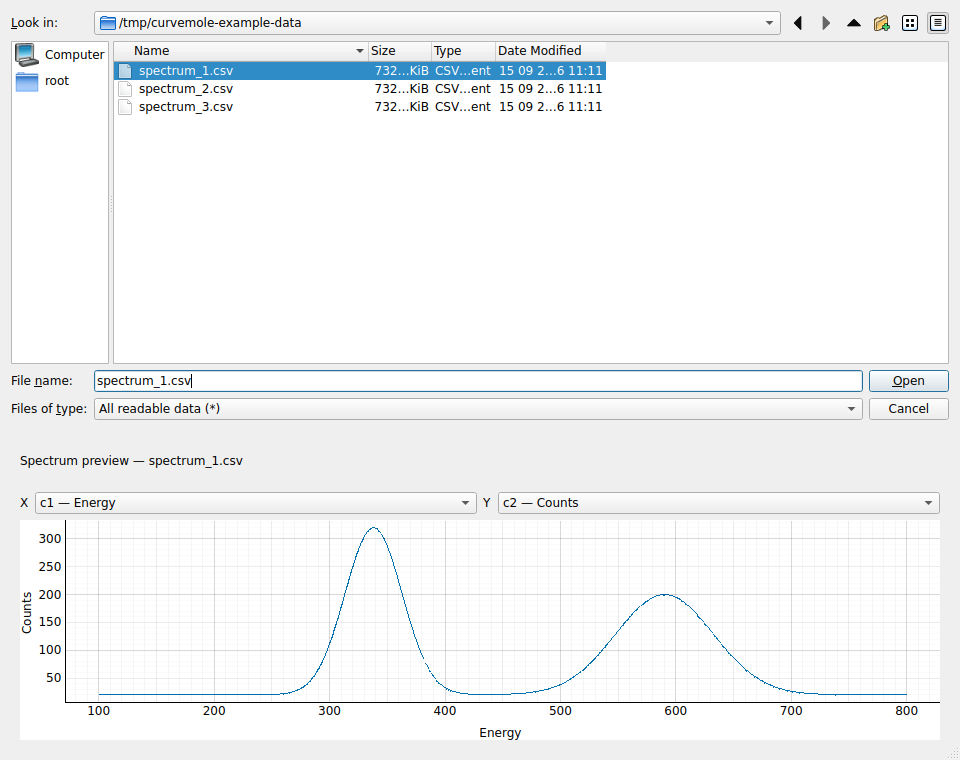
\includegraphics{screenshots/import-file-preview.png}
\caption{Preview while selecting files, before opening the import
mapping dialog.}
\end{figure}

\hypertarget{column-mapping}{%
\section{6.3 Column mapping}\label{column-mapping}}

\textbf{Destination} lets you create a new series or select an existing
series by name. A new series requires a unique non-empty name. Selecting
an existing series appends new spectra there while preserving its
identity, existing spectra, notes and palette. The destination applies
to every selected file in that import; later per-file mapping dialogs
keep it fixed. Cancelling a later mapping or failing to parse any file
leaves the destination unchanged. All files are parsed before any are
added.

Ordinary imports select one X and one active Y. All original columns
remain available in the imported curve. For files with more than two
columns, the \textbf{as separated files} checkbox appears directly below
the Y selection. Hover over it for an explanation. Enabling it imports
independent spectra in the same series, named after their Y headers (or
\texttt{Y\ -\ column\ N} without headers); it does not create files on
disk.

Choose the structure explicitly:

\begin{itemize}
\tightlist
\item
  \textbf{Shared X:} check multiple Y columns, all using the selected X.
  \textbf{Select all Y columns} selects every column except X; deselect
  any error or auxiliary columns before importing.
\item
  \textbf{Repeated groups:} choose the first column, number of Ys per X,
  and error type per Y, then click \textbf{Apply pattern}. One Y per X
  produces \texttt{XYXY...}; two produces \texttt{XYYXYY...}. With
  symmetric errors these become \texttt{XYE...} or \texttt{XYEYE...};
  asymmetric errors use \texttt{YE+E-} for each Y. Review or edit the
  resulting associations. Incomplete trailing spectra are excluded, and
  the unassigned column numbers are shown below the table.
\item
  \textbf{Custom:} add or remove spectrum rows and choose any X/Y
  associations, including nonadjacent columns and irregular groups.
  Switching from repeated groups to Custom retains the generated rows
  for editing.
\end{itemize}

Column names never infer the structure, axes, or error columns. Each
table row has its own error/weight type, error columns, and confidence
level. When an error type is enabled, its selector initially uses the
column immediately to the right of Y; asymmetric errors select the next
two columns as error + and error -, respectively. These defaults can be
changed. Missing columns or errors overlapping an assigned X/Y must be
resolved before importing. Error types initially remain \textbf{None}.
The same adjacent-column defaults apply to ordinary imports when errors
are enabled.

Optional columns are:

\begin{itemize}
\tightlist
\item
  \texttt{sigma\_x};
\item
  \texttt{sigma\_y};
\item
  Y error (confidence interval), or a pair of asymmetric Y error
  columns;
\item
  generic weight;
\item
  variance;
\item
  inverse variance.
\end{itemize}

Only one of \texttt{sigma\_y}, confidence-interval errors, generic
weight, variance, or inverse variance can be selected for a given
spectrum. Variance is converted to \texttt{sigma\_y} by square root.
\texttt{sigma\_x} is stored in the project but is not used by the
version 1.1.0 optimizer.

For confidence intervals, choose \textbf{Y error (confidence interval)}
and one symmetric half-width column, or check \textbf{Asymmetric error}
and select \textbf{Y error +} and \textbf{Y error -} separately. Both
columns contain positive magnitudes, not signed errors or interval
endpoints: the interval is
\texttt{{[}y\ -\ error\ -,\ y\ +\ error\ +{]}}. \textbf{Data error
confidence} declares its central coverage (default 95\%). This is
independent of the confidence selected for fitted parameter intervals.
Existing \texttt{sigma\_y} imports continue to mean one standard
deviation, regardless of this field. The import preview shows the
supplied errors at their original confidence.

The spectrum preview below the numeric table updates as you change X/Y
columns, uncertainty mappings, delimiter, decimal separator, header or
skipped rows. It plots the complete file, reusing the main graph's
peak-preserving downsampling and clipping rules. Parsed data are cached
while changing columns. Descending X is reversed for display;
nonmonotonic X is not clipped/downsampled. The view bounds always come
from full-resolution finite X/Y pairs. With no selected Y or an invalid
mapping, the preview clears and explains the problem. For batch import,
it previews the file named in the mapping dialog.

\hypertarget{batch-import}{%
\section{6.4 Batch import}\label{batch-import}}

When importing multiple files, \textbf{Apply this mapping to all files
in this batch} reuses the first file's parsing and column mapping.
Enable it only if all files truly share a layout. CurveMole does not
silently guess a new mapping for an incompatible file in the same batch.

Separated-spectrum mappings reuse column positions, so files with the
same layout can have different headers. Each spectrum keeps the Y name
from its own file. Ordinary batch mappings continue to use the selected
column names.

Files are imported in natural filename order: \texttt{scan\_2} precedes
\texttt{scan\_10}, regardless of the order returned by the file chooser.

\hypertarget{calibrated-winspec-spe-files}{%
\subsection{Calibrated WinSpec SPE
files}\label{calibrated-winspec-spe-files}}

CurveMole also reads binary WinSpec SPE 2.x files containing calibrated
one-dimensional acquisitions. The first column is wavelength in nm,
followed by one intensity column per frame. Select the frame through the
Y-column mapping. SPE 3.x, uncalibrated axes, images and multiple-ROI
acquisitions are unsupported; export those acquisitions to calibrated
x-y text before importing.

\hypertarget{automatic-folder-import}{%
\subsection{Automatic folder import}\label{automatic-folder-import}}

Choose \textbf{File \textgreater{} Automatic folder import\ldots{}} to
add arriving files to the current project. Select an existing folder, an
optional case-insensitive \textbf{Filename contains} filter, the
one-based X/Y columns and a \textbf{Wait for stable file} delay (2
seconds by default). Monitoring starts only when you press
\textbf{Start}.

\begin{itemize}
\tightlist
\item
  \textbf{Also import matching files already in the folder} includes
  existing files; otherwise the session starts with newly arriving
  files.
\item
  \textbf{Import changed files again as NEW spectra} retains the
  previous acquisition and adds a new one when file contents change.
\item
  \textbf{Show newest imported spectrum} controls whether successful
  imports take focus; it can be changed while monitoring runs.
\item
  \textbf{Automatic workflow} selects Import only or a loaded plugin's
  import processor. Configure the plugin first; processing runs on the
  new acquisition in the background before it is added to the live
  project.
\end{itemize}

Only files directly in the folder are scanned. Symlinks,
hidden/temporary files and projects are ignored, and automatic inputs
are limited to 256 MiB. Identical content at the same path is not
imported twice within a session. Each successful acquisition is one Undo
operation. Failed files appear in the log; correct them or the settings
and choose \textbf{Retry failed files}. Imports wait while fitting, a
desktop automation or a modal dialog is active. Closing the monitor
panel leaves it running; choose \textbf{Stop} or \textbf{File
\textgreater{} Stop automatic import} to stop. Changing projects ends
the session, and reopening CurveMole does not start monitoring
automatically.

\hypertarget{invalid-numeric-cells}{%
\section{6.5 Invalid numeric cells}\label{invalid-numeric-cells}}

Non-numeric cells are converted to missing numeric values. Rows are
retained in the stored arrays but excluded from fitting when x or y is
not finite. A row is also excluded if:

\begin{itemize}
\tightlist
\item
  \texttt{sigma\_y} is non-finite or not strictly positive;
\item
  a point weight is non-finite or negative;
\item
  it is masked;
\item
  it lies outside active fit ranges defined through the core API.
\end{itemize}

CurveMole does not reorder rows, average duplicate x values, or
interpolate missing values during import.

\hypertarget{uncertainties-and-weights}{%
\section{6.6 Uncertainties and
weights}\label{uncertainties-and-weights}}

If absolute \texttt{sigma\_y} values are supplied, point residuals are
scaled as:

\[
r_i^{(w)} = \frac{f(x_i)-y_i}{\sigma_{y,i}}.
\]

If inverse variances \(w_i=1/\sigma_i^2\) are supplied, CurveMole
multiplies residuals by \(\sqrt{w_i}\). A generic weight column directly
multiplies residuals by its value. This distinction is intentional and
is recorded in the curve metadata.

Zero generic weight is allowed and gives a point zero numerical
influence. A zero or negative \texttt{sigma\_y} is invalid and excludes
the row.

For a confidence level \(C\), interval half-widths are converted to
approximate Gaussian scales by dividing each side by
\(z=\Phi^{-1}((1+C)/2)\). At every evaluation, a prediction above the
measured value uses the upper scale; a prediction below uses the lower
scale. Equal half-widths reproduce symmetric Gaussian weighting. The
error arrays and confidence are saved and exported; plotted bars keep
the supplied half-widths, rather than these converted scales.

\textbf{Fit \textgreater{} Advanced algorithm options \textgreater{} Use
data errors / weights in the fit} is on by default. Turn it off to fit
without imported Y errors or point weights. Masks, fit ranges and
spectrum-level weights remain in effect. Rows invalid only because of
their error or point weight can then participate. The display of bars
and the noise model of Monte Carlo remain independent of this choice.

This is an approximation: two interval half-widths and a confidence
level do not specify the full measurement distribution. The scales
describe a Gaussian side on each side of the reported value; Monte Carlo
assigns equal probability to the two sides, reproducing the supplied
central interval. Covariance is a local Jacobian approximation, and
asymmetrical parameter intervals should be assessed using resampling or
a suitably calibrated profile. Correlation between measured points and X
uncertainty are not incorporated into this Y-residual fit.

Use \textbf{Error bars} above the main graph to show or hide the bars.
Autoscaling includes their endpoints, and bars follow logarithmic,
waterfall and background views. Scalar and curve scaling propagate
widths and exchange upper/lower sides for negative factors. Custom and
column formulas use local derivative propagation; for strongly nonlinear
transformations this is only a local approximation.

\hypertarget{curves-masks-and-transformations}{%
\chapter{7. Curves, masks, and
transformations}\label{curves-masks-and-transformations}}

\hypertarget{immutable-originals}{%
\section{7.1 Immutable originals}\label{immutable-originals}}

CurveMole preserves imported x, y, uncertainty, and weight arrays.
Displayed working arrays are reconstructed by applying a transformation
history to the originals. This design makes data preparation reversible
and auditable.

\hypertarget{masking-points-and-intervals}{%
\section{7.2 Masking points and
intervals}\label{masking-points-and-intervals}}

Masked points remain stored but are excluded from fitting. They are
drawn as faded markers, and masked intervals are shaded.

Enable the graphical \textbf{Mask} button: right-drag masks an interval
and left-drag unmasks it. A right/left click performs the equivalent
operation on a point. The button becomes grey while active. Turn it off
to navigate without changing exclusions. Changing display mode also
exits masking.

\hypertarget{mask-targets}{%
\section{7.3 Mask targets}\label{mask-targets}}

\begin{longtable}[]{@{}ll@{}}
\toprule
Target & Effect\tabularnewline
\midrule
\endhead
Active & Changes only the active curve\tabularnewline
All visible & Changes every currently visible curve\tabularnewline
\bottomrule
\end{longtable}

Single view always uses the active spectrum. Overlay and Waterfall
prompt for Active or All visible when entering Mask mode; cancelling
leaves masking off.

For interval masks, the same numeric x interval is applied to every
target. For a single-point mask transferred from the active curve,
CurveMole locates the nearest x value on other targets and applies it
only if it lies within the configured tolerance.

Set this tolerance through \textbf{Data \textgreater{} Mask transfer
tolerance}. A value of zero requires an exact matching x value on
transferred point masks.

\hypertarget{undo-and-mask-history}{%
\section{7.4 Undo and mask history}\label{undo-and-mask-history}}

A graphical mask action is placed on the application Undo stack. Press
\textbf{Ctrl+Z} to undo it or \textbf{Ctrl+Y} to redo it. The project
also stores mask arrays and numeric mask intervals.

Fits, including Quick Fit and sequential fitting, also support
Undo/Redo. Undo restores the pre-fit models, parameter values, fit
results, and sequential pause state; Redo restores the completed fit
without running the solver again. Cancelled or failed worker operations
restore the previous state. The Undo stack retains the latest 20
operations (fits and other edits combined); input data arrays are not
duplicated for fit history. Undo/Redo are disabled while a worker is
running.

Quick Fit is available before opening Fit\ldots: its first run uses the
default independent-fit settings on the selected curves, falling back to
the active curve. Later runs retain the configured solver, loss and
algorithm settings but always use \textbf{Single/Independent}, even
after a sequential or global fit. Open Fit\ldots{} to use another
fitting mode.

\hypertarget{data-calculator}{%
\section{7.5 Data Calculator}\label{data-calculator}}

Open \textbf{Tools \textgreater{} Data Calculator}. The following scalar
operations are available:

\begin{itemize}
\tightlist
\item
  add to or subtract from y;
\item
  multiply or divide y;
\item
  shift x;
\item
  scale x;
\item
  normalize y by maximum absolute value;
\item
  normalize y by signed integrated area.
\end{itemize}

Every calculator operation (including restoring data) offers
\textbf{Active curve} or \textbf{Choose multiple spectra\ldots{}}. The
picker initially shows the active series; \textbf{All series} shows
every spectrum grouped under colored series headings. Use checkboxes or
Select all shown. Hidden spectra are excluded. Cancel changes nothing. A
batch is checked in full before any spectrum is modified; one Undo
restores the whole batch. Normalization also scales \texttt{sigma\_y}
consistently. Dividing by zero and normalizing a zero or invalid signal
are rejected.

\hypertarget{advanced-column-formulas}{%
\subsection{Advanced column formulas}\label{advanced-column-formulas}}

The note below Formula reminds you to use Python syntax for mathematical
operators.

The green \textbf{Advanced - column formula} entry is first in the
operation list, followed by the green \textbf{Custom formula} for a
single plotted axis. New imports retain every source column as numeric
data in the project, including columns not plotted. Original column
order and row alignment are preserved. \texttt{c1}, \texttt{c2},
\texttt{c3}, etc. refer to one-based source columns; \texttt{x} and
\texttt{y} refer to the current plotted axes. \textbf{Insert into
formula} lists the available codes with original column names; choose an
entry, then press \textbf{Insert} to add its code at the cursor.
\textbf{Write result to} chooses X, Y or any retained column for the
result. The hint below it explains that Apply writes the formula result
into this column. Merely selecting an input column does not edit the
formula or change its destination. A live summary such as
\texttt{Y\ -\ Counts\ \textless{}-\ c2\ /\ c3**2} makes the direction
explicit. \textbf{Spectra to modify} separately chooses which spectra
receive the operation.

\begin{figure}
\centering
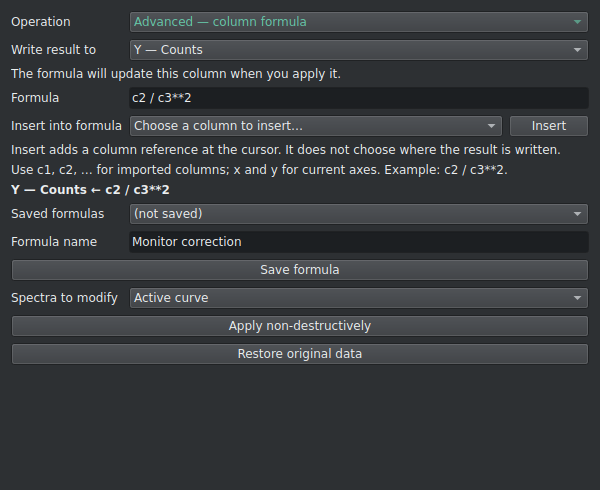
\includegraphics{screenshots/advanced-calculator-dark.png}
\caption{Advanced calculator with column insertion and destination
controls in dark mode.}
\end{figure}

For a file with Energy, Counts and Monitor columns, plotting c1 against
c2:

\begin{enumerate}
\def\labelenumi{\arabic{enumi}.}
\tightlist
\item
  choose \textbf{Advanced - column formula};
\item
  choose \textbf{Y - Counts} as the destination;
\item
  insert \texttt{c2} and \texttt{c3} from the dropdown to enter
  \texttt{c2\ /\ c3**2};
\item
  choose Active curve or multiple spectra, then Apply non-destructively.
\end{enumerate}

You can also enter \texttt{y\ /\ c3\^{}2} (\texttt{\^{}} and \texttt{**}
both mean exponentiation in Advanced), \texttt{c2\ -\ c4}, or
\texttt{sqrt(c5)}. A header may be referenced as
\texttt{\$\{Monitor\ counts\}}; codes remain unambiguous for unusual
names. Only restricted mathematical expressions are accepted, never
Python execution. Scalar results are broadcast to every row; missing
columns and non-finite output (including division by zero) reject the
batch. Masks do not change row alignment: formulas operate on all rows.

Writing to a plotted source column updates that axis. Writing to an
unplotted column leaves the graph unchanged and makes the new values
available to later formulas. Normal calculator operations on X/Y are
also reflected in their mapped columns. Calculations are local to each
spectrum, even when spectra originated in the same file. In a
multi-spectrum batch \texttt{cN} always means position N in each file;
check that the files have compatible layouts. Uncertainty propagation is
not inferred for custom formulas; changing an auxiliary uncertainty
column does not remap the uncertainty arrays originally selected for
fitting.

Name and \textbf{Save formula} to retain the expression and destination
in the project, then recall it through Saved formulas. Retained columns,
formulas and their Undo/Redo history survive \texttt{.fitproj} saving
without the original source file. Projects created before this feature
contain only their previously stored axes: re-import the source to
recover additional columns.

\hypertarget{curve-to-curve-calculations}{%
\section{7.6 Curve-to-curve
calculations}\label{curve-to-curve-calculations}}

The calculator can add, subtract, multiply, or divide by another curve.
The operand is aligned to the target x grid by:

\begin{itemize}
\tightlist
\item
  linear interpolation;
\item
  nearest-neighbor interpolation;
\item
  cubic spline interpolation.
\end{itemize}

Extrapolation is disabled by default. Outside the operand range, aligned
values become missing and will therefore be excluded from later fitting.
Enabling extrapolation is an explicit advanced choice. Cubic
interpolation requires at least four unique finite operand x values.

The aligned operand array is stored with the transformation so that
reopening the project does not depend on a later change to the source
curve.

\hypertarget{restoring-original-data}{%
\section{7.7 Restoring original data}\label{restoring-original-data}}

\textbf{Restore original data} removes all currently applied
transformations from the selected target while retaining them on the
redo stack. The imported arrays are not re-read from disk. The whole
action is also integrated with application Undo.

\hypertarget{worksheet}{%
\section{7.8 Worksheet}\label{worksheet}}

The Worksheet is a read-only inspection view. It shows up to 100,000
rows for the active curve with columns for x, y, \texttt{sigma\_y},
weight, and mask state. It is not a spreadsheet editor and does not
modify source arrays.

\hypertarget{editing-individual-data-points}{%
\section{7.9 Editing individual data
points}\label{editing-individual-data-points}}

Choose \textbf{Data \textgreater{} Edit data points\ldots{}} to edit
measured points directly in the graph. The editing controls appear above
the plot. Only the active, displayed dataset is edited; the original
source coordinates remain immutable.

\begin{enumerate}
\def\labelenumi{\arabic{enumi}.}
\tightlist
\item
  Click a point to select it. Its current X/Y coordinates appear in the
  editing bar.
\item
  Choose \textbf{X}, \textbf{Y}, or \textbf{XY} to constrain the data
  coordinates that may change.
\item
  Drag the point and release to commit one undoable move. During
  dragging, the graph previews the new position without changing the
  saved dataset.
\item
  Use \textbf{Delete selected point}, \textbf{Delete}, or
  \textbf{Backspace} to remove it. At least two points must remain.
  Deletion removes the row from current data, fitting, worksheets and
  numeric exports, keeping associated errors, weights, masks and
  auxiliary columns aligned.
\item
  Choose \textbf{Done} or press \textbf{Esc} to leave editing. Esc also
  discards an unfinished drag; previously completed moves and deletions
  remain applied.
\end{enumerate}

Right-drag pans and the wheel zooms while editing. Point selection uses
the actual samples, including in dense plots. Logarithmic axes,
Waterfall offsets and visual background subtraction are accounted for;
the editing bar shows the underlying data coordinates. X/Y constraints
refer to those data coordinates.

Moves and deletions use the global \textbf{Undo/Redo} commands. They are
stored in the project as reversible transformations and can also be
removed with \textbf{Restore original data} in the Data Calculator. A
changed fitted dataset is marked as modified, so refit it to update
results and uncertainties. Entering function placement, changing the
active dataset or starting a calculation ends point editing. Read-only
projects cannot be edited.

\hypertarget{building-models}{%
\chapter{8. Building models}\label{building-models}}

All entries in the function library are fitting functions. Constant,
linear, polynomial, cubic-spline, peak-shaped, and custom formulas are
not separated into a special background-function class. Background is
instead a property of a model component. Select a component in
\textbf{Model and parameters} and enable \textbf{Mark as background}
when that component represents the experimental baseline or background.

\textbf{Data \textgreater{} Subtract background\ldots{}} uses these
component-level marks. If no component is marked, CurveMole first asks
which model functions should be designated as background. If background
components already exist, it asks which of the marked components should
be subtracted. The subtraction uses the current resolved/fitted
parameter values, is reversible with Undo, applies over the complete
data array, and disables the subtracted components afterwards to prevent
double-counting.

The \textbf{Subtracted} / \textbf{Not subtracted} labels follow the
subtraction history of each spectrum. Copying a fit preserves the
destination's existing subtraction; it does not subtract the source
background from the destination's data. The saved subtraction retains
the parameter values used at that time. Editing or copying later
parameter values does not recalculate it. A duplicated function starts
with its own history and is not marked as subtracted merely because its
source was. On opening older projects, CurveMole can reconnect a
recorded subtraction to a uniquely identified builtin background whose
internal ID changed. This restores the label and function-state
restoration without changing the measured data, the stored subtraction
array or the current fitted parameter values. If the old history is
ambiguous, the label reads \textbf{Subtraction recorded - function
uncertain}; \textbf{Revert background} still uses the actual recorded
array. Confirming Revert removes the subtraction, so \textbf{Not
subtracted} is then the expected status.

The same dialog can apply the operation to every eligible spectrum,
using the enabled functions already marked as background in each model.
\textbf{Data \textgreater{} Revert background\ldots{}} lists only
spectra changed by this dedicated subtraction command and restores the
selected ones, including the relevant function states. \textbf{View
options \textgreater{} Background \textgreater{} Remove fitted
background in this view} instead removes the enabled marked background
only from the plot; it never changes curve arrays, fit inputs, or
exported values.

The \textbf{View options (display only)} toolbar button opens a menu
with \textbf{Current spectrum} and \textbf{All spectra} scopes. The menu
explicitly states that data are not modified and operations are not
undone. Scope selects the targets for the next display change; it does
not change views by itself. All spectra includes hidden spectra, which
use the chosen view when displayed later. Per-spectrum choices follow
spectrum navigation.

\begin{itemize}
\tightlist
\item
  \textbf{Preview stored data - all operations included} closes display
  filters for the scope.
\item
  \textbf{Preview original data - without processing or masks} shows the
  imported X/Y values, including visually deleted points, without
  displaying the effects of masks or processing. The stored data, masks
  and processing history remain unchanged.
\item
  \textbf{Show data before background subtraction} omits recorded
  background subtractions and replays the remaining operations in order.
  It also works after the background functions have been disabled by a
  real subtraction.
\item
  \textbf{Operations included in preview} allows individual display
  exclusions on the current spectrum. In All spectra scope, entries are
  grouped by operation type with a count such as \textbf{Y
  multiplication - 3/5 spectra}. Unchecking a type excludes every
  occurrence on spectra that contain it; spectra without that type are
  unaffected. Different numeric parameters do not prevent grouping.
  Mixed inclusion states are labelled. Unchecking an operation only
  hides its effect in the preview; it does not undo it.
\end{itemize}

All exclusions replay the retained recorded operations in their original
order, using their recorded parameters and array operands. A later
operation can depend on rows removed by an earlier one. An incompatible
combination is rejected for the entire scope, with an explanation; the
last valid view remains visible. Recorded Y replacements remain absolute
replacements when replayed.

Models, residuals and plugin annotations are hidden for
reconstructed/original data because their fits refer to the stored
processed data. Error bars and framing use the displayed arrays. The
banner always states \textbf{Display only} and \textbf{Data unchanged;
no operations undone}. \textbf{Close all previews} returns every
spectrum to its stored display; \textbf{Close preview for this scope}
affects only the chosen scope. Starting an edit, mask operation,
graphical placement or fit closes reconstructed previews and uses the
stored data and processing. Background-only visual subtraction remains
compatible with the normal fit overlay. These preview choices are
temporary and do not modify processing history, Undo/Redo, exports or
the saved project's scientific data.

During graphical cubic-spline placement, nodes may be placed anywhere in
plot coordinates, including outside the x/y extent of the measured data.
Adding nodes does not auto-range the graph. Left-drag continues to pan
and the mouse wheel continues to zoom while placement is active.

\hypertarget{component-composition}{%
\section{8.1 Component composition}\label{component-composition}}

New models use \textbf{global function roles}, independent of insertion
and display order.

\begin{longtable}[]{@{}ll@{}}
\toprule
Operator & Global role\tabularnewline
\midrule
\endhead
\texttt{add} & Include the function in the starting sum\tabularnewline
\texttt{subtract} & Subtract the function from the starting
sum\tabularnewline
\texttt{multiply} & Multiply the whole intermediate model by the
function\tabularnewline
\texttt{divide} & Divide the whole intermediate model by the
function\tabularnewline
\texttt{convolve} & Convolve the whole intermediate model with the
function\tabularnewline
\bottomrule
\end{longtable}

For example, two Add peaks G1 and G2 plus a Multiply function M produce
\texttt{(G1\ +\ G2)\ *\ M}, regardless of which function was added
first. Additive peaks and backgrounds normally use Add. Background
marking requires Add or Subtract; unmark a background before changing it
to a factor or kernel.

\textbf{Calculation order} lists individual Multiply, Divide and
Convolve functions. Move them up/down or drag them to choose application
order, from top to bottom. Its expression preview distinguishes
\texttt{convolve((G1\ +\ G2)\ *\ M,\ R)} from
\texttt{convolve(G1\ +\ G2,\ R)\ *\ M}; those calculations can give
different results. Only OK applies the choice; Cancel discards it.
Changes support Undo/Redo and persist in projects, model files and
copied structures. Without an explicit choice the default is
multiplication, then division, then convolution, independent of
insertion order.

With no Add/Subtract terms, multiplication and division start from 1; a
convolution without a preceding signal starts with its first kernel. One
Multiply function is therefore itself, one Divide function is its
reciprocal, and one Convolve function is itself. An empty or fully
disabled model is zero. Consecutive convolutions use full FFT
convolution with uniform x-spacing scaling and crop once back to the
input length, so inserting the same kernels in another order does not
change edge handling. FFT convolution requires a finite, uniformly
spaced, strictly monotonic X axis; resample irregular data onto a
regular grid first. Ascending and descending grids are supported. Masks
and fit ranges select residuals after evaluation on the full current
data grid: excluding points does not change the convolved model itself.
Marked additive backgrounds receive the same global factors and
convolutions as the full model when their contribution is evaluated.

The same global roles apply to every project, model file and workflow,
including files saved by earlier versions. There is no separate
ordered-composition mode or first-function restriction. A model
previously calculated in insertion order can produce a different result
with global roles: review its expression in Calculation order and refit
after opening it.

Division by a component that reaches zero and other non-finite model
evaluations are rejected by the fitter.

\hypertarget{built-in-peak-parameterization}{%
\section{8.2 Built-in peak
parameterization}\label{built-in-peak-parameterization}}

Every built-in peak uses signed integrated \texttt{area}, not peak
height, as its intensity parameter. Negative areas produce negative
peaks. This common parameterization makes areas comparable between
different line shapes.

\hypertarget{gaussian}{%
\subsection{Gaussian}\label{gaussian}}

Parameters: \texttt{area}, \texttt{center}, \texttt{sigma}.

\[
G(x)=\frac{A}{\sigma\sqrt{2\pi}}
\exp\left[-\frac{1}{2}\left(\frac{x-x_0}{\sigma}\right)^2\right].
\]

The derived FWHM is \(2.354820045\,\sigma\). \texttt{sigma} is
intrinsically positive.

\hypertarget{lorentzian}{%
\subsection{Lorentzian}\label{lorentzian}}

Parameters: \texttt{area}, \texttt{center}, \texttt{gamma}.

\[
L(x)=\frac{A\gamma}{\pi[(x-x_0)^2+\gamma^2]}.
\]

\texttt{gamma} is the half width at half maximum, so FWHM is
\(2\gamma\). \texttt{gamma} is intrinsically positive.

\hypertarget{voigt}{%
\subsection{Voigt}\label{voigt}}

Parameters: \texttt{area}, \texttt{center}, \texttt{sigma},
\texttt{gamma}.

The Voigt component is the area-normalized convolution of a Gaussian
with standard deviation \texttt{sigma} and a Lorentzian with HWHM
\texttt{gamma}. CurveMole evaluates it with the SciPy Voigt profile.
Both width parameters are intrinsically positive.

The displayed FWHM is the approximation:

\[
\mathrm{FWHM}\approx 0.5346(2\gamma)+
\sqrt{0.2166(2\gamma)^2+(2.354820045\,\sigma)^2}.
\]

\hypertarget{pseudo-voigt}{%
\subsection{Pseudo-Voigt}\label{pseudo-voigt}}

Parameters: \texttt{area}, \texttt{center}, \texttt{fwhm}, \texttt{eta}.

The profile is an area-normalized linear mixture with a common FWHM:

\[
pV(x) = A[(1-\eta)G_{\mathrm{unit}}(x)+\eta L_{\mathrm{unit}}(x)].
\]

\texttt{fwhm} is intrinsically positive and \texttt{eta} is
intrinsically bounded to \([0,1]\). \texttt{eta=0} is Gaussian and
\texttt{eta=1} is Lorentzian.

\hypertarget{built-in-functions-commonly-used-as-backgrounds}{%
\section{8.3 Built-in functions commonly used as
backgrounds}\label{built-in-functions-commonly-used-as-backgrounds}}

The library names are \textbf{Constant}, \textbf{Linear},
\textbf{Polynomial} and \textbf{Cubic spline}. They become background
components only when \textbf{Add as background} in the Add dialog or
\textbf{Mark as background} in the model panel is enabled.

\hypertarget{constant}{%
\subsection{Constant}\label{constant}}

Parameter: \texttt{offset}.

\[
B(x)=c.
\]

\hypertarget{linear}{%
\subsection{Linear}\label{linear}}

Parameters: \texttt{intercept}, \texttt{slope}.

\[
B(x)=c_0+c_1x.
\]

\hypertarget{polynomial}{%
\subsection{Polynomial}\label{polynomial}}

Choose an order from 0 to 50 when adding the component. Parameters are
\texttt{c0}, \texttt{c1}, and so on through the chosen order:

\[
B(x)=\sum_{k=0}^{n}c_kx^k.
\]

High polynomial orders are numerically sensitive when x values are large
or poorly scaled. Prefer a low order or rescale x with the Data
Calculator when scientifically appropriate.

\hypertarget{cubic-spline}{%
\subsection{Cubic spline}\label{cubic-spline}}

Spline x nodes are metadata, rather than optimizer parameters. Their y
values (\texttt{y0}, \texttt{y1}, and so on) are normal parameters that
may be fitted, fixed, bounded, or linked. Two nodes produce linear
interpolation. Three or more nodes produce a natural cubic spline, with
extrapolation outside the node range.

New graphically placed spline y nodes are fixed by default so an
intentionally drawn baseline does not move when fitting begins. Uncheck
\textbf{Fixed} for individual nodes, or use \textbf{Lock all} /
\textbf{Unlock all} below the parameter table for every parameter in the
selected function. The spline remains continuous through masked
intervals even though masked measurements do not contribute to the
objective function.

\hypertarget{functions-selection-insertion-and-details}{%
\section{8.4 Functions: selection, insertion and
details}\label{functions-selection-insertion-and-details}}

Choose a registered function from the selector inside the
\textbf{Functions} toolbar group and press its \textbf{Add} button. The
list includes built-in peaks and backgrounds, generic functions,
project-contained formulas, reusable formulas, and trusted plugin
functions. The last choice is remembered. Below the selector, check
\textbf{Background} to mark the added function as background and
\textbf{Initialize with points} to initialize it from graph points. Both
options default to off.

\begin{itemize}
\tightlist
\item
  a peak with \textbf{Initialize with points} checked allows repeated
  centre/FWHM click-drags until \textbf{Finish}, right-click or
  Return/Enter ends placement; its parameters remain free for fitting;
\item
  a peak with that option cleared is added immediately, one per
  \textbf{Add} click. CurveMole estimates centre, height and width from
  the most prominent positive or negative peak in the finite, unmasked
  data minus the current model. Repeated clicks estimate the remaining
  residual peaks. Short or flat data use a finite fallback estimate; all
  estimates can be edited before fitting;
\item
  a cubic spline with \textbf{Initialize with points} enabled opens
  point-by-point node placement;
\item
  Linear and other functions use manual-point placement only when
  explicitly enabled using \textbf{Initialize with points};
\item
  non-peak functions with point initialization off are added with their
  initial parameters; a spline in this mode uses an initial node grid
  with free y parameters.
\end{itemize}

The arrow beside \textbf{Add function} chooses how the new function
combines with the existing model: \textbf{Add (+)}, \textbf{Subtract
(-)}, \textbf{Multiply (x)}, \textbf{Divide (/)}, or **Convolve (*)**.
The orange symbol on the insertion icon shows the current choice;
clicking the main part of the button inserts with that composition. The
same choice is available in Function details and the advanced Add dialog
and is remembered. All roles are available in every model, including for
the first function. Background marking is available for Add and Subtract
only. For automatic or graphical peak initialization, Add uses data
minus the existing model, Subtract uses model minus data, Multiply uses
data/model, and Divide uses model/data. Non-finite ratios are excluded.
Automatic convolution inserts a kernel centred on the sampled domain;
built-in area-normalized peaks start with unit area. All initial
estimates remain editable.

The Functions group uses the shared function registry and peak parameter
roles, including roles supplied by user formulas and plugins. Selecting
a function in the normal Add dialog also makes it the next toolbar
choice. The Functions group remembers its own manual-point and
background options separately for each function. It does not inherit
options from the normal Add dialog or its older shared preferences.
Changing the point option during peak placement cancels the pending peak
without adding anything; already completed peaks remain. Switching to an
automatic peak in the selector also waits for the next \textbf{Add}
click.

The \textbf{Function details} button (a function card with a curve and
formula), inside the Functions group, replaces the old toolbar Add
component button. It follows the selected function and opens a reference
with its formula, description, default parameters, bounds, units,
derived quantities and initialization instructions. Its
\textbf{Function} selector also lets you choose any other registered
function, including formulas and plugin functions. This selector and the
toolbar selector stay synchronized; the reference updates immediately.
Browsing does not add a component and cancels unfinished graphical
placement without removing components already added. \textbf{Copy
formula} copies the displayed expression; \textbf{Add function} opens
the advanced Add component dialog with that function selected. The Model
menu and Ctrl++ still open that dialog directly. Plugin formulas are
displayed when supplied by the provider.

In the Functions group's point placement, right-click and Return/Enter
commit the same points as \textbf{Finish}, provided the minimum has been
reached; otherwise placement stays active. \textbf{Undo point} removes
the most recent point. In the regular Add dialog's point placement,
right-click continues to remove the nearest point.

\hypertarget{adding-a-peak-with-the-pointer}{%
\section{8.5 Adding a peak with the
pointer}\label{adding-a-peak-with-the-pointer}}

In the toolbar Functions group, choose a peak, enable \textbf{Initialize
with points}, and press \textbf{Add function}:

\begin{enumerate}
\def\labelenumi{\arabic{enumi}.}
\tightlist
\item
  click the intended center;
\item
  drag horizontally to either half-height edge;
\item
  release to set the initial full width.
\end{enumerate}

A green region previews the width. If no horizontal width is selected,
CurveMole uses a default based on 5 percent of the x span, local point
spacing, and floating point precision.

For built-in peaks, CurveMole converts the graphical height and FWHM
into the native area and width parameters. New custom peaks should
declare explicit semantic roles for their position, intensity, and width
parameters in Function Builder. Older custom functions without role
metadata retain compatibility through conventional names such as
\texttt{center}, \texttt{x0}, \texttt{fwhm}, \texttt{sigma},
\texttt{gamma}, \texttt{area}, \texttt{amplitude}, or \texttt{height}.

\hypertarget{construction-options-and-initial-parameters}{%
\subsection{Construction options and initial
parameters}\label{construction-options-and-initial-parameters}}

\textbf{Add function} asks for construction options when the selected
function declares them. For \textbf{Polynomial}, choose its degree
(0-50) before adding it when \textbf{Initialize with points} is
disabled. In point mode, options declared as derivable from points are
not requested beforehand: N distinct polynomial points define degree
N-1. The current degree appears in the placement instructions. Removing
a point reduces the degree, and moving a point recalculates the
coefficients. Cancel leaves the model unchanged. The last confirmed
construction options are remembered per function and shared with the
advanced Add dialog. Background and point-initialization choices still
apply. Functions without construction options retain immediate
insertion.

In the advanced \textbf{Add component} dialog, the parameter table
provides \textbf{Initial value}, \textbf{Minimum}, \textbf{Maximum}, and
\textbf{Fixed} for every parameter. Construction options update the
table; changing polynomial degree preserves edits to coefficients that
remain present. Limits apply to the subsequent fit as well as
initialization. Use \texttt{-inf} and \texttt{inf} for unbounded limits
within the function's allowed domain. Invalid values are highlighted and
prevent insertion until corrected.

\textbf{Restore defaults} restores the selected configuration's
parameter values, bounds, and fixed states. \textbf{Estimate from data}
estimates values using usable, unmasked points of the active spectrum,
respecting bounds and leaving fixed parameters unchanged. This is a
standalone component estimate against the spectrum, not a fit of the
complete composed model. Inspect and edit the estimate before adding.
With manual-point initialization disabled, \textbf{OK} inserts exactly
the displayed configuration, including for peaks and splines; no later
automatic or graphical estimate replaces it. Enabling manual-point
initialization disables the table and its estimation controls because
the selected graph points determine those values.

Developers and plugin authors can declare
\texttt{FunctionDefinition.configuration\_specs} using
\texttt{FunctionOptionSpec} (integer, number, boolean, text, or choice).
An option's \texttt{from\_points(x,\ y)} callback declares how graph
points determine it. Only options without that callback are requested in
point mode. \texttt{FunctionDefinition} can also declare
\texttt{point\_initializer(x,\ y,\ metadata)} and
\texttt{minimum\_points}; the same rules are used for previews and
insertion, including custom and plugin functions. The same controls,
validation and component metadata are used by quick and advanced
insertion. Polynomial initialization solves on a scaled domain, then
converts to the existing \texttt{c0\ +\ c1*x\ +\ ...} coefficient
convention. Numerically unreliable point sets block Finish with an
explanation; previews of inferred functions stay within the selected
point interval to avoid misleading extrapolation.

\hypertarget{initializing-any-function-from-manually-selected-points}{%
\section{8.6 Initializing any function from manually selected
points}\label{initializing-any-function-from-manually-selected-points}}

In Add component, enable \textbf{Initialize from manually selected
points on the graph}. This is selected by default for Linear and Cubic
spline and can be used for other built-in, custom or plugin functions.
For a custom formula, Function Builder can set \textbf{Use manual-point
initialization by default}.

Click explicit points representing the function you want to create. A
live green function preview updates as points are added or removed; it
is an initial estimate, not a fit to the measured spectrum. Linear
requires at least two points. Other non-spline functions normally
require at least two points and at least as many points as parameters.
Point-derived configurations can declare their own minimum; Polynomial
starts with two distinct x positions and adapts its degree as points are
added or removed. Cubic spline requires at least two distinct x
positions.

The placement bar offers \textbf{Add points}, \textbf{Delete points} and
\textbf{Move points}. Delete points removes the point you click;
clicking empty space does nothing. Move points lets you click and drag a
point to a new x/y position, with a live function preview. Drag empty
space to pan and use the mouse wheel to zoom. \textbf{Undo point}
reverses the last addition, deletion or completed move. These edits
affect the function's initialization points, leaving the experimental
data unchanged.

Use \textbf{Finish} (or double-click in Add points mode) to commit after
the minimum number of points. Deleting below that minimum disables
Finish until enough points are restored or added. In Quick Add,
right-click or Enter also finishes; in the advanced Add component flow,
right-click removes the nearest point. \textbf{Esc} cancels the whole
insertion. The resulting parameters are fixed by default. Use
\textbf{Unlock all} or individual \textbf{Fixed} checkboxes before
optimizing them. Points and the corresponding controls are stored with
the component and project.

\hypertarget{reopening-a-functions-control-points}{%
\subsection{Reopening a function's control
points}\label{reopening-a-functions-control-points}}

Right-click a function in \textbf{Model and parameters} and choose
\textbf{Edit function points} (the same command is in \textbf{Model}).
Saved control points reopen in the placement bar, initially in
\textbf{Move points} mode. Switch to \textbf{Add points} or
\textbf{Delete points} as needed; \textbf{Undo point}, pan, zoom and the
live preview remain available. Polynomial degree follows the current
point count. This works for every function with saved manual points,
including custom and plugin functions. Older graphical peaks without
stored points can reconstruct controls from their current shape; normal
peak centre/width handles remain available outside this editor. Peak
controls follow the current shape after fitting or dragging, and
finishing without moving points leaves the function unchanged. Peak
edits use the same estimate in the live preview and on Finish.

For a function marked \textbf{Background}, the active spectrum
temporarily displays without background subtraction, including a display
reconstruction of recorded subtractions. Other spectra retain their
display options. Non-background functions keep the current background
display. Opening the editor or cancelling changes only the view. On
\textbf{Finish}, a background that was already subtracted is
recalculated with its new function, replacing its existing subtraction
rather than subtracting it twice. Grouped backgrounds and later
processing are replayed together. The function change and updated
subtraction form one \textbf{Undo}/\textbf{Redo} operation; original
imported arrays remain unchanged. A background that has not yet been
subtracted is only updated as a model function.

\textbf{Finish} updates the selected function in place, preserving its
identity, name, composition and background role, as one
\textbf{Undo}/\textbf{Redo} operation. Existing bounds, fixed states and
links for retained parameter names are preserved; deleting a parameter
referenced by another function is rejected. \textbf{Cancel} or
\textbf{Esc} discards the draft; changing spectrum/function or starting
another edit also cancels it. The previous display options and viewport
return when the editor closes. Control points are saved with the project
and remain editable after reopening it.

\hypertarget{drawing-a-cubic-spline-background}{%
\subsection{Drawing a cubic-spline
background}\label{drawing-a-cubic-spline-background}}

After choosing \textbf{Cubic spline}, enable \textbf{Add as background}
and keep manual-point initialization enabled:

\begin{enumerate}
\def\labelenumi{\arabic{enumi}.}
\tightlist
\item
  left-click background nodes on the plot;
\item
  inspect the live green preview, which updates after each click;
\item
  use \textbf{Undo point} if necessary;
\item
  finish with \textbf{Finish} or double-click after at least two nodes;
  right-click removes the nearest node;
\item
  press \textbf{Esc} to cancel the entire placement.
\end{enumerate}

Nodes are sorted by x. Clicking again at effectively the same x updates
that node instead of creating a duplicate. Exact duplicate x positions
are not permitted.

\hypertarget{graphical-editing-after-placement}{%
\section{8.7 Graphical editing after
placement}\label{graphical-editing-after-placement}}

Select a peak component to display its handles. Drag the central target
to change center and area-derived height. Drag a side line to change
FWHM. For a Voigt peak, changing FWHM graphically scales \texttt{sigma}
and \texttt{gamma} by the same ratio, preserving their current relative
contribution.

For a function created from manual points, selecting it displays its
original control points. Unlock the relevant parameters before dragging
a point in x and y. For a spline, unlock that node's y parameter:
dragging also updates its stored x position and keeps nodes sorted. For
other functions, at least one parameter must be free; CurveMole refines
those free values against the moved control points while retaining fixed
and linked values. Each completed drag is undoable. Exact numeric
parameter edits are available in the table.

For normal peak centre/width handles, fixed values cannot normally be
changed by a drag. Hold \textbf{Ctrl} while dragging to change the
stored value while leaving the parameter fixed. Manual-point handles
instead require unlocking the relevant parameters. Linked values cannot
be dragged independently because an expression controls them.

\hypertarget{automatic-peak-suggestions}{%
\section{8.8 Automatic peak
suggestions}\label{automatic-peak-suggestions}}

Choose \textbf{Model \textgreater{} Find positive peaks\ldots{}}.
Despite the menu label, the first dialog can search positive, negative,
or both signs. The next dialog selects any registered function
classified as a peak, initially preferring the peak selected in the
Functions group. CurveMole then:

\begin{itemize}
\tightlist
\item
  subtracts the median as an initial baseline;
\item
  estimates noise through a robust median absolute deviation;
\item
  uses a default prominence of the larger of three noise estimates or 1
  percent of the y range;
\item
  estimates width at half prominence;
\item
  sorts suggestions by prominence.
\end{itemize}

Choose how many suggestions to add. Every suggestion is initialized
using the selected peak function's explicit parameter roles or, for
legacy functions, recognized parameter names. Suggestions are initial
estimates, not a scientific decision about the number, identity, or line
shape of peaks.

\hypertarget{duplicating-disabling-deleting-and-reordering}{%
\section{8.9 Duplicating, disabling, deleting, and
reordering}\label{duplicating-disabling-deleting-and-reordering}}

Duplicate a component to create an adjacent copy with a new internal
identifier. Disable a component to compare models without losing its
settings. Deletion and reordering are undoable. In global models the
function list order is independent of the mathematical order; use
Calculation order to change precedence explicitly.

The \textbf{Reorder} button sorts the function list in ascending
parameter order (peak \texttt{center}, or X position, by default),
including peaks of different types. It also renumbers automatically
named functions within each type to match that order. IDs, links and
custom names are preserved; custom-named functions are sorted too.
Functions without a finite value for their sorting parameter keep their
list positions, and equal values retain their relative order. The
adjacent \textbf{Advanced reorder rules\ldots{}} button selects another
sorting and numbering parameter for each function type and remembers
those rules. Both the list order and automatic names are restored by
Undo and reapplied by Redo. \textbf{Reorder changes presentation only:}
parameter values, links, fit results and the mathematical composition
order remain unchanged, including multiplication, division and
convolution. The display order is saved with the project and copied with
the model. Use Calculation order to change precedence in every model.

\hypertarget{copying-a-fit-to-other-curves}{%
\section{8.10 Copying a fit to other
curves}\label{copying-a-fit-to-other-curves}}

\textbf{Model \textgreater{} Copy fit} copies selected information from
the active curve. Use \textbf{Select all} or \textbf{Deselect all} when
choosing many target curves. The dialog initially shows \textbf{Active
series}; \textbf{All series} exposes the entire project, grouped under
colored series headings. Only targets in the displayed scope are copied.

\textbf{Copy fit to next}, beside Copy fit, opens the same options with
the next spectrum in the source series already checked. After a
successful copy, that spectrum opens automatically in the plot and
parameter panel. Cancelling the dialog leaves the active spectrum
unchanged. The action is unavailable at the end of the series. Copying
remains undoable. \textbf{Functions to copy} lists every source function
with its role; check only those you want, or use Select all functions /
Clear functions. Disabled functions can also be copied and retain their
disabled state. Turning off Background hides and excludes background
functions without forgetting their checks.

With \textbf{Component structure} checked, each target model is replaced
by the checked functions, preserving their composition mode and
calculation order. With structure off, only their original corresponding
target positions are updated; skipping a source function does not shift
another function into its place. Other target functions remain
unchanged. Relative links to omitted functions must still resolve;
otherwise the entire copy is rejected, including masks and ranges.
Include the referenced function or disable Internal links. Undo restores
the complete target state, including copied masks and ranges. Options
include:

\begin{itemize}
\tightlist
\item
  component structure;
\item
  current or best values;
\item
  bounds and fixed states;
\item
  internal links;
\item
  background components;
\item
  masks;
\item
  fit ranges.
\end{itemize}

Masks and fit ranges are excluded by default because x grids and
excluded regions may not correspond scientifically. When copying masks,
point transfer uses the configured x tolerance. Review every target
model after copying.

\hypertarget{parameters-constraints-and-links}{%
\chapter{9. Parameters, constraints, and
links}\label{parameters-constraints-and-links}}

\hypertarget{parameter-table}{%
\section{9.1 Parameter table}\label{parameter-table}}

The table columns are:

\begin{longtable}[]{@{}ll@{}}
\toprule
\begin{minipage}[b]{0.47\columnwidth}\raggedright
Column\strut
\end{minipage} & \begin{minipage}[b]{0.47\columnwidth}\raggedright
Meaning\strut
\end{minipage}\tabularnewline
\midrule
\endhead
\begin{minipage}[t]{0.47\columnwidth}\raggedright
Parameter\strut
\end{minipage} & \begin{minipage}[t]{0.47\columnwidth}\raggedright
Parameter name; parameters with a relation show its indicator\strut
\end{minipage}\tabularnewline
\begin{minipage}[t]{0.47\columnwidth}\raggedright
Value\strut
\end{minipage} & \begin{minipage}[t]{0.47\columnwidth}\raggedright
Current value or successful fitted value\strut
\end{minipage}\tabularnewline
\begin{minipage}[t]{0.47\columnwidth}\raggedright
±1 sigma\strut
\end{minipage} & \begin{minipage}[t]{0.47\columnwidth}\raggedright
Covariance-based standard error when available\strut
\end{minipage}\tabularnewline
\begin{minipage}[t]{0.47\columnwidth}\raggedright
Analysis - / +\strut
\end{minipage} & \begin{minipage}[t]{0.47\columnwidth}\raggedright
Lower/upper distances from this spectrum's saved result for the
project-wide display method; click this heading to choose a method, with
a dash if its interval is unavailable\strut
\end{minipage}\tabularnewline
\begin{minipage}[t]{0.47\columnwidth}\raggedright
Fixed\strut
\end{minipage} & \begin{minipage}[t]{0.47\columnwidth}\raggedright
Exclude the parameter from optimization\strut
\end{minipage}\tabularnewline
\begin{minipage}[t]{0.47\columnwidth}\raggedright
Lower\strut
\end{minipage} & \begin{minipage}[t]{0.47\columnwidth}\raggedright
Lower bound; blank means negative infinity\strut
\end{minipage}\tabularnewline
\begin{minipage}[t]{0.47\columnwidth}\raggedright
Upper\strut
\end{minipage} & \begin{minipage}[t]{0.47\columnwidth}\raggedright
Upper bound; blank means positive infinity\strut
\end{minipage}\tabularnewline
\begin{minipage}[t]{0.47\columnwidth}\raggedright
Link\strut
\end{minipage} & \begin{minipage}[t]{0.47\columnwidth}\raggedright
Graphical \textbf{Set link\ldots{}} control; the relation and its source
are shown in readable form\strut
\end{minipage}\tabularnewline
\bottomrule
\end{longtable}

Press \textbf{Set link\ldots{}} for the target parameter. Its name
appears beside the expression: for a centre link, the dialog shows
\texttt{center\ =} followed by the expression field. \textbf{Equal to
source} is the default. The field shows the selected source explicitly
and is read-only for quick relationships; \textbf{Advanced expression}
makes it editable. Use \textbf{Remove link} to remove the relation and
make the parameter independent again.

An \textbf{Equal to source} link determines the value instead of fitting
it independently. Its Fixed cell shows \textbf{Linked}, and attempting
to fix it explains that you must remove the link first, then set the
value and select \textbf{Fixed}. Lock all and parameter copying enforce
the same rule. Clear Fixed before adding an equality link to a fixed
parameter. Numeric Lower/Upper limits and inequality links can still
constrain a fixed value. These rules apply to every project.

\hypertarget{choose-a-source-spectrum}{%
\subsection{Choose a source spectrum}\label{choose-a-source-spectrum}}

The \textbf{Source spectrum} menu starts with \textbf{Same spectrum as
this parameter}. Below it, \textbf{Specific spectrum (fixed when
copied)} groups spectra under the same series headings and in the same
order as the project's spectrum list. Each choice explains what happens
when the functions are copied:

\begin{longtable}[]{@{}ll@{}}
\toprule
\begin{minipage}[b]{0.47\columnwidth}\raggedright
Source spectrum choice\strut
\end{minipage} & \begin{minipage}[b]{0.47\columnwidth}\raggedright
After copying to another spectrum\strut
\end{minipage}\tabularnewline
\midrule
\endhead
\begin{minipage}[t]{0.47\columnwidth}\raggedright
\textbf{Same spectrum as this parameter} (default)\strut
\end{minipage} & \begin{minipage}[t]{0.47\columnwidth}\raggedright
Use the corresponding source function in the destination spectrum\strut
\end{minipage}\tabularnewline
\begin{minipage}[t]{0.47\columnwidth}\raggedright
A spectrum under \textbf{Specific spectrum (fixed when copied)}\strut
\end{minipage} & \begin{minipage}[t]{0.47\columnwidth}\raggedright
Keep referring to that exact spectrum, even if it is the current
spectrum\strut
\end{minipage}\tabularnewline
\bottomrule
\end{longtable}

For example, link Gaussian2's \texttt{center} to Gaussian1's
\texttt{center} in Spectrum 1. After copying the functions to Spectrum
2, \textbf{Same spectrum as this parameter} uses Gaussian1 in Spectrum
2. Selecting Spectrum 1 explicitly under the fixed spectra instead keeps
Gaussian2 in Spectrum 2 linked to Gaussian1 in Spectrum 1. Copy behavior
is saved for each inserted reference, so one advanced expression can
combine relative and fixed references without losing their meaning.
Undo/Redo, parameter copying and sequential model propagation preserve
those choices.

\hypertarget{build-an-expression-from-several-parameters}{%
\subsection{Build an expression from several
parameters}\label{build-an-expression-from-several-parameters}}

In \textbf{Advanced expression}, \textbf{Source function} and
\textbf{Source parameter} select a parameter to insert. Click
\textbf{Add} to insert its readable reference at the expression cursor,
then type arithmetic operators, numbers and parentheses as needed. You
can insert any number of references and use the same parameter more than
once. Selecting another spectrum, function or parameter does not change
references already inserted; click \textbf{Add} to insert the new
selection.

You can also type \texttt{(Gaussian2.center\ +\ Gaussian3.center)\ /\ 2}
directly, with or without \texttt{\$\{...\}} around individual
references. New names use the selected \textbf{Source spectrum}; once
recognized, each reference keeps that spectrum and copy behavior when
the selectors change. Use \texttt{\$\{Left\ peak.center\}} for function
names with spaces, or
\texttt{\$\{Series\ /\ Spectrum\ /\ Function.parameter\}} for a fixed
spectrum reference. Unknown names and duplicate matching names are
rejected with a readable message; use \textbf{Add} to choose the exact
source when names are ambiguous. Typed references are saved with stable
identities, just like references inserted with Add.

To set Gaussian1's \texttt{center} to the mean of Gaussian2's and
Gaussian3's centres:

\begin{enumerate}
\def\labelenumi{\arabic{enumi}.}
\tightlist
\item
  open \textbf{Set link\ldots{}} for Gaussian1's \texttt{center} and
  choose \textbf{Advanced expression};
\item
  keep \textbf{Same spectrum as this parameter} and type \texttt{(} in
  the expression;
\item
  select Gaussian2, select \texttt{center}, and click \textbf{Add};
\item
  type \texttt{+}, select Gaussian3 and \texttt{center}, and click
  \textbf{Add} again;
\item
  type \texttt{)\ /\ 2} and check the displayed \texttt{center\ =}
  relation before accepting.
\end{enumerate}

The resulting relation reads
\texttt{(Gaussian2.center\ +\ Gaussian3.center)\ /\ 2}, with each
parameter shown as an inserted reference. CurveMole retains its stable
identity even if the function is later renamed or the list is reordered.
References to other spectra also show their spectrum context, so equal
names in different spectra remain distinguishable. Existing expressions
using \texttt{\$\{source\}} remain supported, but \textbf{Add} lets you
build a multi-parameter expression without typing internal identifiers.

\hypertarget{choose-a-quick-relationship}{%
\subsection{Choose a quick
relationship}\label{choose-a-quick-relationship}}

Quick relationships use the selected source parameter and show the
resulting relation explicitly:

\begin{longtable}[]{@{}ll@{}}
\toprule
\begin{minipage}[b]{0.47\columnwidth}\raggedright
Relationship\strut
\end{minipage} & \begin{minipage}[b]{0.47\columnwidth}\raggedright
Meaning for the target parameter\strut
\end{minipage}\tabularnewline
\midrule
\endhead
\begin{minipage}[t]{0.47\columnwidth}\raggedright
\textbf{Equal to source}\strut
\end{minipage} & \begin{minipage}[t]{0.47\columnwidth}\raggedright
\texttt{target\ =\ source}; the target is derived from the source\strut
\end{minipage}\tabularnewline
\begin{minipage}[t]{0.47\columnwidth}\raggedright
\textbf{At least source}\strut
\end{minipage} & \begin{minipage}[t]{0.47\columnwidth}\raggedright
\texttt{target\ \textgreater{}=\ source}; the target remains a free
fitted parameter\strut
\end{minipage}\tabularnewline
\begin{minipage}[t]{0.47\columnwidth}\raggedright
\textbf{At most source}\strut
\end{minipage} & \begin{minipage}[t]{0.47\columnwidth}\raggedright
\texttt{target\ \textless{}=\ source}; the target remains a free fitted
parameter\strut
\end{minipage}\tabularnewline
\begin{minipage}[t]{0.47\columnwidth}\raggedright
\textbf{Similar to source}\strut
\end{minipage} & \begin{minipage}[t]{0.47\columnwidth}\raggedright
\texttt{source\ -\ tolerance\ \textless{}=\ target\ \textless{}=\ source\ +\ tolerance};
the target remains free within this interval\strut
\end{minipage}\tabularnewline
\begin{minipage}[t]{0.47\columnwidth}\raggedright
\textbf{Advanced expression}\strut
\end{minipage} & \begin{minipage}[t]{0.47\columnwidth}\raggedright
\texttt{target\ =\ expression}; the target is derived from all
references in the expression\strut
\end{minipage}\tabularnewline
\bottomrule
\end{longtable}

For \textbf{Similar to source}, enter a positive tolerance in parameter
units or as a percentage. An absolute tolerance of \texttt{2} means an
interval from \texttt{source\ -\ 2} to \texttt{source\ +\ 2}. A
percentage tolerance of \texttt{5} uses \texttt{0.05\ *\ abs(source)},
including when the source value is negative. Percentage tolerances must
be positive and less than 100.

The source-dependent bounds in \textbf{At least}, \textbf{At most}, and
\textbf{Similar} are hard constraints, recalculated throughout fitting
as the source changes. They are combined with the target's ordinary
Lower/Upper cells and intrinsic function bounds; they do not replace
these static limits or impose a soft penalty. The target remains an
independent optimizer variable within the allowed interval, while
\textbf{Equal to source} and \textbf{Advanced expression} remove it from
the free parameter count. If the allowed interval collapses to a single
value, mark the parameter \textbf{Fixed} or use \textbf{Equal to
source}. This also applies to a percentage tolerance around a source
fixed at zero, whose allowed interval is \texttt{{[}0,\ 0{]}}.

Relations between different spectra require \textbf{Global simultaneous}
fitting with all referenced spectra included. CurveMole rejects
dependency cycles, including cycles involving source-dependent bounds.
An edit is validated immediately: invalid expressions, missing
parameters, inconsistent bounds and infeasible constraints are reported
explicitly. If a constraint becomes infeasible during fitting, the fit
reports an error rather than silently ignoring the relation.

\hypertarget{parameter-states}{%
\section{9.2 Parameter states}\label{parameter-states}}

A parameter can be free to fit, fixed, or derived by an
equality/expression link. Free parameters can also have lower, upper or
interval bounds. Source-dependent \textbf{At least}, \textbf{At most},
and \textbf{Similar} relations add dynamic bounds while keeping the
target free; an equality or advanced expression instead derives its
value and removes it from the independent optimizer variables. Bounds
can be combined with these relationships, and all active limits must be
satisfied.

Intrinsic function bounds always remain active. For example, clearing
the visible lower cell cannot make a Gaussian \texttt{sigma} negative
because the function definition sets a positive intrinsic minimum.

\hypertarget{parameter-paths}{%
\section{9.3 Parameter paths}\label{parameter-paths}}

The canonical path is:

\begin{verbatim}
curve_id.component_id.parameter_name
\end{verbatim}

A link refers to a path inside \texttt{\$\{...\}}. For example:

\begin{verbatim}
${curve_ab12.component_cd34.center}
\end{verbatim}

or a derived relation:

\begin{verbatim}
${curve_ab12.component_cd34.center} + 12.5
\end{verbatim}

The graphical \textbf{Set link\ldots{}} dialog creates these paths
automatically, so normal GUI use does not require knowing curve or
component identifiers. The canonical expression is still shown as a
tooltip and remains available to advanced workflows, Python code, and
machine-readable exports. For a link between different spectra, select
both spectra and use \textbf{Global simultaneous} mode; CurveMole blocks
incompatible fit modes with an explicit message.

\hypertarget{link-evaluation}{%
\section{9.4 Link evaluation}\label{link-evaluation}}

Expression links and source-dependent bounds form a directed dependency
graph. CurveMole resolves the graph before fitting, detects cycles, and
reevaluates the relations at each model evaluation. Equality and
advanced-expression targets are derived values rather than independent
optimizer variables. If covariance is available, their standard errors
are propagated numerically from free parameters. Targets with \textbf{At
least}, \textbf{At most}, or \textbf{Similar} relations remain
independent optimizer variables constrained by their current allowed
intervals.

\hypertarget{safe-expression-language}{%
\section{9.5 Safe expression language}\label{safe-expression-language}}

Formulas and links are parsed as a restricted expression tree. They are
never passed to unrestricted Python \texttt{eval} or \texttt{exec}.

Allowed arithmetic includes \texttt{+}, \texttt{-}, \texttt{*},
\texttt{/}, power \texttt{**}, remainder \texttt{\%}, unary signs,
comparisons, boolean combinations, and conditional expressions.
Constants are \texttt{pi}, \texttt{e}, and \texttt{inf}.

Allowed functions are:

\begin{verbatim}
abs, sqrt, exp, log, log10,
sin, cos, tan, arcsin, arccos, arctan,
sinh, cosh, tanh,
erf, erfc,
minimum, maximum, clip, where, heaviside
\end{verbatim}

Attribute access, imports, indexing, comprehensions, arbitrary function
calls, file access, and network access are not part of the expression
language.

\hypertarget{fitting}{%
\chapter{10. Fitting}\label{fitting}}

\hypertarget{pre-fit-checklist}{%
\section{10.1 Pre-fit checklist}\label{pre-fit-checklist}}

Before pressing \textbf{Ctrl+F}:

\begin{enumerate}
\def\labelenumi{\arabic{enumi}.}
\tightlist
\item
  confirm the active and selected curves; use \textbf{Select all} /
  \textbf{Deselect all} when appropriate;
\item
  inspect invalid and masked points;
\item
  choose a physically defensible background and peak count;
\item
  provide reasonable initial values;
\item
  add justified bounds for poorly determined parameters;
\item
  inspect links for cycles or unintended dependencies;
\item
  check that each selected model contains at least one free parameter.
\end{enumerate}

\hypertarget{fit-modes}{%
\section{10.2 Fit modes}\label{fit-modes}}

\hypertarget{single-independent}{%
\subsection{Single / independent}\label{single-independent}}

Each selected curve is fitted as an independent problem. Results are
then combined for reporting. Parameter links between different
independently fitted curves cannot act as a simultaneous cross-curve
constraint; use Global mode for that purpose.

\textbf{CPU processes (independent fits)} in the advanced settings runs
multiple spectra in separate processes, up to the selected count and the
available CPUs. Both built-in functions and user-defined formulas
support this, including mixed models. Formula definitions are
reconstructed in each worker; fitted parameters, covariance and
completed-spectrum results are returned to the main workspace.
Executable plugin functions and plugin solvers retain their
single-process execution path.

\hypertarget{sequential}{%
\subsection{Sequential}\label{sequential}}

Sequential mode is a propagating refinement. Choose an \textbf{Initial
source spectrum} whose model and parameters have already been inspected
and approved. The source is not re-fitted. Its model is cloned to the
next selected spectrum, fitted there, and the result becomes the source
for the following spectrum. Selected spectra before the chosen source
are excluded; target spectra do not need models in advance.

Use \textbf{Functions excluded from copying} to select any source
functions to leave out. Functions marked as background are excluded by
default; uncheck one to copy it. Functions already present on each
target retain their values, metadata, constraints, and order during
copying; the fit still respects their fixed/free state. A function with
the same internal identity is kept rather than duplicated. Distinct
functions remain distinct even if their names match. Target-local
functions are not carried into later spectra. The selection is also
preserved when resuming a paused sequence. This is independent of
ignoring functions in the parameter-change pause monitor.

For newly copied functions, parameter values and structure are
propagated. The dialog separately controls whether to preserve bounds,
fixed/free state, internal links, background tags, enabled/disabled
state, and composition/grouping. References inserted with \textbf{Same
spectrum as this parameter} are remapped to corresponding target
parameters; explicitly selected fixed spectra keep their original
references. Cross-spectrum links and source-dependent bounds require
Global simultaneous fitting rather than independent or sequential
fitting. Structural metadata required by the function, such as spline
nodes and custom-formula metadata, is always retained.

Two optional safeguards can pause a sequence:

\begin{itemize}
\tightlist
\item
  normalized residual RMSE worsens by both a selected factor and a
  minimum fraction of the signal scale; defaults are 2.5 times and 2
  percent;
\item
  a free parameter changes by more than a selected normalized amount;
  the default is 75 percent.
\end{itemize}

Specific source functions can be excluded from the parameter-change
trigger while remaining fully copied, fitted, and included in the
residual. If fitting or a safeguard pauses the sequence, the affected
spectrum becomes active and a persistent \textbf{Continue sequential
fit} button appears in the status bar. Inspect or edit that spectrum,
then continue; the accepted current model becomes the new propagation
source. CurveMole does not silently skip a paused spectrum. The warning
explains the affected spectrum, reason, measured change and threshold,
and next action. \textbf{Last pause reason}, beside the sequential
controls, reopens the latest warning while the sequence is paused,
including after a manual fit used to correct the paused spectrum. The
button disappears when the sequence completes or is terminated. The
message is saved with the project and is replaced when a later
sequential fit pauses.

\hypertarget{global-simultaneous}{%
\subsection{Global simultaneous}\label{global-simultaneous}}

All selected residual arrays are concatenated into one optimization
problem. Models may differ between curves. Parameter links can connect
curves and express shared, offset, scaled, or otherwise related values.
Source-dependent \textbf{At least}, \textbf{At most}, and
\textbf{Similar} bounds can also connect spectra; include every
referenced spectrum in the global fit.

\hypertarget{per-spectrum-weights}{%
\section{10.3 Per-spectrum weights}\label{per-spectrum-weights}}

The Fit dialog uses the same \textbf{Active series / All series} scope
for independent, sequential and global fits, with colored series
headings. Hidden spectra are excluded from the plan; the sequential
source chooser follows the same scope. Weights and checkbox choices are
retained while switching scope. Function selection and
enabled/background checkboxes are described in Section 5.4.

The Fit dialog accepts a positive numeric spectrum weight for every
selected curve. If \(s_j\) is the spectrum weight, all point residuals
from spectrum \(j\) are multiplied by \(\sqrt{s_j}\).

\textbf{Scale each spectrum to equal numerical contribution}
additionally divides the residual vector of each curve by the square
root of its number of usable points. This prevents a densely sampled
curve from dominating only because it contains more rows. It does not
normalize signal amplitude or uncertainty and is never enabled silently.

\hypertarget{local-least-squares}{%
\section{10.4 Local least squares}\label{local-least-squares}}

The default is local nonlinear least squares using SciPy. CurveMole
automatically selects:

\begin{itemize}
\tightlist
\item
  Levenberg-Marquardt for an unbounded ordinary least-squares problem;
\item
  trust-region reflective when bounds or a robust loss require it.
\end{itemize}

The graphical dialog exposes the maximum number of evaluations and
confidence level. New fit plans default to 1,000 evaluations and use a
step tolerance that permits a successful early stop when parameter
changes become numerically negligible. During local optimization, the
status progress is updated and the plotted trial model is refreshed
every 20 evaluations. These refreshes preserve the user's current zoom
and do not replace the stored parameters unless the fit completes
successfully. Advanced algorithm options, the Python API and YAML
settings expose tolerances, scaling, local method, random seed and
Differential Evolution controls. The solver menu also offers explicit
TRF, Dogbox, and LM, plus Nelder-Mead, Powell, and L-BFGS-B. The latter
three minimize the selected loss directly; they can be useful for
difficult models but may take more evaluations. LM needs unbounded
parameters and \texttt{linear} loss. Hover over a solver to see its
intended use.

\hypertarget{advanced-algorithm-options-and-reset-default}{%
\section{10.4.1 Advanced algorithm options and Reset
default}\label{advanced-algorithm-options-and-reset-default}}

The default remains \textbf{Local least squares (automatic)} with
\textbf{linear} loss. \textbf{Advanced algorithm options} shows only the
controls relevant to the chosen solver. It also contains \textbf{Use
data errors / weights in the fit}, enabled by default; this choice
applies to independent, sequential and global fitting and replica
refits. Numeric fields accept scientific notation such as \texttt{1e-8};
tooltips explain each option.

\begin{longtable}[]{@{}ll@{}}
\toprule
\begin{minipage}[b]{0.47\columnwidth}\raggedright
Algorithm\strut
\end{minipage} & \begin{minipage}[b]{0.47\columnwidth}\raggedright
Configurable controls\strut
\end{minipage}\tabularnewline
\midrule
\endhead
\begin{minipage}[t]{0.47\columnwidth}\raggedright
Automatic, TRF, Dogbox, LM\strut
\end{minipage} & \begin{minipage}[t]{0.47\columnwidth}\raggedright
\texttt{ftol}, \texttt{xtol}, \texttt{gtol}, \texttt{x\_scale};
automatic mode also offers the local method\strut
\end{minipage}\tabularnewline
\begin{minipage}[t]{0.47\columnwidth}\raggedright
Differential Evolution\strut
\end{minipage} & \begin{minipage}[t]{0.47\columnwidth}\raggedright
Generations, population multiplier, mutation minimum/maximum,
recombination, relative/absolute tolerance, seed and automatic search
limits; least-squares controls apply to local refinement\strut
\end{minipage}\tabularnewline
\begin{minipage}[t]{0.47\columnwidth}\raggedright
Nelder-Mead\strut
\end{minipage} & \begin{minipage}[t]{0.47\columnwidth}\raggedright
Iteration limit, \texttt{xatol}, \texttt{fatol}, adaptive coefficients
and optional initial simplex\strut
\end{minipage}\tabularnewline
\begin{minipage}[t]{0.47\columnwidth}\raggedright
Powell\strut
\end{minipage} & \begin{minipage}[t]{0.47\columnwidth}\raggedright
Iteration limit, \texttt{xtol}, \texttt{ftol}\strut
\end{minipage}\tabularnewline
\begin{minipage}[t]{0.47\columnwidth}\raggedright
L-BFGS-B\strut
\end{minipage} & \begin{minipage}[t]{0.47\columnwidth}\raggedright
Iteration limit, \texttt{ftol}, projected-gradient tolerance,
line-search steps and correction history\strut
\end{minipage}\tabularnewline
\bottomrule
\end{longtable}

Maximum evaluations remains configurable for all built-in solvers. For
Differential Evolution it limits the local refinement;
generations/population control the global search. Numerical Jacobian
probes and L-BFGS-B numerical gradients may require additional model
calls beyond the solver's reported evaluation budget.

An iteration limit of \texttt{0} retains the minimizer's automatic
limit. An optional Nelder-Mead simplex is a JSON matrix with N+1 rows
and N columns in the fitter's free-parameter order (selected curve,
component and parameter order, including referenced link dependencies).
Leave it blank for normal automatic initialization. Vertices must
satisfy bounds. LM requires unbounded parameters and linear loss.

\textbf{Reset default} restores all algorithm/loss parameter fields,
evaluation budget and confidence level. It preserves the selected
algorithm and loss, fit mode, spectrum selection/weights and model
parameters. Defaults include 1,000 evaluations, \texttt{ftol=1e-10},
\texttt{xtol=1e-8}, \texttt{gtol=1e-10}, \texttt{x\_scale=jac}, and loss
scale 1. DE defaults are 400 generations, population multiplier 15,
mutation 0.5-1, recombination 0.7, relative tolerance 0.01, absolute
tolerance 0 and seed 1729. Nelder-Mead and Powell tolerances default to
\texttt{1e-4}; L-BFGS-B uses \texttt{ftol=2.220446049250313e-9},
\texttt{gtol=1e-5}, 20 line-search steps and 10 corrections. These are
starting configurations, not guarantees for every dataset.

\hypertarget{robust-losses}{%
\section{10.5 Robust losses}\label{robust-losses}}

Available losses are:

\begin{itemize}
\tightlist
\item
  \texttt{linear} for ordinary least squares;
\item
  \texttt{soft\_l1}, which smoothly weakens the effect of large
  residuals;
\item
  \texttt{huber}, squared near zero and nearly linear for large
  residuals;
\item
  \texttt{cauchy}, which strongly suppresses very large residuals.
\end{itemize}

Hover over the loss options in the Fit dialog for short descriptions.
Losses alter the penalty assigned to residuals, not the mathematical
peak shape.

Robust loss can reduce the influence of large residuals, but it is not a
substitute for understanding outliers, detector artifacts, or an
incomplete model. AIC, AICc, and BIC are reported only for the linear
loss. Robust-loss covariance uses a sandwich estimate, and CurveMole
recommends explicit resampling.

For \texttt{soft\_l1}, \texttt{huber} and \texttt{cauchy}, the
\textbf{Loss scale (f\_scale)} field appears. It must be positive and
sets the transition between small and large residuals. It is hidden for
\texttt{linear}, where it has no effect. The scale is expressed in the
residual units passed to the optimizer: signal units without uncertainty
weighting, standardized residual units with \texttt{sigma\_y}, further
modified by spectrum weights and equal-contribution scaling. The default
of 1 is not an automatic noise estimate; choose a scale appropriate to
the data. Reset default restores it to 1.

\hypertarget{differential-evolution-initial-search}{%
\section{10.6 Differential Evolution initial
search}\label{differential-evolution-initial-search}}

Choose \textbf{Differential Evolution + local refinement} when a local
initial estimate is not sufficient. Differential Evolution searches
globally, then passes its best point to the local least-squares solver.

When a free parameter lacks a finite bound, CurveMole creates one around
its current value. By default, the search extends 50\% of the absolute
current value below and 50\% above it. At zero, a scale based on the
plotted data is used. Edit the separate \textbf{Below} and
\textbf{Above} percentages in the Fit dialog; existing explicit bounds
always take precedence. These temporary search limits do not change the
parameter table or the saved model. Inspect them conceptually before
interpreting the result: a global search cannot discover a solution
outside its search interval. It is usually much slower than a
well-initialized local fit.

\hypertarget{cancellation-and-failed-fits}{%
\section{10.7 Cancellation and failed
fits}\label{cancellation-and-failed-fits}}

Use \textbf{Fit \textgreater{} Cancel running task} to request
cancellation. The request is checked during residual evaluation and
resampling. If a built-in fit or uncertainty task does not respond
within five seconds, CurveMole retires it and releases the workspace.
Calculations own detached inputs; late results from a retired task are
ignored. Previous valid results remain available. An uncooperative
executable plugin may continue computing in its detached daemon thread,
but cannot keep the project locked or prevent the application from
closing. Save and autosave can capture the current project while a
calculation is active. Finalization keeps progress below 100\% until the
task has actually finished.

If the solver raises an error or does not converge, CurveMole restores
the last valid parameter values instead of committing an incomplete
optimizer vector. The curve is marked Failed, the error is written to
the Log, and the last successful result remains separate from the failed
attempt.

\hypertarget{common-causes-of-failure}{%
\section{10.8 Common causes of failure}\label{common-causes-of-failure}}

\begin{itemize}
\tightlist
\item
  no free parameters;
\item
  fewer than two usable points;
\item
  initial value outside bounds;
\item
  non-finite model values;
\item
  division by zero in a composed model;
\item
  a missing or cyclic link;
\item
  a linked value outside its bounds;
\item
  incompatible static and source-dependent bounds, or an infeasible
  dynamic relation;
\item
  an invalid or overly narrow Differential Evolution search interval;
\item
  an underdetermined model;
\item
  inadequate initial values or maximum evaluations.
\end{itemize}

\hypertarget{results-statistics-and-diagnostics}{%
\chapter{11. Results, statistics, and
diagnostics}\label{results-statistics-and-diagnostics}}

\hypertarget{visual-results}{%
\section{11.1 Visual results}\label{visual-results}}

The main plot shows data, total model, individual component curves, and
residuals. The parameter table shows fitted values and standard errors.
A curve state changes to Fitted only after solver success.

The full numeric result is stored in the project and written to exports.
The GUI does not provide a single comprehensive on-screen results table;
use the analysis bundle for archival inspection.

\hypertarget{reported-global-statistics}{%
\section{11.2 Reported global
statistics}\label{reported-global-statistics}}

Let \(N\) be the number of usable observations and \(k\) the number of
independent free parameters. CurveMole reports:

\begin{longtable}[]{@{}ll@{}}
\toprule
Statistic & Definition or interpretation\tabularnewline
\midrule
\endhead
Degrees of freedom & \(N-k\)\tabularnewline
RSS & \(\sum_i(y_i-f_i)^2\) without point weighting\tabularnewline
RMSE & \(\sqrt{\mathrm{RSS}/N}\)\tabularnewline
Chi-square & Sum of squared weighted residuals\tabularnewline
Reduced chi-square & Chi-square divided by \(N-k\) when
positive\tabularnewline
Descriptive \(R^2\) & \(1-\mathrm{RSS}/\mathrm{TSS}\)\tabularnewline
AIC & Gaussian ordinary least-squares expression when
applicable\tabularnewline
AICc & Small-sample correction when \(N>k+1\)\tabularnewline
BIC & Gaussian ordinary least-squares expression when
applicable\tabularnewline
\bottomrule
\end{longtable}

The descriptive \(R^2\) can be misleading for baselines, constrained
fits, or models without an intercept. It is included as a familiar
descriptor, not a universal model quality score.

\hypertarget{per-curve-statistics}{%
\section{11.3 Per-curve statistics}\label{per-curve-statistics}}

Each curve output records the original usable indices, x, observed y,
fitted y, residual, weighted residual, N, RSS, RMSE, and descriptive
\(R^2\). The global result combines all curves in the plan.

\hypertarget{covariance-and-correlation}{%
\section{11.4 Covariance and
correlation}\label{covariance-and-correlation}}

For ordinary least squares, covariance is derived from the fit Jacobian.
If all curves provide \texttt{sigma\_y} or declared confidence-interval
Y errors and weighting is enabled, the uncertainty is treated as
absolute by default and the covariance is not rescaled by residual
variance. Otherwise residual variance scales the covariance.

CurveMole uses a pseudo-inverse when the Jacobian is rank deficient and
reports a warning. Covariance is unavailable when degrees of freedom are
not positive. A warning is also generated when at least one
free-parameter correlation has absolute value 0.95 or greater.

Symmetric normal intervals respect static bounds and any global limits
implied by the relations. For \textbf{At least}, \textbf{At most}, or
\textbf{Similar} with a free source, the source and target can move
together: the target's marginal confidence interval is not clipped to a
neighborhood that freezes the source at its fitted value. Reported
effective lower/upper limits describe the allowed range at the optimum;
confidence intervals use the applicable static/global limits instead of
these conditional limits. A parameter at a bound is flagged because its
true uncertainty is generally asymmetric and not adequately summarized
by a symmetric covariance interval.

\hypertarget{residual-diagnostics}{%
\section{11.5 Residual diagnostics}\label{residual-diagnostics}}

Open \textbf{View \textgreater{} Diagnostics} after a fit. The summary
reports:

\begin{itemize}
\tightlist
\item
  Durbin-Watson statistic;
\item
  number of residuals with absolute standardized value at least 3;
\item
  lag-1 autocorrelation;
\item
  warnings for potential outliers and autocorrelation beyond an
  approximate 95 percent white-noise band.
\end{itemize}

The analysis bundle exports the autocorrelation sequence for every
fitted curve. A structured residual pattern usually indicates that the
model, background, weighting, or data treatment deserves review.

\hypertarget{explicit-uncertainty-analyses}{%
\chapter{12. Explicit uncertainty
analyses}\label{explicit-uncertainty-analyses}}

Open \textbf{Fit \textgreater{} Uncertainty Analysis} only after a
successful fit. These calculations run in the background, can be
cancelled, and may be substantially slower than the baseline fit.
\textbf{Fit covariance} displays the uncertainty already calculated by
the fit without running replicas. Monte Carlo, residual bootstrap and
block bootstrap default to \textbf{Adaptive - stop when intervals
stabilize}. \textbf{Fixed count} remains available with an initial count
of \textbf{200 replicates} (not optimizer iterations). Selecting it
shows a notice: fixed count does not check interval stability. Prefer
Adaptive; use fixed count for tests or when a quick analysis is needed.
The optimizer's default evaluation budget is unchanged.

\textbf{Replica timeout (seconds)} limits each Monte Carlo or bootstrap
replica to \textbf{60 seconds} by default and can be changed before
running an analysis. The timer starts when that replica begins
calculating, excluding time waiting in the queue, and resets for every
replica. It applies in fixed and adaptive modes, with one or multiple
CPU processes. Built-in functions and custom formulas run in isolated
workers, allowing CurveMole to stop even an unresponsive replica.
Executable plugin functions and custom fitter subclasses use cooperative
cancellation for the replica deadline; the task cancellation safeguard
described in section 10.7 also applies to these analyses.

If a replica exceeds the limit, the entire active analysis stops and is
marked \textbf{Uncertainty analysis failed (timeout)} for the selected
method, with an amber status and a warning icon beside the spectrum. The
results panel also shows an explicit timeout warning. The existing fit
and previous completed analyses remain available; spectra already
completed in the batch keep their results. A later successful analysis
clears the failure tag. The timeout is recorded under \textbf{Technical
details} and saved with results.

Ordinary failed replicas produce one warning for the spectrum, showing
failed attempts and successful replicas used for the intervals. Even a
single failure is reported, since excluding unsuccessful fits may bias
intervals. This warning does not mark every parameter as
\textbf{Attention}: parameter assessments retain their own diagnostics
and may remain \textbf{OK}, meaning that those checks flagged no local
issue. The spectrum warning still applies to the analysis as a whole. If
the adaptive limit is also reached, both warnings are shown. Too few
successful samples and parameter-specific diagnostic issues continue to
be reported in assessments.

For Monte Carlo and both bootstrap methods, \textbf{Replicate mode}
offers \textbf{Fixed count} or \textbf{Adaptive - stop when intervals
stabilize}. Adaptive mode defaults to:

\begin{itemize}
\tightlist
\item
  500 successful replicates for the first interval estimate;
\item
  200 additional successful replicates per checkpoint;
\item
  less than 5\% endpoint change, measured against each interval's
  current width;
\item
  three consecutive stable checks;
\item
  a hard limit of 10,000 attempts, including failed fits.
\end{itemize}

All five settings are editable. Each checkpoint recomputes percentile
intervals using all successful replicates accumulated so far. Both
endpoints of every free parameter must satisfy the tolerance; an
unstable check resets the consecutive counter. With these defaults the
earliest stable stop is at 1,100 successful replicates. Failed fits do
not count toward the initial sample or subsequent blocks, but do count
toward the maximum attempts. If the limit interrupts a block, the final
intervals still use all successful replicates, and the result explicitly
reports that stability was not reached. Identical zero-width intervals
are treated as numerically stable; changing to a zero-width interval is
not a stable check.

The limit applies separately to each independent spectrum, or once to a
joint global fit. The report records the actual successes, failures,
attempts, stopping reason, settings and checkpoint history, including
when the project is saved and reopened. Reaching the limit before
stability is flagged in the assessment, in a prominent results warning,
and beside the spectrum with an amber status and warning icon. The
intervals are retained, but the required stability has not been
demonstrated. Warnings follow the method selected in the analysis panel
and survive save/reopen; switching to another method shows that method's
status. This is a numerical stability criterion, not a guarantee of
statistical accuracy or model validity. Covariance and profile
likelihood do not use adaptive replicate counts.

\textbf{Delete selected analysis from all spectra} removes the method
currently chosen in this panel's \textbf{Method} field from the entire
project. It removes its reports, saved samples and timeout warnings,
updates the spectrum tags and available display methods, and preserves
all other methods, spectra and fitted parameters. \textbf{Undo} and
\textbf{Redo} restore or remove it. The button is disabled in read-only
projects and while a background task is running. The panel scrolls when
its controls and results exceed the available height. The deletion
applies to the shared selected method, independently of \textbf{Run on}.
Both the analysis panel and Model and parameters show this same method.
Save the project to persist the removal. Previously saved project files
are not rewritten until saved; other archives and exported files are not
deleted by this button.

\textbf{CPU processes} sets the maximum number of independent spectra
analyzed in parallel, with remaining spectra queued. The default is up
to four processes, limited by the available CPU count. Built-in
functions and custom formulas support this parallelism for both selected
spectra and all fitted spectra, in fixed and adaptive modes. A single
spectrum or joint global analysis can parallelize its replicates
instead; profile scans can parallelize their grid points. Analyses
involving executable plugin functions use one process. Raising the
process count can increase memory use, and it does not change the
requested replicate count. The actual worker process count is recorded
under \textbf{Technical details}.

\textbf{Run on} selects the active spectrum, spectra selected in the
project tree, or all fitted spectra. Each independent spectrum uses its
own last successful fit, even if another spectrum was fitted more
recently. Switching the active spectrum updates the report shown in the
panel. Results are saved separately for each spectrum and method. The
spectrum list's \textbf{Uncertainty analysed} tag refers to the method
currently chosen in \textbf{Method}. Switching from bootstrap to Monte
Carlo removes the completed tag from spectra without a saved Monte Carlo
analysis; switching back restores the bootstrap tag. A saved analysis of
the selected method is marked outdated after data/model changes. Hover
over the state to see the selected method and all saved analyses.
Changing the method preserves the selection and does not rerun or delete
any analysis. In \textbf{Model and parameters}, click \textbf{Analysis -
/ +} in the parameter-table header to open the \textbf{Displayed
uncertainty} menu. Its checked entry selects which saved analysis
supplies the coloured \textbf{Analysis − / +} column for every spectrum.
The choice is universal within the project: switching spectra or using
\textbf{Show all functions} does not change the selected method. The
selector lists methods recorded for at least one spectrum in the
project. A spectrum without the selected analysis shows a dash in the
analysis column; it does not fall back to another method. The sole
available method is displayed automatically, including after reopening
older projects without a saved display preference. If several analyses
are available, the selector remembers one project-wide choice after
saving and reopening. Finishing a background analysis preserves a
different method selected while it was running. Older per-spectrum
preferences migrate to the first available saved choice in spectrum
order. Fit covariance analyses use their recorded confidence limits.
When no analysis is available anywhere in the project, clicking the
column heading explains that an analysis must be run first and offers
\textbf{Open Uncertainty Analysis}, which opens that panel. The menu is
attached directly to the error-column heading; the uncertainty panel's
\textbf{Method} control chooses the same method to show, inspect or run.
Changing either control updates the other and all spectrum tags.
Selection does not run an analysis: use \textbf{Run explicit uncertainty
analysis} to calculate it. If the chosen method has no recorded result,
errors remain blank. The header menu marks it as \textbf{no recorded
result} when other saved methods are available; it does not silently
substitute another method. Available saved methods can still be
selected. With \textbf{Show all functions}, the empty-state link
activates the spectrum owning the displayed function before opening its
analysis panel. The project-wide selector remains available when several
functions are selected and parameter rows are hidden. The adjacent
\textbf{±1σ} column always retains the original fit error. The analysis
column shows the distances below and above the fitted value separately.
It shows a dash when a parameter has no valid interval or the interval
excludes the original fitted value; inspect the assessment for details.
The parameter CSV retains \texttt{parameter\_err} for the fit error and
adds \texttt{parameter\_analysis\_err\_minus},
\texttt{parameter\_analysis\_err\_plus}, and the selected method when
applicable. Saved analyses remain selectable after reopening, including
reports from older project formats and projects opened read-only. When
data/model changes make an analysis outdated, its intervals are shown in
amber with \textbf{Recorded:}. They refer to the earlier fitted value,
given in the tooltip, and are not uncertainties of the current parameter
values. Refit and rerun the analysis to obtain current intervals.
Current-parameter CSV errors exclude outdated analyses; the uncertainty
report retains the historical results and their assessment. In
\textbf{File \textgreater{} Quick export: function parameters},
\textbf{Also export covariance matrices} is off by default. When
selected, a sibling \texttt{*\_covariance} folder contains an
\texttt{index.csv} and labelled matrices: the fit covariance and,
separately, sample covariance for the selected bootstrap or Monte Carlo
analysis when raw samples are available. Global fits retain
cross-spectrum terms in one joint matrix. Profile likelihood provides
intervals, not a sample covariance matrix. Running an uncertainty
analysis never changes the original fit covariance. Older projects may
need a new fit for spectra whose individual baselines were not recorded.
Profile likelihood accepts one active spectrum at a time; coupled global
fits are analyzed together when resampling is requested.

All methods display a table with spectrum/function names, parameter,
original fitted value, confidence interval endpoints and assessment.
Click the assessment to read its explicit reasons, including the names
and correlation coefficients of strongly correlated parameters.
Intervals are not symmetric +/- errors and their midpoint is not
necessarily the original fitted value. Technical paths, seed and the
baseline timestamp remain available under \textbf{Technical details}.
The confidence level is configurable for resampling/profile; covariance
shows the recorded fit's confidence level. Changing the method recalls
its most recent recorded analysis.

\begin{longtable}[]{@{}ll@{}}
\toprule
\begin{minipage}[b]{0.47\columnwidth}\raggedright
Assessment\strut
\end{minipage} & \begin{minipage}[b]{0.47\columnwidth}\raggedright
Meaning\strut
\end{minipage}\tabularnewline
\midrule
\endhead
\begin{minipage}[t]{0.47\columnwidth}\raggedright
OK\strut
\end{minipage} & \begin{minipage}[t]{0.47\columnwidth}\raggedright
No diagnostic issue is flagged by these checks; this does not establish
practical adequacy\strut
\end{minipage}\tabularnewline
\begin{minipage}[t]{0.47\columnwidth}\raggedright
Attention\strut
\end{minipage} & \begin{minipage}[t]{0.47\columnwidth}\raggedright
Bound contact, strong correlation, unstable interval endpoints, an open
profile scan, outdated results, or another stated diagnostic
caveat\strut
\end{minipage}\tabularnewline
\begin{minipage}[t]{0.47\columnwidth}\raggedright
Critical\strut
\end{minipage} & \begin{minipage}[t]{0.47\columnwidth}\raggedright
No usable interval, too few successful replicas, rank-deficient
covariance, or an interval spanning most of the allowed range\strut
\end{minipage}\tabularnewline
\begin{minipage}[t]{0.47\columnwidth}\raggedright
Fixed\strut
\end{minipage} & \begin{minipage}[t]{0.47\columnwidth}\raggedright
Parameter was fixed; its uncertainty was not estimated\strut
\end{minipage}\tabularnewline
\bottomrule
\end{longtable}

These are deterministic diagnostic heuristics, not universal scientific
thresholds: strong correlation means absolute r \textgreater=0.95;
coverage of at least 80\% of a finite allowed parameter range is
flagged; fewer than 20 successful replicas is critical, and fewer than
200 is flagged for unstable percentile endpoints. Correlations use
empirical samples for resampling when available, otherwise the fit
covariance. A parameter touching a bound is not necessarily physically
wrong. Click the assessment to see why it is flagged; no color certifies
the correctness of the physical model. Analyses describe their recorded
baseline; editing data or models requires refitting before resampling.
Reports remain inspectable but are marked outdated when appropriate.
Failed-replica counts alone do not change a parameter's assessment. A
parameter can therefore be \textbf{OK} while its spectrum has a
failed-replica warning. Read both the parameter assessment and the
spectrum-level warning before interpreting the interval; \textbf{OK}
does not mean that every replica succeeded or that the analysis has been
scientifically validated.

\hypertarget{parametric-monte-carlo}{%
\section{12.1 Parametric Monte Carlo}\label{parametric-monte-carlo}}

This method generates synthetic y values from the fitted model plus
independent normal noise using imported absolute \texttt{sigma\_y}, or a
two-sided Gaussian approximation using the lower/upper Y error
half-widths and their declared confidence. The latter transforms
negative/positive standard-normal draws with the respective scale; it
preserves the declared central interval and has its median at the fitted
prediction. Every selected curve must provide valid Y errors on the
fitted rows. Noise is still generated from these errors when weighting
is turned off in the Fit dialog. The chosen approximation and input
confidence are recorded in the analysis settings.

Each synthetic data set is refitted using the local solver. The result
records the requested, completed, and failed replicates, seed, free
parameter paths, samples, empirical intervals, and failure messages.

\hypertarget{residual-bootstrap}{%
\section{12.2 Residual bootstrap}\label{residual-bootstrap}}

Residuals from fitted rows are centered, sampled independently with
replacement, added to the fitted model, and refitted. With Y errors,
residuals are first standardized using each observation's lower/upper
scale, then reconstructed with each destination row's appropriate scale.
This accommodates the supplied relative noise levels without adding
measurement noise a second time. Masked rows do not supply residuals.
This assumes exchangeability of the standardized residuals and can be
inappropriate when residuals remain serially correlated or
heteroscedastic.

\hypertarget{block-bootstrap}{%
\section{12.3 Block bootstrap}\label{block-bootstrap}}

The block bootstrap resamples contiguous circular residual blocks. With
Y errors it resamples standardized residuals and restores the
destination row's noise scale, as in residual bootstrap. Enter a block
length or choose Automatic. The automatic estimate uses the first lag at
which the absolute residual autocorrelation falls below \(e^{-1}\),
subject to practical limits.

Block resampling is often preferable for spectra or kinetic traces with
local correlation, but the block length remains a scientific modeling
decision.

\hypertarget{profile-likelihood}{%
\section{12.4 Profile likelihood}\label{profile-likelihood}}

Choose one free parameter that is not fixed or equality-linked.
CurveMole fixes it across a finite grid, refits all remaining free
parameters, and compares chi-square with the baseline. The default grid
spans approximately three covariance standard errors on either side, or
a fallback span when no standard error is available, while respecting
bounds.

The default uses 31 grid points and a one-parameter chi-square
threshold. The grid size, confidence level and lower/upper scan limits
can be changed in the panel; blank limits select the automatic range,
and explicit limits must respect parameter bounds. Failed grid points
are counted. The desktop profile currently requires a single-spectrum
baseline; it does not profile a global multi-spectrum fit. A profile
interval is more informative than a symmetric standard error near bounds
or in nonlinear problems, but grid resolution should be considered when
interpreting endpoints.

\hypertarget{reproducibility-and-failed-replicates}{%
\section{12.5 Reproducibility and failed
replicates}\label{reproducibility-and-failed-replicates}}

The default seed is 1729 unless changed through programmatic settings.
Resampling outputs record configuration and up to the first 100 failure
messages. Do not report an empirical interval without also reporting how
many replicates completed and failed. Selecting \textbf{Intervals,
assessments and matrices} in the export dialog also writes
\texttt{uncertainty/parameter\_assessments.csv} for the recorded
analyses, including spectrum/function names, parameter paths, fitted
values, interval endpoints, confidence level, method and reasons.
Covariance/correlation matrices remain available in the same export
option. This CSV contains parameter assessments, not the spectrum-wide
failed-replica counts. Keep the \texttt{.fitproj} project, or select a
project copy in the analysis bundle, to retain the recorded counts,
failure messages and adaptive configuration alongside the parameter
assessments.

\hypertarget{projects-saving-and-recovery}{%
\chapter{13. Projects, saving, and
recovery}\label{projects-saving-and-recovery}}

\hypertarget{the-.fitproj-format}{%
\section{\texorpdfstring{13.1 The \texttt{.fitproj}
format}{13.1 The .fitproj format}}\label{the-.fitproj-format}}

A \texttt{.fitproj} is a ZIP container with:

\begin{itemize}
\tightlist
\item
  a versioned JSON manifest;
\item
  original arrays stored as NumPy \texttt{.npy} payloads;
\item
  uncertainty and weight arrays when present;
\item
  mask arrays;
\item
  transformation operands;
\item
  binary fit-output, covariance and raw uncertainty-sample arrays;
\item
  models, links, custom functions, results, history, and UI/export
  state;
\item
  SHA-256 checksums for every binary payload.
\end{itemize}

The current project schema is 4. Schema 3 introduced NumPy result
payloads and a separate streamed fit history; schema 4 also preserves
independent-fit covariance and correlation as block matrices. This
reduces memory while preserving recorded fits and sample values. Schemas
1 through 3 remain readable. Newly saved projects require a reader
supporting schema 4 block matrices; keep a backup when sharing with
older installations. Model and workflow formats remain at schema 2.

NumPy arrays are loaded with \texttt{allow\_pickle=False}. CurveMole
projects never require executing a Python pickle. The format is
documented in \url{project-format.md}.

\hypertarget{atomic-saves}{%
\section{13.2 Atomic saves}\label{atomic-saves}}

CurveMole writes a temporary sibling file, validates the archive, and
then atomically replaces the destination. A failed save should therefore
not partially overwrite a previous valid project.

\hypertarget{project-locks-and-read-only-mode}{%
\section{13.3 Project locks and read-only
mode}\label{project-locks-and-read-only-mode}}

Opening a project creates a sibling \texttt{.lock} file containing
process and host information. If another instance already holds the
lock, CurveMole opens the project read-only. Use \textbf{Save project
as} to create an editable copy. A stale lock left by an abnormal
termination may need manual inspection and removal after confirming that
no other instance is using the project.

\hypertarget{normal-save-and-portable-copy}{%
\section{13.4 Normal save and portable
copy}\label{normal-save-and-portable-copy}}

\textbf{Save project} updates the current project path. \textbf{Save
portable copy} writes a complete separate \texttt{.fitproj} without
changing the active project path. Since project data are already
embedded, the portable copy is intended for sharing or archiving a
snapshot.

Projects are not encrypted. Use suitable filesystem permissions or
encrypted storage for confidential data.

\hypertarget{autosave-recovery}{%
\section{13.5 Autosave recovery}\label{autosave-recovery}}

Manual Save, Save As and portable-copy writing also run on a background
worker. The status bar identifies the file being saved while the plot
and controls remain available. Edits made during writing remain unsaved;
a completed snapshot does not clear recovery copies for newer changes.
Close/Open waits for the save outcome with a responsive interface and
asks again if newer unsaved changes remain.

Autosave runs in a dedicated background thread, so compression, disk
writing and integrity checks keep the plot and controls available. Each
backup represents a coherent snapshot from the start of the operation;
edits made while it is being written remain unsaved and are included in
a later backup. Only one autosave runs at a time, with overlapping
requests combined into the latest requested state. Built-in fits and
uncertainty analyses work on detached inputs, so manual saves and
autosaves include the current project and results already committed
without waiting for the entire calculation. Later completed results
become new unsaved changes. Undeclared external background tasks still
defer snapshotting until their worker has finished.

Every ten minutes, a modified revision is written to the operating
system's CurveMole user cache. An unchanged revision does not create
another recovery. The six newest valid, distinct recovery files for a
project are retained.

CurveMole offers \textbf{Recoverable sessions} at startup for unresolved
sessions, including crashes and exits without a successful Save or
explicit Discard. The same list is available from \textbf{File
\textgreater{} Recoverable sessions}. Sessions are grouped by project
name with their recovery date and copy count. \textbf{Recover} opens the
newest valid copy by default; an older retained copy can also be
selected. The recovered workspace is unsaved and does not overwrite the
original project.

The proposal explicitly names the original project/file and the recovery
file it will open. Each project lists named \textbf{backup 1} through
\textbf{backup 6} entries, with dates and the newest valid copy
selected. Older copies without stored names use the internal project
name or an identifier to keep unnamed sessions distinct.

\textbf{Decide later} retains the copies and the proposal for the next
launch. \textbf{Delete selected copies} removes individual copies or
selected project groups after confirmation. Saving all current changes
successfully or explicitly choosing \textbf{Discard} when closing or
switching projects removes its recovery copies. Cancelling a dialog or a
failed save preserves them. Other projects' copies remain.

The application counts completed recovery files once per minute. Startup
recommends periodic manual cleanup to limit disk usage and opens the
recovery manager when the total reaches a new multiple of 50: 50, 100,
150, 200 and so on. Each warning is shown once per reached band,
remembered across restarts. If several thresholds are crossed between
launches, only one warning is shown for the current count. Cleanup to
fewer than 50 copies restarts the warning cycle. Copies from multiple
projects can be kept indefinitely within each project's six-valid-copy
rotation; there is no automatic age expiry. Damaged completed copies can
be deleted manually. Abandoned staging files are automatically removed
only when their owning process is known to have exited; files still in
use are retained.

\textbf{File \textgreater{} Recent projects} lists up to ten
successfully opened or saved projects; choose an entry to reopen it, or
clear the list from that menu.

\hypertarget{unsaved-changes}{%
\section{13.6 Unsaved changes}\label{unsaved-changes}}

An asterisk in the window title marks a dirty project. New Project, Open
Project, and Quit ask whether to save, discard, or cancel when unsaved
changes exist.

\hypertarget{exporting-an-analysis-bundle}{%
\chapter{14. Exporting an analysis
bundle}\label{exporting-an-analysis-bundle}}

\hypertarget{starting-an-export}{%
\section{14.1 Starting an export}\label{starting-an-export}}

Choose \textbf{File \textgreater{} Export analysis bundle} or press
\textbf{Ctrl+E}. The complete bundle selects every available output type
by default, including the outputs offered by the \textbf{Quick export}
commands. Clear any output types that are not needed. Files that require
unavailable results or samples are omitted. The choices are grouped as
\textbf{Figures}, \textbf{Data tables}, \textbf{Fit parameters and
uncertainty}, \textbf{Project and Python}, and \textbf{Reports and
documentation}. All figure formats and the current-view figure are
together in the first group. The option to include full uncertainty
samples is beside the project-copy option.

Select a parent directory and use the named-subfolder option to put the
export in its own folder. This option is enabled by default; the folder
name can be edited. The other save modes remain available:

\begin{itemize}
\tightlist
\item
  export directly into the selected directory by disabling the subfolder
  option;
\item
  \textbf{Create versioned export} to create a timestamped subdirectory;
\item
  \textbf{Update existing CurveMole-owned files after confirmation} to
  update files that CurveMole can verify as belonging to the current
  project export.
\end{itemize}

\hypertarget{detailed-fit-results-file}{%
\section{14.2 Detailed fit-results
file}\label{detailed-fit-results-file}}

\texttt{fit\_results.csv} associates each spectrum with its model
functions and parameters.

Each row represents one parameter of one model component and includes
the series, curve and curve ID, component and component ID, displayed
function and function ID, enabled/background state, composition
operator, parameter name and full parameter path, current resolved
value, standard error, confidence interval, bounds, fixed/link state,
unit, human-readable value with uncertainty, and derived area/FWHM where
defined.

This format makes the association between every data curve, its model
functions, and parameter values explicit in a single table.

Values describe the current model. Error and confidence columns can
retain recorded fit estimates after a model edit; inspect
\texttt{curve\_state} before interpreting them as uncertainties of the
current values. Refit an edited model to obtain current errors.

\hypertarget{bundle-contents}{%
\section{14.3 Bundle contents}\label{bundle-contents}}

The exported \texttt{README.txt} starts with a table of saved files and
folders, explaining what each contains and when it is useful. Short
sections then explain how to read the data, interpret fit results, and
regenerate the plots in Python. The table describes only selected
outputs that were actually written.

The main files and folders in a complete bundle are:

\begin{longtable}[]{@{}ll@{}}
\toprule
\begin{minipage}[b]{0.47\columnwidth}\raggedright
File or folder\strut
\end{minipage} & \begin{minipage}[b]{0.47\columnwidth}\raggedright
Contents and purpose\strut
\end{minipage}\tabularnewline
\midrule
\endhead
\begin{minipage}[t]{0.47\columnwidth}\raggedright
\texttt{README.txt}\strut
\end{minipage} & \begin{minipage}[t]{0.47\columnwidth}\raggedright
Start here for a readable guide to this export and the meaning of its
data.\strut
\end{minipage}\tabularnewline
\begin{minipage}[t]{0.47\columnwidth}\raggedright
\texttt{index.csv}\strut
\end{minipage} & \begin{minipage}[t]{0.47\columnwidth}\raggedright
Matches spectra, names, IDs and source files to their exported
files.\strut
\end{minipage}\tabularnewline
\begin{minipage}[t]{0.47\columnwidth}\raggedright
\texttt{manifest.json}\strut
\end{minipage} & \begin{minipage}[t]{0.47\columnwidth}\raggedright
Exact file inventory and export metadata for scripts or archival
checks.\strut
\end{minipage}\tabularnewline
\begin{minipage}[t]{0.47\columnwidth}\raggedright
\texttt{spectra/}\strut
\end{minipage} & \begin{minipage}[t]{0.47\columnwidth}\raggedright
One numeric spectrum file per curve, including the available fit and
component traces; the same output as the spectra quick export.\strut
\end{minipage}\tabularnewline
\begin{minipage}[t]{0.47\columnwidth}\raggedright
\texttt{data/}\strut
\end{minipage} & \begin{minipage}[t]{0.47\columnwidth}\raggedright
Wide CSV tables of measured data and evaluated model functions.\strut
\end{minipage}\tabularnewline
\begin{minipage}[t]{0.47\columnwidth}\raggedright
\texttt{fit\_results.csv}\strut
\end{minipage} & \begin{minipage}[t]{0.47\columnwidth}\raggedright
Detailed parameter values, errors, constraints and fit state.\strut
\end{minipage}\tabularnewline
\begin{minipage}[t]{0.47\columnwidth}\raggedright
\texttt{function\_parameters.csv}\strut
\end{minipage} & \begin{minipage}[t]{0.47\columnwidth}\raggedright
Wide function-parameter table, as offered by the parameter quick
export.\strut
\end{minipage}\tabularnewline
\begin{minipage}[t]{0.47\columnwidth}\raggedright
\texttt{function\_parameters\_covariance/}\strut
\end{minipage} & \begin{minipage}[t]{0.47\columnwidth}\raggedright
Available labelled covariance matrices for the parameter export.\strut
\end{minipage}\tabularnewline
\begin{minipage}[t]{0.47\columnwidth}\raggedright
\texttt{figures/png/}\strut
\end{minipage} & \begin{minipage}[t]{0.47\columnwidth}\raggedright
One PNG image per spectrum and the current-view image when
selected.\strut
\end{minipage}\tabularnewline
\begin{minipage}[t]{0.47\columnwidth}\raggedright
\texttt{figures/svg/}\strut
\end{minipage} & \begin{minipage}[t]{0.47\columnwidth}\raggedright
The corresponding vector SVG figures.\strut
\end{minipage}\tabularnewline
\begin{minipage}[t]{0.47\columnwidth}\raggedright
\texttt{figures/pdf/}\strut
\end{minipage} & \begin{minipage}[t]{0.47\columnwidth}\raggedright
The corresponding individual PDF figures.\strut
\end{minipage}\tabularnewline
\begin{minipage}[t]{0.47\columnwidth}\raggedright
\texttt{summary\_report.html}\strut
\end{minipage} & \begin{minipage}[t]{0.47\columnwidth}\raggedright
Compact readable project and parameter summary.\strut
\end{minipage}\tabularnewline
\begin{minipage}[t]{0.47\columnwidth}\raggedright
\texttt{report/summary.pdf}\strut
\end{minipage} & \begin{minipage}[t]{0.47\columnwidth}\raggedright
One summary page per spectrum in a single PDF.\strut
\end{minipage}\tabularnewline
\begin{minipage}[t]{0.47\columnwidth}\raggedright
\texttt{report/full\_reproducibility.html}\strut
\end{minipage} & \begin{minipage}[t]{0.47\columnwidth}\raggedright
Full reproducibility report, including recorded fit settings and project
metadata.\strut
\end{minipage}\tabularnewline
\begin{minipage}[t]{0.47\columnwidth}\raggedright
\texttt{python/}\strut
\end{minipage} & \begin{minipage}[t]{0.47\columnwidth}\raggedright
Sample data, component and curve-metadata tables, JSON fit results and a
script to regenerate per-spectrum figures.\strut
\end{minipage}\tabularnewline
\begin{minipage}[t]{0.47\columnwidth}\raggedright
\texttt{models/}\strut
\end{minipage} & \begin{minipage}[t]{0.47\columnwidth}\raggedright
A reusable \texttt{.fitmodel} for each curve's model.\strut
\end{minipage}\tabularnewline
\begin{minipage}[t]{0.47\columnwidth}\raggedright
\texttt{\textless{}project\textgreater{}.fitproj}\strut
\end{minipage} & \begin{minipage}[t]{0.47\columnwidth}\raggedright
Portable project snapshot, optionally including full uncertainty
samples.\strut
\end{minipage}\tabularnewline
\begin{minipage}[t]{0.47\columnwidth}\raggedright
\texttt{fit\_settings.csv}\strut
\end{minipage} & \begin{minipage}[t]{0.47\columnwidth}\raggedright
All recorded settings for the last fit.\strut
\end{minipage}\tabularnewline
\begin{minipage}[t]{0.47\columnwidth}\raggedright
\texttt{uncertainty/}\strut
\end{minipage} & \begin{minipage}[t]{0.47\columnwidth}\raggedright
Available uncertainty intervals, assessments, covariance and correlation
matrices.\strut
\end{minipage}\tabularnewline
\begin{minipage}[t]{0.47\columnwidth}\raggedright
\texttt{diagnostics/}\strut
\end{minipage} & \begin{minipage}[t]{0.47\columnwidth}\raggedright
Available residual autocorrelation diagnostics.\strut
\end{minipage}\tabularnewline
\begin{minipage}[t]{0.47\columnwidth}\raggedright
\texttt{laboratory\_notebook.txt}\strut
\end{minipage} & \begin{minipage}[t]{0.47\columnwidth}\raggedright
Laboratory notebook entries as UTF-8 text.\strut
\end{minipage}\tabularnewline
\bottomrule
\end{longtable}

The numeric data and per-spectrum figures evaluate the current models
against the current transformed observations, including models that have
not been fitted or have changed since fitting. Their presence does not
imply a converged fit. Recorded fit settings, statistics,
covariance/correlation matrices, and residual diagnostics describe the
last recorded fit and can cover only part of the project. Keep the
project copy and inspect recorded curve IDs, timestamps, and fit state
when comparing these outputs. The current-view figure additionally
follows the display choices described in Section 14.10.

Directories such as \texttt{data/}, \texttt{python/}, \texttt{figures/},
\texttt{report/}, \texttt{uncertainty/}, and \texttt{diagnostics/} are
created only when a selected output actually writes a file there. An
option whose required fit result is unavailable does not create an empty
folder. \texttt{index.csv} maps curve IDs and names to their exported
files. When the README is selected, \texttt{manifest.json} also records
the file inventory in machine-readable form.

\hypertarget{safe-overwrite-policy}{%
\section{14.4 Safe overwrite policy}\label{safe-overwrite-policy}}

New exports store their ownership list in the project export
configuration rather than creating a hidden sidecar file. Existing
\texttt{.curvemole-export.json} manifests from older versions are still
read for backwards-compatible updates.

When \textbf{Update existing} is selected, CurveMole refuses to
overwrite a colliding file unless it can verify that the file belongs to
the current project export. Unrelated files in the directory are
preserved.

\hypertarget{wide-data-tables}{%
\section{14.5 Wide data tables}\label{wide-data-tables}}

Optional wide CSV files are intended for direct inspection and tools
such as Origin or QtiPlot. Depending on data and model, columns include:

\begin{itemize}
\tightlist
\item
  x and y;
\item
  total fit;
\item
  residual as data minus fit;
\item
  total background;
\item
  every enabled component;
\item
  \texttt{sigma\_y} or point weight;
\item
  mask flag.
\end{itemize}

Rows remain aligned with the complete curve, including masked and
invalid entries.

\hypertarget{exporting-optimizer-and-loss-settings}{%
\section{14.5.1 Exporting optimizer and loss
settings}\label{exporting-optimizer-and-loss-settings}}

\textbf{Recorded last-fit settings (CSV)} writes
\texttt{fit\_settings.csv}, containing all recorded \texttt{FitSettings}
fields, including advanced solver parameters, loss and
\texttt{f\_scale}. Each row includes the fit timestamp, mode and curve
IDs. It describes the selected last fit result, not unsaved edits in the
Fit dialog; fields for inactive algorithms are retained for
completeness. No settings file is produced without a fit result.
\texttt{fit\_results.csv} separately contains all model parameter
values, bounds, links and available errors. The JSON result includes the
same optimizer settings; the full reproducibility HTML report also shows
them as a table.

\hypertarget{python-analysis-tables-and-json}{%
\section{14.6 Python analysis tables and
JSON}\label{python-analysis-tables-and-json}}

The Python export keeps sample data, component evaluations, and curve
metadata in separate tables:

\begin{itemize}
\tightlist
\item
  \texttt{python/observations.csv} has one row per sampled point,
  identified by \texttt{curve\_id} and \texttt{point\_index}. It
  includes x, measured y, the available fit, residual and background,
  uncertainty or weight fields, and mask/validity flags.
\item
  \texttt{python/components.csv} stores evaluated model components with
  the same curve and point keys and a component identifier. These are
  individual function evaluations; multiply, divide, or convolve roles
  must be respected rather than assuming every component is additive.
\item
  \texttt{python/curves.csv} supplies the series/curve names, axis
  labels and units needed to interpret each curve without repeating them
  on every sample row.
\item
  \texttt{python/replot.py} reads these tables and creates a figure for
  each curve. Run it with Python and the dependencies described in the
  exported README. It writes PNG figures to
  \texttt{python/replotted/png/} and SVG figures to
  \texttt{python/replotted/svg/}.
\end{itemize}

Join samples and components using \texttt{curve\_id} and
\texttt{point\_index}, not x alone: different observations can share the
same x coordinate. Rows retain masked and invalid observations so their
original positions remain traceable. Residuals use the data-minus-fit
convention. A mask flag is metadata on a sample, rather than a separate
numeric quantity to plot. This replaces the earlier
\texttt{data\_tidy.csv} table.

\texttt{point\_index} starts at zero in current row order;
\texttt{original\_row\_index} identifies the imported row.
\texttt{masked} describes current exclusions, including invalid points,
and does not reconstruct which points were included in a historical fit.
\texttt{valid}, \texttt{finite\_xy}, and \texttt{model\_valid} record
distinct checks of observations/errors/weights, finite coordinates, and
model evaluations respectively.

\texttt{python/results.json} records schema version, application
version, result metadata, parameters, statistics, warnings, and settings
without duplicating large numeric arrays. Its \texttt{result} describes
the selected last fit, which may cover only a subset of the project
curves; \texttt{fit\_by\_curve} and \texttt{global\_fit\_baselines}
retain the other recorded fit baselines. These describe recorded fits,
while \texttt{observations.csv} contains evaluations of the current
models. The \texttt{.fitproj} copy retains the full project record.

\hypertarget{reports-and-reusable-files}{%
\section{14.7 Reports and reusable
files}\label{reports-and-reusable-files}}

\begin{itemize}
\tightlist
\item
  \texttt{summary\_report.html} is a compact human-readable report.
\item
  \texttt{report/full\_reproducibility.html} includes project metadata.
\item
  \texttt{report/summary.pdf} contains one page per curve. Each page
  identifies that curve and displays its data, available fit/components,
  and residuals. Curves with different axes or units are kept on
  separate pages.
\item
  Individual curve figures are saved in \texttt{figures/png/},
  \texttt{figures/svg/}, and \texttt{figures/pdf/}, using a consistent
  Matplotlib style with readable labels and restrained legends. Every
  spectrum has its own file in each selected format; formats are kept in
  separate subfolders.
\item
  \texttt{models/*.fitmodel} stores each curve's model and custom
  formulas for programmatic reuse. Preserve the complete
  \texttt{.fitproj} when cross-spectrum relationships or the complete
  analysis must be restored.
\item
  \texttt{.fitproj} is a complete portable project snapshot.
\end{itemize}

The exported report PDF is an analysis summary, not the CurveMole
software manual.

\hypertarget{quick-export-one-numeric-file-per-spectrum}{%
\section{14.8 Quick export: one numeric file per
spectrum}\label{quick-export-one-numeric-file-per-spectrum}}

Choose \textbf{File \textgreater{} Quick export: spectra and fit curves}
or press \textbf{Ctrl+T} when the result should be immediately
replottable as one multi-column table per spectrum. The complete
analysis bundle includes these numeric spectrum exports too. The quick
export dialog lets you choose any project spectra and any of these
options:

\begin{itemize}
\tightlist
\item
  export the measured spectrum with its fitted background subtracted;
\item
  omit masked rows;
\item
  include every enabled individual model function;
\item
  include the combined fitted background;
\item
  include the total fit;
\item
  include residuals as data minus total fit.
\end{itemize}

The x and spectrum columns are always written. Output names follow
\texttt{\textless{}spectrum\textgreater{}\_curvemole.\textless{}original\ extension\textgreater{}};
duplicate names receive a numeric suffix. The original delimiter is
retained when practical, otherwise the output is tab-delimited. Headers
describe axis labels, units, functions, background state, total fit, and
residuals, and never contain whitespace so they remain safe for
whitespace parsers. An unknown original extension is preserved.

\hypertarget{quick-export-function-parameters}{%
\section{14.9 Quick export: function
parameters}\label{quick-export-function-parameters}}

\textbf{File \textgreater{} Quick export: function parameters} writes a
wide CSV table with one row per project spectrum and two header rows
identifying functions and parameters. The complete bundle saves this
table as \texttt{function\_parameters.csv}. Each parameter has value and
fit-error columns; functions with the same displayed name align across
spectra, with duplicate names disambiguated. Spectra that are not
currently Fitted retain their row but have blank numeric cells. Saved
selected-analysis errors are added as separate minus/plus columns,
together with the method. \textbf{Also export covariance matrices}
optionally writes the labelled sibling matrices described in Section 12.
The complete bundle includes available parameter covariance exports
alongside its full constraints and reproducibility record.

\hypertarget{quick-export-current-plot-view}{%
\section{14.10 Quick export: current plot
view}\label{quick-export-current-plot-view}}

Use \textbf{File \textgreater{} Quick export: current view with
Matplotlib} to save the plot displayed when the command is invoked as a
styled SVG, PDF, or PNG figure. It uses the visible curves and the
current plot arrangement, axis scales and displayed ranges, rather than
combining every curve in the project. This is useful for saving a chosen
overlay or a zoomed view. The complete bundle includes the current-view
export as \texttt{current\_view.png}, \texttt{current\_view.svg}, and
\texttt{current\_view.pdf} in their respective \texttt{figures/} format
subfolders, alongside the separate figures for every curve.

\hypertarget{command-line-interface}{%
\chapter{15. Command-line interface}\label{command-line-interface}}

\hypertarget{general-form}{%
\section{15.1 General form}\label{general-form}}

\begin{Shaded}
\begin{Highlighting}[]
\ExtensionTok{curvemole}\NormalTok{ [{-}{-}version] [{-}{-}json] [{-}{-}verbose] COMMAND [OPTIONS]}
\end{Highlighting}
\end{Shaded}

Use \texttt{-\/-json} for machine-readable output. Normal data go to
standard output; logs and errors go to standard error.

\hypertarget{open-the-gui}{%
\section{15.2 Open the GUI}\label{open-the-gui}}

\begin{Shaded}
\begin{Highlighting}[]
\ExtensionTok{curvemole}\NormalTok{ gui}
\end{Highlighting}
\end{Shaded}

The desktop executable can also receive a project or data path as its
first argument.

\hypertarget{list-available-functions}{%
\section{15.3 List available functions}\label{list-available-functions}}

\begin{Shaded}
\begin{Highlighting}[]
\ExtensionTok{curvemole}\NormalTok{ functions list}
\ExtensionTok{curvemole}\NormalTok{ functions list {-}{-}json}
\end{Highlighting}
\end{Shaded}

\hypertarget{fit-one-file}{%
\section{15.4 Fit one file}\label{fit-one-file}}

\begin{Shaded}
\begin{Highlighting}[]
\ExtensionTok{curvemole}\NormalTok{ fit spectrum.csv }\KeywordTok{\textbackslash{}}
  \ExtensionTok{{-}{-}x}\NormalTok{ wavenumber }\KeywordTok{\textbackslash{}}
  \ExtensionTok{{-}{-}y}\NormalTok{ absorbance }\KeywordTok{\textbackslash{}}
  \ExtensionTok{{-}{-}function}\NormalTok{ gaussian }\KeywordTok{\textbackslash{}}
  \ExtensionTok{{-}{-}background}\NormalTok{ linear }\KeywordTok{\textbackslash{}}
  \ExtensionTok{{-}{-}output}\NormalTok{ spectrum.fitproj}
\end{Highlighting}
\end{Shaded}

\texttt{-\/-x} and \texttt{-\/-y} accept a column name or zero-based
index. Optional initial values are \texttt{-\/-center},
\texttt{-\/-width}, and \texttt{-\/-area}. The meaning of
\texttt{-\/-width} follows the selected function: Gaussian and Voigt use
\texttt{sigma}, Lorentzian uses \texttt{gamma}, and pseudo-Voigt uses
\texttt{fwhm}.

If no initial peak override is supplied, the CLI uses the strongest
automatic positive peak suggestion when available. Background choices
are none, constant, or linear.

\hypertarget{fit-a-series}{%
\section{15.5 Fit a series}\label{fit-a-series}}

\begin{Shaded}
\begin{Highlighting}[]
\ExtensionTok{curvemole}\NormalTok{ fit{-}series scan\_01.csv scan\_02.csv scan\_03.csv }\KeywordTok{\textbackslash{}}
  \ExtensionTok{{-}{-}x}\NormalTok{ 0 {-}{-}y 1 }\KeywordTok{\textbackslash{}}
  \ExtensionTok{{-}{-}function}\NormalTok{ pseudo\_voigt }\KeywordTok{\textbackslash{}}
  \ExtensionTok{{-}{-}background}\NormalTok{ constant }\KeywordTok{\textbackslash{}}
  \ExtensionTok{{-}{-}mode}\NormalTok{ sequential }\KeywordTok{\textbackslash{}}
  \ExtensionTok{{-}{-}output}\NormalTok{ series.fitproj}
\end{Highlighting}
\end{Shaded}

Modes are \texttt{independent}, \texttt{sequential}, and
\texttt{global}. Use \texttt{-\/-global-search} to request Differential
Evolution. Missing finite bounds are generated from current parameter
values; use a YAML workflow or the Python API to customize percentages
or explicit parameter bounds.

\hypertarget{inspect-and-validate}{%
\section{15.6 Inspect and validate}\label{inspect-and-validate}}

\begin{Shaded}
\begin{Highlighting}[]
\ExtensionTok{curvemole}\NormalTok{ inspect analysis.fitproj {-}{-}json}
\ExtensionTok{curvemole}\NormalTok{ inspect raw\_data.dat {-}{-}json}
\ExtensionTok{curvemole}\NormalTok{ validate analysis.fitproj}
\ExtensionTok{curvemole}\NormalTok{ validate workflow.yml}
\end{Highlighting}
\end{Shaded}

Inspecting a data file reports detected parsing and a preview.
Validating a project checks archive structure and checksums. Validating
YAML checks the supported workflow schema and required top-level
structures.

\hypertarget{export-an-existing-project}{%
\section{15.7 Export an existing
project}\label{export-an-existing-project}}

\begin{Shaded}
\begin{Highlighting}[]
\ExtensionTok{curvemole}\NormalTok{ export analysis.fitproj exported\_analysis}
\end{Highlighting}
\end{Shaded}

Use \texttt{-\/-versioned} for a timestamped subdirectory. Use
\texttt{-\/-force} only when updating a directory whose CurveMole
ownership manifest permits the overwrite.

\hypertarget{exit-codes}{%
\section{15.8 Exit codes}\label{exit-codes}}

\begin{longtable}[]{@{}rl@{}}
\toprule
Code & Meaning\tabularnewline
\midrule
\endhead
0 & Success\tabularnewline
2 & Command usage error\tabularnewline
3 & Data validation error\tabularnewline
4 & Fit error\tabularnewline
5 & Project format error\tabularnewline
6 & Plugin or other CurveMole domain error\tabularnewline
10 & Unexpected failure\tabularnewline
\bottomrule
\end{longtable}

\hypertarget{reproducible-yaml-workflows}{%
\chapter{16. Reproducible YAML
workflows}\label{reproducible-yaml-workflows}}

\hypertarget{running-a-workflow}{%
\section{16.1 Running a workflow}\label{running-a-workflow}}

Appendix G contains the complete workflow schema, nested configuration
fields, defaults, examples and limits for authoring workflows. Appendix
H explains the downloadable \href{ai-yaml-audit.md}{YAML automation
audit}, which can be attached to an AI conversation to generate
workflows using the documented interfaces.

\begin{Shaded}
\begin{Highlighting}[]
\ExtensionTok{curvemole}\NormalTok{ run examples/gaussian\_workflow.yml {-}{-}json}
\end{Highlighting}
\end{Shaded}

Relative paths are resolved from the workflow file's directory. Schemas
1 and 2 are accepted; new workflows should use
\texttt{schema\_version:\ 2}. Workflows support imports, custom
functions, explicitly trusted plugins, models, constraints, fit
settings, project output, and bundle export. They do not expose every
Python or desktop operation; Appendix G lists the supported stages and
fields.

\hypertarget{run-an-existing-automation-from-the-desktop}{%
\section{Run an existing automation from the
desktop}\label{run-an-existing-automation-from-the-desktop}}

The separate \textbf{Automations} toolbar at the bottom contains
\textbf{Run automation}. On the first click, choose a \texttt{.yml} or
\texttt{.yaml} workflow; CurveMole validates and runs it. Later clicks
run the same file, including after restarting CurveMole. The tooltip
shows its path. Use the arrow beside Run to \textbf{Choose automation}
or \textbf{Stop automation}. Cancelling the file picker leaves the
previous choice intact; if the remembered file is missing, Run asks for
another file.

The workflow executes in a separate process and uses its own imported
spectra, models and output settings. It does not operate on the
currently open GUI project. Completion reports the processed spectra,
fit convergence and output paths. Relative paths resolve against the
workflow's folder. To keep results, specify \texttt{export} in the
workflow. Reruns respect its overwrite/versioning settings. Stopping or
failing does not roll back files already written. Wait for completion or
stop the automation before closing CurveMole.

Python plugins referenced by a desktop automation must first be reviewed
and enabled in \textbf{File \textgreater{} Plugin Manager}. Their source
fingerprints are checked again at launch; a workflow does not implicitly
approve executable plugins. This control runs existing workflows; it is
not a visual workflow editor.

\hypertarget{complete-example}{%
\section{16.2 Complete example}\label{complete-example}}

\begin{Shaded}
\begin{Highlighting}[]
\FunctionTok{schema\_version}\KeywordTok{:}\AttributeTok{ }\DecValTok{1}
\FunctionTok{name}\KeywordTok{:}\AttributeTok{ Gaussian workflow example}
\FunctionTok{series\_name}\KeywordTok{:}\AttributeTok{ Synthetic spectra}

\FunctionTok{imports}\KeywordTok{:}
\AttributeTok{  }\KeywordTok{{-}}\AttributeTok{ }\FunctionTok{path}\KeywordTok{:}\AttributeTok{ gaussian.csv}
\AttributeTok{    }\FunctionTok{config}\KeywordTok{:}
\AttributeTok{      }\FunctionTok{delimiter}\KeywordTok{:}\AttributeTok{ }\StringTok{","}
\AttributeTok{      }\FunctionTok{decimal}\KeywordTok{:}\AttributeTok{ }\StringTok{"."}
\AttributeTok{      }\FunctionTok{header}\KeywordTok{:}\AttributeTok{ }\CharTok{true}
\AttributeTok{    }\FunctionTok{columns}\KeywordTok{:}
\AttributeTok{      }\FunctionTok{x}\KeywordTok{:}\AttributeTok{ x}
\AttributeTok{      }\FunctionTok{y}\KeywordTok{:}\AttributeTok{ }\KeywordTok{[}\CharTok{y}\KeywordTok{]}
\AttributeTok{      }\FunctionTok{sigma\_y}\KeywordTok{:}\AttributeTok{ sigma\_y}
\AttributeTok{    }\FunctionTok{aliases}\KeywordTok{:}\AttributeTok{ }\KeywordTok{[}\AttributeTok{Synthetic Gaussian}\KeywordTok{]}

\FunctionTok{models}\KeywordTok{:}
\AttributeTok{  }\KeywordTok{{-}}\AttributeTok{ }\FunctionTok{curve}\KeywordTok{:}\AttributeTok{ Synthetic Gaussian}
\AttributeTok{    }\FunctionTok{components}\KeywordTok{:}
\AttributeTok{      }\KeywordTok{{-}}\AttributeTok{ }\FunctionTok{function}\KeywordTok{:}\AttributeTok{ constant}
\AttributeTok{        }\FunctionTok{name}\KeywordTok{:}\AttributeTok{ Background}
\AttributeTok{        }\FunctionTok{parameters}\KeywordTok{:}
\AttributeTok{          }\FunctionTok{offset}\KeywordTok{:}\AttributeTok{ }\FloatTok{0.0}
\AttributeTok{      }\KeywordTok{{-}}\AttributeTok{ }\FunctionTok{function}\KeywordTok{:}\AttributeTok{ gaussian}
\AttributeTok{        }\FunctionTok{name}\KeywordTok{:}\AttributeTok{ Main band}
\AttributeTok{        }\FunctionTok{parameters}\KeywordTok{:}
\AttributeTok{          }\FunctionTok{area}\KeywordTok{:}\AttributeTok{ }\FloatTok{3.0}
\AttributeTok{          }\FunctionTok{center}\KeywordTok{:}\AttributeTok{ }\FloatTok{0.3}
\AttributeTok{          }\FunctionTok{sigma}\KeywordTok{:}\AttributeTok{ }\FloatTok{1.0}
\AttributeTok{        }\FunctionTok{constraints}\KeywordTok{:}
\AttributeTok{          }\FunctionTok{sigma}\KeywordTok{:}
\AttributeTok{            }\FunctionTok{minimum}\KeywordTok{:}\AttributeTok{ }\FloatTok{0.001}
\AttributeTok{            }\FunctionTok{maximum}\KeywordTok{:}\AttributeTok{ }\FloatTok{5.0}

\FunctionTok{fit}\KeywordTok{:}
\AttributeTok{  }\FunctionTok{mode}\KeywordTok{:}\AttributeTok{ independent}
\AttributeTok{  }\FunctionTok{curves}\KeywordTok{:}\AttributeTok{ }\KeywordTok{[}\AttributeTok{Synthetic Gaussian}\KeywordTok{]}
\AttributeTok{  }\FunctionTok{settings}\KeywordTok{:}
\AttributeTok{    }\FunctionTok{solver}\KeywordTok{:}\AttributeTok{ local}
\AttributeTok{    }\FunctionTok{loss}\KeywordTok{:}\AttributeTok{ linear}
\AttributeTok{    }\FunctionTok{seed}\KeywordTok{:}\AttributeTok{ }\DecValTok{1729}

\FunctionTok{export}\KeywordTok{:}
\AttributeTok{  }\FunctionTok{project}\KeywordTok{:}\AttributeTok{ gaussian\_result.fitproj}
\AttributeTok{  }\FunctionTok{bundle}\KeywordTok{:}\AttributeTok{ gaussian\_export}
\AttributeTok{  }\FunctionTok{versioned}\KeywordTok{:}\AttributeTok{ }\CharTok{false}
\AttributeTok{  }\FunctionTok{overwrite}\KeywordTok{:}\AttributeTok{ }\CharTok{false}
\end{Highlighting}
\end{Shaded}

\hypertarget{custom-formulas-in-yaml}{%
\section{16.3 Custom formulas in YAML}\label{custom-formulas-in-yaml}}

\begin{Shaded}
\begin{Highlighting}[]
\FunctionTok{custom\_functions}\KeywordTok{:}
\AttributeTok{  }\KeywordTok{{-}}\AttributeTok{ }\FunctionTok{identifier}\KeywordTok{:}\AttributeTok{ exponential\_decay}
\AttributeTok{    }\FunctionTok{display\_name}\KeywordTok{:}\AttributeTok{ Exponential decay}
\AttributeTok{    }\FunctionTok{kind}\KeywordTok{:}\AttributeTok{ generic}
\AttributeTok{    }\FunctionTok{formula}\KeywordTok{:}\AttributeTok{ offset + amplitude * exp({-}x / tau)}
\AttributeTok{    }\FunctionTok{defaults}\KeywordTok{:}
\AttributeTok{      }\FunctionTok{offset}\KeywordTok{:}\AttributeTok{ }\FloatTok{0.0}
\AttributeTok{      }\FunctionTok{amplitude}\KeywordTok{:}\AttributeTok{ }\FloatTok{1.0}
\AttributeTok{      }\FunctionTok{tau}\KeywordTok{:}\AttributeTok{ }\FloatTok{1.0}
\AttributeTok{    }\FunctionTok{bounds}\KeywordTok{:}
\AttributeTok{      }\FunctionTok{tau}\KeywordTok{:}\AttributeTok{ }\KeywordTok{[}\FloatTok{0.000001}\KeywordTok{,}\AttributeTok{ }\FloatTok{1000000.0}\KeywordTok{]}
\AttributeTok{    }\FunctionTok{derived}\KeywordTok{:}
\AttributeTok{      }\FunctionTok{lifetime}\KeywordTok{:}\AttributeTok{ tau}
\end{Highlighting}
\end{Shaded}

Use the custom identifier in a model component exactly like a built-in
function.

\hypertarget{trusted-plugins}{%
\section{16.4 Trusted plugins}\label{trusted-plugins}}

List local plugin manifest paths under \texttt{plugins}. Unattended
execution also requires one \texttt{-\/-trust-plugin\ IDENTIFIER}
argument for each plugin whose Python source may run:

\begin{Shaded}
\begin{Highlighting}[]
\ExtensionTok{curvemole}\NormalTok{ run workflow.yml }\KeywordTok{\textbackslash{}}
  \ExtensionTok{{-}{-}trust{-}plugin}\NormalTok{ org.example.lineshape}
\end{Highlighting}
\end{Shaded}

Trust is never inferred merely because a manifest is present.

\hypertarget{python-api}{%
\chapter{17. Python API}\label{python-api}}

\hypertarget{stable-package-level-objects}{%
\section{17.1 Stable package-level
objects}\label{stable-package-level-objects}}

Appendix F provides the detailed scripting reference: import paths,
signatures, domain objects, fitting, uncertainty, persistence and
exports. Appendix H explains how to use the self-contained
\href{ai-python-audit.md}{Python automation audit} as AI context when
generating scripts.

The package root exports GUI-independent classes including
\texttt{Curve}, \texttt{Series}, \texttt{Dataset}, \texttt{Component},
\texttt{Model}, \texttt{Parameter}, \texttt{Project},
\texttt{FitSettings}, \texttt{FitPlan}, \texttt{FitResult},
\texttt{Fitter}, \texttt{FunctionRegistry}, and
\texttt{default\_registry}.

\hypertarget{minimal-fit}{%
\section{17.2 Minimal fit}\label{minimal-fit}}

\begin{Shaded}
\begin{Highlighting}[]
\ImportTok{import}\NormalTok{ numpy }\ImportTok{as}\NormalTok{ np}

\ImportTok{from}\NormalTok{ curvemole }\ImportTok{import}\NormalTok{ Component, Curve, FitSettings, Fitter, Model}

\NormalTok{x }\OperatorTok{=}\NormalTok{ np.linspace(}\OperatorTok{{-}}\FloatTok{5.0}\NormalTok{, }\FloatTok{5.0}\NormalTok{, }\DecValTok{1001}\NormalTok{)}
\NormalTok{y }\OperatorTok{=} \FloatTok{0.1} \OperatorTok{+} \FloatTok{3.0} \OperatorTok{*}\NormalTok{ np.exp(}\OperatorTok{{-}}\FloatTok{0.5} \OperatorTok{*}\NormalTok{ ((x }\OperatorTok{{-}} \FloatTok{0.4}\NormalTok{) }\OperatorTok{/} \FloatTok{0.8}\NormalTok{) }\OperatorTok{**} \DecValTok{2}\NormalTok{)}

\NormalTok{curve }\OperatorTok{=}\NormalTok{ Curve(}\StringTok{"Synthetic band"}\NormalTok{, x, y)}
\NormalTok{model }\OperatorTok{=}\NormalTok{ Model(}\StringTok{"One Gaussian"}\NormalTok{)}
\NormalTok{model.add(Component.create(}\StringTok{"constant"}\NormalTok{, initial}\OperatorTok{=}\NormalTok{\{}\StringTok{"offset"}\NormalTok{: }\FloatTok{0.1}\NormalTok{\}))}
\NormalTok{model.add(}
\NormalTok{    Component.create(}
        \StringTok{"gaussian"}\NormalTok{,}
\NormalTok{        initial}\OperatorTok{=}\NormalTok{\{}\StringTok{"area"}\NormalTok{: }\FloatTok{6.0}\NormalTok{, }\StringTok{"center"}\NormalTok{: }\FloatTok{0.3}\NormalTok{, }\StringTok{"sigma"}\NormalTok{: }\FloatTok{1.0}\NormalTok{\},}
\NormalTok{    )}
\NormalTok{)}

\NormalTok{result }\OperatorTok{=}\NormalTok{ Fitter().fit\_single(curve, model, FitSettings(loss}\OperatorTok{=}\StringTok{"linear"}\NormalTok{))}
\BuiltInTok{print}\NormalTok{(result.success)}
\BuiltInTok{print}\NormalTok{(result.statistics)}
\end{Highlighting}
\end{Shaded}

The Gaussian expression used to generate y above is
height-parameterized, while the CurveMole Gaussian component is
area-parameterized. This is why the initial model \texttt{area} is not
simply the synthetic height.

\hypertarget{bounds-and-fixed-values}{%
\section{17.3 Bounds and fixed values}\label{bounds-and-fixed-values}}

\begin{Shaded}
\begin{Highlighting}[]
\NormalTok{peak }\OperatorTok{=}\NormalTok{ model.components[}\DecValTok{1}\NormalTok{]}
\NormalTok{peak.parameters[}\StringTok{"center"}\NormalTok{].minimum }\OperatorTok{=} \OperatorTok{{-}}\FloatTok{1.0}
\NormalTok{peak.parameters[}\StringTok{"center"}\NormalTok{].maximum }\OperatorTok{=} \FloatTok{1.0}
\NormalTok{peak.parameters[}\StringTok{"sigma"}\NormalTok{].minimum }\OperatorTok{=} \FloatTok{0.05}
\NormalTok{peak.parameters[}\StringTok{"sigma"}\NormalTok{].maximum }\OperatorTok{=} \FloatTok{3.0}
\NormalTok{peak.parameters[}\StringTok{"area"}\NormalTok{].fixed }\OperatorTok{=} \VariableTok{False}

\ControlFlowTok{for}\NormalTok{ parameter }\KeywordTok{in}\NormalTok{ peak.parameters.values():}
\NormalTok{    parameter.validate()}
\end{Highlighting}
\end{Shaded}

\hypertarget{cross-curve-links}{%
\section{17.4 Cross-curve links}\label{cross-curve-links}}

\begin{Shaded}
\begin{Highlighting}[]
\NormalTok{source\_path }\OperatorTok{=}\NormalTok{ model\_a.parameter\_path(curve\_a.}\BuiltInTok{id}\NormalTok{, peak\_a.}\BuiltInTok{id}\NormalTok{, }\StringTok{"center"}\NormalTok{)}
\NormalTok{peak\_b.parameters[}\StringTok{"center"}\NormalTok{].link }\OperatorTok{=} \StringTok{"$\{"} \OperatorTok{+}\NormalTok{ source\_path }\OperatorTok{+} \StringTok{"\} + 5.0"}
\end{Highlighting}
\end{Shaded}

Construct a Global \texttt{FitPlan} containing both curve IDs. CurveMole
validates the complete graph before optimization.

\hypertarget{global-fit}{%
\section{17.5 Global fit}\label{global-fit}}

\begin{Shaded}
\begin{Highlighting}[]
\ImportTok{from}\NormalTok{ curvemole.core.fitting }\ImportTok{import}\NormalTok{ FitMode}

\NormalTok{plan }\OperatorTok{=}\NormalTok{ FitPlan(}
\NormalTok{    [curve\_a.}\BuiltInTok{id}\NormalTok{, curve\_b.}\BuiltInTok{id}\NormalTok{],}
\NormalTok{    mode}\OperatorTok{=}\NormalTok{FitMode.GLOBAL,}
\NormalTok{    settings}\OperatorTok{=}\NormalTok{FitSettings(loss}\OperatorTok{=}\StringTok{"linear"}\NormalTok{),}
\NormalTok{    spectrum\_weights}\OperatorTok{=}\NormalTok{\{curve\_a.}\BuiltInTok{id}\NormalTok{: }\FloatTok{1.0}\NormalTok{, curve\_b.}\BuiltInTok{id}\NormalTok{: }\FloatTok{1.0}\NormalTok{\},}
\NormalTok{    equal\_contribution}\OperatorTok{=}\VariableTok{True}\NormalTok{,}
\NormalTok{)}

\NormalTok{result }\OperatorTok{=}\NormalTok{ Fitter().fit(}
\NormalTok{    plan,}
\NormalTok{    \{curve\_a.}\BuiltInTok{id}\NormalTok{: curve\_a, curve\_b.}\BuiltInTok{id}\NormalTok{: curve\_b\},}
\NormalTok{    \{curve\_a.}\BuiltInTok{id}\NormalTok{: model\_a, curve\_b.}\BuiltInTok{id}\NormalTok{: model\_b\},}
\NormalTok{)}
\end{Highlighting}
\end{Shaded}

\hypertarget{api-compatibility-and-reproducibility}{%
\section{17.6 API compatibility and
reproducibility}\label{api-compatibility-and-reproducibility}}

Use the documented package-root API for reusable scripts; internal
modules are implementation details and may evolve. Pin the exact
CurveMole version in automated research workflows and record it with
results, together with dependency versions.

\hypertarget{function-builder-and-plugins}{%
\chapter{18. Function Builder and
plugins}\label{function-builder-and-plugins}}

\hypertarget{formula-builder}{%
\section{18.1 Formula Builder}\label{formula-builder}}

Open \textbf{Tools \textgreater{} Function Builder}. Enter:

\begin{itemize}
\tightlist
\item
  an identifier using letters, numbers, and underscores;
\item
  a display name;
\item
  classification as \textbf{Peak-shaped function} or \textbf{General
  function};
\item
  a formula in \texttt{x};
\item
  optional formulas for derived area and FWHM;
\item
  for peak functions, optional semantic roles for detected parameters.
\end{itemize}

Background is assigned to components when adding or editing the model;
it is not a separate Function Builder classification. \textbf{Use
manual-point initialization by default} controls the preferred insertion
mode for the new function.

CurveMole detects every non-function symbol other than x as a parameter.
Newly detected parameters default to 1.0 and are unbounded. After adding
the function to the project library, add a component and edit its
initial values and bounds in the normal parameter table.

Example:

\begin{verbatim}
offset + amplitude * exp(-x / tau)
\end{verbatim}

Detected parameters are \texttt{amplitude}, \texttt{offset}, and
\texttt{tau}.

For a function classified as a peak, the \textbf{Peak parameter roles}
table can assign at most one of each supported meaning:

\begin{itemize}
\tightlist
\item
  peak position / centre;
\item
  peak height or peak area / integral;
\item
  FWHM, Gaussian sigma, or HWHM/gamma.
\end{itemize}

These roles tell graphical placement and automatic peak detection how to
initialize parameters even when their names are arbitrary. Height and
area roles are mutually exclusive. A width role also supplies the
standard derived FWHM automatically when a separate FWHM formula was not
entered. Leave genuinely unrelated parameters as \textbf{Not specified}.
An explicitly unassigned role is respected; CurveMole does not guess a
meaning from its name.

\hypertarget{custom-function-persistence}{%
\section{18.2 Custom function
persistence}\label{custom-function-persistence}}

The first time a formula is added, CurveMole asks the user to create a
dedicated \texttt{my\_curvemole\_functions} folder at a chosen location
or open an existing folder with that exact name. Each definition is
saved there as
\texttt{\textless{}identifier\textgreater{}.curvemole-function.json},
registered in the current application, and also embedded in the project.
Formula, classification, derived quantities, and peak roles travel
together.

CurveMole remembers the selected folder and loads every valid function
from it at each startup. Reusable functions therefore appear in the
normal Add dialog, the Functions group selector, and automatic
peak-shape selector without requiring a particular project to be open.
Copy the folder between computers to move a personal function library;
open that folder when CurveMole asks for the library location.

Project-contained definitions remain portable. When a project reopens,
CurveMole reconstructs and validates each restricted expression. A
malformed user function or library file is skipped and recorded in the
Log rather than executed. Formula files use the safe expression system
and are distinct from executable Python plugins.

\hypertarget{local-plugin-structure}{%
\section{18.3 Local plugin structure}\label{local-plugin-structure}}

A local plugin consists of a manifest ending in
\texttt{.curvemole-plugin.json} and a Python module in the same
directory. Example manifest:

\begin{Shaded}
\begin{Highlighting}[]
\FunctionTok{\{}
  \DataTypeTok{"identifier"}\FunctionTok{:} \StringTok{"org.example.my{-}lineshape"}\FunctionTok{,}
  \DataTypeTok{"version"}\FunctionTok{:} \StringTok{"1.0.0"}\FunctionTok{,}
  \DataTypeTok{"api\_compatibility"}\FunctionTok{:} \StringTok{"1"}\FunctionTok{,}
  \DataTypeTok{"licence"}\FunctionTok{:} \StringTok{"GPL{-}3.0{-}or{-}later"}\FunctionTok{,}
  \DataTypeTok{"capabilities"}\FunctionTok{:} \OtherTok{[}\StringTok{"functions"}\OtherTok{]}\FunctionTok{,}
  \DataTypeTok{"module"}\FunctionTok{:} \StringTok{"my\_lineshape.py"}
\FunctionTok{\}}
\end{Highlighting}
\end{Shaded}

The module exposes \texttt{register(api)}. Use
\texttt{api.register(FunctionDefinition(...))} for model functions or
\texttt{api.add(kind,\ id,\ label,\ callback)} for exporters, importers,
fit algorithms, transformations, analyses, commands, workflows, panels,
plot layers and lifecycle notifications. Full contracts and runnable
examples are in \href{plugins.md}{Creating and managing plugins}.
Built-ins cannot be replaced through this API; contributed entries carry
a plugin-specific symbol and identify the providing plugin in their
tooltip.

\hypertarget{trust-boundary}{%
\section{18.4 Trust boundary}\label{trust-boundary}}

Formula Builder expressions are interpreted safely. Plugins are
different: a plugin is Python code and can perform any action allowed to
the current user account.

CurveMole reads manifests before executing a module and requires an
explicit trust decision. Review source, origin, license, and version
before trusting. Do not trust a plugin merely because its identifier
resembles a known package.

\hypertarget{plugin-manager}{%
\section{18.5 Plugin Manager}\label{plugin-manager}}

Open \textbf{File \textgreater{} Plugin Manager}, choose a permanent
directory, and scan. Review a candidate, then explicitly trust and load
it. Enabled plugins load again on restart, independently of projects.
\textbf{Disable} unloads contributions; \textbf{Remove} also forgets the
installation. Source files and project plugin data are retained. Remove
any components using a plugin before unloading it. Close the manager to
refresh menus.

Changed local source needs approval again. Callback errors disable the
plugin; failed registration rolls back additions. After a crash or
forced termination, CurveMole disables persisted plugins before
importing their code and explains recovery. Normal closure clears the
session marker. The integrated validated-plugin browser can download
selected plugins through \textbf{Install selected}. A \textbf{Plugins}
status badge checks at startup and hourly for updates to loaded
supported plugins, lets you select updates, and indicates when a restart
is needed to activate staged code. Open \textbf{Plugin updates\ldots{}}
in the manager or click the badge, then choose \textbf{Update selected}.
\textbf{Help \textgreater{} Check for updates} checks both CurveMole and
loaded plugins. Checking for an update does not install it
automatically. Disabled plugins are not checked; local-only plugins
without a catalog entry need manual updates. Manual ZIP download remains
an alternative. Updates replace files in the plugin's existing
user-selected folder. If that location cannot be replaced, CurveMole
asks for another permanent folder; it does not retain plugin code in an
internal application folder. Cancelling leaves the previous installation
in place. The saved updated copy remains selected after disabling,
restarting and re-enabling the plugin, even if the original folder still
contains an older copy. Running plugin code is replaced on the next
load. Set \texttt{CURVEMOLE\_DISABLE\_PLUGINS=1} to skip automatic
loading manually. This is failure recovery, not a sandbox for Python
code.

\newpage

\hypertarget{creating-extensions-beyond-model-functions}{%
\section{18.6 Creating extensions beyond model
functions}\label{creating-extensions-beyond-model-functions}}

Use
\texttt{api.add("exporters",\ "csv",\ "Laboratory\ CSV",\ export\_csv)}
to add an exporter. Its callback receives the chosen destination in
\texttt{context.path} and a project snapshot in
\texttt{context.project}. Built-in export commands remain available.
\texttt{fit\_solvers} callbacks receive constrained residuals, Jacobian,
initial values, bounds, settings and cancellation. CurveMole computes
standard statistics from the returned result without a second built-in
optimization.

Importers, transformations, actions and workflows commit snapshot edits
as one undoable operation on success. Other callbacks observe snapshots.
JSON data in \texttt{context.data} is scoped to the plugin and saved
with the project. The \href{plugins.md}{complete plugin author guide}
provides manifests, exporter and solver code, all callback contracts,
limitations and testing instructions.

For a complete exporter, set the manifest's \texttt{module} to
\texttt{my\_exporter.py} and its \texttt{capabilities} to
\texttt{{[}"exporters"{]}}, then create this module beside the manifest:

\begin{Shaded}
\begin{Highlighting}[]
\ImportTok{import}\NormalTok{ numpy }\ImportTok{as}\NormalTok{ np}


\KeywordTok{def}\NormalTok{ export\_csv(context):}
    \ControlFlowTok{if}\NormalTok{ context.active\_curve\_id }\KeywordTok{is} \VariableTok{None}\NormalTok{:}
        \ControlFlowTok{return} \StringTok{"Select a spectrum first."}
\NormalTok{    curve }\OperatorTok{=}\NormalTok{ context.project.dataset.curve(context.active\_curve\_id)}
\NormalTok{    np.savetxt(}
\NormalTok{        context.path,}
\NormalTok{        np.column\_stack([curve.x, curve.y]),}
\NormalTok{        delimiter}\OperatorTok{=}\StringTok{","}\NormalTok{, header}\OperatorTok{=}\StringTok{"x,y"}\NormalTok{, comments}\OperatorTok{=}\StringTok{""}\NormalTok{,}
\NormalTok{    )}
    \ControlFlowTok{return} \SpecialStringTok{f"Exported }\SpecialCharTok{\{}\NormalTok{curve}\SpecialCharTok{.}\NormalTok{name}\SpecialCharTok{\}}\SpecialStringTok{"}


\KeywordTok{def}\NormalTok{ register(api):}
\NormalTok{    api.add(}\StringTok{"exporters"}\NormalTok{, }\StringTok{"csv"}\NormalTok{, }\StringTok{"Laboratory CSV"}\NormalTok{, export\_csv)}
\end{Highlighting}
\end{Shaded}

After loading this plugin, choose \textbf{File \textgreater{} Plugins:
Exporters \textgreater{} Laboratory CSV} (marked with the plugin
symbol). CurveMole asks for a destination and then runs the callback.
The integrated export commands stay available. The module uses NumPy,
already included with CurveMole; no additional dependencies are
required.

\hypertarget{community-plugin-submissions-and-validation}{%
\section{18.7 Community plugin submissions and
validation}\label{community-plugin-submissions-and-validation}}

To share a plugin, open \textbf{File \textgreater{} Plugin manager
\textgreater{} Share my plugin on GitHub\ldots{}}. This opens the
submission guide: fork the repository, upload your complete plugin
folder at \texttt{custom\_plugins/by\_community/your\_plugin/}, then
open a pull request to main. For private use, \textbf{Choose plugin
folder\ldots{}} installs it on your computer only; loading a plugin does
not publish its source. \textbf{Browse validated plugins} opens the
downloads that have passed the checks.

The catalog starts with the folder selected in Plugin Manager. Choose an
existing permanent folder outside CurveMole's internal storage; each
download is retained there under
\texttt{\textless{}category\textgreater{}/\textless{}plugin\textgreater{}/}.
An empty folder field cannot start an installation, and the confirmed
destination applies throughout the download batch.

Open \textbf{Help \textgreater{} Plugin help} for the manuals of active
plugins. These manuals, \textbf{Help \textgreater{} Quick Start} and
\textbf{Help \textgreater{} User manual} open in CurveMole's internal
Markdown reader, with formatted headings, tables and images, search,
zoom and Back/Forward navigation. Links to local Markdown files stay in
the reader; web links open in your browser. Disabled or failed plugins
are omitted from the plugin help menu.

The repository's \href{../custom_plugins/README.md}{custom\_plugins
folder} contains the submission guide and downloadable plugins,
including a TSV exporter, Fityk project importer, cosmic-ray removal,
x-axis calibration and ruby fluorescence pressure monitor. These are
separately installed extensions, not automatically enabled CurveMole
features. Authors submit a folder with manifest, module, licence, README
and functional tests through a pull request. GitHub checks manifests,
actual registered capabilities, loading/removal and tests on Linux,
Windows and macOS. Only a successful main run publishes the validated
catalog and tested plugin ZIP files. \textbf{Browse validated plugins}
and \textbf{Install selected} provide the normal installation route
inside the manager, with an explicit trust decision. Alternatively, use
the stable downloads in the \href{../custom_plugins/README.md}{plugin
guide} or the separate
\href{https://github.com/SebRoLENS/curvemole/releases/tag/community-plugins-latest}{rolling
community plugin release}, extract the chosen plugin and review/load its
manifest in the manager. These direct downloads do not require a GitHub
account and are separate from application releases. A source folder or
an open PR alone does not indicate validation. Tests demonstrate tested
behavior, not complete safety; Python plugins still run with the user's
privileges. See the submission guide for required branch protection
settings and the limits of validation.

\hypertarget{acquisition-processors-and-interactive-plugin-panels}{%
\section{18.8 Acquisition processors and interactive plugin
panels}\label{acquisition-processors-and-interactive-plugin-panels}}

Plugins can register \texttt{import\_processors} for Automatic folder
import (Section 6.4). A processor receives only the detached new
acquisition and its settings, runs in a background thread, and returns
spectra/models/results to be added as one Undo operation. Enabling a
plugin does not start acquisition monitoring.

Plugin panels join the shared dock/tab workspace and can be reopened
without losing their current widget state. Supported panel services
offer project snapshots, persistent plugin settings and control over the
owner's import monitor. A panel may open automatically when its plugin
is enabled; monitoring still requires an explicit start. Closing a
monitor panel does not stop acquisition. Read each plugin's own README
for its scientific assumptions, controls and dependencies.

Plugins can also preview corrections, mark candidates and select
measured points directly in the main graph, using the spectrum's normal
axes, masks and display settings. Previews leave measured data unchanged
until the plugin's explicit accept action. Point selection ends with
Done/Esc or when another editing tool is activated. Closing or hiding
the panel removes its annotations.

Cosmic-ray removal 0.5.0 uses this shared graph for automatic detection,
manual detection and candidate review. Select a candidate in its table
or click its coloured marker to highlight the affected interval; teal
segments show accepted corrections before \textbf{Accept modifications}.
\textbf{Detect manually} adds candidates by clicking measured samples.
\textbf{Remove manually} opens the native point editor; its drags and
deletions take effect immediately with Undo/Redo. This plugin version
requires CurveMole 0.47.1 or later.

\hypertarget{troubleshooting}{%
\chapter{19. Troubleshooting}\label{troubleshooting}}

\hypertarget{the-application-does-not-start-on-linux}{%
\section{19.1 The application does not start on
Linux}\label{the-application-does-not-start-on-linux}}

Run the AppImage from a terminal to capture the exact error. If Qt
reports missing EGL, OpenGL, XKB, or XCB libraries, install the
distribution packages listed in Section 3.3. If FUSE mounting fails, use
\texttt{APPIMAGE\_EXTRACT\_AND\_RUN=1}.

The AppImage is built on Ubuntu 22.04 for broad glibc compatibility.
Very old Linux distributions may still require a newer runtime.

\hypertarget{quick-guide-manual-updates-or-issue-links-do-not-open}{%
\section{19.2 Quick Guide, manual, updates, or issue links do not
open}\label{quick-guide-manual-updates-or-issue-links-do-not-open}}

CurveMole attempts to launch the host operating system's opener without
exposing the AppImage's private Qt and C++ libraries to it. If the
opener still fails, the dialog shows the path or URL to copy manually.

Use these direct addresses:

\begin{verbatim}
https://github.com/SebRoLENS/curvemole
https://github.com/SebRoLENS/curvemole/releases
https://github.com/SebRoLENS/curvemole/issues
\end{verbatim}

\hypertarget{windows-smartscreen-or-macos-gatekeeper-warns}{%
\section{19.3 Windows SmartScreen or macOS Gatekeeper
warns}\label{windows-smartscreen-or-macos-gatekeeper-warns}}

Windows and macOS executables are unsigned because CurveMole is a
nonprofit project and signing requires developer-paid certification.
Confirm the official release source and SHA-256 checksum, then follow
the first-launch procedure in Section 3.2.

\hypertarget{import-produces-one-column}{%
\section{19.4 Import produces one
column}\label{import-produces-one-column}}

The selected delimiter is probably wrong. Reopen import and compare
whitespace, comma, semicolon, tab, or pipe. A decimal comma file
commonly uses semicolon as its delimiter. Confirm the header choice and
preview before mapping.

\hypertarget{imported-points-disappear-from-fitting}{%
\section{19.5 Imported points disappear from
fitting}\label{imported-points-disappear-from-fitting}}

Inspect the Worksheet. A point is excluded when x or y is not finite,
\texttt{sigma\_y} is invalid, a weight is invalid, or the point is
masked. Faded markers indicate masks. Use Unmask or undo the
transformation that generated missing values.

\hypertarget{a-peak-appears-at-the-wrong-height-after-placement}{%
\section{19.6 A peak appears at the wrong height after
placement}\label{a-peak-appears-at-the-wrong-height-after-placement}}

Built-in peaks use integrated area, not height. The graphical
initializer estimates height relative to the existing model and converts
it to area. For overlapping peaks or a poor background, adjust the
center target, width handle, and area value before fitting.

\hypertarget{a-spline-looks-unstable}{%
\section{19.7 A spline looks unstable}\label{a-spline-looks-unstable}}

Use fewer, well-spaced nodes. Place nodes where background information
exists rather than at every data feature. Graphically placed node y
values are fixed by default; unlock only those that the data can
independently determine. Nodes created through the API are ordinary free
parameters unless explicitly fixed.

\hypertarget{differential-evolution-searches-too-narrow-an-interval}{%
\section{19.8 Differential Evolution searches too narrow an
interval}\label{differential-evolution-searches-too-narrow-an-interval}}

Increase the automatic below/above percentages or set physically
justified parameter bounds directly. Existing finite bounds override the
automatic limits. A linked parameter's resulting value must still
satisfy its own bounds.

\hypertarget{the-fit-is-underdetermined-or-covariance-is-unavailable}{%
\section{19.9 The fit is underdetermined or covariance is
unavailable}\label{the-fit-is-underdetermined-or-covariance-is-unavailable}}

Reduce the number of free parameters, fix known values, add justified
links, widen the data range, or improve signal information. More
optimizer evaluations cannot create information absent from the data.

\hypertarget{a-parameter-remains-at-a-bound}{%
\section{19.10 A parameter remains at a
bound}\label{a-parameter-remains-at-a-bound}}

First verify the initial value and physical bound. Then inspect
correlations and profile likelihood. A bound-active estimate often has
an asymmetric uncertainty and may indicate that the data do not locate
the optimum within the allowed region.

\hypertarget{a-sequential-fit-pauses}{%
\section{19.11 A sequential fit pauses}\label{a-sequential-fit-pauses}}

The affected curve becomes active and the status bar displays
\textbf{Continue sequential fit}. Inspect its propagated model,
initial/fitted values, masks, and constraints. The Log and notification
identify whether fitting failed, normalized residuals worsened, or a
monitored parameter changed beyond its threshold. Correct or approve the
model, then continue; this spectrum becomes the new source. For a series
with legitimate abrupt changes, adjust or disable the relevant
safeguard, or exclude a known discontinuous function from only the
parameter-change monitor.

\hypertarget{a-project-opens-read-only}{%
\section{19.12 A project opens
read-only}\label{a-project-opens-read-only}}

Another instance may hold the sibling \texttt{.lock} file. Close the
other instance, or use Save As. Remove a lock manually only after
confirming it is stale.

\hypertarget{export-refuses-to-overwrite}{%
\section{19.13 Export refuses to
overwrite}\label{export-refuses-to-overwrite}}

Choose a new directory or a versioned export. If updating an existing
bundle, keep the project that records ownership of its exported files
and explicitly enable update. Older bundles may instead have a
\texttt{.curvemole-export.json} ownership manifest; retain it. CurveMole
will not claim ownership of unrelated colliding files.

\hypertarget{a-resampling-analysis-has-many-failed-replicates}{%
\section{19.14 A resampling analysis has many failed
replicates}\label{a-resampling-analysis-has-many-failed-replicates}}

The baseline may be near bounds, poorly initialized, or structurally
unstable under perturbation. Increase robustness of the model before
increasing replicate count. Report completed and failed counts with any
interval.

Even one failed replica produces a spectrum-level warning, not an
automatic failure of every parameter. Inspect the cause as well as the
count: an isolated difficult fit and repeatedly failing parameter
regions can have different consequences. Intervals use successful
replicas only. Adaptive checks numerical stability of that successful
sample; it cannot demonstrate that excluded failures are harmless. If
maximum attempts are reached before stability, the recorded intervals
remain available with an explicit warning. A replica timeout instead
stops the new analysis and retains any previous completed results. See
Section 12 for these distinctions.

\hypertarget{an-update-is-detected-but-cannot-be-installed-automatically}{%
\section{19.15 An update is detected but cannot be installed
automatically}\label{an-update-is-detected-but-cannot-be-installed-automatically}}

Automatic updating is supported by Linux x86-64 AppImages and Windows
x86-64 desktop packages. AppImage and portable replacement requires a
writable directory; installed Windows applications use the verified
installer. Finish or cancel active tasks. Python/source installations,
macOS packages, unsupported architectures, and protected application
directories must be updated from the GitHub release page. On Windows, a
failed staged update records a helper log in the system temporary
directory; include that log when reporting a reproducible updater
failure.

\hypertarget{reporting-a-problem}{%
\section{19.16 Reporting a problem}\label{reporting-a-problem}}

Use \href{https://github.com/SebRoLENS/curvemole/issues}{GitHub Issues}.
Include:

\begin{itemize}
\tightlist
\item
  CurveMole version;
\item
  operating system and package type;
\item
  exact steps to reproduce;
\item
  expected and observed behavior;
\item
  terminal output or traceback;
\item
  a minimal non-confidential data file if possible.
\end{itemize}

Review every attachment. Diagnostic material must not contain
unpublished spectra, personal information, credentials, or proprietary
data unless you intentionally make them public.

\hypertarget{reproducible-research-privacy-and-citation}{%
\chapter{20. Reproducible research, privacy, and
citation}\label{reproducible-research-privacy-and-citation}}

\hypertarget{recommended-research-record}{%
\section{20.1 Recommended research
record}\label{recommended-research-record}}

Archive at least:

\begin{itemize}
\tightlist
\item
  exact CurveMole version, Version DOI, Concept DOI and RRID;
\item
  original data and import mapping;
\item
  complete \texttt{.fitproj};
\item
  analysis bundle;
\item
  model functions and component order;
\item
  initial values, bounds, fixed values, and links;
\item
  masks and transformations;
\item
  point uncertainties or weights;
\item
  fit mode, spectrum weights, solver, and loss;
\item
  random seed and replicate counts for uncertainty analyses;
\item
  warnings, failed replicates, and residual diagnostics.
\end{itemize}

\hypertarget{laboratory-notebook}{%
\section{20.1.1 Laboratory notebook}\label{laboratory-notebook}}

The \textbf{Laboratory notebook} button at the end of the toolbar opens
project notes and a searchable description browser as a workspace tab.
Use \textbf{Add description} from the context menu of a series,
individual spectrum, or added fit function to create or edit its
description. Function descriptions are specific to the spectrum
containing that function, including when sequential propagation
preserves a component ID.

Descriptions are grouped by series and spectrum. Names follow renaming
and moves. When an object is removed, its description remains in
\textbf{Deleted items} with the last known name and an explicit deleted
status. Restoring the same object with Undo restores its live status.
Copying a function does not duplicate its notes.

Edits in the notebook are kept in the current project as you type; save
the \texttt{.fitproj} file to persist them. Notebook contents are also
included in portable project copies. A notebook tab restored at startup
displays the current project's contents immediately and follows the
project when another file is opened. \textbf{Save notebook as text}
writes the complete notebook as UTF-8. Alternatively, select
\textbf{Laboratory notebook (TXT)} in \textbf{Export analysis bundle};
this writes \texttt{laboratory\_notebook.txt} and follows the usual
export ownership rules. The notebook can be viewed and exported from a
read-only project. Editing is unavailable while a background task runs;
a paused sequence allows editing normally.

Series headers are bold and blue, with colors adapted to light and dark
themes. A note icon beside a series, spectrum, or fit function opens its
description directly. Spectrum notes appear beside the spectrum name,
independently of the series note. Uncertainty warnings appear in the
State column, allowing both icons to remain visible. Clearing the
description removes its icon and notebook entry.

\hypertarget{local-processing-and-privacy}{%
\section{20.2 Local processing and
privacy}\label{local-processing-and-privacy}}

CurveMole performs fitting locally. It has no telemetry and does not
upload data, projects, models, results, or formulas. Its automatic
startup and hourly version check requests public latest-release metadata
from GitHub. When plugins are loaded, the application also checks the
public validated-plugin catalog at startup and hourly. These checks do
not upload scientific data. Opening documentation or release notes,
downloading an update, reporting an issue, or using Zenodo is otherwise
an explicit external action.

Plugins run locally with the user's permissions and can violate these
expectations; trust only reviewed plugin code.

\hypertarget{citation}{%
\section{20.3 Citation}\label{citation}}

If CurveMole contributes to published work, cite the exact version used.
The release DOI is inserted into \texttt{CITATION.cff} and the
repository README after Zenodo archival. Until archival completes, the
versioned GitHub release is the authoritative record:

\begin{quote}
Romi, S. (2026). \emph{CurveMole: Modular Scientific Curve Fitting}
(Version 1.1.0) {[}Computer software{]}. GitHub.
https://github.com/SebRoLENS/curvemole/releases/tag/v1.1.0
\end{quote}

CurveMole also has a version-independent SciCrunch identifier:
\href{https://scicrunch.org/resolver/RRID:SCR_029214}{\textbf{RRID:SCR\_029214}}.
Include the RRID in the methods section; use the release-specific Zenodo
DOI in the bibliography.

For an all-version citation, use the \textbf{Concept DOI}:

\begin{quote}
Romi, S. (2026). \emph{CurveMole: Modular Scientific Curve Fitting}
{[}Computer software{]}. Zenodo. https://doi.org/10.5281/zenodo.22113854
\end{quote}

Concept DOI:
\href{https://doi.org/10.5281/zenodo.22113854}{\textbf{10.5281/zenodo.22113854}}.
Cite the specific-version DOI for reproducibility.

The repository provides \textbf{Cite this repository} from
\texttt{CITATION.cff}.

\hypertarget{author-and-contact}{%
\section{20.4 Author and contact}\label{author-and-contact}}

Sebastiano Romi\\
European Laboratory for Non-Linear Spectroscopy (LENS)\\
University of Florence (UNIFI)\\
\href{mailto:romi@lens.unifi.it}{\nolinkurl{romi@lens.unifi.it}}

\hypertarget{license}{%
\section{20.5 License}\label{license}}

CurveMole is released under GPL-3.0-or-later. User data, private
projects, results, and unpublished formulas remain under the user's
control. Publicly distributed extensions must follow their applicable
license obligations.

\hypertarget{appendix-a.-keyboard-shortcuts}{%
\chapter{Appendix A. Keyboard
shortcuts}\label{appendix-a.-keyboard-shortcuts}}

Shortcuts use single keys or Ctrl+letter.

\begin{longtable}[]{@{}ll@{}}
\toprule
\begin{minipage}[b]{0.47\columnwidth}\raggedright
Shortcut\strut
\end{minipage} & \begin{minipage}[b]{0.47\columnwidth}\raggedright
Action\strut
\end{minipage}\tabularnewline
\midrule
\endhead
\begin{minipage}[t]{0.47\columnwidth}\raggedright
Ctrl+N\strut
\end{minipage} & \begin{minipage}[t]{0.47\columnwidth}\raggedright
New project\strut
\end{minipage}\tabularnewline
\begin{minipage}[t]{0.47\columnwidth}\raggedright
Ctrl+O\strut
\end{minipage} & \begin{minipage}[t]{0.47\columnwidth}\raggedright
Open project\strut
\end{minipage}\tabularnewline
\begin{minipage}[t]{0.47\columnwidth}\raggedright
Ctrl+I\strut
\end{minipage} & \begin{minipage}[t]{0.47\columnwidth}\raggedright
Import data\strut
\end{minipage}\tabularnewline
\begin{minipage}[t]{0.47\columnwidth}\raggedright
Ctrl+S\strut
\end{minipage} & \begin{minipage}[t]{0.47\columnwidth}\raggedright
Save project\strut
\end{minipage}\tabularnewline
\begin{minipage}[t]{0.47\columnwidth}\raggedright
S\strut
\end{minipage} & \begin{minipage}[t]{0.47\columnwidth}\raggedright
Save project as\strut
\end{minipage}\tabularnewline
\begin{minipage}[t]{0.47\columnwidth}\raggedright
Ctrl+E\strut
\end{minipage} & \begin{minipage}[t]{0.47\columnwidth}\raggedright
Export analysis bundle\strut
\end{minipage}\tabularnewline
\begin{minipage}[t]{0.47\columnwidth}\raggedright
Ctrl+T\strut
\end{minipage} & \begin{minipage}[t]{0.47\columnwidth}\raggedright
Export one numeric file per selected spectrum\strut
\end{minipage}\tabularnewline
\begin{minipage}[t]{0.47\columnwidth}\raggedright
Ctrl+Z\strut
\end{minipage} & \begin{minipage}[t]{0.47\columnwidth}\raggedright
Undo\strut
\end{minipage}\tabularnewline
\begin{minipage}[t]{0.47\columnwidth}\raggedright
Ctrl+Y\strut
\end{minipage} & \begin{minipage}[t]{0.47\columnwidth}\raggedright
Redo\strut
\end{minipage}\tabularnewline
\begin{minipage}[t]{0.47\columnwidth}\raggedright
Ctrl+A\strut
\end{minipage} & \begin{minipage}[t]{0.47\columnwidth}\raggedright
Add component\strut
\end{minipage}\tabularnewline
\begin{minipage}[t]{0.47\columnwidth}\raggedright
Ctrl+F\strut
\end{minipage} & \begin{minipage}[t]{0.47\columnwidth}\raggedright
Open Fit dialog\strut
\end{minipage}\tabularnewline
\begin{minipage}[t]{0.47\columnwidth}\raggedright
Ctrl+J\strut
\end{minipage} & \begin{minipage}[t]{0.47\columnwidth}\raggedright
Quick Start\strut
\end{minipage}\tabularnewline
\begin{minipage}[t]{0.47\columnwidth}\raggedright
Esc\strut
\end{minipage} & \begin{minipage}[t]{0.47\columnwidth}\raggedright
Cancel graphical peak or manual-point placement\strut
\end{minipage}\tabularnewline
\begin{minipage}[t]{0.47\columnwidth}\raggedright
Ctrl while dragging a normal peak handle\strut
\end{minipage} & \begin{minipage}[t]{0.47\columnwidth}\raggedright
Change a fixed graphical parameter without unfixing it\strut
\end{minipage}\tabularnewline
\begin{minipage}[t]{0.47\columnwidth}\raggedright
Double-click during manual-point placement\strut
\end{minipage} & \begin{minipage}[t]{0.47\columnwidth}\raggedright
Finish after the minimum number of points\strut
\end{minipage}\tabularnewline
\begin{minipage}[t]{0.47\columnwidth}\raggedright
Right-click during manual-point placement\strut
\end{minipage} & \begin{minipage}[t]{0.47\columnwidth}\raggedright
Remove the nearest point\strut
\end{minipage}\tabularnewline
\begin{minipage}[t]{0.47\columnwidth}\raggedright
Right-drag / left-drag with Mask active\strut
\end{minipage} & \begin{minipage}[t]{0.47\columnwidth}\raggedright
Mask / unmask an interval\strut
\end{minipage}\tabularnewline
\begin{minipage}[t]{0.47\columnwidth}\raggedright
Up / Down with plot focus\strut
\end{minipage} & \begin{minipage}[t]{0.47\columnwidth}\raggedright
Activate previous / next spectrum\strut
\end{minipage}\tabularnewline
\bottomrule
\end{longtable}

\hypertarget{keyboard-shortcuts-for-menu-and-toolbar-commands}{%
\section{Keyboard shortcuts for menu and toolbar
commands}\label{keyboard-shortcuts-for-menu-and-toolbar-commands}}

Every command in the top menus and toolbars has a dedicated keyboard
shortcut, including the Background and Initialize with points toggles.
Hover a button to see the command name and its shortcut on the first
tooltip line; the existing explanation remains below. Menus also display
the shortcut. Commands use single keys or Ctrl+letter, without function
keys or multi-step sequences. For example: \textbf{A} adds a function,
\textbf{E} reopens its control points, \textbf{F} runs Quick Fit,
\textbf{Ctrl+F} opens the Fit dialog, \textbf{X} cancels the running
task, \textbf{B} subtracts background, \textbf{R} reverts it, \textbf{V}
shows all data, and \textbf{H} opens function details. Standard Ctrl+S,
Ctrl+O, Ctrl+Z and Ctrl+Y remain available.

Shortcuts work while the plot or function list has focus. While typing
in a text field, spin box or parameter table, plain keys and native
copy/paste/undo remain with that editor. Dialogs and popup menus keep
their own keyboard handling. Assignments from the previous beta are
migrated automatically. Dynamically added commands receive shortcuts
too; disabled commands remain unavailable by keyboard.

\hypertarget{appendix-b.-built-in-identifiers}{%
\chapter{Appendix B. Built-in
identifiers}\label{appendix-b.-built-in-identifiers}}

\begin{longtable}[]{@{}lll@{}}
\toprule
Identifier & Display name & Parameters\tabularnewline
\midrule
\endhead
\texttt{gaussian} & Gaussian & \texttt{area}, \texttt{center},
\texttt{sigma}\tabularnewline
\texttt{lorentzian} & Lorentzian & \texttt{area}, \texttt{center},
\texttt{gamma}\tabularnewline
\texttt{voigt} & Voigt & \texttt{area}, \texttt{center}, \texttt{sigma},
\texttt{gamma}\tabularnewline
\texttt{pseudo\_voigt} & Pseudo-Voigt & \texttt{area}, \texttt{center},
\texttt{fwhm}, \texttt{eta}\tabularnewline
\texttt{constant} & Constant & \texttt{offset}\tabularnewline
\texttt{linear} & Linear & \texttt{intercept},
\texttt{slope}\tabularnewline
\texttt{polynomial} & Polynomial & \texttt{c0} through selected
order\tabularnewline
\texttt{cubic\_spline} & Cubic spline & \texttt{y0} through last
node\tabularnewline
\bottomrule
\end{longtable}

\hypertarget{appendix-c.-file-extensions}{%
\chapter{Appendix C. File
extensions}\label{appendix-c.-file-extensions}}

\begin{longtable}[]{@{}ll@{}}
\toprule
\begin{minipage}[b]{0.47\columnwidth}\raggedright
Extension\strut
\end{minipage} & \begin{minipage}[b]{0.47\columnwidth}\raggedright
Purpose\strut
\end{minipage}\tabularnewline
\midrule
\endhead
\begin{minipage}[t]{0.47\columnwidth}\raggedright
\texttt{.fitproj}\strut
\end{minipage} & \begin{minipage}[t]{0.47\columnwidth}\raggedright
Complete CurveMole project\strut
\end{minipage}\tabularnewline
\begin{minipage}[t]{0.47\columnwidth}\raggedright
\texttt{.fitmodel}\strut
\end{minipage} & \begin{minipage}[t]{0.47\columnwidth}\raggedright
Reusable model and formula definitions\strut
\end{minipage}\tabularnewline
\begin{minipage}[t]{0.47\columnwidth}\raggedright
\texttt{.curvemole-function.json}\strut
\end{minipage} & \begin{minipage}[t]{0.47\columnwidth}\raggedright
Reusable safe formula in \texttt{my\_curvemole\_functions}\strut
\end{minipage}\tabularnewline
\begin{minipage}[t]{0.47\columnwidth}\raggedright
\texttt{.curvemole-plugin.json}\strut
\end{minipage} & \begin{minipage}[t]{0.47\columnwidth}\raggedright
Manifest for an executable Python plugin\strut
\end{minipage}\tabularnewline
\begin{minipage}[t]{0.47\columnwidth}\raggedright
\texttt{.yml}, \texttt{.yaml}\strut
\end{minipage} & \begin{minipage}[t]{0.47\columnwidth}\raggedright
Reproducible workflow\strut
\end{minipage}\tabularnewline
\begin{minipage}[t]{0.47\columnwidth}\raggedright
Any text-file suffix\strut
\end{minipage} & \begin{minipage}[t]{0.47\columnwidth}\raggedright
Imported data when the contents form a valid numeric table\strut
\end{minipage}\tabularnewline
\begin{minipage}[t]{0.47\columnwidth}\raggedright
\texttt{.whl}\strut
\end{minipage} & \begin{minipage}[t]{0.47\columnwidth}\raggedright
Installable Python package\strut
\end{minipage}\tabularnewline
\begin{minipage}[t]{0.47\columnwidth}\raggedright
\texttt{.AppImage}\strut
\end{minipage} & \begin{minipage}[t]{0.47\columnwidth}\raggedright
Linux desktop package\strut
\end{minipage}\tabularnewline
\begin{minipage}[t]{0.47\columnwidth}\raggedright
\texttt{.exe}\strut
\end{minipage} & \begin{minipage}[t]{0.47\columnwidth}\raggedright
Windows installer or portable executable\strut
\end{minipage}\tabularnewline
\begin{minipage}[t]{0.47\columnwidth}\raggedright
\texttt{.zip}\strut
\end{minipage} & \begin{minipage}[t]{0.47\columnwidth}\raggedright
Windows portable package or plugin download\strut
\end{minipage}\tabularnewline
\begin{minipage}[t]{0.47\columnwidth}\raggedright
\texttt{.dmg}\strut
\end{minipage} & \begin{minipage}[t]{0.47\columnwidth}\raggedright
macOS disk image\strut
\end{minipage}\tabularnewline
\bottomrule
\end{longtable}

\hypertarget{appendix-d.-version-1.1.0-limitations}{%
\chapter{Appendix D. Version 1.1.0
limitations}\label{appendix-d.-version-1.1.0-limitations}}

The following boundaries apply to this release:

\begin{itemize}
\tightlist
\item
  local optimizers include nonlinear least squares, Nelder-Mead, Powell,
  and L-BFGS-B; none guarantees the global optimum for an arbitrary
  nonlinear model;
\item
  \texttt{sigma\_x} is stored but not used in optimization;
\item
  multi-source relations use the advanced expression editor, with
  readable parameter references inserted through the source picker and
  \textbf{Add};
\item
  fit ranges exist in the core model but do not yet have a complete
  graphical editor;
\item
  the GUI does not yet provide one consolidated table for every fit
  statistic;
\item
  Windows and macOS packages are unsigned; Linux release provenance is
  available through GitHub artifact attestation;
\item
  the interface and manual are currently maintained in English;
\item
  executable plugins run with the user's permissions; they are not
  sandboxed.
\end{itemize}

Inspect fit quality and uncertainty for each analysis as described in
Section 1.4. Report unclear workflows and reproducible defects through
the issue tracker.

\hypertarget{appendix-e.-building-this-manual}{%
\chapter{Appendix E. Building this
manual}\label{appendix-e.-building-this-manual}}

The Markdown file you are reading is the only hand-edited manual source.
From a source checkout with Pandoc, XeLaTeX, and \texttt{latexmk}
installed, run:

\begin{Shaded}
\begin{Highlighting}[]
\ExtensionTok{python}\NormalTok{ scripts/build\_manual.py}
\end{Highlighting}
\end{Shaded}

The command validates version declarations and local links, then
creates:

\begin{verbatim}
docs/CurveMole_User_Manual.tex
docs/CurveMole_User_Manual.pdf
\end{verbatim}

GitHub Actions repeats this process for documentation changes and
releases. Release assets use versioned filenames and include both LaTeX
and PDF editions. Do not edit the generated files directly; changes will
be replaced by the next automated build.

Appendices F and G reproduce the complete \href{python-api.md}{Python
scripting reference} and \href{workflows.md}{YAML workflow reference}.
Keep these copies in sync when editing; the documentation tests compare
their contents and execute their complete examples. When a scripting
contract changes, review both standalone AI audits as well. Their
verification version records an actual implementation review and must
not be relabelled as a newly audited release without checking the
contracts.

\hypertarget{appendix-f.-python-scripting-reference}{%
\chapter{Appendix F. Python scripting
reference}\label{appendix-f.-python-scripting-reference}}

Applies to \textbf{CurveMole 1.1.0}, Python \textbf{3.12+}. This
version-pinned reference documents the GUI-independent scientific
engine: callable names, argument names, return values, side effects, and
limits. Private names beginning with \texttt{\_} and GUI classes are
outside this scripting contract. Record the installed version and
scientific dependency versions with your results.

\hypertarget{installation-and-imports}{%
\section{1. Installation and imports}\label{installation-and-imports}}

Install the 1.1.0 wheel in a Python environment, or run
\texttt{python\ -m\ pip\ install\ -e\ .} from a source checkout. A
desktop executable is not a general Python interpreter. Run scripts with
\texttt{python\ analysis.py}; no Qt event loop or open CurveMole window
is needed. A script creates its own objects and does not edit a project
currently open in another desktop process.

The complete package-root exports are:

\begin{Shaded}
\begin{Highlighting}[]
\ImportTok{from}\NormalTok{ curvemole }\ImportTok{import}\NormalTok{ (}
\NormalTok{    Component, Curve, Dataset, FitPlan, FitResult, FitSettings, Fitter,}
\NormalTok{    FunctionRegistry, Mask, Model, Parameter, Project, Series, Transformation,}
\NormalTok{    \_\_version\_\_, default\_registry,}
\NormalTok{)}
\end{Highlighting}
\end{Shaded}

Import \texttt{FitMode} and \texttt{CancellationToken} from
\texttt{curvemole.core.fitting}, and \texttt{SequentialFitPlan} from
\texttt{curvemole.core.sequential\_fit} (also exported by
\texttt{curvemole.core}). The additional module-level helpers below are
not root exports. \texttt{FunctionRegistry()} starts empty;
\texttt{default\_registry()} is a shared mutable registry containing the
eight built-ins.

Choose Python for loops, conditionals, existing-project editing,
transformations, masks, explicit uncertainty analysis, custom export
selections, or acquisition integration. YAML provides the narrower
import/model/fit/export pipeline.

\hypertarget{complete-runnable-example}{%
\section{2. Complete runnable example}\label{complete-runnable-example}}

This script generates input and writes only to a new output directory:

\begin{Shaded}
\begin{Highlighting}[]
\CommentTok{\# example: python{-}end{-}to{-}end}
\ImportTok{from}\NormalTok{ pathlib }\ImportTok{import}\NormalTok{ Path}
\ImportTok{import}\NormalTok{ numpy }\ImportTok{as}\NormalTok{ np}
\ImportTok{from}\NormalTok{ curvemole }\ImportTok{import}\NormalTok{ Component, Curve, FitSettings, Fitter, Project}
\ImportTok{from}\NormalTok{ curvemole.core.export }\ImportTok{import}\NormalTok{ BundleExportSelection, export\_bundle}
\ImportTok{from}\NormalTok{ curvemole.core.serialization }\ImportTok{import}\NormalTok{ load\_project, save\_project}


\KeywordTok{def}\NormalTok{ main():}
\NormalTok{    out }\OperatorTok{=}\NormalTok{ Path(}\StringTok{"python{-}analysis{-}output"}\NormalTok{)}
\NormalTok{    out.mkdir(exist\_ok}\OperatorTok{=}\VariableTok{False}\NormalTok{)}
\NormalTok{    x }\OperatorTok{=}\NormalTok{ np.linspace(}\OperatorTok{{-}}\FloatTok{5.0}\NormalTok{, }\FloatTok{5.0}\NormalTok{, }\DecValTok{401}\NormalTok{)}
\NormalTok{    rng }\OperatorTok{=}\NormalTok{ np.random.default\_rng(}\DecValTok{1729}\NormalTok{)}
\NormalTok{    y }\OperatorTok{=} \FloatTok{0.4} \OperatorTok{+} \FloatTok{8.0}\OperatorTok{*}\NormalTok{np.exp(}\OperatorTok{{-}}\FloatTok{0.5}\OperatorTok{*}\NormalTok{((x}\OperatorTok{{-}}\FloatTok{0.7}\NormalTok{)}\OperatorTok{/}\FloatTok{0.6}\NormalTok{)}\OperatorTok{**}\DecValTok{2}\NormalTok{)}\OperatorTok{/}\NormalTok{(}\FloatTok{0.6}\OperatorTok{*}\NormalTok{np.sqrt(}\DecValTok{2}\OperatorTok{*}\NormalTok{np.pi))}
\NormalTok{    y }\OperatorTok{+=}\NormalTok{ rng.normal(}\FloatTok{0.0}\NormalTok{, }\FloatTok{0.02}\NormalTok{, x.size)}
\NormalTok{    curve }\OperatorTok{=}\NormalTok{ Curve(}\StringTok{"synthetic band"}\NormalTok{, x, y, sigma\_y}\OperatorTok{=}\NormalTok{np.full(x.size, }\FloatTok{0.02}\NormalTok{))}
\NormalTok{    project }\OperatorTok{=}\NormalTok{ Project(}\StringTok{"Scripted analysis"}\NormalTok{)}
\NormalTok{    project.add\_curve(curve)}
\NormalTok{    model }\OperatorTok{=}\NormalTok{ project.model\_for(curve.}\BuiltInTok{id}\NormalTok{)}
\NormalTok{    background }\OperatorTok{=}\NormalTok{ Component.create(}\StringTok{"constant"}\NormalTok{, initial}\OperatorTok{=}\NormalTok{\{}\StringTok{"offset"}\NormalTok{: }\FloatTok{0.0}\NormalTok{\})}
\NormalTok{    background.is\_background }\OperatorTok{=} \VariableTok{True}
\NormalTok{    peak }\OperatorTok{=}\NormalTok{ Component.create(}\StringTok{"gaussian"}\NormalTok{, initial}\OperatorTok{=}\NormalTok{\{}\StringTok{"area"}\NormalTok{: }\FloatTok{7.0}\NormalTok{, }\StringTok{"center"}\NormalTok{: }\FloatTok{0.5}\NormalTok{, }\StringTok{"sigma"}\NormalTok{: }\FloatTok{0.8}\NormalTok{\})}
\NormalTok{    peak.parameters[}\StringTok{"area"}\NormalTok{].set\_bounds(}\FloatTok{0.0}\NormalTok{, }\FloatTok{20.0}\NormalTok{)}
\NormalTok{    peak.parameters[}\StringTok{"center"}\NormalTok{].set\_bounds(}\OperatorTok{{-}}\FloatTok{2.0}\NormalTok{, }\FloatTok{2.0}\NormalTok{)}
\NormalTok{    model.add(background)}
\NormalTok{    model.add(peak)}
\NormalTok{    result }\OperatorTok{=}\NormalTok{ Fitter().fit\_single(curve, model, FitSettings(seed}\OperatorTok{=}\DecValTok{1729}\NormalTok{))}
    \ControlFlowTok{if} \KeywordTok{not}\NormalTok{ result.success:}
        \ControlFlowTok{raise} \PreprocessorTok{RuntimeError}\NormalTok{(result.message)}
\NormalTok{    project.results[}\StringTok{"last\_fit"}\NormalTok{] }\OperatorTok{=}\NormalTok{ result}
\NormalTok{    project.snapshot(}\StringTok{"Python fit"}\NormalTok{, \{}\StringTok{"result"}\NormalTok{: result.to\_dict()\})}
\NormalTok{    project.touch()}
\NormalTok{    summary }\OperatorTok{=}\NormalTok{ export\_bundle(}
\NormalTok{        project, out }\OperatorTok{/} \StringTok{"bundle"}\NormalTok{, result}\OperatorTok{=}\NormalTok{result,}
\NormalTok{        selection}\OperatorTok{=}\NormalTok{BundleExportSelection.none(}
\NormalTok{            fit\_results}\OperatorTok{=}\VariableTok{True}\NormalTok{, wide\_tables}\OperatorTok{=}\VariableTok{True}\NormalTok{, results\_json}\OperatorTok{=}\VariableTok{True}\NormalTok{, readme}\OperatorTok{=}\VariableTok{True}\NormalTok{,}
\NormalTok{        ),}
\NormalTok{    )}
\NormalTok{    saved }\OperatorTok{=}\NormalTok{ save\_project(project, out }\OperatorTok{/} \StringTok{"analysis.fitproj"}\NormalTok{)}
\NormalTok{    reopened }\OperatorTok{=}\NormalTok{ load\_project(saved)}
    \BuiltInTok{print}\NormalTok{(result.statistics)}
    \BuiltInTok{print}\NormalTok{(}\StringTok{"Saved"}\NormalTok{, saved, }\StringTok{"curves:"}\NormalTok{, }\BuiltInTok{len}\NormalTok{(reopened.curves))}
    \BuiltInTok{print}\NormalTok{(}\StringTok{"Created"}\NormalTok{, }\BuiltInTok{len}\NormalTok{(summary.created), }\StringTok{"bundle files"}\NormalTok{)}


\ControlFlowTok{if} \VariableTok{\_\_name\_\_} \OperatorTok{==} \StringTok{"\_\_main\_\_"}\NormalTok{:}
\NormalTok{    main()}
\end{Highlighting}
\end{Shaded}

\texttt{Fitter} updates successful model parameter values/errors and
curve state. It does not receive a \texttt{Project}, store project
result records, add history, or save files: the script does these
explicitly. Check \texttt{result.success}, \texttt{message},
\texttt{warnings} and, for sequential work, \texttt{paused\_curve\_id}.

\hypertarget{importing-files-and-columns}{%
\section{3. Importing files and
columns}\label{importing-files-and-columns}}

Import the following from \texttt{curvemole.core.importers}:

\begin{longtable}[]{@{}ll@{}}
\toprule
\begin{minipage}[b]{0.47\columnwidth}\raggedright
Callable\strut
\end{minipage} & \begin{minipage}[b]{0.47\columnwidth}\raggedright
Return/purpose\strut
\end{minipage}\tabularnewline
\midrule
\endhead
\begin{minipage}[t]{0.47\columnwidth}\raggedright
\texttt{detect\_config(path)}\strut
\end{minipage} & \begin{minipage}[t]{0.47\columnwidth}\raggedright
\texttt{ImportConfig}; infer numeric text layout or supported SPE
format\strut
\end{minipage}\tabularnewline
\begin{minipage}[t]{0.47\columnwidth}\raggedright
\texttt{inspect\_file(path,\ config=None,\ *,\ rows=30)}\strut
\end{minipage} & \begin{minipage}[t]{0.47\columnwidth}\raggedright
\texttt{FileInspection(path,\ config,\ columns,\ preview,\ warnings)};
preview is a pandas DataFrame\strut
\end{minipage}\tabularnewline
\begin{minipage}[t]{0.47\columnwidth}\raggedright
\texttt{import\_file(path,\ mapping,\ config=None)}\strut
\end{minipage} & \begin{minipage}[t]{0.47\columnwidth}\raggedright
\texttt{list{[}Curve{]}}, including multiple Y columns or X/Y
pairs\strut
\end{minipage}\tabularnewline
\begin{minipage}[t]{0.47\columnwidth}\raggedright
\texttt{import\_many(paths,\ mapping,\ *,\ config=None,\ series\_name="Imported\ series")}\strut
\end{minipage} & \begin{minipage}[t]{0.47\columnwidth}\raggedright
\texttt{Series} of curves in input order\strut
\end{minipage}\tabularnewline
\begin{minipage}[t]{0.47\columnwidth}\raggedright
\texttt{ImportPreview(path,\ config).curves(mapping)}\strut
\end{minipage} & \begin{minipage}[t]{0.47\columnwidth}\raggedright
\texttt{list{[}Curve{]}}; parse once for repeated preview mappings\strut
\end{minipage}\tabularnewline
\begin{minipage}[t]{0.47\columnwidth}\raggedright
\texttt{repeated\_spectrum\_mappings(column\_count,\ *,\ y\_per\_x=1,\ error\_kind="none",\ first\_column=0)}\strut
\end{minipage} & \begin{minipage}[t]{0.47\columnwidth}\raggedright
\texttt{list{[}ColumnMapping{]}} for repeated positional groups\strut
\end{minipage}\tabularnewline
\bottomrule
\end{longtable}

\texttt{ImportConfig} fields/defaults: \texttt{delimiter=None},
\texttt{decimal="."},
\texttt{comment\_prefixes=("\#",\ ";",\ "\%",\ "!")},
\texttt{header=None}, \texttt{encoding="utf-8-sig"},
\texttt{skip\_rows=0}. With \texttt{config=None}, detection runs; an
explicit config uses its supplied/default values. Integer column
selectors are \textbf{zero-based}; string selectors match parsed column
names.

\texttt{ColumnMapping} fields/defaults are:

\begin{longtable}[]{@{}lll@{}}
\toprule
\begin{minipage}[b]{0.30\columnwidth}\raggedright
Field\strut
\end{minipage} & \begin{minipage}[b]{0.30\columnwidth}\raggedright
Default\strut
\end{minipage} & \begin{minipage}[b]{0.30\columnwidth}\raggedright
Meaning\strut
\end{minipage}\tabularnewline
\midrule
\endhead
\begin{minipage}[t]{0.30\columnwidth}\raggedright
\texttt{x}, \texttt{y}\strut
\end{minipage} & \begin{minipage}[t]{0.30\columnwidth}\raggedright
\texttt{None}, \texttt{{[}{]}}\strut
\end{minipage} & \begin{minipage}[t]{0.30\columnwidth}\raggedright
Shared X selector and list of Y selectors\strut
\end{minipage}\tabularnewline
\begin{minipage}[t]{0.30\columnwidth}\raggedright
\texttt{pairs}\strut
\end{minipage} & \begin{minipage}[t]{0.30\columnwidth}\raggedright
\texttt{{[}{]}}\strut
\end{minipage} & \begin{minipage}[t]{0.30\columnwidth}\raggedright
Alternative \texttt{(x\_selector,\ y\_selector)} pairs\strut
\end{minipage}\tabularnewline
\begin{minipage}[t]{0.30\columnwidth}\raggedright
\texttt{sigma\_x}, \texttt{sigma\_y}\strut
\end{minipage} & \begin{minipage}[t]{0.30\columnwidth}\raggedright
\texttt{None}\strut
\end{minipage} & \begin{minipage}[t]{0.30\columnwidth}\raggedright
Standard-deviation columns\strut
\end{minipage}\tabularnewline
\begin{minipage}[t]{0.30\columnwidth}\raggedright
\texttt{weights}, \texttt{variance}, \texttt{inverse\_variance}\strut
\end{minipage} & \begin{minipage}[t]{0.30\columnwidth}\raggedright
\texttt{None}\strut
\end{minipage} & \begin{minipage}[t]{0.30\columnwidth}\raggedright
Alternative weighting representations\strut
\end{minipage}\tabularnewline
\begin{minipage}[t]{0.30\columnwidth}\raggedright
\texttt{error\_y\_minus}, \texttt{error\_y\_plus}\strut
\end{minipage} & \begin{minipage}[t]{0.30\columnwidth}\raggedright
\texttt{None}\strut
\end{minipage} & \begin{minipage}[t]{0.30\columnwidth}\raggedright
Both interval half-width columns are required\strut
\end{minipage}\tabularnewline
\begin{minipage}[t]{0.30\columnwidth}\raggedright
\texttt{error\_confidence\_level}\strut
\end{minipage} & \begin{minipage}[t]{0.30\columnwidth}\raggedright
\texttt{0.95}\strut
\end{minipage} & \begin{minipage}[t]{0.30\columnwidth}\raggedright
Central interval confidence, strictly between 0 and 1\strut
\end{minipage}\tabularnewline
\begin{minipage}[t]{0.30\columnwidth}\raggedright
\texttt{as\_separated\_files}\strut
\end{minipage} & \begin{minipage}[t]{0.30\columnwidth}\raggedright
\texttt{False}\strut
\end{minipage} & \begin{minipage}[t]{0.30\columnwidth}\raggedright
Retained import setting\strut
\end{minipage}\tabularnewline
\begin{minipage}[t]{0.30\columnwidth}\raggedright
\texttt{spectra}\strut
\end{minipage} & \begin{minipage}[t]{0.30\columnwidth}\raggedright
\texttt{{[}{]}}\strut
\end{minipage} & \begin{minipage}[t]{0.30\columnwidth}\raggedright
Per-spectrum \texttt{ColumnMapping} objects, each with one X and one
Y\strut
\end{minipage}\tabularnewline
\bottomrule
\end{longtable}

Choose one Y uncertainty type: \texttt{sigma\_y}, interval half-widths,
\texttt{weights}, \texttt{variance}, or \texttt{inverse\_variance}.
\texttt{sigma\_x} can coexist, but X errors do not implement
orthogonal-distance regression. Repeated \texttt{error\_kind} values are
\texttt{none}, \texttt{sigma\_y}, \texttt{interval},
\texttt{asymmetric}, \texttt{weights}, \texttt{variance},
\texttt{inverse\_variance}; \texttt{interval} uses one half-width for
both sides.

\begin{Shaded}
\begin{Highlighting}[]
\ImportTok{from}\NormalTok{ curvemole.core.importers }\ImportTok{import}\NormalTok{ ColumnMapping, ImportConfig, import\_file, inspect\_file}
\NormalTok{preview }\OperatorTok{=}\NormalTok{ inspect\_file(}\StringTok{"measurements.csv"}\NormalTok{)}
\BuiltInTok{print}\NormalTok{(preview.columns, preview.warnings)}
\NormalTok{curves }\OperatorTok{=}\NormalTok{ import\_file(}
    \StringTok{"measurements.csv"}\NormalTok{, ColumnMapping(x}\OperatorTok{=}\DecValTok{0}\NormalTok{, y}\OperatorTok{=}\NormalTok{[}\DecValTok{1}\NormalTok{], sigma\_y}\OperatorTok{=}\DecValTok{2}\NormalTok{),}
\NormalTok{    ImportConfig(delimiter}\OperatorTok{=}\StringTok{","}\NormalTok{, header}\OperatorTok{=}\VariableTok{True}\NormalTok{),}
\NormalTok{)}
\end{Highlighting}
\end{Shaded}

Import validity depends on contents, not only suffix. Inspect
metadata/warnings, \texttt{curve.invalid}, and
\texttt{curve.effective\_mask}. SPE support covers calibrated,
one-dimensional, single-ROI WinSpec SPE 2.x, not arbitrary
binary/multidimensional SPE data. Imported numeric columns are retained
for column formulas.

\hypertarget{curves-masks-and-transformations-1}{%
\section{4. Curves, masks, and
transformations}\label{curves-masks-and-transformations-1}}

\texttt{Curve(name,\ original\_x,\ original\_y,\ ...)} requires at least
two matching rows. Scientific options: \texttt{sigma\_x=None},
\texttt{sigma\_y=None}, \texttt{weights=None},
\texttt{weights\_are\_inverse\_variance=True},
\texttt{error\_y\_minus=None}, \texttt{error\_y\_plus=None},
\texttt{error\_confidence\_level=0.95}. Labels/units default to
\texttt{x\_label="x"}, \texttt{y\_label="y"}, \texttt{x\_unit=""},
\texttt{y\_unit=""}; \texttt{source=None}, \texttt{metadata=\{\}}, and
an autogenerated \texttt{id} preserve provenance. Other fields include
\texttt{visible=True}, \texttt{colour="\#0072B2"},
\texttt{fit\_ranges={[}{]}}, \texttt{masks=\{\}},
\texttt{active\_mask="Default"}, \texttt{original\_columns=\{\}},
\texttt{column\_labels=\{\}}, \texttt{column\_axes=\{\}}. Prefer
keywords after the first three positional arguments.

Original coordinate/error/column arrays are immutable. Properties
\texttt{x}, \texttt{y}, \texttt{columns}, \texttt{row\_indices},
\texttt{current\_sigma\_x}, \texttt{current\_sigma\_y},
\texttt{current\_weights}, \texttt{current\_error\_y\_minus},
\texttt{current\_error\_y\_plus} expose transformed data. Coordinate
properties are read-only views: do not assign to \texttt{curve.x} or
\texttt{curve.y}.

\begin{longtable}[]{@{}ll@{}}
\toprule
\begin{minipage}[b]{0.47\columnwidth}\raggedright
Curve method/property\strut
\end{minipage} & \begin{minipage}[b]{0.47\columnwidth}\raggedright
Behavior\strut
\end{minipage}\tabularnewline
\midrule
\endhead
\begin{minipage}[t]{0.47\columnwidth}\raggedright
\texttt{len(curve)}\strut
\end{minipage} & \begin{minipage}[t]{0.47\columnwidth}\raggedright
Current row count\strut
\end{minipage}\tabularnewline
\begin{minipage}[t]{0.47\columnwidth}\raggedright
\texttt{invalid}\strut
\end{minipage} & \begin{minipage}[t]{0.47\columnwidth}\raggedright
Boolean invalid-data/error flags\strut
\end{minipage}\tabularnewline
\begin{minipage}[t]{0.47\columnwidth}\raggedright
\texttt{effective\_mask}\strut
\end{minipage} & \begin{minipage}[t]{0.47\columnwidth}\raggedright
\texttt{True} means excluded; union of invalid rows, \textbf{all} masks,
and points outside every fit range\strut
\end{minipage}\tabularnewline
\begin{minipage}[t]{0.47\columnwidth}\raggedright
\texttt{fit\_arrays(*,\ use\_data\_errors=True)}\strut
\end{minipage} & \begin{minipage}[t]{0.47\columnwidth}\raggedright
\texttt{(x,\ y,\ residual\_scale\_or\_None,\ current\_indices)}; raises
with fewer than two usable rows\strut
\end{minipage}\tabularnewline
\begin{minipage}[t]{0.47\columnwidth}\raggedright
\texttt{content\_hash}\strut
\end{minipage} & \begin{minipage}[t]{0.47\columnwidth}\raggedright
SHA-256 of current scientific data/masks/errors\strut
\end{minipage}\tabularnewline
\begin{minipage}[t]{0.47\columnwidth}\raggedright
\texttt{add\_mask(name)}\strut
\end{minipage} & \begin{minipage}[t]{0.47\columnwidth}\raggedright
Create/select empty named \texttt{Mask}; return it\strut
\end{minipage}\tabularnewline
\begin{minipage}[t]{0.47\columnwidth}\raggedright
\texttt{mask\_point(x\_value,\ *,\ name=None)}\strut
\end{minipage} & \begin{minipage}[t]{0.47\columnwidth}\raggedright
Exclude nearest finite X; return current row index\strut
\end{minipage}\tabularnewline
\begin{minipage}[t]{0.47\columnwidth}\raggedright
\texttt{mask\_interval(lower,\ upper,\ *,\ name=None)}\strut
\end{minipage} & \begin{minipage}[t]{0.47\columnwidth}\raggedright
Inclusive range; return selected row count\strut
\end{minipage}\tabularnewline
\begin{minipage}[t]{0.47\columnwidth}\raggedright
\texttt{unmask\_interval(lower,\ upper,\ *,\ name=None)}\strut
\end{minipage} & \begin{minipage}[t]{0.47\columnwidth}\raggedright
Clear that mask's flags; return changed row count\strut
\end{minipage}\tabularnewline
\begin{minipage}[t]{0.47\columnwidth}\raggedright
\texttt{clear\_mask(name=None)}\strut
\end{minipage} & \begin{minipage}[t]{0.47\columnwidth}\raggedright
Clear one named/active mask\strut
\end{minipage}\tabularnewline
\begin{minipage}[t]{0.47\columnwidth}\raggedright
\texttt{transfer\_mask\_from(source,\ *,\ tolerance,\ source\_name=None,\ target\_name=None)}\strut
\end{minipage} & \begin{minipage}[t]{0.47\columnwidth}\raggedright
Match masked X positions; return count\strut
\end{minipage}\tabularnewline
\begin{minipage}[t]{0.47\columnwidth}\raggedright
\texttt{move\_points(indices,\ *,\ x=None,\ y=None)}\strut
\end{minipage} & \begin{minipage}[t]{0.47\columnwidth}\raggedright
Record coordinate edits for current row positions\strut
\end{minipage}\tabularnewline
\begin{minipage}[t]{0.47\columnwidth}\raggedright
\texttt{delete\_points(indices)}\strut
\end{minipage} & \begin{minipage}[t]{0.47\columnwidth}\raggedright
Record deletions for current row positions\strut
\end{minipage}\tabularnewline
\begin{minipage}[t]{0.47\columnwidth}\raggedright
\texttt{apply\_transformation(transformation)}\strut
\end{minipage} & \begin{minipage}[t]{0.47\columnwidth}\raggedright
Apply and retain replayable history\strut
\end{minipage}\tabularnewline
\begin{minipage}[t]{0.47\columnwidth}\raggedright
\texttt{undo\_transformation()}, \texttt{redo\_transformation()}\strut
\end{minipage} & \begin{minipage}[t]{0.47\columnwidth}\raggedright
\texttt{bool}: whether an operation was available\strut
\end{minipage}\tabularnewline
\begin{minipage}[t]{0.47\columnwidth}\raggedright
\texttt{restore\_original()}\strut
\end{minipage} & \begin{minipage}[t]{0.47\columnwidth}\raggedright
Clear transformations/redo and recompute original data\strut
\end{minipage}\tabularnewline
\begin{minipage}[t]{0.47\columnwidth}\raggedright
\texttt{to\_metadata()}\strut
\end{minipage} & \begin{minipage}[t]{0.47\columnwidth}\raggedright
Metadata, not a complete numeric serialization\strut
\end{minipage}\tabularnewline
\bottomrule
\end{longtable}

\texttt{Mask(name,\ excluded,\ ranges={[}{]},\ id=generated)} stores
Boolean exclusions. \texttt{active\_mask} selects the target for edits;
it does not deactivate other masks.
\texttt{curve.fit\_ranges={[}(lo,hi),\ ...{]}} defines a union of
fitting intervals. \texttt{row\_indices} retains original identities
after point deletion.

\texttt{Transformation(operation,\ parameters=\{\},\ description="",\ created\_at=generated,\ operand=None)}
is replayable. Prefer checked helpers from
\texttt{curvemole.core.calculator}; each modifies the curve and returns
\texttt{Transformation}:

\begin{longtable}[]{@{}ll@{}}
\toprule
\begin{minipage}[b]{0.47\columnwidth}\raggedright
Helper\strut
\end{minipage} & \begin{minipage}[b]{0.47\columnwidth}\raggedright
Supported options\strut
\end{minipage}\tabularnewline
\midrule
\endhead
\begin{minipage}[t]{0.47\columnwidth}\raggedright
\texttt{apply\_scalar(curve,\ operation,\ value=None)}\strut
\end{minipage} & \begin{minipage}[t]{0.47\columnwidth}\raggedright
\texttt{y\_add}, \texttt{y\_subtract}, \texttt{y\_multiply},
\texttt{y\_divide}, \texttt{x\_add}, \texttt{x\_multiply} require a
finite value; \texttt{normalize\_max}, \texttt{normalize\_area} need no
value\strut
\end{minipage}\tabularnewline
\begin{minipage}[t]{0.47\columnwidth}\raggedright
\texttt{apply\_custom\_formula(curve,\ axis,\ formula)}\strut
\end{minipage} & \begin{minipage}[t]{0.47\columnwidth}\raggedright
Axis \texttt{x} or \texttt{y}; only that coordinate variable is exposed;
optional matching assignment such as \texttt{Y\ =\ 2*y}\strut
\end{minipage}\tabularnewline
\begin{minipage}[t]{0.47\columnwidth}\raggedright
\texttt{apply\_column\_formula(curve,\ target,\ formula)}\strut
\end{minipage} & \begin{minipage}[t]{0.47\columnwidth}\raggedright
Target \texttt{x}, \texttt{y} or retained column key such as
\texttt{c3}; access \texttt{x}, \texttt{y}, one-based \texttt{c1},
\texttt{c2}, \ldots{} and \texttt{\$\{original\ column\ label\}}\strut
\end{minipage}\tabularnewline
\begin{minipage}[t]{0.47\columnwidth}\raggedright
\texttt{apply\_curve\_operation(target,\ operand,\ operation,\ *,\ interpolation="linear",\ extrapolate=False)}\strut
\end{minipage} & \begin{minipage}[t]{0.47\columnwidth}\raggedright
\texttt{curve\_add}, \texttt{curve\_subtract}, \texttt{curve\_multiply},
\texttt{curve\_divide}; interpolation \texttt{linear} or
\texttt{nearest}\strut
\end{minipage}\tabularnewline
\begin{minipage}[t]{0.47\columnwidth}\raggedright
\texttt{apply\_background\_subtraction(curve,\ background,\ *,\ method,\ description,\ parameters=None)}\strut
\end{minipage} & \begin{minipage}[t]{0.47\columnwidth}\raggedright
Subtract supplied array from all rows, including masked rows\strut
\end{minipage}\tabularnewline
\bottomrule
\end{longtable}

Curve arithmetic stores the interpolated operand as a snapshot. Without
extrapolation, out-of-range points become invalid; enabled linear
interpolation extends endpoint values. Formula output must be finite and
match the row count; scalars broadcast. Coordinate/column formulas
propagate existing uncertainty using a numerical first-order local
derivative with respect to the target axis. Affine scaling is exact;
nonlinear propagation is a local approximation. Asymmetric Y sides swap
for a negative derivative. Uncertainty in other input columns,
correlations, and operand-curve errors are not jointly propagated.
Explicit weights are retained rather than recomputed by arbitrary
formulas; review their interpretation after changing Y. Normalization
uses current data, including masked rows.

\begin{Shaded}
\begin{Highlighting}[]
\ImportTok{from}\NormalTok{ curvemole.core.calculator }\ImportTok{import}\NormalTok{ apply\_scalar}
\NormalTok{curve.mask\_interval(}\FloatTok{1.2}\NormalTok{, }\FloatTok{1.3}\NormalTok{)}
\NormalTok{curve.fit\_ranges }\OperatorTok{=}\NormalTok{ [(}\OperatorTok{{-}}\FloatTok{4.0}\NormalTok{, }\FloatTok{4.0}\NormalTok{)]}
\NormalTok{apply\_scalar(curve, }\StringTok{"y\_multiply"}\NormalTok{, }\FloatTok{2.0}\NormalTok{)}
\NormalTok{curve.undo\_transformation()}
\end{Highlighting}
\end{Shaded}

\hypertarget{projects-series-and-datasets}{%
\section{5. Projects, series, and
datasets}\label{projects-series-and-datasets}}

\texttt{Series(name,\ curves={[}{]},\ id=generated,\ metadata=\{\})}
offers \texttt{add(curve,\ index=None)},
\texttt{remove(curve\_id)\ -\textgreater{}\ Curve},
\texttt{move(curve\_id,\ index)}. \texttt{Dataset(series={[}{]})} offers
flattened \texttt{.curves}, \texttt{add\_series(series)},
\texttt{curve(curve\_id)\ -\textgreater{}\ Curve},
\texttt{series\_for(curve\_id)\ -\textgreater{}\ Series},
\texttt{transfer\_curve(curve\_id,\ target\_series\_id,\ index=None)},
\texttt{validate\_unique\_ids()}.

\texttt{Project(name="Untitled",\ ...)} owns \texttt{dataset},
\texttt{models} keyed by curve ID, \texttt{results},
\texttt{fit\_history}, \texttt{custom\_functions},
\texttt{custom\_formulas}, \texttt{notebook}, \texttt{ui\_state},
\texttt{export\_config}, \texttt{path}, \texttt{read\_only},
\texttt{dirty}, \texttt{revision}, and timestamps/version metadata.

\begin{longtable}[]{@{}ll@{}}
\toprule
\begin{minipage}[b]{0.47\columnwidth}\raggedright
Method/property\strut
\end{minipage} & \begin{minipage}[b]{0.47\columnwidth}\raggedright
Result/side effect\strut
\end{minipage}\tabularnewline
\midrule
\endhead
\begin{minipage}[t]{0.47\columnwidth}\raggedright
\texttt{curves}\strut
\end{minipage} & \begin{minipage}[t]{0.47\columnwidth}\raggedright
Flattened curve list\strut
\end{minipage}\tabularnewline
\begin{minipage}[t]{0.47\columnwidth}\raggedright
\texttt{add\_series(series)}\strut
\end{minipage} & \begin{minipage}[t]{0.47\columnwidth}\raggedright
Add series and create missing empty models\strut
\end{minipage}\tabularnewline
\begin{minipage}[t]{0.47\columnwidth}\raggedright
\texttt{add\_curve(curve,\ series=None)}\strut
\end{minipage} & \begin{minipage}[t]{0.47\columnwidth}\raggedright
Add to specified/default series, create model; return target
\texttt{Series}\strut
\end{minipage}\tabularnewline
\begin{minipage}[t]{0.47\columnwidth}\raggedright
\texttt{validate\_curve\_removal(curve\_ids)}\strut
\end{minipage} & \begin{minipage}[t]{0.47\columnwidth}\raggedright
Check IDs and links before deleting; return None or raise\strut
\end{minipage}\tabularnewline
\begin{minipage}[t]{0.47\columnwidth}\raggedright
\texttt{remove\_curves(curve\_ids)}\strut
\end{minipage} & \begin{minipage}[t]{0.47\columnwidth}\raggedright
Deduplicate ordered IDs, validate the entire selection, return removed
curves\strut
\end{minipage}\tabularnewline
\begin{minipage}[t]{0.47\columnwidth}\raggedright
\texttt{remove\_curve(curve\_id)}\strut
\end{minipage} & \begin{minipage}[t]{0.47\columnwidth}\raggedright
Return removed curve; validate remaining link dependencies and remove
affected model/result records\strut
\end{minipage}\tabularnewline
\begin{minipage}[t]{0.47\columnwidth}\raggedright
\texttt{affected\_curve\_ids(curve\_ids)}\strut
\end{minipage} & \begin{minipage}[t]{0.47\columnwidth}\raggedright
Return set including transitive dependents and recorded global-fit
coupling\strut
\end{minipage}\tabularnewline
\begin{minipage}[t]{0.47\columnwidth}\raggedright
\texttt{invalidate\_fits(curve\_ids,\ *,\ preserve=())}\strut
\end{minipage} & \begin{minipage}[t]{0.47\columnwidth}\raggedright
Return affected IDs minus preserve; mark fitted curves
Modified/outdated\strut
\end{minipage}\tabularnewline
\begin{minipage}[t]{0.47\columnwidth}\raggedright
\texttt{model\_for(curve\_id)}\strut
\end{minipage} & \begin{minipage}[t]{0.47\columnwidth}\raggedright
Return/create curve's model\strut
\end{minipage}\tabularnewline
\begin{minipage}[t]{0.47\columnwidth}\raggedright
\texttt{add\_component(curve\_id,\ component)}\strut
\end{minipage} & \begin{minipage}[t]{0.47\columnwidth}\raggedright
Add to model and mark project changed\strut
\end{minipage}\tabularnewline
\begin{minipage}[t]{0.47\columnwidth}\raggedright
\texttt{parameter\_map()}\strut
\end{minipage} & \begin{minipage}[t]{0.47\columnwidth}\raggedright
\texttt{\{full\_path:\ Parameter\}} for all models\strut
\end{minipage}\tabularnewline
\begin{minipage}[t]{0.47\columnwidth}\raggedright
\texttt{resolved\_parameter\_values()}\strut
\end{minipage} & \begin{minipage}[t]{0.47\columnwidth}\raggedright
Resolve links project-wide into \texttt{\{path:\ float\}}\strut
\end{minipage}\tabularnewline
\begin{minipage}[t]{0.47\columnwidth}\raggedright
\texttt{touch()}\strut
\end{minipage} & \begin{minipage}[t]{0.47\columnwidth}\raggedright
Mark dirty, advance revision/timestamp; raises on read-only
project\strut
\end{minipage}\tabularnewline
\begin{minipage}[t]{0.47\columnwidth}\raggedright
\texttt{mark\_saved(path=None)}\strut
\end{minipage} & \begin{minipage}[t]{0.47\columnwidth}\raggedright
Mark saved; normal scripts use \texttt{save\_project}\strut
\end{minipage}\tabularnewline
\begin{minipage}[t]{0.47\columnwidth}\raggedright
\texttt{snapshot(reason,\ payload)}\strut
\end{minipage} & \begin{minipage}[t]{0.47\columnwidth}\raggedright
Append history event; does not fit/save\strut
\end{minipage}\tabularnewline
\begin{minipage}[t]{0.47\columnwidth}\raggedright
\texttt{to\_metadata()}\strut
\end{minipage} & \begin{minipage}[t]{0.47\columnwidth}\raggedright
Metadata; serialization writes complete numeric projects\strut
\end{minipage}\tabularnewline
\bottomrule
\end{longtable}

\texttt{copy\_fit(source\_curve\_id,\ target\_curve\_ids,\ *,\ structure=True,\ values=True,\ bounds\_and\_fixed=True,\ links=True,\ background=True,\ masks=False,\ fit\_ranges=False,\ component\_ids=None)\ -\textgreater{}\ None}
atomically copies selected model aspects across destinations.
\texttt{component\_ids} limits source functions; include functions
referenced by links. With \texttt{structure=False}, source positions
match the same destination positions. Relative links retarget to
destination curves; absolute references remain fixed.

Add a \texttt{Series} to the project before passing it explicitly to
\texttt{add\_curve}. The default \texttt{ui\_state} is
\texttt{\{"autoscale\_enabled":\ True,\ "autoscale\_mode":\ "all"\}}.
Direct edits to contained objects do not call \texttt{Project.touch()}
or refresh old fit records. After edits, use
\texttt{invalidate\_fits({[}curve.id{]})}, call \texttt{touch()}, refit,
and replace stale result records. Invalidation changes fitted states,
not result payloads or project dirty state; dependent curves and
recorded coupled global fits are included. \texttt{preserve} excludes
explicitly preserved IDs from that set.

Curve removal rejects any remaining parameter that refers to a removed
curve, raising \texttt{ConstraintError} before the removal starts;
unknown IDs raise \texttt{KeyError}. Selecting all mutually linked
curves for \texttt{remove\_curves} is allowed when no remaining curve
depends on them. Removal also marks coupled fits outdated and cleans
affected stored model/analysis records. Do not delete series/curves
through raw list manipulation when dependency validation is required.

\hypertarget{functions-components-and-models}{%
\section{6. Functions, components, and
models}\label{functions-components-and-models}}

\texttt{Component.create(function\_id,\ *,\ registry=None,\ name=None,\ initial=None,\ metadata=None,\ operator="add")\ -\textgreater{}\ Component}.
\textbf{\texttt{initial} is the Python keyword}, not
\texttt{parameters}. Creation uses only valid function parameter specs:
missing keys use defaults, unknown initial keys are ignored, and values
are clipped to spec bounds. Later explicit parameter validation rejects
invalid values.

\begin{longtable}[]{@{}lll@{}}
\toprule
\begin{minipage}[b]{0.30\columnwidth}\raggedright
Built-in ID\strut
\end{minipage} & \begin{minipage}[b]{0.30\columnwidth}\raggedright
Parameters/defaults\strut
\end{minipage} & \begin{minipage}[b]{0.30\columnwidth}\raggedright
Convention/metadata\strut
\end{minipage}\tabularnewline
\midrule
\endhead
\begin{minipage}[t]{0.30\columnwidth}\raggedright
\texttt{gaussian}\strut
\end{minipage} & \begin{minipage}[t]{0.30\columnwidth}\raggedright
\texttt{area=1}, \texttt{center=0}, \texttt{sigma=1}\strut
\end{minipage} & \begin{minipage}[t]{0.30\columnwidth}\raggedright
Signed integrated area; Gaussian standard deviation; FWHM =
\texttt{2.354820045*sigma}\strut
\end{minipage}\tabularnewline
\begin{minipage}[t]{0.30\columnwidth}\raggedright
\texttt{lorentzian}\strut
\end{minipage} & \begin{minipage}[t]{0.30\columnwidth}\raggedright
\texttt{area=1}, \texttt{center=0}, \texttt{gamma=1}\strut
\end{minipage} & \begin{minipage}[t]{0.30\columnwidth}\raggedright
\texttt{gamma} is HWHM; FWHM = \texttt{2*gamma}\strut
\end{minipage}\tabularnewline
\begin{minipage}[t]{0.30\columnwidth}\raggedright
\texttt{voigt}\strut
\end{minipage} & \begin{minipage}[t]{0.30\columnwidth}\raggedright
\texttt{area=1}, \texttt{center=0}, \texttt{sigma=1},
\texttt{gamma=1}\strut
\end{minipage} & \begin{minipage}[t]{0.30\columnwidth}\raggedright
Area-normalized Gaussian/Lorentzian convolution\strut
\end{minipage}\tabularnewline
\begin{minipage}[t]{0.30\columnwidth}\raggedright
\texttt{pseudo\_voigt}\strut
\end{minipage} & \begin{minipage}[t]{0.30\columnwidth}\raggedright
\texttt{area=1}, \texttt{center=0}, \texttt{fwhm=1},
\texttt{eta=0.5}\strut
\end{minipage} & \begin{minipage}[t]{0.30\columnwidth}\raggedright
Common FWHM; Lorentzian fraction \texttt{eta} in
\texttt{{[}0,1{]}}\strut
\end{minipage}\tabularnewline
\begin{minipage}[t]{0.30\columnwidth}\raggedright
\texttt{constant}\strut
\end{minipage} & \begin{minipage}[t]{0.30\columnwidth}\raggedright
\texttt{offset=0}\strut
\end{minipage} & \begin{minipage}[t]{0.30\columnwidth}\raggedright
Constant value\strut
\end{minipage}\tabularnewline
\begin{minipage}[t]{0.30\columnwidth}\raggedright
\texttt{linear}\strut
\end{minipage} & \begin{minipage}[t]{0.30\columnwidth}\raggedright
\texttt{intercept=0}, \texttt{slope=0}\strut
\end{minipage} & \begin{minipage}[t]{0.30\columnwidth}\raggedright
\texttt{intercept\ +\ slope*x}\strut
\end{minipage}\tabularnewline
\begin{minipage}[t]{0.30\columnwidth}\raggedright
\texttt{polynomial}\strut
\end{minipage} & \begin{minipage}[t]{0.30\columnwidth}\raggedright
\texttt{c0=0} \ldots{} \texttt{cN=0}\strut
\end{minipage} & \begin{minipage}[t]{0.30\columnwidth}\raggedright
\texttt{metadata=\{"order":\ N\}}, default 2, allowed 0-50; ascending
powers\strut
\end{minipage}\tabularnewline
\begin{minipage}[t]{0.30\columnwidth}\raggedright
\texttt{cubic\_spline}\strut
\end{minipage} & \begin{minipage}[t]{0.30\columnwidth}\raggedright
\texttt{y0=0} \ldots{}\strut
\end{minipage} & \begin{minipage}[t]{0.30\columnwidth}\raggedright
Required \texttt{metadata=\{"x\_nodes":\ {[}...{]}\}}; at least two
finite increasing nodes\strut
\end{minipage}\tabularnewline
\bottomrule
\end{longtable}

Peak widths have lower bound \texttt{np.finfo(np.float64).eps};
area/center may be negative. Two-node splines use \texttt{np.interp}
linear interpolation with constant endpoint tails. Splines with three or
more nodes use natural cubic boundaries and cubic extrapolation.
Components are not automatically marked as background: set
\texttt{.is\_background=True}. Other component fields:
\texttt{enabled=True}, \texttt{group=None}, \texttt{metadata},
\texttt{id}, \texttt{name}, \texttt{function\_id}, \texttt{parameters},
\texttt{operator}. \texttt{to\_dict()} /
\texttt{Component.from\_dict(value)} preserve state.

\texttt{Model(name="Model",\ components={[}{]},\ ...)} offers:

\begin{longtable}[]{@{}ll@{}}
\toprule
\begin{minipage}[b]{0.47\columnwidth}\raggedright
Method\strut
\end{minipage} & \begin{minipage}[b]{0.47\columnwidth}\raggedright
Return/purpose\strut
\end{minipage}\tabularnewline
\midrule
\endhead
\begin{minipage}[t]{0.47\columnwidth}\raggedright
\texttt{add(component,\ index=None)}\strut
\end{minipage} & \begin{minipage}[t]{0.47\columnwidth}\raggedright
Insert component; reject duplicate IDs\strut
\end{minipage}\tabularnewline
\begin{minipage}[t]{0.47\columnwidth}\raggedright
\texttt{remove(component\_id)}\strut
\end{minipage} & \begin{minipage}[t]{0.47\columnwidth}\raggedright
Return removed component\strut
\end{minipage}\tabularnewline
\begin{minipage}[t]{0.47\columnwidth}\raggedright
\texttt{delete\_components(component\_ids:\ set{[}str{]})}\strut
\end{minipage} & \begin{minipage}[t]{0.47\columnwidth}\raggedright
Delete without changing surviving roles\strut
\end{minipage}\tabularnewline
\begin{minipage}[t]{0.47\columnwidth}\raggedright
\texttt{component(component\_id)}\strut
\end{minipage} & \begin{minipage}[t]{0.47\columnwidth}\raggedright
Look up component\strut
\end{minipage}\tabularnewline
\begin{minipage}[t]{0.47\columnwidth}\raggedright
\texttt{duplicate(component\_id)}\strut
\end{minipage} & \begin{minipage}[t]{0.47\columnwidth}\raggedright
Insert/return copy with new component ID\strut
\end{minipage}\tabularnewline
\begin{minipage}[t]{0.47\columnwidth}\raggedright
\texttt{move(component\_id,\ index)}\strut
\end{minipage} & \begin{minipage}[t]{0.47\columnwidth}\raggedright
Change list order\strut
\end{minipage}\tabularnewline
\begin{minipage}[t]{0.47\columnwidth}\raggedright
\texttt{set\_component\_operator(component\_id,\ operator)}\strut
\end{minipage} & \begin{minipage}[t]{0.47\columnwidth}\raggedright
Validate operator/background restrictions\strut
\end{minipage}\tabularnewline
\begin{minipage}[t]{0.47\columnwidth}\raggedright
\texttt{parameter\_path(curve\_id,\ component\_id,\ name)}\strut
\end{minipage} & \begin{minipage}[t]{0.47\columnwidth}\raggedright
Static method: \texttt{curve\_id.component\_id.parameter\_name}\strut
\end{minipage}\tabularnewline
\begin{minipage}[t]{0.47\columnwidth}\raggedright
\texttt{parameter\_map(curve\_id)}\strut
\end{minipage} & \begin{minipage}[t]{0.47\columnwidth}\raggedright
Full-path parameter mapping\strut
\end{minipage}\tabularnewline
\begin{minipage}[t]{0.47\columnwidth}\raggedright
\texttt{evaluate(x,\ *,\ curve\_id=None,\ values=None,\ registry=None,\ components=False)}\strut
\end{minipage} & \begin{minipage}[t]{0.47\columnwidth}\raggedright
Total ndarray; with \texttt{components=True},
\texttt{(total,\ \{component\_id:\ ndarray\})}\strut
\end{minipage}\tabularnewline
\begin{minipage}[t]{0.47\columnwidth}\raggedright
\texttt{evaluate\_for\_curve(curve,\ indices,\ *,\ values=None,\ registry=None)}\strut
\end{minipage} & \begin{minipage}[t]{0.47\columnwidth}\raggedright
Fit-row model values; evaluate convolution on the full curve before
selecting indices\strut
\end{minipage}\tabularnewline
\begin{minipage}[t]{0.47\columnwidth}\raggedright
\texttt{background(x,\ *,\ curve\_id=None,\ values=None,\ registry=None,\ component\_ids=None,\ evaluated\_components=None)}\strut
\end{minipage} & \begin{minipage}[t]{0.47\columnwidth}\raggedright
Marked/selected background array\strut
\end{minipage}\tabularnewline
\begin{minipage}[t]{0.47\columnwidth}\raggedright
\texttt{derived\_quantities(*,\ curve\_id=None,\ values=None,\ registry=None)}\strut
\end{minipage} & \begin{minipage}[t]{0.47\columnwidth}\raggedright
\texttt{\{component\_id:\ \{quantity:\ float\_or\_None\}\}}\strut
\end{minipage}\tabularnewline
\begin{minipage}[t]{0.47\columnwidth}\raggedright
\texttt{calculation\_expression()}\strut
\end{minipage} & \begin{minipage}[t]{0.47\columnwidth}\raggedright
Human-readable composition\strut
\end{minipage}\tabularnewline
\begin{minipage}[t]{0.47\columnwidth}\raggedright
\texttt{validate(registry=None)}, \texttt{validate\_composition()}\strut
\end{minipage} & \begin{minipage}[t]{0.47\columnwidth}\raggedright
Check scientific parameter sets/operators\strut
\end{minipage}\tabularnewline
\begin{minipage}[t]{0.47\columnwidth}\raggedright
\texttt{clone()}\strut
\end{minipage} & \begin{minipage}[t]{0.47\columnwidth}\raggedright
Deep model copy retaining IDs\strut
\end{minipage}\tabularnewline
\begin{minipage}[t]{0.47\columnwidth}\raggedright
\texttt{to\_dict()}, \texttt{from\_dict(value)}\strut
\end{minipage} & \begin{minipage}[t]{0.47\columnwidth}\raggedright
Model state serialization\strut
\end{minipage}\tabularnewline
\bottomrule
\end{longtable}

Models use global roles: sum enabled \texttt{add} and subtract enabled
\texttt{subtract} components, then apply \texttt{multiply},
\texttt{divide}, \texttt{convolve} to the total.
\texttt{operation\_order} contains operation component IDs; unspecified
operations sort by multiply/divide/convolve and ID.
\texttt{display\_order} / \texttt{display\_components} control
presentation. Convolution uses FFT integration, absolute uniform X
spacing, and a centered crop. An actual convolution of two or more
arrays requires a finite, strictly monotonic, uniformly spaced X axis
(increasing or decreasing); irregular sampling, duplicates or invalid X
raise \texttt{DataValidationError}. Resample explicitly before
convolution. Fitting evaluates convolution on the \textbf{full current
curve grid}, then selects unmasked/in-range residual rows, so masking
does not change the convolution grid. \texttt{evaluate\_for\_curve}
implements this selection; for local models it evaluates only selected X
values. Its wrapper forwards \texttt{values}, \texttt{registry}, and
other compatible \texttt{evaluate} keywords, but
\texttt{components=True} is not a supported result-selection mode for
convolution. Use \texttt{evaluate} directly for component arrays.

For project-linked models, use
\texttt{model.evaluate(curve.x,\ curve\_id=curve.id,\ values=project.resolved\_parameter\_values())}.
Without a \texttt{curve\_id}, evaluation uses the model ID prefix and
cannot independently resolve other curves' links.
\texttt{curvemole.core.models.component\_height(component,\ *,\ registry=None)}
evaluates a peak at its center;
\texttt{area\_for\_height(component,\ height,\ *,\ registry=None)}
converts height to area for a component having an \texttt{area}
parameter.

\hypertarget{parameters-bounds-and-expression-links}{%
\section{7. Parameters, bounds, and expression
links}\label{parameters-bounds-and-expression-links}}

\begin{Shaded}
\begin{Highlighting}[]
\NormalTok{Parameter(name, value, minimum}\OperatorTok{={-}}\NormalTok{math.inf, maximum}\OperatorTok{=}\NormalTok{math.inf, fixed}\OperatorTok{=}\VariableTok{False}\NormalTok{,}
\NormalTok{          link}\OperatorTok{=}\VariableTok{None}\NormalTok{, unit}\OperatorTok{=}\StringTok{""}\NormalTok{, standard\_error}\OperatorTok{=}\VariableTok{None}\NormalTok{, ci\_low}\OperatorTok{=}\VariableTok{None}\NormalTok{, ci\_high}\OperatorTok{=}\VariableTok{None}\NormalTok{,}
\NormalTok{          link\_scope}\OperatorTok{=}\StringTok{"relative"}\NormalTok{, link\_reference\_scopes}\OperatorTok{=}\NormalTok{[], link\_relation}\OperatorTok{=}\StringTok{"equal"}\NormalTok{,}
\NormalTok{          link\_tolerance}\OperatorTok{=}\FloatTok{0.0}\NormalTok{, link\_tolerance\_mode}\OperatorTok{=}\StringTok{"absolute"}\NormalTok{)}
\end{Highlighting}
\end{Shaded}

\texttt{set\_bounds(minimum=-math.inf,\ maximum=math.inf)} sets and
validates bounds; \texttt{validate()} rechecks fields. An invalid
\texttt{set\_bounds} raises and restores both previous bounds
atomically. Set the parameter value inside proposed bounds before
applying them; failed bounds do not clamp the value. \texttt{.is\_free}
excludes fixed and equality-linked parameters; \texttt{.status} reports
free/fixed/bounded/linked states. \texttt{to\_dict()} /
\texttt{Parameter.from\_dict(value)} preserve fields.

Full link paths use \textbf{IDs, not display names}, with
\texttt{\$\{...\}} references:

\begin{Shaded}
\begin{Highlighting}[]
\NormalTok{source }\OperatorTok{=}\NormalTok{ source\_model.parameter\_path(source\_curve.}\BuiltInTok{id}\NormalTok{, source\_peak.}\BuiltInTok{id}\NormalTok{, }\StringTok{"sigma"}\NormalTok{)}
\NormalTok{target\_peak.parameters[}\StringTok{"sigma"}\NormalTok{].link }\OperatorTok{=} \StringTok{"$\{"} \OperatorTok{+}\NormalTok{ source }\OperatorTok{+} \StringTok{"\}"}
\NormalTok{target\_peak.parameters[}\StringTok{"sigma"}\NormalTok{].validate()}
\NormalTok{values }\OperatorTok{=}\NormalTok{ project.resolved\_parameter\_values()}
\end{Highlighting}
\end{Shaded}

\texttt{curvemole.core.parameters.resolve\_parameter\_values(parameters,\ *,\ paths=None)}
returns \texttt{\{path:\ float\}}, checking missing references, cycles
and bounds. Equality expressions can combine references,
e.g.~\texttt{2*\$\{curve\_id.component\_id.sigma\}+0.1}.

Relations \texttt{lower}, \texttt{upper}, \texttt{similar} keep targets
free and require one direct \texttt{\$\{path\}}. \texttt{lower}: target
\textgreater= source; \texttt{upper}: target \textless= source;
\texttt{similar}: source +/- tolerance, intersected with static bounds.
Similar tolerance must be positive.
\texttt{link\_tolerance\_mode="percent"} uses
\texttt{abs(source)*tolerance/100}, with tolerance \textless{} 100. Set
target starting value inside the feasible interval.
\texttt{link\_bounds(source\_value)} returns intersected bounds or
raises \texttt{ConstraintError}.

\texttt{link\_scope} is \texttt{relative} (default) or \texttt{absolute}
and governs copying. \texttt{link\_reference\_scopes} can specify each
reference occurrence's scope in order.
\texttt{effective\_link\_reference\_scopes()} returns explicit/inherited
scopes;
\texttt{copied\_link(source\_curve\_id,\ target\_curve\_id,\ component\_ids=None)}
returns a retargeted expression. Cross-curve links require a
\textbf{global} fit including source dependencies; independent fits
cannot optimize another curve in their objective.

\hypertarget{safe-expression-vocabulary}{%
\section{8. Safe expression
vocabulary}\label{safe-expression-vocabulary}}

\texttt{curvemole.core.expressions.SafeExpression.compile(source)}
validates an expression. \texttt{.variables} / \texttt{.references} are
tuples; \texttt{.evaluate(variables=None,\ references=None)} returns
scalar/array values.
\texttt{expression\_parameters(source,\ *,\ independent="x")} lists
inferred parameter names.

Allowed functions are exactly \texttt{abs}, \texttt{sqrt}, \texttt{exp},
\texttt{log}, \texttt{log10}, \texttt{sin}, \texttt{cos}, \texttt{tan},
\texttt{arcsin}, \texttt{arccos}, \texttt{arctan}, \texttt{sinh},
\texttt{cosh}, \texttt{tanh}, \texttt{erf}, \texttt{erfc},
\texttt{minimum}, \texttt{maximum}, \texttt{clip}, \texttt{where},
\texttt{heaviside}. Constants: \texttt{pi}, \texttt{e}, \texttt{inf}.
Arithmetic: \texttt{+}, \texttt{-}, \texttt{*}, \texttt{/}, \texttt{**},
\texttt{\%}, unary signs. Comparisons, \texttt{and}, \texttt{or},
\texttt{not}, conditional expressions are supported. Use \texttt{**} for
powers; advanced column formulas also normalize \texttt{\^{}}. Calls
accept positional arguments only. Attribute access (\texttt{np.exp}),
imports, subscripting, comprehensions, arbitrary calls/statements are
unavailable. Write \texttt{exp(x)}, not \texttt{np.exp(x)}.

\texttt{curvemole.core.expressions.formula\_source(formula,\ target)\ -\textgreater{}\ str}
strips an optional leading assignment to the matching target
(case-insensitive), while preserving comparisons such as
\texttt{y\ ==\ 1} and keyword-free conditional expressions. An
assignment to a different target raises \texttt{ExpressionError}.
Coordinate and column calculator helpers use this parser; it does not
execute Python.

\hypertarget{custom-formulas-and-function-registry}{%
\section{9. Custom formulas and function
registry}\label{custom-formulas-and-function-registry}}

Registry methods: \texttt{register(definition,\ *,\ replace=False)},
\texttt{unregister(identifier)}, \texttt{get(identifier)},
\texttt{values()\ -\textgreater{}\ tuple},
\texttt{identifiers()\ -\textgreater{}\ tuple},
\texttt{extend(definitions)}. Duplicate registration without
\texttt{replace=True} raises \texttt{DataValidationError}.

\begin{Shaded}
\begin{Highlighting}[]
\ImportTok{from}\NormalTok{ curvemole }\ImportTok{import}\NormalTok{ Component, FunctionRegistry}
\ImportTok{from}\NormalTok{ curvemole.core.functions }\ImportTok{import}\NormalTok{ builtin\_definitions, formula\_definition}
\NormalTok{registry }\OperatorTok{=}\NormalTok{ FunctionRegistry()}
\NormalTok{registry.extend(builtin\_definitions())}
\NormalTok{registry.register(formula\_definition(}
    \StringTok{"exponential\_decay"}\NormalTok{, }\StringTok{"Exponential decay"}\NormalTok{, }\StringTok{"amplitude*exp({-}x/tau)+offset"}\NormalTok{,}
\NormalTok{    defaults}\OperatorTok{=}\NormalTok{\{}\StringTok{"amplitude"}\NormalTok{: }\FloatTok{3.0}\NormalTok{, }\StringTok{"tau"}\NormalTok{: }\FloatTok{2.0}\NormalTok{, }\StringTok{"offset"}\NormalTok{: }\FloatTok{0.0}\NormalTok{\},}
\NormalTok{    bounds}\OperatorTok{=}\NormalTok{\{}\StringTok{"tau"}\NormalTok{: (}\FloatTok{1e{-}6}\NormalTok{, }\FloatTok{100.0}\NormalTok{)\},}
\NormalTok{    derived\_formulas}\OperatorTok{=}\NormalTok{\{}\StringTok{"half\_life"}\NormalTok{: }\StringTok{"tau*log(2)"}\NormalTok{\},}
\NormalTok{))}
\NormalTok{component }\OperatorTok{=}\NormalTok{ Component.create(}\StringTok{"exponential\_decay"}\NormalTok{, registry}\OperatorTok{=}\NormalTok{registry)}
\CommentTok{\# Supply the same registry to model evaluation and Fitter(registry).}
\end{Highlighting}
\end{Shaded}

\texttt{formula\_definition(identifier,\ display\_name,\ formula,\ *,\ kind="generic",\ defaults=None,\ bounds=None,\ derived\_formulas=None)\ -\textgreater{}\ FunctionDefinition}
is in \texttt{curvemole.core.functions}. Variables except \texttt{x}
become parameters in sorted order; missing defaults are 1, missing
bounds unbounded. Derived formulas use parameter names.
\texttt{kind="peak"} does not convert arbitrary functions into built-in
area profiles.

Executable definitions from the same module use
\texttt{ParameterSpec(name,\ default,\ minimum=-math.inf,\ maximum=math.inf,\ unit="")}
and
\texttt{FunctionDefinition(identifier,\ display\_name,\ kind,\ evaluator,\ parameter\_specs=(),\ parameter\_factory=None,\ derived=\{\},\ description="",\ custom\_metadata=\{\},\ configuration\_specs=(),\ point\_initializer=None,\ minimum\_points=None)}.
Evaluator protocol:
\texttt{(x\_array,\ values\_mapping,\ metadata\_mapping)\ -\textgreater{}\ shape-compatible\ numeric\ output}.
Methods: \texttt{specs(metadata=None)},
\texttt{make\_parameters(initial=None,\ metadata=None)},
\texttt{evaluate(x,\ parameters,\ metadata=None)},
\texttt{derived\_values(parameters,\ metadata=None)}. Nonfinite derived
values and \texttt{ArithmeticError}, \texttt{ValueError},
\texttt{TypeError} become \texttt{None}; other errors, including
\texttt{ExpressionError} from an invalid derived formula, can propagate.

Construction options are distinct from optimizable parameters:
\texttt{FunctionOptionSpec(name,\ label,\ default,\ kind="integer",\ minimum=None,\ maximum=None,\ choices=(),\ description="",\ from\_points=None)}
from \texttt{curvemole.core.functions}. \texttt{kind} is
\texttt{integer}, \texttt{number}, \texttt{boolean}, \texttt{text}, or
\texttt{choice}; \texttt{.validate(value)} returns the accepted value or
raises \texttt{DataValidationError}. Numeric options require finite
values and inclusive bounds; integers exclude booleans. Choice values
must belong to \texttt{choices}.

\texttt{FunctionDefinition.configuration(metadata=None)} returns a new
dictionary with validated supplied/default option values, preserving
other metadata keys. \texttt{specs} validates configuration before
calling \texttt{parameter\_factory}; component creation stores the
configured metadata. This makes polynomial \texttt{order} an actual
integer construction option, default 2, from 0 through 50, rather than a
fitted coefficient or silently converted string.

\texttt{has\_point\_configuration} reports whether any option supplies
\texttt{from\_points}.
\texttt{configuration\_from\_points(x\_array,\ y\_array,\ metadata)}
infers such option values with each \texttt{from\_points(x,y)} callback,
validates them, then fills other option defaults. An optional
\texttt{point\_initializer(x\_array,\ y\_array,\ configured\_metadata)}
returns an initial parameter mapping. \texttt{minimum\_points} supplies
host guidance; these direct methods do not enforce the minimum by
themselves. Check point count/finiteness and callable presence before
using them in scripts.

Built-in polynomial point configuration infers
\texttt{order\ =\ point\_count\ -\ 1} from distinct X points, rejects
degree above 50, and estimates coefficients in the public ascending
\texttt{c0\ +\ c1*x\ +\ ...} basis. Its \texttt{minimum\_points} is 2.
Numerically unreliable interpolation raises \texttt{DataValidationError}
instead of silently installing bad coefficients:

\begin{Shaded}
\begin{Highlighting}[]
\ImportTok{import}\NormalTok{ numpy }\ImportTok{as}\NormalTok{ np}
\ImportTok{from}\NormalTok{ curvemole }\ImportTok{import}\NormalTok{ Component, default\_registry}
\NormalTok{poly }\OperatorTok{=}\NormalTok{ default\_registry().get(}\StringTok{"polynomial"}\NormalTok{)}
\NormalTok{xp, yp }\OperatorTok{=}\NormalTok{ np.array([}\FloatTok{0.0}\NormalTok{, }\FloatTok{1.0}\NormalTok{, }\FloatTok{2.0}\NormalTok{]), np.array([}\FloatTok{1.0}\NormalTok{, }\FloatTok{3.0}\NormalTok{, }\FloatTok{7.0}\NormalTok{])}
\NormalTok{metadata }\OperatorTok{=}\NormalTok{ poly.configuration\_from\_points(xp, yp, \{\})}
\NormalTok{initial }\OperatorTok{=}\NormalTok{ poly.point\_initializer(xp, yp, metadata)}
\NormalTok{component }\OperatorTok{=}\NormalTok{ Component.create(}\StringTok{"polynomial"}\NormalTok{, metadata}\OperatorTok{=}\NormalTok{metadata, initial}\OperatorTok{=}\NormalTok{initial)}
\CommentTok{\# order=2; c0=1, c1=1, c2=1, within numerical precision.}
\end{Highlighting}
\end{Shaded}

Option callbacks and point initializers are Python callables, not
executable syntax accepted by YAML or safe formulas. Persist their
configured numeric metadata/parameters; installed plugin source supplies
custom callback code.

Registration does not persist executable source. Store safe
specifications in \texttt{project.custom\_functions} with keys
\texttt{identifier}, \texttt{display\_name}, \texttt{formula},
\texttt{kind}, \texttt{defaults}, \texttt{bounds},
\texttt{derived\_formulas}. This project key differs from YAML custom
function specifications, which use \texttt{derived}. After loading a
project/model in a fresh process, explicitly rebuild/register those
formulas; loading data does not execute plugins:

\begin{Shaded}
\begin{Highlighting}[]
\ImportTok{from}\NormalTok{ curvemole }\ImportTok{import}\NormalTok{ FunctionRegistry}
\ImportTok{from}\NormalTok{ curvemole.core.functions }\ImportTok{import}\NormalTok{ builtin\_definitions, formula\_definition}
\NormalTok{registry }\OperatorTok{=}\NormalTok{ FunctionRegistry()}
\NormalTok{registry.extend(builtin\_definitions())}
\ControlFlowTok{for}\NormalTok{ spec }\KeywordTok{in}\NormalTok{ project.custom\_functions:}
\NormalTok{    registry.register(formula\_definition(}
\NormalTok{        spec[}\StringTok{"identifier"}\NormalTok{], spec.get(}\StringTok{"display\_name"}\NormalTok{, spec[}\StringTok{"identifier"}\NormalTok{]), spec[}\StringTok{"formula"}\NormalTok{],}
\NormalTok{        kind}\OperatorTok{=}\NormalTok{spec.get(}\StringTok{"kind"}\NormalTok{, }\StringTok{"generic"}\NormalTok{), defaults}\OperatorTok{=}\NormalTok{spec.get(}\StringTok{"defaults"}\NormalTok{),}
\NormalTok{        bounds}\OperatorTok{=}\NormalTok{\{name: }\BuiltInTok{tuple}\NormalTok{(pair) }\ControlFlowTok{for}\NormalTok{ name, pair }\KeywordTok{in}\NormalTok{ spec.get(}\StringTok{"bounds"}\NormalTok{, \{\}).items()\},}
\NormalTok{        derived\_formulas}\OperatorTok{=}\NormalTok{spec.get(}\StringTok{"derived\_formulas"}\NormalTok{, \{\}),}
\NormalTok{    ))}
\end{Highlighting}
\end{Shaded}

Plugin modules expose \texttt{register(api)} (the legacy entry point can
accept a registry-compatible facade). \texttt{api.version\ ==\ "1"};
\texttt{api.register(FunctionDefinition)} adds a function;
\texttt{api.add(kind,\ identifier,\ label,\ callback,\ *,\ description="",\ auto\_show=False)}
returns
\texttt{\textless{}plugin\_identifier\textgreater{}:\textless{}local\_id\textgreater{}};
local IDs must be unique across kinds. Plugins cannot replace existing
functions. A local plugin consists of a manifest ending
\texttt{.curvemole-plugin.json} plus a Python module. Minimal manifest:

\begin{Shaded}
\begin{Highlighting}[]
\FunctionTok{\{}\DataTypeTok{"identifier"}\FunctionTok{:}\StringTok{"org.example.tools"}\FunctionTok{,}\DataTypeTok{"version"}\FunctionTok{:}\StringTok{"1.0.0"}\FunctionTok{,}\DataTypeTok{"api\_compatibility"}\FunctionTok{:}\StringTok{"1"}\FunctionTok{,}
 \DataTypeTok{"licence"}\FunctionTok{:}\StringTok{"MIT"}\FunctionTok{,}\DataTypeTok{"capabilities"}\FunctionTok{:}\OtherTok{[}\StringTok{"workflows"}\OtherTok{]}\FunctionTok{,}\DataTypeTok{"module"}\FunctionTok{:}\StringTok{"tools.py"}\FunctionTok{\}}
\end{Highlighting}
\end{Shaded}

\texttt{curvemole.core.plugins.PluginManager(registry=None,\ *,\ trusted\_identifiers=None,\ storage=None)}
offers
\texttt{discover\_local(directory)\ -\textgreater{}\ list{[}PluginCandidate{]}},
\texttt{discover\_entry\_points()\ -\textgreater{}\ list{[}PluginCandidate{]}},
\texttt{load(candidate,\ *,\ trust=False,\ expected\_fingerprint=None)\ -\textgreater{}\ PluginMetadata},
\texttt{disable(identifier,\ reason=None)}, \texttt{remove(identifier)}.
A supplied fingerprint must match the current source before it is
loaded; a mismatch raises \texttt{CurveMoleError} and requires
review/trust of the changed source. Loading requires explicit trust or a
trusted identifier; code runs with normal user permissions.
\texttt{autoload()\ -\textgreater{}\ set{[}str{]}} synchronously loads
enabled installed plugins and returns failed identifiers.
\texttt{autoload\_steps()\ -\textgreater{}\ Iterator{[}tuple{[}str,bool{]}{]}}
performs one enabled plugin load per iteration, yielding
identifier/success. Disabled or already-loaded plugins are skipped;
source fingerprints are rechecked. Setting
\texttt{CURVEMOLE\_DISABLE\_PLUGINS=1} suppresses autoload.
\texttt{load\_timings} records elapsed seconds for iterated loads;
iterators must be consumed to perform their work. Python entry-point
discovery uses group \texttt{curvemole.functions}. For a script using
trusted plugin functions, load the reviewed candidate, then use the same
registry with \texttt{Fitter}.

\begin{longtable}[]{@{}ll@{}}
\toprule
\begin{minipage}[b]{0.47\columnwidth}\raggedright
Extension kind\strut
\end{minipage} & \begin{minipage}[b]{0.47\columnwidth}\raggedright
Callback/result\strut
\end{minipage}\tabularnewline
\midrule
\endhead
\begin{minipage}[t]{0.47\columnwidth}\raggedright
\texttt{importers}, \texttt{transformations}, \texttt{actions},
\texttt{workflows}\strut
\end{minipage} & \begin{minipage}[t]{0.47\columnwidth}\raggedright
\texttt{callback(context)}; edit detached project snapshot; desktop
commits successful return as one Undo step\strut
\end{minipage}\tabularnewline
\begin{minipage}[t]{0.47\columnwidth}\raggedright
\texttt{exporters}\strut
\end{minipage} & \begin{minipage}[t]{0.47\columnwidth}\raggedright
\texttt{callback(context)}; chosen path is \texttt{context.path}; own
external file write\strut
\end{minipage}\tabularnewline
\begin{minipage}[t]{0.47\columnwidth}\raggedright
\texttt{analysis}\strut
\end{minipage} & \begin{minipage}[t]{0.47\columnwidth}\raggedright
\texttt{callback(context)}; return readable result text\strut
\end{minipage}\tabularnewline
\begin{minipage}[t]{0.47\columnwidth}\raggedright
\texttt{panels}\strut
\end{minipage} & \begin{minipage}[t]{0.47\columnwidth}\raggedright
\texttt{callback(context)}; return new QWidget, requires desktop Qt
host\strut
\end{minipage}\tabularnewline
\begin{minipage}[t]{0.47\columnwidth}\raggedright
\texttt{plot\_layers}\strut
\end{minipage} & \begin{minipage}[t]{0.47\columnwidth}\raggedright
\texttt{callback(context)}; return list of \texttt{\{x,\ y,\ colour\}}
line mappings\strut
\end{minipage}\tabularnewline
\begin{minipage}[t]{0.47\columnwidth}\raggedright
\texttt{hooks}\strut
\end{minipage} & \begin{minipage}[t]{0.47\columnwidth}\raggedright
\texttt{callback(event,\ context)}; events
startup/project\_refreshed/shutdown\strut
\end{minipage}\tabularnewline
\begin{minipage}[t]{0.47\columnwidth}\raggedright
\texttt{fit\_solvers}\strut
\end{minipage} & \begin{minipage}[t]{0.47\columnwidth}\raggedright
\texttt{callback(request)}; return solver result protocol below\strut
\end{minipage}\tabularnewline
\begin{minipage}[t]{0.47\columnwidth}\raggedright
\texttt{import\_processors}\strut
\end{minipage} & \begin{minipage}[t]{0.47\columnwidth}\raggedright
\texttt{callback(context)}; process only the new acquisition in a
background worker\strut
\end{minipage}\tabularnewline
\bottomrule
\end{longtable}

Desktop context fields are \texttt{project} (detached snapshot),
\texttt{project\_id}, \texttt{active\_curve\_id},
\texttt{selected\_curve\_ids} (tuple), \texttt{path}, \texttt{owner},
and \texttt{data} (plugin-owned JSON dictionary saved in
\texttt{project.ui\_state{[}"plugin\_data"{]}}). Empty projects may have
no active curve. Read-only callbacks (analysis, exporter, panels, plot
layers, hooks) do not commit snapshot changes. General mutating commands
conservatively invalidate fits. These host semantics require the
extension host; manually invoking a callback does not create a desktop
commit.

An import processor instead receives a fresh acquisition project, owner
settings and \texttt{context.cancellation}; pass that token to fits. It
must not access Qt or shared GUI objects. The host merges completed
acquisition series/models/results; acquisition UI state/notebook changes
are not merged. Plugin loading does not start folder monitoring or
execute a workflow automatically.

Solver request fields: \texttt{initial}, \texttt{bounds} (lower/upper
arrays), \texttt{residual(vector)}, \texttt{jacobian(vector)}, copied
\texttt{settings}, \texttt{cancellation}. Return an object with
\texttt{x}, \texttt{success}, \texttt{status}, \texttt{message},
nonnegative integer \texttt{nfev}, e.g.~SciPy OptimizeResult. Respect
bounds/evaluation budget, use supplied residual to retain
masks/weights/constraints, and check cancellation in long loops. The
host recomputes residual/Jacobian and statistics, without applying a
second built-in optimizer. Registered solver IDs work in
\texttt{FitSettings.solver}. Plugin errors quarantine their owner at
hosted boundaries; plugins are not sandboxed. This reference does not
make arbitrary internal GUI methods stable.

\hypertarget{initialization-helpers}{%
\section{10. Initialization helpers}\label{initialization-helpers}}

Import from \texttt{curvemole.core.initialization}:

\begin{longtable}[]{@{}ll@{}}
\toprule
\begin{minipage}[b]{0.47\columnwidth}\raggedright
Callable\strut
\end{minipage} & \begin{minipage}[b]{0.47\columnwidth}\raggedright
Return\strut
\end{minipage}\tabularnewline
\midrule
\endhead
\begin{minipage}[t]{0.47\columnwidth}\raggedright
\texttt{find\_peak\_suggestions(curve,\ *,\ sign="positive",\ prominence=None,\ distance=None,\ max\_peaks=50)}\strut
\end{minipage} & \begin{minipage}[t]{0.47\columnwidth}\raggedright
Prominence-sorted list; sign positive/negative/both\strut
\end{minipage}\tabularnewline
\begin{minipage}[t]{0.47\columnwidth}\raggedright
\texttt{PeakSuggestion(x,\ height,\ fwhm,\ prominence,\ sign)}\strut
\end{minipage} & \begin{minipage}[t]{0.47\columnwidth}\raggedright
Center, signed height, FWHM estimate, prominence, sign +/-1\strut
\end{minipage}\tabularnewline
\begin{minipage}[t]{0.47\columnwidth}\raggedright
\texttt{component\_from\_suggestion(suggestion,\ function\_id="gaussian",\ *,\ registry=None)}\strut
\end{minipage} & \begin{minipage}[t]{0.47\columnwidth}\raggedright
Estimated Gaussian/Lorentzian/Voigt/pseudo-Voigt\strut
\end{minipage}\tabularnewline
\begin{minipage}[t]{0.47\columnwidth}\raggedright
\texttt{initialise\_peak\_component(component,\ suggestion,\ *,\ registry=None)}\strut
\end{minipage} & \begin{minipage}[t]{0.47\columnwidth}\raggedright
Modify/return peak, including recognized custom peak roles\strut
\end{minipage}\tabularnewline
\begin{minipage}[t]{0.47\columnwidth}\raggedright
\texttt{initialise\_spline\_component(component,\ points,\ *,\ registry=None)}\strut
\end{minipage} & \begin{minipage}[t]{0.47\columnwidth}\raggedright
Modify/return spline; sorted unique finite \texttt{(x,y)} nodes, Y
parameters fixed\strut
\end{minipage}\tabularnewline
\begin{minipage}[t]{0.47\columnwidth}\raggedright
\texttt{estimate\_background(curve,\ function\_id="constant")}\strut
\end{minipage} & \begin{minipage}[t]{0.47\columnwidth}\raggedright
Constant or linear estimate; mark background yourself\strut
\end{minipage}\tabularnewline
\bottomrule
\end{longtable}

Suggestions respect effective masking and may be empty. Inspect them
before accepting their starting values as physical parameters.

\hypertarget{fitting-plans-callbacks-and-concurrency}{%
\section{11. Fitting, plans, callbacks, and
concurrency}\label{fitting-plans-callbacks-and-concurrency}}

\begin{verbatim}
Fitter(registry=None)
Fitter.fit_single(curve, model, settings=None, *, cancellation=None, progress=None)
Fitter.fit(plan, curves, models, *, cancellation=None, progress=None,
           on_curve_result=None)
FitPlan(curve_ids, mode=FitMode.INDEPENDENT, settings=FitSettings(),
        spectrum_weights={}, equal_contribution=False)
\end{verbatim}

Both fitting methods return \texttt{FitResult}; \texttt{curves} is an ID
mapping or sequence, \texttt{models} maps curve IDs to models.
\texttt{FitMode.INDEPENDENT}, \texttt{.SEQUENTIAL}, \texttt{.GLOBAL}
have string values \texttt{independent}, \texttt{sequential},
\texttt{global}. Legacy \texttt{.COPY}/\texttt{copy} is accepted by the
enum but does not copy structure in \texttt{Fitter.fit}; explicitly call
\texttt{Project.copy\_fit} first.

Independent fits use each existing curve/model separately; global fits
jointly optimize selected curves and cross-curve links. The core package
installs the propagating sequential implementation automatically. Its
\textbf{first selected curve is a prepared seed and is not fitted
again}. Prepare/fit that curve explicitly before the sequential call.
Subsequent curves receive copied source functions by component ID;
existing functions with those IDs are retained, not overwritten. An
initially empty target model is usually appropriate for full
propagation. The models collection must be mutable because targets may
be replaced. Prefer \texttt{SequentialFitPlan} for the controls below.

\texttt{SequentialFitPlan} extends \texttt{FitPlan} with defaults:
\texttt{monitor\_residuals=True}, \texttt{residual\_ratio\_limit=2.5},
\texttt{residual\_nrmse\_delta=0.02}, \texttt{monitor\_parameters=True},
\texttt{parameter\_change\_limit=0.75}, \texttt{propagate\_bounds=True},
\texttt{propagate\_fixed=True}, \texttt{propagate\_links=True},
\texttt{propagate\_background=True}, \texttt{propagate\_enabled=True},
\texttt{propagate\_composition=True},
\texttt{ignored\_component\_ids=()},
\texttt{excluded\_copy\_component\_ids=()},
\texttt{copied\_component\_ids=None}, \texttt{progress\_completed=0},
\texttt{progress\_total=None}. \textbf{Pass
\texttt{mode=FitMode.SEQUENTIAL}}; the inherited mode default is
independent. Anomalies may pause a series. Inspect
\texttt{paused\_curve\_id}, correct and explicitly refit that model,
then submit a new ordered sequential plan beginning with that corrected
curve as its seed, followed by the remaining curves. A plan containing
only its seed returns success with zero fits and no curve outputs. There
is no \texttt{Fitter.resume()}.

\begin{Shaded}
\begin{Highlighting}[]
\ImportTok{from}\NormalTok{ curvemole }\ImportTok{import}\NormalTok{ FitPlan, FitSettings, Fitter}
\ImportTok{from}\NormalTok{ curvemole.core.fitting }\ImportTok{import}\NormalTok{ FitMode}
\NormalTok{ids }\OperatorTok{=}\NormalTok{ [curve.}\BuiltInTok{id} \ControlFlowTok{for}\NormalTok{ curve }\KeywordTok{in}\NormalTok{ project.curves]}
\NormalTok{plan }\OperatorTok{=}\NormalTok{ FitPlan(ids, mode}\OperatorTok{=}\NormalTok{FitMode.GLOBAL, settings}\OperatorTok{=}\NormalTok{FitSettings(loss}\OperatorTok{=}\StringTok{"soft\_l1"}\NormalTok{))}
\NormalTok{result }\OperatorTok{=}\NormalTok{ Fitter().fit(plan, project.curves, project.models)}
\end{Highlighting}
\end{Shaded}

\texttt{progress(value,\ text)} receives fraction or \texttt{None} and
status text. \texttt{on\_curve\_result(curve\_id,\ result)} reports
independent spectra, not per-spectrum global/sequential updates.
\texttt{CancellationToken().cancel()} requests cooperative cancellation;
pass the token to fit and handle \texttt{FitCancelled}.

\texttt{workers\textgreater{}1} enables \textbf{independent multi-curve}
process parallelism. It does not split global/sequential objectives.
Workers reconstruct built-ins and safe formula functions, not arbitrary
executable/plugin definitions; use \texttt{workers=1} for those. Put
process-launching entry points under
\texttt{if\ \_\_name\_\_\ ==\ "\_\_main\_\_":}; add
\texttt{multiprocessing.freeze\_support()} if packaging a frozen
executable. Notebook kernels may not support spawning processes.

\hypertarget{complete-fitsettings-catalogue}{%
\section{12. Complete FitSettings
catalogue}\label{complete-fitsettings-catalogue}}

All names are actual constructor keywords; \texttt{settings.validate()}
checks them.

\begin{longtable}[]{@{}lll@{}}
\toprule
\begin{minipage}[b]{0.30\columnwidth}\raggedright
Field\strut
\end{minipage} & \begin{minipage}[b]{0.30\columnwidth}\raggedright
Default\strut
\end{minipage} & \begin{minipage}[b]{0.30\columnwidth}\raggedright
Meaning/choices\strut
\end{minipage}\tabularnewline
\midrule
\endhead
\begin{minipage}[t]{0.30\columnwidth}\raggedright
\texttt{solver}\strut
\end{minipage} & \begin{minipage}[t]{0.30\columnwidth}\raggedright
\texttt{"local"}\strut
\end{minipage} & \begin{minipage}[t]{0.30\columnwidth}\raggedright
\texttt{local}, \texttt{trf}, \texttt{dogbox}, \texttt{lm},
\texttt{differential\_evolution}, \texttt{nelder\_mead},
\texttt{powell}, \texttt{lbfgsb}; loaded solver extensions may add
IDs\strut
\end{minipage}\tabularnewline
\begin{minipage}[t]{0.30\columnwidth}\raggedright
\texttt{local\_method}\strut
\end{minipage} & \begin{minipage}[t]{0.30\columnwidth}\raggedright
\texttt{"auto"}\strut
\end{minipage} & \begin{minipage}[t]{0.30\columnwidth}\raggedright
\texttt{auto}, \texttt{trf}, \texttt{dogbox}, \texttt{lm}; local/DE
refinement\strut
\end{minipage}\tabularnewline
\begin{minipage}[t]{0.30\columnwidth}\raggedright
\texttt{loss}\strut
\end{minipage} & \begin{minipage}[t]{0.30\columnwidth}\raggedright
\texttt{"linear"}\strut
\end{minipage} & \begin{minipage}[t]{0.30\columnwidth}\raggedright
\texttt{linear}, \texttt{soft\_l1}, \texttt{huber},
\texttt{cauchy}\strut
\end{minipage}\tabularnewline
\begin{minipage}[t]{0.30\columnwidth}\raggedright
\texttt{f\_scale}\strut
\end{minipage} & \begin{minipage}[t]{0.30\columnwidth}\raggedright
\texttt{1.0}\strut
\end{minipage} & \begin{minipage}[t]{0.30\columnwidth}\raggedright
Positive robust-loss residual scale\strut
\end{minipage}\tabularnewline
\begin{minipage}[t]{0.30\columnwidth}\raggedright
\texttt{max\_nfev}\strut
\end{minipage} & \begin{minipage}[t]{0.30\columnwidth}\raggedright
\texttt{1000}\strut
\end{minipage} & \begin{minipage}[t]{0.30\columnwidth}\raggedright
Positive function-evaluation budget\strut
\end{minipage}\tabularnewline
\begin{minipage}[t]{0.30\columnwidth}\raggedright
\texttt{ftol}, \texttt{xtol}, \texttt{gtol}\strut
\end{minipage} & \begin{minipage}[t]{0.30\columnwidth}\raggedright
\texttt{1e-10}, \texttt{1e-8}, \texttt{1e-10}\strut
\end{minipage} & \begin{minipage}[t]{0.30\columnwidth}\raggedright
Positive least-squares tolerances above machine precision\strut
\end{minipage}\tabularnewline
\begin{minipage}[t]{0.30\columnwidth}\raggedright
\texttt{x\_scale}\strut
\end{minipage} & \begin{minipage}[t]{0.30\columnwidth}\raggedright
\texttt{"jac"}\strut
\end{minipage} & \begin{minipage}[t]{0.30\columnwidth}\raggedright
Jacobian scaling or positive scalar\strut
\end{minipage}\tabularnewline
\begin{minipage}[t]{0.30\columnwidth}\raggedright
\texttt{seed}\strut
\end{minipage} & \begin{minipage}[t]{0.30\columnwidth}\raggedright
\texttt{1729}\strut
\end{minipage} & \begin{minipage}[t]{0.30\columnwidth}\raggedright
Integer 0-4294967295\strut
\end{minipage}\tabularnewline
\begin{minipage}[t]{0.30\columnwidth}\raggedright
\texttt{workers}\strut
\end{minipage} & \begin{minipage}[t]{0.30\columnwidth}\raggedright
\texttt{1}\strut
\end{minipage} & \begin{minipage}[t]{0.30\columnwidth}\raggedright
Positive process count\strut
\end{minipage}\tabularnewline
\begin{minipage}[t]{0.30\columnwidth}\raggedright
\texttt{confidence\_level}\strut
\end{minipage} & \begin{minipage}[t]{0.30\columnwidth}\raggedright
\texttt{0.95}\strut
\end{minipage} & \begin{minipage}[t]{0.30\columnwidth}\raggedright
Strictly between 0 and 1\strut
\end{minipage}\tabularnewline
\begin{minipage}[t]{0.30\columnwidth}\raggedright
\texttt{absolute\_sigma}\strut
\end{minipage} & \begin{minipage}[t]{0.30\columnwidth}\raggedright
\texttt{None}\strut
\end{minipage} & \begin{minipage}[t]{0.30\columnwidth}\raggedright
Automatic covariance error scaling; \texttt{True}/\texttt{False}
overrides\strut
\end{minipage}\tabularnewline
\begin{minipage}[t]{0.30\columnwidth}\raggedright
\texttt{use\_data\_errors}\strut
\end{minipage} & \begin{minipage}[t]{0.30\columnwidth}\raggedright
\texttt{True}\strut
\end{minipage} & \begin{minipage}[t]{0.30\columnwidth}\raggedright
Apply imported errors/weights; False retains invalid-error rows if X/Y
finite\strut
\end{minipage}\tabularnewline
\begin{minipage}[t]{0.30\columnwidth}\raggedright
\texttt{de\_maxiter}, \texttt{de\_popsize}\strut
\end{minipage} & \begin{minipage}[t]{0.30\columnwidth}\raggedright
\texttt{400}, \texttt{15}\strut
\end{minipage} & \begin{minipage}[t]{0.30\columnwidth}\raggedright
Positive generations/population multiplier\strut
\end{minipage}\tabularnewline
\begin{minipage}[t]{0.30\columnwidth}\raggedright
\texttt{de\_lower\_percent}, \texttt{de\_upper\_percent}\strut
\end{minipage} & \begin{minipage}[t]{0.30\columnwidth}\raggedright
\texttt{50.0}, \texttt{50.0}\strut
\end{minipage} & \begin{minipage}[t]{0.30\columnwidth}\raggedright
Positive automatic finite search-bound percentages\strut
\end{minipage}\tabularnewline
\begin{minipage}[t]{0.30\columnwidth}\raggedright
\texttt{de\_mutation\_min}, \texttt{de\_mutation\_max}\strut
\end{minipage} & \begin{minipage}[t]{0.30\columnwidth}\raggedright
\texttt{0.5}, \texttt{1.0}\strut
\end{minipage} & \begin{minipage}[t]{0.30\columnwidth}\raggedright
\texttt{0\ \textless{}=\ min\ \textless{}=\ max\ \textless{}\ 2}\strut
\end{minipage}\tabularnewline
\begin{minipage}[t]{0.30\columnwidth}\raggedright
\texttt{de\_recombination}\strut
\end{minipage} & \begin{minipage}[t]{0.30\columnwidth}\raggedright
\texttt{0.7}\strut
\end{minipage} & \begin{minipage}[t]{0.30\columnwidth}\raggedright
Between 0 and 1\strut
\end{minipage}\tabularnewline
\begin{minipage}[t]{0.30\columnwidth}\raggedright
\texttt{de\_tol}, \texttt{de\_atol}\strut
\end{minipage} & \begin{minipage}[t]{0.30\columnwidth}\raggedright
\texttt{0.01}, \texttt{0.0}\strut
\end{minipage} & \begin{minipage}[t]{0.30\columnwidth}\raggedright
Finite nonnegative DE tolerances\strut
\end{minipage}\tabularnewline
\begin{minipage}[t]{0.30\columnwidth}\raggedright
\texttt{nm\_xatol}, \texttt{nm\_fatol}\strut
\end{minipage} & \begin{minipage}[t]{0.30\columnwidth}\raggedright
\texttt{1e-4}, \texttt{1e-4}\strut
\end{minipage} & \begin{minipage}[t]{0.30\columnwidth}\raggedright
Positive Nelder-Mead tolerances\strut
\end{minipage}\tabularnewline
\begin{minipage}[t]{0.30\columnwidth}\raggedright
\texttt{nm\_adaptive}\strut
\end{minipage} & \begin{minipage}[t]{0.30\columnwidth}\raggedright
\texttt{False}\strut
\end{minipage} & \begin{minipage}[t]{0.30\columnwidth}\raggedright
Adaptive simplex coefficients\strut
\end{minipage}\tabularnewline
\begin{minipage}[t]{0.30\columnwidth}\raggedright
\texttt{nm\_initial\_simplex}\strut
\end{minipage} & \begin{minipage}[t]{0.30\columnwidth}\raggedright
\texttt{None}\strut
\end{minipage} & \begin{minipage}[t]{0.30\columnwidth}\raggedright
Finite \texttt{(N+1)\ x\ N} numeric list for active free
parameters\strut
\end{minipage}\tabularnewline
\begin{minipage}[t]{0.30\columnwidth}\raggedright
\texttt{minimize\_maxiter}\strut
\end{minipage} & \begin{minipage}[t]{0.30\columnwidth}\raggedright
\texttt{0}\strut
\end{minipage} & \begin{minipage}[t]{0.30\columnwidth}\raggedright
Nonnegative iteration limit; 0 automatic\strut
\end{minipage}\tabularnewline
\begin{minipage}[t]{0.30\columnwidth}\raggedright
\texttt{powell\_xtol}, \texttt{powell\_ftol}\strut
\end{minipage} & \begin{minipage}[t]{0.30\columnwidth}\raggedright
\texttt{1e-4}, \texttt{1e-4}\strut
\end{minipage} & \begin{minipage}[t]{0.30\columnwidth}\raggedright
Positive Powell tolerances\strut
\end{minipage}\tabularnewline
\begin{minipage}[t]{0.30\columnwidth}\raggedright
\texttt{lbfgsb\_ftol}, \texttt{lbfgsb\_gtol}\strut
\end{minipage} & \begin{minipage}[t]{0.30\columnwidth}\raggedright
\texttt{2.220446049250313e-9}, \texttt{1e-5}\strut
\end{minipage} & \begin{minipage}[t]{0.30\columnwidth}\raggedright
Positive L-BFGS-B tolerances\strut
\end{minipage}\tabularnewline
\begin{minipage}[t]{0.30\columnwidth}\raggedright
\texttt{lbfgsb\_maxls}, \texttt{lbfgsb\_maxcor}\strut
\end{minipage} & \begin{minipage}[t]{0.30\columnwidth}\raggedright
\texttt{20}, \texttt{10}\strut
\end{minipage} & \begin{minipage}[t]{0.30\columnwidth}\raggedright
Positive line-search/history limits\strut
\end{minipage}\tabularnewline
\bottomrule
\end{longtable}

Auto local method selects TRF with bounds or robust loss, otherwise LM.
Explicit LM requires an unbounded ordinary least-squares problem; peak
widths are bounded by default. Differential evolution performs a finite
search followed by local refinement. Static finite bounds override
automatic search percentages. Simplex dimensions must match active free
parameters; dynamic coordinates need care.

Y standard deviations scale residuals by \texttt{1/sigma\_y}. A directly
constructed \texttt{Curve(weights=...)} defaults to inverse-variance
weights and scales by \texttt{sqrt(weight)}; set
\texttt{weights\_are\_inverse\_variance=False} for direct residual
multipliers. In contrast, imported \texttt{ColumnMapping.weights}
already means direct residual multipliers, while
\texttt{inverse\_variance} means square-root scaling and
\texttt{variance} means inverse-square-root scaling. Interval
half-widths use their confidence level and residual side.
\texttt{spectrum\_weights} multiplies residuals by
\texttt{sqrt(spectrum\_weight)}; \texttt{equal\_contribution=True} also
divides each by \texttt{sqrt(usable\_row\_count)}. These choices affect
chi-square interpretation. \texttt{f\_scale=1} does not estimate
instrument noise.

\hypertarget{results-and-diagnostics}{%
\section{13. Results and diagnostics}\label{results-and-diagnostics}}

\texttt{FitResult} fields: \texttt{success}, \texttt{mode},
\texttt{message}, \texttt{status}, \texttt{evaluations},
\texttt{parameters}, \texttt{curve\_outputs}, \texttt{statistics},
\texttt{warnings}, \texttt{settings}, \texttt{free\_parameter\_paths},
\texttt{covariance}, \texttt{correlation}, \texttt{timestamp},
\texttt{elapsed\_seconds}, \texttt{cancelled},
\texttt{paused\_curve\_id}.

\texttt{parameters{[}path{]}} is \texttt{ParameterEstimate} with
\texttt{path}, \texttt{value}, \texttt{standard\_error},
\texttt{ci\_low}, \texttt{ci\_high}, \texttt{minimum}, \texttt{maximum},
\texttt{status}, \texttt{link}, \texttt{at\_bound}, \texttt{fixed},
\texttt{link\_relation}, \texttt{link\_tolerance},
\texttt{link\_tolerance\_mode}, \texttt{global\_minimum},
\texttt{global\_maximum}. Missing errors/limits are \texttt{None}, not
zero. \texttt{.to\_dict()} returns a plain mapping.

\texttt{curve\_outputs{[}curve\_id{]}} is \texttt{CurveFitOutput} with
\texttt{curve\_id}, \texttt{indices}, \texttt{x}, \texttt{observed},
\texttt{fitted}, \texttt{residual}, \texttt{weighted\_residual},
\texttt{statistics}. Arrays contain only fitted rows. \texttt{indices}
indexes current rows; \texttt{curve.row\_indices{[}output.indices{]}}
recovers original identities. Reported residual is \textbf{observed
minus fitted}; optimizer residual has opposite sign.

Global statistics: \texttt{N}, \texttt{k},
\texttt{degrees\_of\_freedom}, \texttt{RSS}, \texttt{RMSE},
\texttt{chi\_square}, \texttt{reduced\_chi\_square},
\texttt{R\_squared}, \texttt{AIC}, \texttt{AICc}, \texttt{BIC}.
Per-curve statistics: \texttt{N}, \texttt{RSS}, \texttt{RMSE},
\texttt{R\_squared}. AIC/AICc/BIC are unavailable for robust losses;
insufficient degrees/rank may leave covariance unavailable. Matrix rows
follow \texttt{free\_parameter\_paths}. Independent-batch matrices may
be \texttt{BlockDiagonalMatrix}; \texttt{np.asarray(matrix)} densifies
and can require substantial memory.

\texttt{result.to\_dict(arrays=False)} omits sampled curve/matrix
arrays; \texttt{to\_dict(arrays=True)} includes them.
\texttt{FitResult.from\_dict(mapping)} restores only outputs with
complete arrays. Save full arrays for uncertainty baselines.

\texttt{curvemole.core.diagnostics.residual\_diagnostics(residual,\ *,\ max\_lag=None,\ histogram\_bins="auto")\ -\textgreater{}\ ResidualDiagnostics}
returns standardized residuals, histogram, Q-Q arrays, autocorrelation,
Durbin-Watson statistic, outlier indices, warnings; \texttt{.summary()}
returns compact statistics. \texttt{estimate\_block\_length(residual)}
estimates bootstrap block length.

\hypertarget{explicit-uncertainty-analysis}{%
\section{14. Explicit uncertainty
analysis}\label{explicit-uncertainty-analysis}}

From \texttt{curvemole.core.uncertainty}, import
\texttt{UncertaintyAnalyzer}, \texttt{AdaptiveReplicateSettings},
\texttt{ResamplingResult}, \texttt{ProfileResult}.
\texttt{UncertaintyAnalyzer(fitter=None,\ *,\ replica\_timeout\_seconds=None)}
uses a 60-second per-replica timeout by default. Supply a fitter using
the baseline's registry, successful current baseline, matching
plan/data, and fitted models.

Three methods return \texttt{ResamplingResult} and share arguments
\texttt{(baseline,\ plan,\ curves,\ models,\ *,\ replicates=200,\ adaptive=None,\ seed=None,\ workers=1,\ cancellation=None,\ progress=None)}:

\begin{itemize}
\tightlist
\item
  \texttt{parametric\_monte\_carlo(...)}: requires finite positive
  sigma\_y or valid confidence-interval Y errors on fitted rows; weights
  alone are insufficient.
\item
  \texttt{residual\_bootstrap(...)}: resamples residuals around the
  fitted model.
\item
  \texttt{block\_bootstrap(...,\ block\_length=None,\ ...)}: residual
  blocks; None estimates block length for each curve.
\end{itemize}

\begin{Shaded}
\begin{Highlighting}[]
\ImportTok{from}\NormalTok{ curvemole }\ImportTok{import}\NormalTok{ FitPlan}
\ImportTok{from}\NormalTok{ curvemole.core.uncertainty }\ImportTok{import}\NormalTok{ UncertaintyAnalyzer}
\NormalTok{plan }\OperatorTok{=}\NormalTok{ FitPlan([curve.}\BuiltInTok{id}\NormalTok{], settings}\OperatorTok{=}\NormalTok{result.settings)}
\NormalTok{analysis }\OperatorTok{=}\NormalTok{ UncertaintyAnalyzer().residual\_bootstrap(}
\NormalTok{    result, plan, [curve], \{curve.}\BuiltInTok{id}\NormalTok{: model\}, replicates}\OperatorTok{=}\DecValTok{200}\NormalTok{, seed}\OperatorTok{=}\DecValTok{1729}\NormalTok{,}
\NormalTok{)}
\BuiltInTok{print}\NormalTok{(analysis.intervals, analysis.completed, analysis.failed)}
\NormalTok{project.results[}\StringTok{"bootstrap\_python"}\NormalTok{] }\OperatorTok{=}\NormalTok{ analysis.to\_dict()}
\NormalTok{project.touch()}
\end{Highlighting}
\end{Shaded}

Result fields: \texttt{method}, \texttt{requested}, \texttt{completed},
\texttt{failed}, \texttt{seed}, \texttt{parameter\_paths},
\texttt{samples} (replicate-by-parameter), \texttt{intervals} (path to
(low,high)), \texttt{confidence\_level}, \texttt{configuration},
\texttt{failure\_messages}. \texttt{to\_dict(include\_samples=True)}
controls stored samples. Inspect failed attempts; \texttt{seed=None}
uses the baseline settings seed. Replicas use local optimization,
including when the baseline used another solver. \texttt{replicates}
must be positive; replica failures reduce the number of accepted
samples, rather than silently counting as successful fits.

\texttt{AdaptiveReplicateSettings(initial\_successes=500,\ batch\_successes=200,\ tolerance=0.05,\ consecutive\_checks=3,\ maximum\_attempts=10000)}
stops when all percentile endpoints stabilize for the required checks;
\texttt{.validate()} checks settings. \texttt{maximum\_attempts} caps
attempts.

\texttt{profile\_parameter(baseline,\ curve,\ model,\ parameter\_path,\ *,\ lower=None,\ upper=None,\ points=31,\ confidence\_level=0.95,\ spectrum\_weight=1.0,\ equal\_contribution=False,\ workers=1,\ cancellation=None,\ progress=None)}
returns \texttt{ProfileResult} with \texttt{parameter\_path},
\texttt{values}, \texttt{delta\_chi\_square},
\texttt{confidence\_level}, \texttt{interval}, \texttt{failed\_points},
and \texttt{.to\_dict()}. Limits must be finite/increasing and inside
parameter bounds; at least three points are needed. Equality-linked
targets and joint cross-spectrum linked profiles are unavailable; use
resampling for the linked global case.

\texttt{resampling\_batch(method,\ jobs,\ *,\ replicates,\ option=None,\ workers=1,\ adaptive=None,\ cancellation=None,\ progress=None,\ on\_result=None)}
returns a list for jobs
\texttt{(baseline,\ plan,\ curves\_mapping,\ models\_mapping)}. Method
IDs: \texttt{monte\_carlo}, \texttt{residual\_bootstrap},
\texttt{block\_bootstrap}; option supplies block length. Batch callbacks
are \texttt{progress(completed\_job\_count)} and
\texttt{on\_result(job\_index,\ result)}; other uncertainty progress
uses \texttt{(fraction,text)}.

Analysis calls do not create the desktop's per-curve uncertainty display
records. A custom key in \texttt{project.results} stores returned data
but does not imply GUI selection/integration.

\hypertarget{saving-projectsmodels-and-yaml-interoperability}{%
\section{15. Saving projects/models and YAML
interoperability}\label{saving-projectsmodels-and-yaml-interoperability}}

Import from \texttt{curvemole.core.serialization}:

\begin{longtable}[]{@{}ll@{}}
\toprule
\begin{minipage}[b]{0.47\columnwidth}\raggedright
Callable\strut
\end{minipage} & \begin{minipage}[b]{0.47\columnwidth}\raggedright
Return/behavior\strut
\end{minipage}\tabularnewline
\midrule
\endhead
\begin{minipage}[t]{0.47\columnwidth}\raggedright
\texttt{save\_project(project,\ path,\ *,\ include\_uncertainty\_samples=True,\ portable=False,\ update\_project\_path=True)}\strut
\end{minipage} & \begin{minipage}[t]{0.47\columnwidth}\raggedright
\texttt{Path}; atomic \texttt{.fitproj}, creates parent and normalizes
suffix\strut
\end{minipage}\tabularnewline
\begin{minipage}[t]{0.47\columnwidth}\raggedright
\texttt{load\_project(path,\ *,\ partial\_recovery=False)}\strut
\end{minipage} & \begin{minipage}[t]{0.47\columnwidth}\raggedright
Restored \texttt{Project}\strut
\end{minipage}\tabularnewline
\begin{minipage}[t]{0.47\columnwidth}\raggedright
\texttt{validate\_project\_archive(path,\ *,\ raise\_on\_error=True)}\strut
\end{minipage} & \begin{minipage}[t]{0.47\columnwidth}\raggedright
\texttt{list{[}str{]}} failures; raises by default when nonempty\strut
\end{minipage}\tabularnewline
\begin{minipage}[t]{0.47\columnwidth}\raggedright
\texttt{capture\_project\_snapshot(project)}\strut
\end{minipage} & \begin{minipage}[t]{0.47\columnwidth}\raggedright
Detached \texttt{ProjectSaveSnapshot}\strut
\end{minipage}\tabularnewline
\begin{minipage}[t]{0.47\columnwidth}\raggedright
\texttt{save\_fitmodel(model,\ path,\ *,\ custom\_functions=None)}\strut
\end{minipage} & \begin{minipage}[t]{0.47\columnwidth}\raggedright
\texttt{Path} to JSON \texttt{.fitmodel}\strut
\end{minipage}\tabularnewline
\begin{minipage}[t]{0.47\columnwidth}\raggedright
\texttt{load\_fitmodel(path)}\strut
\end{minipage} & \begin{minipage}[t]{0.47\columnwidth}\raggedright
\texttt{(Model,\ list\_of\_custom\_function\_specs)}\strut
\end{minipage}\tabularnewline
\begin{minipage}[t]{0.47\columnwidth}\raggedright
\texttt{ProjectLock(Path(path))}\strut
\end{minipage} & \begin{minipage}[t]{0.47\columnwidth}\raggedright
Context manager; inspect \texttt{.acquired} before shared-file
edits\strut
\end{minipage}\tabularnewline
\bottomrule
\end{longtable}

\texttt{portable=True} strips local paths. Detached snapshots require
\texttt{update\_project\_path=False} when saving. Project schema is
\textbf{4}, model/workflow schemas \textbf{2}. Archives contain
JSON/numeric arrays, not pickle. Older project schemas remain readable.
An otherwise readable project with a newer schema opens read-only;
invalid schema numbers or damaged content raise
\texttt{ProjectFormatError}. Unsupported model-file schemas raise
\texttt{ProjectFormatError}. \texttt{load\_project} does not acquire a
project lock and \texttt{save\_project} does not itself honor another
process's lock: coordinate shared-file writes. \texttt{load\_fitmodel}
retains IDs and links; retarget links or use \texttt{Project.copy\_fit}
when applying to a different curve.

\texttt{curvemole.core.workflow} exports
\texttt{load\_workflow(path)\ -\textgreater{}\ dict},
\texttt{validate\_workflow(value)\ -\textgreater{}\ list{[}str{]}},
\texttt{run\_workflow(path,\ *,\ trust\_plugins=None,\ registry=None)\ -\textgreater{}\ WorkflowOutcome},
\texttt{dump\_workflow(project,\ path)\ -\textgreater{}\ Path}. Outcome
fields are \texttt{project}, \texttt{result}, \texttt{outputs}. Relative
paths resolve against the YAML directory. Dumping references source
imports/models; it does not embed arbitrary transformed current data or
all project state. Version 1.1.0 dump includes saved
\texttt{curve\_ids}, which the loader maps to newly imported curve IDs
in model selectors and \texttt{\$\{...\}} references. Ambiguous
display-name aliases are not used as selectors; explicit saved curve
identities disambiguate them. Links are resolved project-wide before
fitting or export. Save \texttt{.fitproj} for full scientific state. The
YAML audit details the complete import identity and reference format.

\hypertarget{tables-exports-figures-and-notebooks}{%
\section{16. Tables, exports, figures, and
notebooks}\label{tables-exports-figures-and-notebooks}}

Import from \texttt{curvemole.core.export}:

\begin{longtable}[]{@{}ll@{}}
\toprule
\begin{minipage}[b]{0.47\columnwidth}\raggedright
Callable\strut
\end{minipage} & \begin{minipage}[b]{0.47\columnwidth}\raggedright
Return\strut
\end{minipage}\tabularnewline
\midrule
\endhead
\begin{minipage}[t]{0.47\columnwidth}\raggedright
\texttt{wide\_dataframe(curve,\ model=None,\ *,\ registry=None,\ selection=None,\ parameter\_values=None)}\strut
\end{minipage} & \begin{minipage}[t]{0.47\columnwidth}\raggedright
DataFrame of current data, model, residual, components/errors/mask\strut
\end{minipage}\tabularnewline
\begin{minipage}[t]{0.47\columnwidth}\raggedright
\texttt{tidy\_dataframe(project,\ *,\ registry=None,\ selection=None)}\strut
\end{minipage} & \begin{minipage}[t]{0.47\columnwidth}\raggedright
Long DataFrame of all curves\strut
\end{minipage}\tabularnewline
\begin{minipage}[t]{0.47\columnwidth}\raggedright
\texttt{analysis\_dataframes(project,\ *,\ registry=None)}\strut
\end{minipage} & \begin{minipage}[t]{0.47\columnwidth}\raggedright
\texttt{(observations,\ components,\ curves)} DataFrames; identity
\texttt{(curve\_id,\ point\_index)}\strut
\end{minipage}\tabularnewline
\begin{minipage}[t]{0.47\columnwidth}\raggedright
\texttt{parameter\_dataframe(project,\ result=None,\ *,\ registry=None)}\strut
\end{minipage} & \begin{minipage}[t]{0.47\columnwidth}\raggedright
Parameter/derived-value DataFrame\strut
\end{minipage}\tabularnewline
\begin{minipage}[t]{0.47\columnwidth}\raggedright
\texttt{fit\_settings\_dataframe(result)},
\texttt{uncertainty\_dataframe(project)}\strut
\end{minipage} & \begin{minipage}[t]{0.47\columnwidth}\raggedright
Settings/recorded uncertainty DataFrames\strut
\end{minipage}\tabularnewline
\begin{minipage}[t]{0.47\columnwidth}\raggedright
\texttt{export\_dataframe(frame,\ path,\ *,\ delimiter=",")}\strut
\end{minipage} & \begin{minipage}[t]{0.47\columnwidth}\raggedright
\texttt{Path} to numeric table\strut
\end{minipage}\tabularnewline
\begin{minipage}[t]{0.47\columnwidth}\raggedright
\texttt{export\_function\_parameters(project,\ path,\ *,\ include\_covariance=False)}\strut
\end{minipage} & \begin{minipage}[t]{0.47\columnwidth}\raggedright
\texttt{Path}; one row per spectrum with parameter/error columns\strut
\end{minipage}\tabularnewline
\begin{minipage}[t]{0.47\columnwidth}\raggedright
\texttt{export\_parameter\_covariances(project,\ parameter\_path)}\strut
\end{minipage} & \begin{minipage}[t]{0.47\columnwidth}\raggedright
\texttt{list{[}Path{]}}; covariance directory derives from
parameter-file path; requires per-curve fit records\strut
\end{minipage}\tabularnewline
\begin{minipage}[t]{0.47\columnwidth}\raggedright
\texttt{value\_with\_error(value,\ error)}\strut
\end{minipage} & \begin{minipage}[t]{0.47\columnwidth}\raggedright
Formatted value/error string\strut
\end{minipage}\tabularnewline
\begin{minipage}[t]{0.47\columnwidth}\raggedright
\texttt{export\_bundle(project,\ directory,\ *,\ result=None,\ delimiter=",",\ versioned=False,\ overwrite=False,\ include\_uncertainty\_samples=True,\ selection=None,\ current\_view=None)}\strut
\end{minipage} & \begin{minipage}[t]{0.47\columnwidth}\raggedright
\texttt{ExportSummary}: directory and
created/updated/unchanged/preserved\_external path lists\strut
\end{minipage}\tabularnewline
\bottomrule
\end{longtable}

\texttt{ExportSelection} defaults all fields True except
\texttt{original\_x=False}: \texttt{x}, \texttt{y}, \texttt{total\_fit},
\texttt{residual}, \texttt{background}, \texttt{components},
\texttt{sigma\_y}, \texttt{weights}, \texttt{mask\_flag}. Pass it to
table functions; for linked curves, \texttt{wide\_dataframe} needs
\texttt{parameter\_values=project.resolved\_parameter\_values()}.

\texttt{BundleExportSelection} defaults every field True:
\texttt{fit\_results}, \texttt{fit\_settings}, \texttt{wide\_tables},
\texttt{tidy\_table}, \texttt{results\_json}, \texttt{fitmodel},
\texttt{project\_copy}, \texttt{main\_plot\_png},
\texttt{main\_plot\_svg}, \texttt{html\_summary},
\texttt{html\_reproducibility}, \texttt{pdf\_summary},
\texttt{uncertainty}, \texttt{diagnostics}, \texttt{readme},
\texttt{laboratory\_notebook}, \texttt{spectra},
\texttt{function\_parameters}, \texttt{parameter\_covariances},
\texttt{current\_view}. \texttt{.none(**enabled)} enables only named
items; \texttt{.to\_dict()} / \texttt{.any\_selected()} inspect
selection. Some items require results, recorded analyses or a
GUI-provided view. Pass \texttt{result} explicitly or set
\texttt{project.results{[}"last\_fit"{]}}. \texttt{versioned=True} uses
a timestamped subdirectory. Default export refuses collisions;
\texttt{overwrite=True} updates CurveMole-owned files and preserves
external files. Keep the project's ownership metadata when rerunning.

\texttt{curvemole.core.spectrum\_export} provides
\texttt{SpectrumExportOptions(subtract\_background=False,\ unmasked\_only=False,\ include\_background=True,\ include\_components=True,\ include\_total\_fit=True,\ include\_residual=True)},
\texttt{spectrum\_export\_dataframe(project,\ curve\_id,\ *,\ options=None,\ registry=None)\ -\textgreater{}\ DataFrame},
\texttt{export\_spectra(project,\ directory,\ curve\_ids,\ *,\ options=None,\ registry=None)\ -\textgreater{}\ list{[}Path{]}}.
Quick spectrum export writes destination files directly; choose a new
directory to preserve previous exports.

\texttt{export\_figure(curves,\ models,\ path,\ *,\ registry=None,\ dpi=300,\ width=9.0,\ height=5.5,\ transparent=False,\ include\_components=True,\ include\_residuals=True,\ include\_error\_bars=True,\ parameter\_values=None,\ theme="light")\ -\textgreater{}\ Path}
creates a standalone figure. Width/height are inches; theme is
\texttt{light} or \texttt{dark}. The \texttt{core.export} wrapper
forwards these keywords to \texttt{core.figure\_export}.

\texttt{generate\_html\_report(project,\ path,\ *,\ result=None,\ title=None,\ notes="",\ full=False,\ registry=None)\ -\textgreater{}\ Path};
\texttt{generate\_pdf\_report(project,\ path,\ *,\ result=None,\ title=None,\ registry=None,\ curves=None)\ -\textgreater{}\ Path}.
\texttt{curves=None} selects all project curves; pass an iterable for a
subset. Bundle selections avoid supplying plotting internals. Renderers
create standalone figures without importing pyplot or changing the
backend; a script using pyplot independently can choose \texttt{Agg}
before importing it.

\texttt{project.notebook.set\_description(project,\ kind,\ object\_id,\ text,\ curve\_id="")}
sets descriptions with exact kind names \texttt{series},
\texttt{spectrum}, \texttt{function}. For a spectrum use its curve ID as
\texttt{object\_id}; for a function use the component ID and pass its
curve ID separately. Free project notes go in
\texttt{project.notebook.notes}; call \texttt{project.touch()} after
assigning them.
\texttt{curvemole.core.notebook.export\_notebook(project,\ path)\ -\textgreater{}\ Path}
exports notes and descriptions.

\hypertarget{background-edit-and-transaction-helpers}{%
\section{17. Background edit and transaction
helpers}\label{background-edit-and-transaction-helpers}}

These module helpers are for integrations that already manage edits
explicitly; they do not create GUI Undo commands or automatically
mark/save a project.

\texttt{curvemole.core.background\_edit.updated\_background\_history(curve,\ model,\ component,\ *,\ values,\ registry)}
returns a detached replay-validated \texttt{list{[}Transformation{]}},
or \texttt{None} when that component is not a recorded subtracted
background. It replaces existing matching subtraction operands in their
original positions, including grouped backgrounds, rather than
subtracting twice. Supply current project-resolved values and the same
function registry. The input curve/history are not changed by this call.
All required background functions must be identifiable; invalid
background values or an X-axis change after subtraction raise
\texttt{DataValidationError}. Subsequent processing/deletions are
replayed before a history is returned. A caller must separately commit
the returned history using its own transaction and invalidate affected
fits.

\texttt{curvemole.core.state.copy\_result\_maps(results)\ -\textgreater{}\ dict}
copies mutable outer result-map containers and nested per-method map
containers. Completed numerical result payloads remain \textbf{shared};
it is not a deep clone of arrays/FitResult.
\texttt{restore\_model(target,\ saved,\ refs=None)\ -\textgreater{}\ None}
restores a saved model state while retaining existing
component/parameter objects matched by component ID and parameter name.
\texttt{refs}, when supplied, maps component ID to
\texttt{(component\_object,\ parameter\_mapping)}; missing objects are
deep-copied from the saved model. This is useful for undo/rollback with
live edit references. Neither helper validates links, invalidates fits,
calls \texttt{Project.touch}, or writes files.

\hypertarget{other-low-level-utility-contracts}{%
\section{18. Other low-level utility
contracts}\label{other-low-level-utility-contracts}}

These are module utilities, not additional YAML operations or a general
desktop job scheduler. Normal scripts should use
\texttt{Fitter}/\texttt{UncertaintyAnalyzer} for worker management.

\texttt{curvemole.core.process\_pool.managed\_process\_pool(pool,\ *,\ drain=None)}
is a context manager yielding an owned executor, draining optional
telemetry while shutting it down and terminating remaining workers
within bounded teardown.
\texttt{bounded\_results(pool,\ inputs,\ submit,\ cancellation,\ stop,\ *,\ limit,\ tick=None)}
yields \texttt{(input\_index,\ result)} as futures complete, with at
most \texttt{max(1,limit)} pending submissions.
\texttt{submit(pool,\ input\_value)} returns a Future; cancellation is
checked while waiting and optional \texttt{tick()} runs each cycle. On
incomplete exit it sets \texttt{stop} when supplied and cancels pending
futures. Output order is completion order; use the yielded index to
recover input order.

\texttt{curvemole.core.release\_channels.ReleaseVersion(major,\ minor,\ patch,\ final,\ beta=0)}
is an ordered frozen value object. \texttt{ReleaseVersion.parse(text)}
accepts \texttt{1.1.0}, \texttt{v1.1.0}, \texttt{1.1.0-beta.2},
\texttt{1.1.0b2} and returns \texttt{None} for invalid version syntax.
Properties \texttt{numbers}, \texttt{text}, \texttt{label} expose
numeric tuple, normalized tag text and readable label.
\texttt{default\_channel(version)} returns \texttt{beta} for a parsed
prerelease and \texttt{stable} otherwise.
\texttt{select\_release(payload,\ channel)} selects the greatest
eligible version from a release mapping/list and returns its mapping or
\texttt{None}. \texttt{channel} is stable/beta; stable excludes
prereleases and both exclude drafts or invalid tags. Invalid
payload/channel raises \texttt{ValueError}. These helpers perform no
network access, application update or release publication.

\hypertarget{errors-and-requesting-a-script-from-ai}{%
\section{19. Errors and requesting a script from
AI}\label{errors-and-requesting-a-script-from-ai}}

From \texttt{curvemole.core.errors}: base \texttt{CurveMoleError},
\texttt{DataValidationError}, \texttt{ExpressionError},
\texttt{ConstraintError}, \texttt{FitError}, \texttt{FitCancelled}
(FitError subclass), \texttt{ProjectFormatError},
\texttt{PluginTrustError}. Lookups can raise \texttt{KeyError},
filesystem operations \texttt{OSError}. Fits may return
\texttt{success=False} without raising; inspect both errors and result
diagnostics.

Specify input layout, selectors, units, model IDs, starting
values/bounds, outputs, uncertainty method and installed CurveMole
version. Ask AI to use only documented APIs, state assumptions, check
success, retain warnings, preserve input files, and provide a run
command. Supply a few non-sensitive representative rows when needed;
repository source is unnecessary for this documented surface.

\begin{quote}
Using the attached CurveMole 1.1.0 Python audit, write
\texttt{analysis.py} for Python 3.12+. CSV has named columns \texttt{x},
\texttt{signal}, \texttt{sigma}. Fit constant background plus an
area-normalized Gaussian near 520 with positive sigma, mask 530-532,
report fitted values/errors/warnings, and save a new \texttt{.fitproj}
plus numeric results in a new output directory. Use only documented
APIs, guard the script entry point, check convergence, and state
scientific assumptions.
\end{quote}

For unsupported tasks, AI should name the missing capability rather than
invent methods. This document audits API/automation capabilities; it is
not a security certification or scientific validation of AI-generated
analysis.

\hypertarget{appendix-g.-yaml-workflow-reference}{%
\chapter{Appendix G. YAML workflow
reference}\label{appendix-g.-yaml-workflow-reference}}

\textbf{Software: CurveMole 1.1.0. Workflow schema: 2 (schema 1 also
accepted).} This reference was checked against the implementation on
2026-10-29. It describes the workflow runner, rather than every action
offered by the desktop application. Use the matching software version
when reproducing an analysis.

\hypertarget{w1.-what-a-workflow-can-do}{%
\section{W1. What a workflow can do}\label{w1.-what-a-workflow-can-do}}

A workflow imports explicitly listed data files into one new project and
one series, constructs models, optionally runs one fit plan, and
optionally saves a project and an analysis bundle. The scientific engine
is the same engine used by Python and the desktop application. YAML is a
declarative recipe, not Python code or a general task scheduler.

The execution order is fixed:

\begin{enumerate}
\def\labelenumi{\arabic{enumi}.}
\tightlist
\item
  Parse and check the YAML root and supported schema.
\item
  Register custom formula functions, then load explicitly trusted
  plugins.
\item
  Create a fresh project and series; import files in their listed order.
\item
  Add components/constraints, remap declared curve identities in links,
  and resolve the complete parameter graph (even when no fit is
  requested).
\item
  Run the single optional fit plan.
\item
  Save \texttt{export.project}, then write \texttt{export.bundle}, when
  requested.
\end{enumerate}

There are no YAML stages for masks, data transformations, background
subtraction, calculator operations, repeated fits, conditional branches,
loops, glob expansion, folder monitoring, opening an existing
\texttt{.fitproj}, explicit Monte Carlo/bootstrap/ profile analyses, or
graphical interaction. Loading a plugin registers its extensions; it
does not automatically invoke a plugin command, transformation, import
processor, or workflow. Use the Python API for operations outside this
contract. A plugin can register a fit solver usable through
\texttt{fit.settings.solver}.

\hypertarget{w2.-run-validate-and-inspect}{%
\section{W2. Run, validate, and
inspect}\label{w2.-run-validate-and-inspect}}

Install the Python package in a Python 3.12+ environment for
command-line use:

\begin{Shaded}
\begin{Highlighting}[]
\ExtensionTok{python}\NormalTok{ {-}m pip install ./curvemole{-}1.1.0{-}py3{-}none{-}any.whl}
\ExtensionTok{curvemole}\NormalTok{ {-}{-}version}
\ExtensionTok{curvemole}\NormalTok{ inspect spectrum.csv {-}{-}json}
\ExtensionTok{curvemole}\NormalTok{ functions list {-}{-}json}
\ExtensionTok{curvemole}\NormalTok{ validate workflow.yml {-}{-}json}
\ExtensionTok{curvemole}\NormalTok{ run workflow.yml {-}{-}json}
\end{Highlighting}
\end{Shaded}

\texttt{python\ -m\ curvemole} is an alternative to the
\texttt{curvemole} executable. The global \texttt{-\/-json} option may
also appear before the subcommand. \texttt{run} accepts only the
workflow path, repeated \texttt{-\/-trust-plugin\ IDENTIFIER} options,
and \texttt{-\/-json} beyond the global options; it does not accept fit
or export overrides.

Validation is intentionally limited in 1.1.0: it checks the schema
value, a nonempty \texttt{imports} list, and whether optional
\texttt{models} and \texttt{fit} have the expected outer container
types. It does \textbf{not} load the data or check nested fields,
function identifiers, columns, constraints, convergence, plugin trust,
or output collisions. Successful validation is a preliminary check. Run
the recipe on representative input and examine results before batch use.

Normal JSON output from \texttt{run} has these keys:

\begin{Shaded}
\begin{Highlighting}[]
\FunctionTok{\{}\DataTypeTok{"project"}\FunctionTok{:} \StringTok{"Example"}\FunctionTok{,} \DataTypeTok{"success"}\FunctionTok{:} \KeywordTok{true}\FunctionTok{,} \DataTypeTok{"statistics"}\FunctionTok{:} \FunctionTok{\{\},} \DataTypeTok{"outputs"}\FunctionTok{:} \OtherTok{[]}\FunctionTok{\}}
\end{Highlighting}
\end{Shaded}

\texttt{success} and \texttt{statistics} are \texttt{null} when no fit
ran. \texttt{outputs} contains paths to saved projects and
created/updated bundle files; it omits unchanged bundle files. The
actual statistics object contains the fit statistics. \texttt{run}
returns exit code 0 when it returns normally, \textbf{even if
\texttt{success} is false}. Batch callers must check both the process
status and the JSON \texttt{success} value. A failed fit can still
produce exports for inspection.

\begin{longtable}[]{@{}ll@{}}
\toprule
\begin{minipage}[b]{0.47\columnwidth}\raggedright
Exit code\strut
\end{minipage} & \begin{minipage}[b]{0.47\columnwidth}\raggedright
Meaning\strut
\end{minipage}\tabularnewline
\midrule
\endhead
\begin{minipage}[t]{0.47\columnwidth}\raggedright
0\strut
\end{minipage} & \begin{minipage}[t]{0.47\columnwidth}\raggedright
Command returned normally; inspect fit success separately\strut
\end{minipage}\tabularnewline
\begin{minipage}[t]{0.47\columnwidth}\raggedright
2\strut
\end{minipage} & \begin{minipage}[t]{0.47\columnwidth}\raggedright
Command-line usage error\strut
\end{minipage}\tabularnewline
\begin{minipage}[t]{0.47\columnwidth}\raggedright
3\strut
\end{minipage} & \begin{minipage}[t]{0.47\columnwidth}\raggedright
Data/import failure; failed YAML validation reported as a result\strut
\end{minipage}\tabularnewline
\begin{minipage}[t]{0.47\columnwidth}\raggedright
4\strut
\end{minipage} & \begin{minipage}[t]{0.47\columnwidth}\raggedright
Raised fit failure\strut
\end{minipage}\tabularnewline
\begin{minipage}[t]{0.47\columnwidth}\raggedright
5\strut
\end{minipage} & \begin{minipage}[t]{0.47\columnwidth}\raggedright
Project archive failure\strut
\end{minipage}\tabularnewline
\begin{minipage}[t]{0.47\columnwidth}\raggedright
6\strut
\end{minipage} & \begin{minipage}[t]{0.47\columnwidth}\raggedright
Other CurveMole domain error, including plugin/workflow errors\strut
\end{minipage}\tabularnewline
\begin{minipage}[t]{0.47\columnwidth}\raggedright
10\strut
\end{minipage} & \begin{minipage}[t]{0.47\columnwidth}\raggedright
Unexpected failure, including some malformed nested YAML or file
collisions\strut
\end{minipage}\tabularnewline
\bottomrule
\end{longtable}

For desktop use, select \textbf{Run automation} in the bottom
\textbf{Automations} toolbar. The first run asks for a \texttt{.yml} or
\texttt{.yaml}; subsequent runs remember that file. The adjacent menu
provides \textbf{Choose automation\ldots{}} and \textbf{Stop
automation}. The runner starts a separate process with its own fresh
project and imported data. It does not fit or change the currently open
desktop project. Set \texttt{export} to retain results. Stopping kills
the worker; files already written remain. Only one automation runs
through this control at a time. The desktop application reports
nonconvergence separately from execution failure.

\hypertarget{w3.-complete-runnable-recipe}{%
\section{W3. Complete runnable
recipe}\label{w3.-complete-runnable-recipe}}

Save the following as \texttt{workflow.yml} beside the repository's
\texttt{examples/gaussian.csv} (or download that example into the same
directory).

\begin{Shaded}
\begin{Highlighting}[]
\CommentTok{\# example: yaml{-}end{-}to{-}end}
\FunctionTok{schema\_version}\KeywordTok{:}\AttributeTok{ }\DecValTok{2}
\FunctionTok{name}\KeywordTok{:}\AttributeTok{ Reproducible Gaussian fit}
\FunctionTok{series\_name}\KeywordTok{:}\AttributeTok{ Reference spectra}

\FunctionTok{imports}\KeywordTok{:}
\AttributeTok{  }\KeywordTok{{-}}\AttributeTok{ }\FunctionTok{path}\KeywordTok{:}\AttributeTok{ gaussian.csv}
\AttributeTok{    }\FunctionTok{config}\KeywordTok{:}
\AttributeTok{      }\FunctionTok{delimiter}\KeywordTok{:}\AttributeTok{ }\StringTok{","}
\AttributeTok{      }\FunctionTok{decimal}\KeywordTok{:}\AttributeTok{ }\StringTok{"."}
\AttributeTok{      }\FunctionTok{header}\KeywordTok{:}\AttributeTok{ }\CharTok{true}
\AttributeTok{    }\FunctionTok{columns}\KeywordTok{:}
\AttributeTok{      }\FunctionTok{x}\KeywordTok{:}\AttributeTok{ x}
\AttributeTok{      }\FunctionTok{y}\KeywordTok{:}\AttributeTok{ }\KeywordTok{[}\CharTok{y}\KeywordTok{]}
\AttributeTok{      }\FunctionTok{sigma\_y}\KeywordTok{:}\AttributeTok{ sigma\_y}
\AttributeTok{    }\FunctionTok{aliases}\KeywordTok{:}\AttributeTok{ }\KeywordTok{[}\AttributeTok{reference}\KeywordTok{]}

\FunctionTok{models}\KeywordTok{:}
\AttributeTok{  }\KeywordTok{{-}}\AttributeTok{ }\FunctionTok{curve}\KeywordTok{:}\AttributeTok{ reference}
\AttributeTok{    }\FunctionTok{name}\KeywordTok{:}\AttributeTok{ Background and Gaussian}
\AttributeTok{    }\FunctionTok{components}\KeywordTok{:}
\AttributeTok{      }\KeywordTok{{-}}\AttributeTok{ }\FunctionTok{function}\KeywordTok{:}\AttributeTok{ constant}
\AttributeTok{        }\FunctionTok{id}\KeywordTok{:}\AttributeTok{ baseline}
\AttributeTok{        }\FunctionTok{name}\KeywordTok{:}\AttributeTok{ Baseline}
\AttributeTok{        }\FunctionTok{is\_background}\KeywordTok{:}\AttributeTok{ }\CharTok{true}
\AttributeTok{        }\FunctionTok{parameters}\KeywordTok{:}\AttributeTok{ }\KeywordTok{\{}\FunctionTok{offset}\KeywordTok{:}\AttributeTok{ }\FloatTok{0.0}\KeywordTok{\}}
\AttributeTok{      }\KeywordTok{{-}}\AttributeTok{ }\FunctionTok{function}\KeywordTok{:}\AttributeTok{ gaussian}
\AttributeTok{        }\FunctionTok{id}\KeywordTok{:}\AttributeTok{ peak}
\AttributeTok{        }\FunctionTok{name}\KeywordTok{:}\AttributeTok{ Main band}
\AttributeTok{        }\FunctionTok{parameters}\KeywordTok{:}\AttributeTok{ }\KeywordTok{\{}\FunctionTok{area}\KeywordTok{:}\AttributeTok{ }\FloatTok{3.0}\KeywordTok{,}\AttributeTok{ }\FunctionTok{center}\KeywordTok{:}\AttributeTok{ }\FloatTok{0.3}\KeywordTok{,}\AttributeTok{ }\FunctionTok{sigma}\KeywordTok{:}\AttributeTok{ }\FloatTok{1.0}\KeywordTok{\}}
\AttributeTok{        }\FunctionTok{constraints}\KeywordTok{:}
\AttributeTok{          }\FunctionTok{sigma}\KeywordTok{:}\AttributeTok{ }\KeywordTok{\{}\FunctionTok{minimum}\KeywordTok{:}\AttributeTok{ }\FloatTok{0.001}\KeywordTok{,}\AttributeTok{ }\FunctionTok{maximum}\KeywordTok{:}\AttributeTok{ }\FloatTok{5.0}\KeywordTok{\}}

\FunctionTok{fit}\KeywordTok{:}
\AttributeTok{  }\FunctionTok{mode}\KeywordTok{:}\AttributeTok{ independent}
\AttributeTok{  }\FunctionTok{curves}\KeywordTok{:}\AttributeTok{ }\KeywordTok{[}\AttributeTok{reference}\KeywordTok{]}
\AttributeTok{  }\FunctionTok{settings}\KeywordTok{:}
\AttributeTok{    }\FunctionTok{solver}\KeywordTok{:}\AttributeTok{ local}
\AttributeTok{    }\FunctionTok{loss}\KeywordTok{:}\AttributeTok{ linear}
\AttributeTok{    }\FunctionTok{max\_nfev}\KeywordTok{:}\AttributeTok{ }\DecValTok{1000}
\AttributeTok{    }\FunctionTok{seed}\KeywordTok{:}\AttributeTok{ }\DecValTok{1729}
\AttributeTok{    }\FunctionTok{use\_data\_errors}\KeywordTok{:}\AttributeTok{ }\CharTok{true}

\FunctionTok{export}\KeywordTok{:}
\AttributeTok{  }\FunctionTok{project}\KeywordTok{:}\AttributeTok{ outputs/gaussian.fitproj}
\AttributeTok{  }\FunctionTok{bundle}\KeywordTok{:}\AttributeTok{ outputs/analysis}
\AttributeTok{  }\FunctionTok{versioned}\KeywordTok{:}\AttributeTok{ }\CharTok{true}
\end{Highlighting}
\end{Shaded}

Initial numbers must be appropriate for the actual data. Peak
\texttt{area} is signed integrated area, not peak height; \texttt{sigma}
is a Gaussian standard deviation. \texttt{is\_background} marks a
component for background-specific exports; it is not automatically
inferred from \texttt{function:\ constant}.

\hypertarget{w4.-yaml-and-path-rules}{%
\section{W4. YAML and path rules}\label{w4.-yaml-and-path-rules}}

The document root must be a mapping. Use a single YAML document, spaces
for indentation, and literal field names from this reference. YAML is
read with \texttt{yaml.safe\_load}. Use YAML booleans (\texttt{true},
\texttt{false}), \texttt{null}, integers and numeric values rather than
quoted versions of them. For example, \texttt{fixed:\ "false"} is a
nonempty string and is converted to true by the runner. Prefer ordinary
decimal notation such as \texttt{0.00000001} when a parser might read an
exponent as a string. YAML \texttt{.inf}/\texttt{-.inf} can represent
unbounded limits; \texttt{null} cannot replace a numeric bound.

All relative input paths, plugin manifest paths, project output paths
and bundle paths resolve against the \textbf{workflow file's directory},
regardless of the terminal working directory. Absolute paths are also
accepted. Paths are literal: \texttt{\textasciitilde{}}, environment
variables such as \texttt{\$HOME}, and wildcard expressions such as
\texttt{*.csv} are not expanded. Quote Windows paths with single quotes
or use forward slashes. Each \texttt{imports} entry names one actual
file. Extensions alone do not determine whether the text importer can
read a file; supported calibrated WinSpec SPE 2.x spectra also use the
importer.

Unknown keys are not uniformly rejected. Unused
top-level/model/component keys can be silently ignored; unknown keys
passed to \texttt{ImportConfig}, \texttt{ColumnMapping} or
\texttt{FitSettings} raise errors. Unknown entries in
\texttt{parameters} are ignored because only a function's declared
parameter names are constructed. Do not treat YAML acceptance as proof
that every intended operation occurred.

\hypertarget{w5.-top-level-fields}{%
\section{W5. Top-level fields}\label{w5.-top-level-fields}}

\begin{longtable}[]{@{}lll@{}}
\toprule
\begin{minipage}[b]{0.30\columnwidth}\raggedright
Key\strut
\end{minipage} & \begin{minipage}[b]{0.30\columnwidth}\raggedright
Type/default\strut
\end{minipage} & \begin{minipage}[b]{0.30\columnwidth}\raggedright
Contract\strut
\end{minipage}\tabularnewline
\midrule
\endhead
\begin{minipage}[t]{0.30\columnwidth}\raggedright
\texttt{schema\_version}\strut
\end{minipage} & \begin{minipage}[t]{0.30\columnwidth}\raggedright
Required integer\strut
\end{minipage} & \begin{minipage}[t]{0.30\columnwidth}\raggedright
Use \texttt{2}; \texttt{1} is accepted with the current global
composition semantics\strut
\end{minipage}\tabularnewline
\begin{minipage}[t]{0.30\columnwidth}\raggedright
\texttt{name}\strut
\end{minipage} & \begin{minipage}[t]{0.30\columnwidth}\raggedright
String; workflow filename stem\strut
\end{minipage} & \begin{minipage}[t]{0.30\columnwidth}\raggedright
New project name\strut
\end{minipage}\tabularnewline
\begin{minipage}[t]{0.30\columnwidth}\raggedright
\texttt{series\_name}\strut
\end{minipage} & \begin{minipage}[t]{0.30\columnwidth}\raggedright
String; \texttt{Workflow\ data}\strut
\end{minipage} & \begin{minipage}[t]{0.30\columnwidth}\raggedright
Name of the single imported series\strut
\end{minipage}\tabularnewline
\begin{minipage}[t]{0.30\columnwidth}\raggedright
\texttt{custom\_functions}\strut
\end{minipage} & \begin{minipage}[t]{0.30\columnwidth}\raggedright
List; \texttt{{[}{]}}\strut
\end{minipage} & \begin{minipage}[t]{0.30\columnwidth}\raggedright
Formula function definitions; registered before plugins and models\strut
\end{minipage}\tabularnewline
\begin{minipage}[t]{0.30\columnwidth}\raggedright
\texttt{plugins}\strut
\end{minipage} & \begin{minipage}[t]{0.30\columnwidth}\raggedright
List of manifest paths; \texttt{{[}{]}}\strut
\end{minipage} & \begin{minipage}[t]{0.30\columnwidth}\raggedright
Local \texttt{.curvemole-plugin.json} files; explicit trust
required\strut
\end{minipage}\tabularnewline
\begin{minipage}[t]{0.30\columnwidth}\raggedright
\texttt{imports}\strut
\end{minipage} & \begin{minipage}[t]{0.30\columnwidth}\raggedright
Required nonempty list\strut
\end{minipage} & \begin{minipage}[t]{0.30\columnwidth}\raggedright
File specifications, expanded in order\strut
\end{minipage}\tabularnewline
\begin{minipage}[t]{0.30\columnwidth}\raggedright
\texttt{models}\strut
\end{minipage} & \begin{minipage}[t]{0.30\columnwidth}\raggedright
List; \texttt{{[}{]}}\strut
\end{minipage} & \begin{minipage}[t]{0.30\columnwidth}\raggedright
Model/component specifications attached to imported curves\strut
\end{minipage}\tabularnewline
\begin{minipage}[t]{0.30\columnwidth}\raggedright
\texttt{fit}\strut
\end{minipage} & \begin{minipage}[t]{0.30\columnwidth}\raggedright
Mapping; absent\strut
\end{minipage} & \begin{minipage}[t]{0.30\columnwidth}\raggedright
One fit plan. Absent or \texttt{\{\}} skips fitting\strut
\end{minipage}\tabularnewline
\begin{minipage}[t]{0.30\columnwidth}\raggedright
\texttt{export}\strut
\end{minipage} & \begin{minipage}[t]{0.30\columnwidth}\raggedright
Mapping; \texttt{\{\}}\strut
\end{minipage} & \begin{minipage}[t]{0.30\columnwidth}\raggedright
Optional project and/or bundle output\strut
\end{minipage}\tabularnewline
\bottomrule
\end{longtable}

For independent/global fitting, each selected curve needs a usable
model. In sequential mode, the first curve instead needs a prepared
source model whose components propagate to later targets. Multiple model
entries targeting the same curve add to the existing model. The runner
creates new curve IDs on every import, even for identical inputs.

\hypertarget{w6.-import-specification-and-column-mapping}{%
\section{W6. Import specification and column
mapping}\label{w6.-import-specification-and-column-mapping}}

Each \texttt{imports} item supports:

\begin{longtable}[]{@{}lll@{}}
\toprule
\begin{minipage}[b]{0.30\columnwidth}\raggedright
Key\strut
\end{minipage} & \begin{minipage}[b]{0.30\columnwidth}\raggedright
Type/default\strut
\end{minipage} & \begin{minipage}[b]{0.30\columnwidth}\raggedright
Contract\strut
\end{minipage}\tabularnewline
\midrule
\endhead
\begin{minipage}[t]{0.30\columnwidth}\raggedright
\texttt{path}\strut
\end{minipage} & \begin{minipage}[t]{0.30\columnwidth}\raggedright
Required path string\strut
\end{minipage} & \begin{minipage}[t]{0.30\columnwidth}\raggedright
One input data file\strut
\end{minipage}\tabularnewline
\begin{minipage}[t]{0.30\columnwidth}\raggedright
\texttt{columns}\strut
\end{minipage} & \begin{minipage}[t]{0.30\columnwidth}\raggedright
Required mapping\strut
\end{minipage} & \begin{minipage}[t]{0.30\columnwidth}\raggedright
Passed to \texttt{ColumnMapping(**columns)}\strut
\end{minipage}\tabularnewline
\begin{minipage}[t]{0.30\columnwidth}\raggedright
\texttt{config}\strut
\end{minipage} & \begin{minipage}[t]{0.30\columnwidth}\raggedright
Optional mapping\strut
\end{minipage} & \begin{minipage}[t]{0.30\columnwidth}\raggedright
Passed to \texttt{ImportConfig(**config)}; omit the whole key to
auto-detect\strut
\end{minipage}\tabularnewline
\begin{minipage}[t]{0.30\columnwidth}\raggedright
\texttt{aliases}\strut
\end{minipage} & \begin{minipage}[t]{0.30\columnwidth}\raggedright
List of strings; \texttt{{[}{]}}\strut
\end{minipage} & \begin{minipage}[t]{0.30\columnwidth}\raggedright
Replaces imported curve names, in output order\strut
\end{minipage}\tabularnewline
\begin{minipage}[t]{0.30\columnwidth}\raggedright
\texttt{curve\_ids}\strut
\end{minipage} & \begin{minipage}[t]{0.30\columnwidth}\raggedright
List of strings; \texttt{{[}{]}}\strut
\end{minipage} & \begin{minipage}[t]{0.30\columnwidth}\raggedright
Stable workflow identities mapped to newly imported runtime curve IDs,
in output order\strut
\end{minipage}\tabularnewline
\bottomrule
\end{longtable}

Use distinct aliases for imported curves you intend to select by name.
Curve selectors in \texttt{models}, \texttt{fit.curves}, and
\texttt{fit.spectrum\_weights} resolve a declared workflow identity or
unambiguous alias/name first, and an actual runtime curve ID second.
Repeated imported names are removed from the alias lookup instead of
silently choosing one: give those curves distinct \texttt{aliases} or
\texttt{curve\_ids}.

\texttt{curve\_ids} does not assign the real curve IDs. Each listed
string becomes a stable workflow identity that the runner maps to the
newly generated runtime ID. Identities must be unique across all import
items; duplicates raise an error. Use simple nonempty strings without
dots, such as \texttt{sample\_a} and \texttt{sample\_b}, so canonical
parameter references can split the identity from component/parameter
names. These identities can select curves and, unlike display aliases
alone, can occur inside
\texttt{\$\{identity.component\_id.parameter\_name\}} links. The runner
remaps only the first dotted segment of each reference, not arbitrary
text or component display names. Identity entries take precedence over
aliases with the same spelling; avoid accidental collisions.

Both lists follow the order returned by the importer. Shorter lists
leave the remaining curve names/IDs autogenerated; extra entries are
unused. For repeatable linked workflows, provide a \texttt{curve\_ids}
entry for every referenced curve and explicit component \texttt{id}
values. Aliases remain optional human-readable labels.

\texttt{config} fields and dataclass defaults:

\begin{longtable}[]{@{}lll@{}}
\toprule
\begin{minipage}[b]{0.30\columnwidth}\raggedright
Key\strut
\end{minipage} & \begin{minipage}[b]{0.30\columnwidth}\raggedright
Default\strut
\end{minipage} & \begin{minipage}[b]{0.30\columnwidth}\raggedright
Meaning\strut
\end{minipage}\tabularnewline
\midrule
\endhead
\begin{minipage}[t]{0.30\columnwidth}\raggedright
\texttt{delimiter}\strut
\end{minipage} & \begin{minipage}[t]{0.30\columnwidth}\raggedright
\texttt{null}\strut
\end{minipage} & \begin{minipage}[t]{0.30\columnwidth}\raggedright
Whitespace when explicitly null; otherwise delimiter string such as
\texttt{","}, \texttt{";"}, or \texttt{"\textbackslash{}t"}\strut
\end{minipage}\tabularnewline
\begin{minipage}[t]{0.30\columnwidth}\raggedright
\texttt{decimal}\strut
\end{minipage} & \begin{minipage}[t]{0.30\columnwidth}\raggedright
\texttt{"."}\strut
\end{minipage} & \begin{minipage}[t]{0.30\columnwidth}\raggedright
Decimal separator, typically \texttt{"."} or \texttt{","}\strut
\end{minipage}\tabularnewline
\begin{minipage}[t]{0.30\columnwidth}\raggedright
\texttt{comment\_prefixes}\strut
\end{minipage} & \begin{minipage}[t]{0.30\columnwidth}\raggedright
\texttt{{[}"\#",\ ";",\ "\%",\ "!"{]}}\strut
\end{minipage} & \begin{minipage}[t]{0.30\columnwidth}\raggedright
Leading comment markers after left whitespace is stripped\strut
\end{minipage}\tabularnewline
\begin{minipage}[t]{0.30\columnwidth}\raggedright
\texttt{header}\strut
\end{minipage} & \begin{minipage}[t]{0.30\columnwidth}\raggedright
\texttt{null}\strut
\end{minipage} & \begin{minipage}[t]{0.30\columnwidth}\raggedright
Truthy means first retained row supplies column names; false/null means
no header when config is explicit\strut
\end{minipage}\tabularnewline
\begin{minipage}[t]{0.30\columnwidth}\raggedright
\texttt{encoding}\strut
\end{minipage} & \begin{minipage}[t]{0.30\columnwidth}\raggedright
\texttt{utf-8-sig}\strut
\end{minipage} & \begin{minipage}[t]{0.30\columnwidth}\raggedright
Text encoding; decoding replaces invalid characters\strut
\end{minipage}\tabularnewline
\begin{minipage}[t]{0.30\columnwidth}\raggedright
\texttt{skip\_rows}\strut
\end{minipage} & \begin{minipage}[t]{0.30\columnwidth}\raggedright
\texttt{0}\strut
\end{minipage} & \begin{minipage}[t]{0.30\columnwidth}\raggedright
Number of physical leading rows to skip before comments/blank
filtering\strut
\end{minipage}\tabularnewline
\bottomrule
\end{longtable}

Omitting \texttt{config} performs delimiter, decimal, header and
leading-row detection. Supplying \texttt{config:\ \{\}} constructs the
defaults above, including whitespace and no header; it does \textbf{not}
request full auto-detection. Specify \texttt{header:\ true} to select
columns by a file's heading names.

\texttt{columns} fields and defaults:

\begin{longtable}[]{@{}lll@{}}
\toprule
\begin{minipage}[b]{0.30\columnwidth}\raggedright
Key\strut
\end{minipage} & \begin{minipage}[b]{0.30\columnwidth}\raggedright
Default\strut
\end{minipage} & \begin{minipage}[b]{0.30\columnwidth}\raggedright
Meaning\strut
\end{minipage}\tabularnewline
\midrule
\endhead
\begin{minipage}[t]{0.30\columnwidth}\raggedright
\texttt{x}\strut
\end{minipage} & \begin{minipage}[t]{0.30\columnwidth}\raggedright
\texttt{null}\strut
\end{minipage} & \begin{minipage}[t]{0.30\columnwidth}\raggedright
Shared X selector; required with a nonempty \texttt{y} unless using
\texttt{pairs}\strut
\end{minipage}\tabularnewline
\begin{minipage}[t]{0.30\columnwidth}\raggedright
\texttt{y}\strut
\end{minipage} & \begin{minipage}[t]{0.30\columnwidth}\raggedright
\texttt{{[}{]}}\strut
\end{minipage} & \begin{minipage}[t]{0.30\columnwidth}\raggedright
Y selector list; produces one curve per Y column\strut
\end{minipage}\tabularnewline
\begin{minipage}[t]{0.30\columnwidth}\raggedright
\texttt{pairs}\strut
\end{minipage} & \begin{minipage}[t]{0.30\columnwidth}\raggedright
\texttt{{[}{]}}\strut
\end{minipage} & \begin{minipage}[t]{0.30\columnwidth}\raggedright
Explicit \texttt{{[}{[}x1,\ y1{]},\ {[}x2,\ y2{]}{]}} list; overrides
shared \texttt{x}/\texttt{y}\strut
\end{minipage}\tabularnewline
\begin{minipage}[t]{0.30\columnwidth}\raggedright
\texttt{sigma\_x}\strut
\end{minipage} & \begin{minipage}[t]{0.30\columnwidth}\raggedright
\texttt{null}\strut
\end{minipage} & \begin{minipage}[t]{0.30\columnwidth}\raggedright
Optional X uncertainty selector\strut
\end{minipage}\tabularnewline
\begin{minipage}[t]{0.30\columnwidth}\raggedright
\texttt{sigma\_y}\strut
\end{minipage} & \begin{minipage}[t]{0.30\columnwidth}\raggedright
\texttt{null}\strut
\end{minipage} & \begin{minipage}[t]{0.30\columnwidth}\raggedright
Optional Y standard-deviation selector\strut
\end{minipage}\tabularnewline
\begin{minipage}[t]{0.30\columnwidth}\raggedright
\texttt{weights}\strut
\end{minipage} & \begin{minipage}[t]{0.30\columnwidth}\raggedright
\texttt{null}\strut
\end{minipage} & \begin{minipage}[t]{0.30\columnwidth}\raggedright
Optional residual-multiplier selector; objective contribution is
multiplier squared times residual squared\strut
\end{minipage}\tabularnewline
\begin{minipage}[t]{0.30\columnwidth}\raggedright
\texttt{variance}\strut
\end{minipage} & \begin{minipage}[t]{0.30\columnwidth}\raggedright
\texttt{null}\strut
\end{minipage} & \begin{minipage}[t]{0.30\columnwidth}\raggedright
Optional Y variance selector, converted to
\texttt{sigma\_y\ =\ sqrt(variance)}\strut
\end{minipage}\tabularnewline
\begin{minipage}[t]{0.30\columnwidth}\raggedright
\texttt{inverse\_variance}\strut
\end{minipage} & \begin{minipage}[t]{0.30\columnwidth}\raggedright
\texttt{null}\strut
\end{minipage} & \begin{minipage}[t]{0.30\columnwidth}\raggedright
Optional inverse-variance selector\strut
\end{minipage}\tabularnewline
\begin{minipage}[t]{0.30\columnwidth}\raggedright
\texttt{error\_y\_plus}\strut
\end{minipage} & \begin{minipage}[t]{0.30\columnwidth}\raggedright
\texttt{null}\strut
\end{minipage} & \begin{minipage}[t]{0.30\columnwidth}\raggedright
Upper Y error interval selector; requires \texttt{error\_y\_minus}\strut
\end{minipage}\tabularnewline
\begin{minipage}[t]{0.30\columnwidth}\raggedright
\texttt{error\_y\_minus}\strut
\end{minipage} & \begin{minipage}[t]{0.30\columnwidth}\raggedright
\texttt{null}\strut
\end{minipage} & \begin{minipage}[t]{0.30\columnwidth}\raggedright
Lower Y error interval selector; requires \texttt{error\_y\_plus}\strut
\end{minipage}\tabularnewline
\begin{minipage}[t]{0.30\columnwidth}\raggedright
\texttt{error\_confidence\_level}\strut
\end{minipage} & \begin{minipage}[t]{0.30\columnwidth}\raggedright
\texttt{0.95}\strut
\end{minipage} & \begin{minipage}[t]{0.30\columnwidth}\raggedright
Confidence represented by the error intervals; strictly between 0 and
1\strut
\end{minipage}\tabularnewline
\begin{minipage}[t]{0.30\columnwidth}\raggedright
\texttt{as\_separated\_files}\strut
\end{minipage} & \begin{minipage}[t]{0.30\columnwidth}\raggedright
\texttt{false}\strut
\end{minipage} & \begin{minipage}[t]{0.30\columnwidth}\raggedright
Separate-spectrum naming/column-role checks; not an output-file
operation\strut
\end{minipage}\tabularnewline
\begin{minipage}[t]{0.30\columnwidth}\raggedright
\texttt{spectra}\strut
\end{minipage} & \begin{minipage}[t]{0.30\columnwidth}\raggedright
\texttt{{[}{]}}\strut
\end{minipage} & \begin{minipage}[t]{0.30\columnwidth}\raggedright
Python-only nested \texttt{ColumnMapping} objects; leave empty in
YAML\strut
\end{minipage}\tabularnewline
\bottomrule
\end{longtable}

Selectors are exact heading strings or \textbf{zero-based integer}
positions. \texttt{x:\ 0} selects the first column; \texttt{x:\ "0"}
asks for a heading literally named \texttt{0}. \texttt{y} must always be
a list, even for one curve. In no-header files the displayed names are
\texttt{Column\ 1}, \texttt{Column\ 2}, etc., while integer positions
remain zero-based.

Choose at most one Y-error representation from \texttt{sigma\_y},
\texttt{weights}, \texttt{variance}, \texttt{inverse\_variance}, or the
paired asymmetric interval fields. Both asymmetric fields can select the
same column for symmetric intervals. \texttt{sigma\_x} may coexist with
a Y-error representation, but the fit is a Y-residual least-squares fit;
importing \texttt{sigma\_x} does not enable orthogonal-distance
regression. \texttt{weights} values multiply residuals directly;
\texttt{inverse\_variance} values multiply residuals by their square
root. \texttt{sigma\_y} divides residuals by its standard deviation;
asymmetric confidence intervals are converted to Gaussian tail scales
using \texttt{error\_confidence\_level}, choosing the upper/lower scale
according to the fitted prediction's side of the observed value.
Nonfinite X/Y, nonfinite or nonpositive Y-error scales, and nonfinite or
negative weights are excluded through the curve's effective mask. Zero
weights remain valid but contribute zero to the objective. Imported X
errors do not determine the fit mask. Check retained point counts in
results.

The dataclass accepts \texttt{spectra}, but the YAML loader does not
turn nested mappings into \texttt{ColumnMapping} instances, so a
nonempty YAML \texttt{spectra} list fails. Use shared
\texttt{x}/\texttt{y}, \texttt{pairs}, or several \texttt{imports}
entries for different error mappings.

Examples of alternative mappings:

\begin{Shaded}
\begin{Highlighting}[]
\CommentTok{\# Several curves sharing one X axis and uncertainty column:}
\FunctionTok{columns}\KeywordTok{:}\AttributeTok{ }\KeywordTok{\{}\FunctionTok{x}\KeywordTok{:}\AttributeTok{ }\DecValTok{0}\KeywordTok{,}\AttributeTok{ }\FunctionTok{y}\KeywordTok{:}\AttributeTok{ }\KeywordTok{[}\DecValTok{1}\KeywordTok{,}\AttributeTok{ }\DecValTok{2}\KeywordTok{],}\AttributeTok{ }\FunctionTok{sigma\_y}\KeywordTok{:}\AttributeTok{ }\DecValTok{3}\KeywordTok{\}}
\FunctionTok{aliases}\KeywordTok{:}\AttributeTok{ }\KeywordTok{[}\AttributeTok{sample\_A}\KeywordTok{,}\AttributeTok{ sample\_B}\KeywordTok{]}
\end{Highlighting}
\end{Shaded}

\begin{Shaded}
\begin{Highlighting}[]
\CommentTok{\# Independent X/Y pairs in the same file:}
\FunctionTok{columns}\KeywordTok{:}
\AttributeTok{  }\FunctionTok{pairs}\KeywordTok{:}\AttributeTok{ }\KeywordTok{[[}\DecValTok{0}\KeywordTok{,}\AttributeTok{ }\DecValTok{1}\KeywordTok{],}\AttributeTok{ }\KeywordTok{[}\DecValTok{2}\KeywordTok{,}\AttributeTok{ }\DecValTok{3}\KeywordTok{]]}
\AttributeTok{  }\FunctionTok{as\_separated\_files}\KeywordTok{:}\AttributeTok{ }\CharTok{true}
\FunctionTok{aliases}\KeywordTok{:}\AttributeTok{ }\KeywordTok{[}\AttributeTok{scan\_A}\KeywordTok{,}\AttributeTok{ scan\_B}\KeywordTok{]}
\end{Highlighting}
\end{Shaded}

\begin{Shaded}
\begin{Highlighting}[]
\CommentTok{\# Decimal{-}comma data with explicitly skipped instrument metadata:}
\FunctionTok{config}\KeywordTok{:}\AttributeTok{ }\KeywordTok{\{}\FunctionTok{delimiter}\KeywordTok{:}\AttributeTok{ }\StringTok{";"}\KeywordTok{,}\AttributeTok{ }\FunctionTok{decimal}\KeywordTok{:}\AttributeTok{ }\StringTok{","}\KeywordTok{,}\AttributeTok{ }\FunctionTok{header}\KeywordTok{:}\AttributeTok{ }\CharTok{true}\KeywordTok{,}\AttributeTok{ }\FunctionTok{skip\_rows}\KeywordTok{:}\AttributeTok{ }\DecValTok{4}\KeywordTok{\}}
\FunctionTok{columns}\KeywordTok{:}\AttributeTok{ }\KeywordTok{\{}\FunctionTok{x}\KeywordTok{:}\AttributeTok{ wavelength}\KeywordTok{,}\AttributeTok{ }\FunctionTok{y}\KeywordTok{:}\AttributeTok{ }\KeywordTok{[}\AttributeTok{intensity}\KeywordTok{]\}}
\FunctionTok{aliases}\KeywordTok{:}\AttributeTok{ }\KeywordTok{[}\AttributeTok{measurement}\KeywordTok{]}
\end{Highlighting}
\end{Shaded}

These snippets replace the corresponding fields within an import item;
they are not complete workflow documents.

\hypertarget{w7.-models-components-and-function-catalogue}{%
\section{W7. Models, components, and function
catalogue}\label{w7.-models-components-and-function-catalogue}}

Each \texttt{models} entry supports:

\begin{longtable}[]{@{}lll@{}}
\toprule
\begin{minipage}[b]{0.30\columnwidth}\raggedright
Key\strut
\end{minipage} & \begin{minipage}[b]{0.30\columnwidth}\raggedright
Default\strut
\end{minipage} & \begin{minipage}[b]{0.30\columnwidth}\raggedright
Meaning\strut
\end{minipage}\tabularnewline
\midrule
\endhead
\begin{minipage}[t]{0.30\columnwidth}\raggedright
\texttt{curve}\strut
\end{minipage} & \begin{minipage}[t]{0.30\columnwidth}\raggedright
Required\strut
\end{minipage} & \begin{minipage}[t]{0.30\columnwidth}\raggedright
Declared workflow identity, unambiguous alias/name or actual curve
ID\strut
\end{minipage}\tabularnewline
\begin{minipage}[t]{0.30\columnwidth}\raggedright
\texttt{name}\strut
\end{minipage} & \begin{minipage}[t]{0.30\columnwidth}\raggedright
Existing model name, initially
\texttt{Model\ for\ \textless{}curve\ name\textgreater{}}\strut
\end{minipage} & \begin{minipage}[t]{0.30\columnwidth}\raggedright
Model label\strut
\end{minipage}\tabularnewline
\begin{minipage}[t]{0.30\columnwidth}\raggedright
\texttt{components}\strut
\end{minipage} & \begin{minipage}[t]{0.30\columnwidth}\raggedright
\texttt{{[}{]}}\strut
\end{minipage} & \begin{minipage}[t]{0.30\columnwidth}\raggedright
Components to append in order\strut
\end{minipage}\tabularnewline
\begin{minipage}[t]{0.30\columnwidth}\raggedright
\texttt{operation\_order}\strut
\end{minipage} & \begin{minipage}[t]{0.30\columnwidth}\raggedright
\texttt{{[}{]}}\strut
\end{minipage} & \begin{minipage}[t]{0.30\columnwidth}\raggedright
Component IDs ordering Multiply/Divide/Convolve operations\strut
\end{minipage}\tabularnewline
\bottomrule
\end{longtable}

Each component supports:

\begin{longtable}[]{@{}lll@{}}
\toprule
\begin{minipage}[b]{0.30\columnwidth}\raggedright
Key\strut
\end{minipage} & \begin{minipage}[b]{0.30\columnwidth}\raggedright
Default\strut
\end{minipage} & \begin{minipage}[b]{0.30\columnwidth}\raggedright
Meaning\strut
\end{minipage}\tabularnewline
\midrule
\endhead
\begin{minipage}[t]{0.30\columnwidth}\raggedright
\texttt{function}\strut
\end{minipage} & \begin{minipage}[t]{0.30\columnwidth}\raggedright
Required\strut
\end{minipage} & \begin{minipage}[t]{0.30\columnwidth}\raggedright
Exact registered function identifier\strut
\end{minipage}\tabularnewline
\begin{minipage}[t]{0.30\columnwidth}\raggedright
\texttt{name}\strut
\end{minipage} & \begin{minipage}[t]{0.30\columnwidth}\raggedright
Function display name\strut
\end{minipage} & \begin{minipage}[t]{0.30\columnwidth}\raggedright
Human-readable component label; never a parameter path\strut
\end{minipage}\tabularnewline
\begin{minipage}[t]{0.30\columnwidth}\raggedright
\texttt{id}\strut
\end{minipage} & \begin{minipage}[t]{0.30\columnwidth}\raggedright
Generated \texttt{component\_\ldots{}} ID\strut
\end{minipage} & \begin{minipage}[t]{0.30\columnwidth}\raggedright
Explicit stable component ID, unique within its model\strut
\end{minipage}\tabularnewline
\begin{minipage}[t]{0.30\columnwidth}\raggedright
\texttt{parameters}\strut
\end{minipage} & \begin{minipage}[t]{0.30\columnwidth}\raggedright
Function defaults\strut
\end{minipage} & \begin{minipage}[t]{0.30\columnwidth}\raggedright
Mapping of exact parameter names to initial numeric values\strut
\end{minipage}\tabularnewline
\begin{minipage}[t]{0.30\columnwidth}\raggedright
\texttt{metadata}\strut
\end{minipage} & \begin{minipage}[t]{0.30\columnwidth}\raggedright
Function configuration defaults\strut
\end{minipage} & \begin{minipage}[t]{0.30\columnwidth}\raggedright
Function-specific options validated by the function definition; notably
polynomial/spline settings\strut
\end{minipage}\tabularnewline
\begin{minipage}[t]{0.30\columnwidth}\raggedright
\texttt{operator}\strut
\end{minipage} & \begin{minipage}[t]{0.30\columnwidth}\raggedright
\texttt{add}\strut
\end{minipage} & \begin{minipage}[t]{0.30\columnwidth}\raggedright
\texttt{add}, \texttt{subtract}, \texttt{multiply}, \texttt{divide}, or
\texttt{convolve}\strut
\end{minipage}\tabularnewline
\begin{minipage}[t]{0.30\columnwidth}\raggedright
\texttt{enabled}\strut
\end{minipage} & \begin{minipage}[t]{0.30\columnwidth}\raggedright
\texttt{true}\strut
\end{minipage} & \begin{minipage}[t]{0.30\columnwidth}\raggedright
Disabled components do not contribute to model evaluation\strut
\end{minipage}\tabularnewline
\begin{minipage}[t]{0.30\columnwidth}\raggedright
\texttt{is\_background}\strut
\end{minipage} & \begin{minipage}[t]{0.30\columnwidth}\raggedright
\texttt{false}\strut
\end{minipage} & \begin{minipage}[t]{0.30\columnwidth}\raggedright
Marks background components for relevant operations/exports\strut
\end{minipage}\tabularnewline
\begin{minipage}[t]{0.30\columnwidth}\raggedright
\texttt{constraints}\strut
\end{minipage} & \begin{minipage}[t]{0.30\columnwidth}\raggedright
\texttt{\{\}}\strut
\end{minipage} & \begin{minipage}[t]{0.30\columnwidth}\raggedright
Parameter-specific bounds/fixed/link rules\strut
\end{minipage}\tabularnewline
\bottomrule
\end{longtable}

Built-in function identifiers and parameters:

\begin{longtable}[]{@{}lll@{}}
\toprule
\begin{minipage}[b]{0.30\columnwidth}\raggedright
Identifier\strut
\end{minipage} & \begin{minipage}[b]{0.30\columnwidth}\raggedright
Parameters and defaults\strut
\end{minipage} & \begin{minipage}[b]{0.30\columnwidth}\raggedright
Special rules\strut
\end{minipage}\tabularnewline
\midrule
\endhead
\begin{minipage}[t]{0.30\columnwidth}\raggedright
\texttt{gaussian}\strut
\end{minipage} & \begin{minipage}[t]{0.30\columnwidth}\raggedright
\texttt{area:\ 1}, \texttt{center:\ 0}, \texttt{sigma:\ 1}\strut
\end{minipage} & \begin{minipage}[t]{0.30\columnwidth}\raggedright
\texttt{sigma\ \textgreater{}\ 0}; FWHM =
\texttt{2.354820045\ *\ sigma}\strut
\end{minipage}\tabularnewline
\begin{minipage}[t]{0.30\columnwidth}\raggedright
\texttt{lorentzian}\strut
\end{minipage} & \begin{minipage}[t]{0.30\columnwidth}\raggedright
\texttt{area:\ 1}, \texttt{center:\ 0}, \texttt{gamma:\ 1}\strut
\end{minipage} & \begin{minipage}[t]{0.30\columnwidth}\raggedright
\texttt{gamma\ \textgreater{}\ 0}; gamma is HWHM; FWHM =
\texttt{2\ *\ gamma}\strut
\end{minipage}\tabularnewline
\begin{minipage}[t]{0.30\columnwidth}\raggedright
\texttt{voigt}\strut
\end{minipage} & \begin{minipage}[t]{0.30\columnwidth}\raggedright
\texttt{area:\ 1}, \texttt{center:\ 0}, \texttt{sigma:\ 1},
\texttt{gamma:\ 1}\strut
\end{minipage} & \begin{minipage}[t]{0.30\columnwidth}\raggedright
Both widths positive; area-normalised convolution\strut
\end{minipage}\tabularnewline
\begin{minipage}[t]{0.30\columnwidth}\raggedright
\texttt{pseudo\_voigt}\strut
\end{minipage} & \begin{minipage}[t]{0.30\columnwidth}\raggedright
\texttt{area:\ 1}, \texttt{center:\ 0}, \texttt{fwhm:\ 1},
\texttt{eta:\ 0.5}\strut
\end{minipage} & \begin{minipage}[t]{0.30\columnwidth}\raggedright
\texttt{fwhm\ \textgreater{}\ 0}; \texttt{eta} in \texttt{{[}0,\ 1{]}};
eta is Lorentzian fraction\strut
\end{minipage}\tabularnewline
\begin{minipage}[t]{0.30\columnwidth}\raggedright
\texttt{constant}\strut
\end{minipage} & \begin{minipage}[t]{0.30\columnwidth}\raggedright
\texttt{offset:\ 0}\strut
\end{minipage} & \begin{minipage}[t]{0.30\columnwidth}\raggedright
Constant function\strut
\end{minipage}\tabularnewline
\begin{minipage}[t]{0.30\columnwidth}\raggedright
\texttt{linear}\strut
\end{minipage} & \begin{minipage}[t]{0.30\columnwidth}\raggedright
\texttt{intercept:\ 0}, \texttt{slope:\ 0}\strut
\end{minipage} & \begin{minipage}[t]{0.30\columnwidth}\raggedright
\texttt{intercept\ +\ slope*x}\strut
\end{minipage}\tabularnewline
\begin{minipage}[t]{0.30\columnwidth}\raggedright
\texttt{polynomial}\strut
\end{minipage} & \begin{minipage}[t]{0.30\columnwidth}\raggedright
\texttt{c0\ \ldots{}\ cN:\ 0}\strut
\end{minipage} & \begin{minipage}[t]{0.30\columnwidth}\raggedright
\texttt{metadata:\ \{order:\ N\}}; default N=2, allowed integer range
0-50\strut
\end{minipage}\tabularnewline
\begin{minipage}[t]{0.30\columnwidth}\raggedright
\texttt{cubic\_spline}\strut
\end{minipage} & \begin{minipage}[t]{0.30\columnwidth}\raggedright
\texttt{y0\ \ldots{}\ yN:\ 0}\strut
\end{minipage} & \begin{minipage}[t]{0.30\columnwidth}\raggedright
\texttt{metadata.x\_nodes} supplies at least two finite strictly
increasing X nodes\strut
\end{minipage}\tabularnewline
\bottomrule
\end{longtable}

Peak areas and centers are unbounded by default. Positive built-in width
lower bounds are machine epsilon. \texttt{Component.create} clamps
initial values to the function's default bounds; explicit constraint
bounds are subsequently validated against the resulting value. Set
sensible positive initial widths and physically appropriate bounds
explicitly. All eight functions are usable as any component role.
Construction options are distinct from fitted parameters: polynomial
\texttt{metadata.order} must be an actual integer from 0 through 50 (not
\texttt{2.0}, a string, or a Boolean). Function-declared option defaults
are inserted by \texttt{Component.create}; declared option types/ranges
are validated before parameter construction. Python/plugin
point-initialization callbacks are not YAML stages. Two spline nodes use
linear interpolation between the nodes and constant endpoint values
outside that interval; three or more use a natural cubic spline with
extrapolation.

Global composition first sums all Add functions and subtracts all
Subtract functions. Multiply, Divide and Convolve then act on that
complete sum. Their fallback order is Multiply, Divide, Convolve, with
component ID as a tie-breaker; use explicit IDs and
\texttt{operation\_order} for a chosen order. This is not a nested
expression language. The legacy \texttt{composition\_mode} key is
ignored; schemas 1 and 2 both use the current global roles. A
component's position in the YAML list does not create parentheses. FFT
convolution requires a finite, uniformly spaced, strictly monotonic X
grid; ascending and descending axes are supported. Irregular or
nonmonotonic grids raise a data-validation error: resample them
beforehand using Python or another data-preparation tool. Integration
uses absolute uniform X spacing. Fitting evaluates convolution on the
full current grid before masks or fit ranges select residual rows, so
excluding points does not alter the convolved model itself. Choose a
sufficient window width; consecutive convolutions are evaluated together
and cropped once.

For example, this model evaluates
\texttt{(constant\ +\ gaussian)\ *\ response}:

\begin{Shaded}
\begin{Highlighting}[]
\FunctionTok{models}\KeywordTok{:}
\AttributeTok{  }\KeywordTok{{-}}\AttributeTok{ }\FunctionTok{curve}\KeywordTok{:}\AttributeTok{ reference}
\AttributeTok{    }\FunctionTok{operation\_order}\KeywordTok{:}\AttributeTok{ }\KeywordTok{[}\AttributeTok{response}\KeywordTok{]}
\AttributeTok{    }\FunctionTok{components}\KeywordTok{:}
\AttributeTok{      }\KeywordTok{{-}}\AttributeTok{ }\KeywordTok{\{}\FunctionTok{function}\KeywordTok{:}\AttributeTok{ constant}\KeywordTok{,}\AttributeTok{ }\FunctionTok{id}\KeywordTok{:}\AttributeTok{ baseline}\KeywordTok{,}\AttributeTok{ }\FunctionTok{parameters}\KeywordTok{:}\AttributeTok{ }\KeywordTok{\{}\FunctionTok{offset}\KeywordTok{:}\AttributeTok{ }\FloatTok{0.1}\KeywordTok{\}\}}
\AttributeTok{      }\KeywordTok{{-}}\AttributeTok{ }\KeywordTok{\{}\FunctionTok{function}\KeywordTok{:}\AttributeTok{ gaussian}\KeywordTok{,}\AttributeTok{ }\FunctionTok{id}\KeywordTok{:}\AttributeTok{ band}\KeywordTok{,}\AttributeTok{ }\FunctionTok{parameters}\KeywordTok{:}\AttributeTok{ }\KeywordTok{\{}\FunctionTok{area}\KeywordTok{:}\AttributeTok{ }\DecValTok{3}\KeywordTok{,}\AttributeTok{ }\FunctionTok{center}\KeywordTok{:}\AttributeTok{ }\FloatTok{0.3}\KeywordTok{,}\AttributeTok{ }\FunctionTok{sigma}\KeywordTok{:}\AttributeTok{ }\DecValTok{1}\KeywordTok{\}\}}
\AttributeTok{      }\KeywordTok{{-}}\AttributeTok{ }\FunctionTok{function}\KeywordTok{:}\AttributeTok{ linear}
\AttributeTok{        }\FunctionTok{id}\KeywordTok{:}\AttributeTok{ response}
\AttributeTok{        }\FunctionTok{operator}\KeywordTok{:}\AttributeTok{ multiply}
\AttributeTok{        }\FunctionTok{parameters}\KeywordTok{:}\AttributeTok{ }\KeywordTok{\{}\FunctionTok{intercept}\KeywordTok{:}\AttributeTok{ }\DecValTok{1}\KeywordTok{,}\AttributeTok{ }\FunctionTok{slope}\KeywordTok{:}\AttributeTok{ }\DecValTok{0}\KeywordTok{\}}
\AttributeTok{        }\FunctionTok{constraints}\KeywordTok{:}
\AttributeTok{          }\FunctionTok{intercept}\KeywordTok{:}\AttributeTok{ }\KeywordTok{\{}\FunctionTok{fixed}\KeywordTok{:}\AttributeTok{ }\CharTok{true}\KeywordTok{\}}
\AttributeTok{          }\FunctionTok{slope}\KeywordTok{:}\AttributeTok{ }\KeywordTok{\{}\FunctionTok{fixed}\KeywordTok{:}\AttributeTok{ }\CharTok{true}\KeywordTok{\}}
\end{Highlighting}
\end{Shaded}

\hypertarget{w8.-parameter-constraints-and-links}{%
\section{W8. Parameter constraints and
links}\label{w8.-parameter-constraints-and-links}}

For a component's \texttt{constraints}, keys must be existing parameter
names:

\begin{Shaded}
\begin{Highlighting}[]
\FunctionTok{constraints}\KeywordTok{:}
\AttributeTok{  }\FunctionTok{center}\KeywordTok{:}\AttributeTok{ }\KeywordTok{\{}\FunctionTok{minimum}\KeywordTok{:}\AttributeTok{ }\FloatTok{{-}1.0}\KeywordTok{,}\AttributeTok{ }\FunctionTok{maximum}\KeywordTok{:}\AttributeTok{ }\FloatTok{2.0}\KeywordTok{\}}
\AttributeTok{  }\FunctionTok{sigma}\KeywordTok{:}\AttributeTok{ }\KeywordTok{\{}\FunctionTok{minimum}\KeywordTok{:}\AttributeTok{ }\FloatTok{0.001}\KeywordTok{,}\AttributeTok{ }\FunctionTok{maximum}\KeywordTok{:}\AttributeTok{ }\FloatTok{5.0}\KeywordTok{,}\AttributeTok{ }\FunctionTok{fixed}\KeywordTok{:}\AttributeTok{ }\CharTok{false}\KeywordTok{\}}
\AttributeTok{  }\FunctionTok{area}\KeywordTok{:}\AttributeTok{ }\KeywordTok{\{}\FunctionTok{fixed}\KeywordTok{:}\AttributeTok{ }\CharTok{true}\KeywordTok{\}}
\end{Highlighting}
\end{Shaded}

\begin{longtable}[]{@{}lll@{}}
\toprule
\begin{minipage}[b]{0.30\columnwidth}\raggedright
Rule\strut
\end{minipage} & \begin{minipage}[b]{0.30\columnwidth}\raggedright
Default when omitted\strut
\end{minipage} & \begin{minipage}[b]{0.30\columnwidth}\raggedright
Contract\strut
\end{minipage}\tabularnewline
\midrule
\endhead
\begin{minipage}[t]{0.30\columnwidth}\raggedright
\texttt{minimum}\strut
\end{minipage} & \begin{minipage}[t]{0.30\columnwidth}\raggedright
Retain the function parameter's lower bound\strut
\end{minipage} & \begin{minipage}[t]{0.30\columnwidth}\raggedright
Numeric inclusive lower bound\strut
\end{minipage}\tabularnewline
\begin{minipage}[t]{0.30\columnwidth}\raggedright
\texttt{maximum}\strut
\end{minipage} & \begin{minipage}[t]{0.30\columnwidth}\raggedright
Retain the function parameter's upper bound\strut
\end{minipage} & \begin{minipage}[t]{0.30\columnwidth}\raggedright
Numeric inclusive upper bound\strut
\end{minipage}\tabularnewline
\begin{minipage}[t]{0.30\columnwidth}\raggedright
\texttt{fixed}\strut
\end{minipage} & \begin{minipage}[t]{0.30\columnwidth}\raggedright
\texttt{false}\strut
\end{minipage} & \begin{minipage}[t]{0.30\columnwidth}\raggedright
Exclude the parameter from optimisation when true\strut
\end{minipage}\tabularnewline
\begin{minipage}[t]{0.30\columnwidth}\raggedright
\texttt{link}\strut
\end{minipage} & \begin{minipage}[t]{0.30\columnwidth}\raggedright
\texttt{null}\strut
\end{minipage} & \begin{minipage}[t]{0.30\columnwidth}\raggedright
Restricted mathematical expression with canonical parameter
references\strut
\end{minipage}\tabularnewline
\begin{minipage}[t]{0.30\columnwidth}\raggedright
\texttt{link\_scope}\strut
\end{minipage} & \begin{minipage}[t]{0.30\columnwidth}\raggedright
\texttt{relative}\strut
\end{minipage} & \begin{minipage}[t]{0.30\columnwidth}\raggedright
\texttt{relative} or \texttt{absolute}; copy behaviour, not expression
shorthand\strut
\end{minipage}\tabularnewline
\begin{minipage}[t]{0.30\columnwidth}\raggedright
\texttt{link\_reference\_scopes}\strut
\end{minipage} & \begin{minipage}[t]{0.30\columnwidth}\raggedright
\texttt{{[}{]}}\strut
\end{minipage} & \begin{minipage}[t]{0.30\columnwidth}\raggedright
Per-reference copy behaviour; if nonempty must match expression
reference occurrences\strut
\end{minipage}\tabularnewline
\begin{minipage}[t]{0.30\columnwidth}\raggedright
\texttt{link\_relation}\strut
\end{minipage} & \begin{minipage}[t]{0.30\columnwidth}\raggedright
\texttt{equal}\strut
\end{minipage} & \begin{minipage}[t]{0.30\columnwidth}\raggedright
\texttt{equal}, \texttt{lower}, \texttt{upper}, or
\texttt{similar}\strut
\end{minipage}\tabularnewline
\begin{minipage}[t]{0.30\columnwidth}\raggedright
\texttt{link\_tolerance}\strut
\end{minipage} & \begin{minipage}[t]{0.30\columnwidth}\raggedright
\texttt{0.0}\strut
\end{minipage} & \begin{minipage}[t]{0.30\columnwidth}\raggedright
Nonnegative finite tolerance; must be positive for
\texttt{similar}\strut
\end{minipage}\tabularnewline
\begin{minipage}[t]{0.30\columnwidth}\raggedright
\texttt{link\_tolerance\_mode}\strut
\end{minipage} & \begin{minipage}[t]{0.30\columnwidth}\raggedright
\texttt{absolute}\strut
\end{minipage} & \begin{minipage}[t]{0.30\columnwidth}\raggedright
\texttt{absolute} or \texttt{percent}; percentage must be less than
100\strut
\end{minipage}\tabularnewline
\bottomrule
\end{longtable}

The initial parameter must lie inside its final minimum/maximum
interval, and minimum must not exceed maximum. Equality-linked
parameters are computed from their source expression; they are not free.
Bound-linked parameters remain free unless fixed. \texttt{lower} means
target at least source; \texttt{upper} means target at most source;
\texttt{similar} keeps target within source ± tolerance. Percentage
tolerance uses \texttt{abs(source)*percentage/100}. Dynamic and static
bounds are intersected; empty intersections and link cycles are errors.
Non-equality links require one direct
\texttt{\$\{curve\_id.component\_id.parameter\_name\}} reference,
without arithmetic. Equality links may combine several canonical
references in a formula.

\textbf{Stable links on fresh imports:} declare
\texttt{imports{[}{]}.curve\_ids} to give every referenced curve a
stable workflow identity, and explicit component \texttt{id} values. The
runner replaces the identity prefix in each \texttt{\$\{...\}} reference
with the actual imported curve ID before resolving links. For example,
with \texttt{curve\_ids:\ {[}sample\_a{]}} and component
\texttt{id:\ peak}, \texttt{\$\{sample\_a.peak.center\}} is a valid
reference. A display alias alone is not expanded inside a parameter
expression. Do not substitute component names for IDs or invent a
template language. The entire project parameter graph is resolved before
fitting or exporting; unknown references, invalid links and cycles
therefore fail even when \texttt{fit} is absent. Use global mode when
the linked source and target need joint optimization; a global plan does
not create links automatically.

\hypertarget{w8.1-complete-linked-global-fit-example}{%
\subsection{W8.1 Complete linked global-fit
example}\label{w8.1-complete-linked-global-fit-example}}

Save this as \texttt{linked.yml} beside \texttt{gaussian.csv} from the
repository example. It imports that file twice to keep the demonstration
immediately runnable; for a real replicate analysis, replace the second
path with the second measurement. Both peak centers are fitted through
the source parameter. Background offsets, areas and widths remain
separate.

\begin{Shaded}
\begin{Highlighting}[]
\CommentTok{\# example: yaml{-}linked{-}global}
\FunctionTok{schema\_version}\KeywordTok{:}\AttributeTok{ }\DecValTok{2}
\FunctionTok{name}\KeywordTok{:}\AttributeTok{ Linked Gaussian centers}
\FunctionTok{imports}\KeywordTok{:}
\AttributeTok{  }\KeywordTok{{-}}\AttributeTok{ }\FunctionTok{path}\KeywordTok{:}\AttributeTok{ gaussian.csv}
\AttributeTok{    }\FunctionTok{config}\KeywordTok{:}\AttributeTok{ }\KeywordTok{\{}\FunctionTok{delimiter}\KeywordTok{:}\AttributeTok{ }\StringTok{","}\KeywordTok{,}\AttributeTok{ }\FunctionTok{header}\KeywordTok{:}\AttributeTok{ }\CharTok{true}\KeywordTok{\}}
\AttributeTok{    }\FunctionTok{columns}\KeywordTok{:}\AttributeTok{ }\KeywordTok{\{}\FunctionTok{x}\KeywordTok{:}\AttributeTok{ x}\KeywordTok{,}\AttributeTok{ }\FunctionTok{y}\KeywordTok{:}\AttributeTok{ }\KeywordTok{[}\CharTok{y}\KeywordTok{],}\AttributeTok{ }\FunctionTok{sigma\_y}\KeywordTok{:}\AttributeTok{ sigma\_y}\KeywordTok{\}}
\AttributeTok{    }\FunctionTok{aliases}\KeywordTok{:}\AttributeTok{ }\KeywordTok{[}\AttributeTok{Reference spectrum}\KeywordTok{]}
\AttributeTok{    }\FunctionTok{curve\_ids}\KeywordTok{:}\AttributeTok{ }\KeywordTok{[}\AttributeTok{sample\_a}\KeywordTok{]}
\AttributeTok{  }\KeywordTok{{-}}\AttributeTok{ }\FunctionTok{path}\KeywordTok{:}\AttributeTok{ gaussian.csv}
\AttributeTok{    }\FunctionTok{config}\KeywordTok{:}\AttributeTok{ }\KeywordTok{\{}\FunctionTok{delimiter}\KeywordTok{:}\AttributeTok{ }\StringTok{","}\KeywordTok{,}\AttributeTok{ }\FunctionTok{header}\KeywordTok{:}\AttributeTok{ }\CharTok{true}\KeywordTok{\}}
\AttributeTok{    }\FunctionTok{columns}\KeywordTok{:}\AttributeTok{ }\KeywordTok{\{}\FunctionTok{x}\KeywordTok{:}\AttributeTok{ x}\KeywordTok{,}\AttributeTok{ }\FunctionTok{y}\KeywordTok{:}\AttributeTok{ }\KeywordTok{[}\CharTok{y}\KeywordTok{],}\AttributeTok{ }\FunctionTok{sigma\_y}\KeywordTok{:}\AttributeTok{ sigma\_y}\KeywordTok{\}}
\AttributeTok{    }\FunctionTok{aliases}\KeywordTok{:}\AttributeTok{ }\KeywordTok{[}\AttributeTok{Second spectrum}\KeywordTok{]}
\AttributeTok{    }\FunctionTok{curve\_ids}\KeywordTok{:}\AttributeTok{ }\KeywordTok{[}\AttributeTok{sample\_b}\KeywordTok{]}
\FunctionTok{models}\KeywordTok{:}
\AttributeTok{  }\KeywordTok{{-}}\AttributeTok{ }\FunctionTok{curve}\KeywordTok{:}\AttributeTok{ sample\_a}
\AttributeTok{    }\FunctionTok{components}\KeywordTok{:}
\AttributeTok{      }\KeywordTok{{-}}\AttributeTok{ }\KeywordTok{\{}\FunctionTok{function}\KeywordTok{:}\AttributeTok{ constant}\KeywordTok{,}\AttributeTok{ }\FunctionTok{id}\KeywordTok{:}\AttributeTok{ background}\KeywordTok{,}\AttributeTok{ }\FunctionTok{is\_background}\KeywordTok{:}\AttributeTok{ }\CharTok{true}\KeywordTok{\}}
\AttributeTok{      }\KeywordTok{{-}}\AttributeTok{ }\FunctionTok{function}\KeywordTok{:}\AttributeTok{ gaussian}
\AttributeTok{        }\FunctionTok{id}\KeywordTok{:}\AttributeTok{ peak}
\AttributeTok{        }\FunctionTok{parameters}\KeywordTok{:}\AttributeTok{ }\KeywordTok{\{}\FunctionTok{area}\KeywordTok{:}\AttributeTok{ }\FloatTok{3.0}\KeywordTok{,}\AttributeTok{ }\FunctionTok{center}\KeywordTok{:}\AttributeTok{ }\FloatTok{0.3}\KeywordTok{,}\AttributeTok{ }\FunctionTok{sigma}\KeywordTok{:}\AttributeTok{ }\FloatTok{1.0}\KeywordTok{\}}
\AttributeTok{        }\FunctionTok{constraints}\KeywordTok{:}
\AttributeTok{          }\FunctionTok{sigma}\KeywordTok{:}\AttributeTok{ }\KeywordTok{\{}\FunctionTok{minimum}\KeywordTok{:}\AttributeTok{ }\FloatTok{0.001}\KeywordTok{,}\AttributeTok{ }\FunctionTok{maximum}\KeywordTok{:}\AttributeTok{ }\FloatTok{5.0}\KeywordTok{\}}
\AttributeTok{  }\KeywordTok{{-}}\AttributeTok{ }\FunctionTok{curve}\KeywordTok{:}\AttributeTok{ sample\_b}
\AttributeTok{    }\FunctionTok{components}\KeywordTok{:}
\AttributeTok{      }\KeywordTok{{-}}\AttributeTok{ }\KeywordTok{\{}\FunctionTok{function}\KeywordTok{:}\AttributeTok{ constant}\KeywordTok{,}\AttributeTok{ }\FunctionTok{id}\KeywordTok{:}\AttributeTok{ background}\KeywordTok{,}\AttributeTok{ }\FunctionTok{is\_background}\KeywordTok{:}\AttributeTok{ }\CharTok{true}\KeywordTok{\}}
\AttributeTok{      }\KeywordTok{{-}}\AttributeTok{ }\FunctionTok{function}\KeywordTok{:}\AttributeTok{ gaussian}
\AttributeTok{        }\FunctionTok{id}\KeywordTok{:}\AttributeTok{ peak}
\AttributeTok{        }\FunctionTok{parameters}\KeywordTok{:}\AttributeTok{ }\KeywordTok{\{}\FunctionTok{area}\KeywordTok{:}\AttributeTok{ }\FloatTok{3.0}\KeywordTok{,}\AttributeTok{ }\FunctionTok{center}\KeywordTok{:}\AttributeTok{ }\FloatTok{0.3}\KeywordTok{,}\AttributeTok{ }\FunctionTok{sigma}\KeywordTok{:}\AttributeTok{ }\FloatTok{1.0}\KeywordTok{\}}
\AttributeTok{        }\FunctionTok{constraints}\KeywordTok{:}
\AttributeTok{          }\FunctionTok{center}\KeywordTok{:}\AttributeTok{ }\KeywordTok{\{}\FunctionTok{link}\KeywordTok{:}\AttributeTok{ }\StringTok{"$\{sample\_a.peak.center\}"}\KeywordTok{\}}
\AttributeTok{          }\FunctionTok{sigma}\KeywordTok{:}\AttributeTok{ }\KeywordTok{\{}\FunctionTok{minimum}\KeywordTok{:}\AttributeTok{ }\FloatTok{0.001}\KeywordTok{,}\AttributeTok{ }\FunctionTok{maximum}\KeywordTok{:}\AttributeTok{ }\FloatTok{5.0}\KeywordTok{\}}
\FunctionTok{fit}\KeywordTok{:}
\AttributeTok{  }\FunctionTok{mode}\KeywordTok{:}\AttributeTok{ global}
\AttributeTok{  }\FunctionTok{curves}\KeywordTok{:}\AttributeTok{ }\KeywordTok{[}\AttributeTok{sample\_a}\KeywordTok{,}\AttributeTok{ sample\_b}\KeywordTok{]}
\AttributeTok{  }\FunctionTok{settings}\KeywordTok{:}\AttributeTok{ }\KeywordTok{\{}\FunctionTok{solver}\KeywordTok{:}\AttributeTok{ local}\KeywordTok{,}\AttributeTok{ }\FunctionTok{loss}\KeywordTok{:}\AttributeTok{ linear}\KeywordTok{,}\AttributeTok{ }\FunctionTok{seed}\KeywordTok{:}\AttributeTok{ }\DecValTok{1729}\KeywordTok{\}}
\FunctionTok{export}\KeywordTok{:}
\AttributeTok{  }\FunctionTok{project}\KeywordTok{:}\AttributeTok{ outputs/linked.fitproj}
\AttributeTok{  }\FunctionTok{bundle}\KeywordTok{:}\AttributeTok{ outputs/linked{-}analysis}
\AttributeTok{  }\FunctionTok{versioned}\KeywordTok{:}\AttributeTok{ }\CharTok{true}
\end{Highlighting}
\end{Shaded}

Run \texttt{curvemole\ validate\ linked.yml}, then
\texttt{curvemole\ run\ linked.yml\ -\/-json}. Inspect \texttt{success}
and the saved result parameters. The two resolved center values must
agree, and the target estimate is equality-linked rather than free. This
example requires CurveMole 1.1.0: 1.0.1 did not remap workflow curve
identities.

\texttt{link\_scope} and \texttt{link\_reference\_scopes} govern
retargeting when a model is copied through the corresponding
Python/desktop operations. They do not change how a reference is
resolved during this YAML runner.

\hypertarget{w9.-custom-formula-functions}{%
\section{W9. Custom formula
functions}\label{w9.-custom-formula-functions}}

Define formulas before using their identifier as a component
\texttt{function}:

\begin{Shaded}
\begin{Highlighting}[]
\FunctionTok{custom\_functions}\KeywordTok{:}
\AttributeTok{  }\KeywordTok{{-}}\AttributeTok{ }\FunctionTok{identifier}\KeywordTok{:}\AttributeTok{ exponential\_decay}
\AttributeTok{    }\FunctionTok{display\_name}\KeywordTok{:}\AttributeTok{ Exponential decay}
\AttributeTok{    }\FunctionTok{formula}\KeywordTok{:}\AttributeTok{ }\StringTok{"amplitude * exp({-}x / tau)"}
\AttributeTok{    }\FunctionTok{kind}\KeywordTok{:}\AttributeTok{ generic}
\AttributeTok{    }\FunctionTok{defaults}\KeywordTok{:}\AttributeTok{ }\KeywordTok{\{}\FunctionTok{amplitude}\KeywordTok{:}\AttributeTok{ }\FloatTok{1.0}\KeywordTok{,}\AttributeTok{ }\FunctionTok{tau}\KeywordTok{:}\AttributeTok{ }\FloatTok{2.0}\KeywordTok{\}}
\AttributeTok{    }\FunctionTok{bounds}\KeywordTok{:}
\AttributeTok{      }\FunctionTok{tau}\KeywordTok{:}\AttributeTok{ }\KeywordTok{[}\FloatTok{0.001}\KeywordTok{,}\AttributeTok{ }\FloatTok{1000.0}\KeywordTok{]}
\AttributeTok{    }\FunctionTok{derived}\KeywordTok{:}
\AttributeTok{      }\FunctionTok{half\_life}\KeywordTok{:}\AttributeTok{ }\StringTok{"tau * log(2)"}
\end{Highlighting}
\end{Shaded}

Required keys are \texttt{identifier} and \texttt{formula}.
\texttt{display\_name} defaults to the identifier; \texttt{kind}
defaults to \texttt{generic}; \texttt{defaults}, \texttt{bounds} and
\texttt{derived} default to empty mappings. \texttt{kind:\ peak}
classifies a function as a peak but does not rename parameters or
automatically establish graphical parameter roles. Formula variables
other than \texttt{x} become parameters in alphabetical order;
unspecified defaults are 1.0 and unspecified bounds are unbounded. Each
bounds entry is a two-number \texttt{{[}minimum,\ maximum{]}} list.
\texttt{derived} maps result names to scalar parameter formulas; derived
formulas have no X array. A nonfinite derived result is reported as
unavailable. Invalid symbols or expressions can raise an expression
error and fail an operation; use only parameters declared by the main
formula and check each derived formula on representative parameter
values. Registration uses replacement, so do not reuse a built-in
identifier accidentally. Formula definitions are not arbitrary Python
and need no executable-plugin approval.

\textbf{Version 1.1.0 persistence limitation:} the YAML runner registers
\texttt{custom\_functions} in its function registry but does not copy
those definitions into \texttt{Project.custom\_functions}. Consequently,
a \texttt{.fitproj} or reusable model export from this runner does not
embed the recipe's custom formula definitions. The same process can
still evaluate them through its populated registry, which can hide the
problem until restart. Retain the original YAML and re-register the same
identifiers/formulas through Python or the Function Builder before
evaluating or refitting in a fresh session. Saved numerical fit results
and arrays remain available for inspection. Use the Python API's
documented custom function registration and persistence steps when a
self-contained custom-formula project is required.

The exact expression vocabulary is:

\begin{itemize}
\tightlist
\item
  Arithmetic \texttt{+}, \texttt{-}, \texttt{*}, \texttt{/},
  \texttt{**}, \texttt{\%}; unary \texttt{+}, \texttt{-}, \texttt{not}.
\item
  Comparisons \texttt{==}, \texttt{!=}, \texttt{\textless{}},
  \texttt{\textless{}=}, \texttt{\textgreater{}},
  \texttt{\textgreater{}=}; \texttt{and}, \texttt{or}; conditional
  \texttt{a\ if\ condition\ else\ b} (also works elementwise).
\item
  Constants \texttt{pi}, \texttt{e}, \texttt{inf}.
\item
  Functions \texttt{abs}, \texttt{sqrt}, \texttt{exp}, \texttt{log},
  \texttt{log10}, \texttt{sin}, \texttt{cos}, \texttt{tan},
  \texttt{arcsin}, \texttt{arccos}, \texttt{arctan}, \texttt{sinh},
  \texttt{cosh}, \texttt{tanh}, \texttt{erf}, \texttt{erfc},
  \texttt{minimum}, \texttt{maximum}, \texttt{clip}, \texttt{where},
  \texttt{heaviside}.
\end{itemize}

Use \texttt{**} for powers, never \texttt{\^{}}. Calls use positional
arguments only, for example
\texttt{where(x\ \textgreater{}\ 0,\ amplitude\ *\ exp(-x/tau),\ 0)}.
Attribute access (\texttt{np.exp}), subscripts, imports, comprehensions,
arbitrary function calls, string literals and Python execution are
rejected. Keep formulas finite across the actual X domain.

\hypertarget{w10.-fit-plan}{%
\section{W10. Fit plan}\label{w10.-fit-plan}}

\begin{longtable}[]{@{}lll@{}}
\toprule
\begin{minipage}[b]{0.30\columnwidth}\raggedright
Key in \texttt{fit}\strut
\end{minipage} & \begin{minipage}[b]{0.30\columnwidth}\raggedright
Default\strut
\end{minipage} & \begin{minipage}[b]{0.30\columnwidth}\raggedright
Meaning\strut
\end{minipage}\tabularnewline
\midrule
\endhead
\begin{minipage}[t]{0.30\columnwidth}\raggedright
\texttt{mode}\strut
\end{minipage} & \begin{minipage}[t]{0.30\columnwidth}\raggedright
\texttt{independent}\strut
\end{minipage} & \begin{minipage}[t]{0.30\columnwidth}\raggedright
\texttt{independent}, \texttt{sequential}, \texttt{global}, or legacy
\texttt{copy}\strut
\end{minipage}\tabularnewline
\begin{minipage}[t]{0.30\columnwidth}\raggedright
\texttt{curves}\strut
\end{minipage} & \begin{minipage}[t]{0.30\columnwidth}\raggedright
All imported curves, in import order\strut
\end{minipage} & \begin{minipage}[t]{0.30\columnwidth}\raggedright
Nonempty list of workflow identities, unambiguous aliases/names or
runtime IDs; no duplicates\strut
\end{minipage}\tabularnewline
\begin{minipage}[t]{0.30\columnwidth}\raggedright
\texttt{settings}\strut
\end{minipage} & \begin{minipage}[t]{0.30\columnwidth}\raggedright
\texttt{\{\}}\strut
\end{minipage} & \begin{minipage}[t]{0.30\columnwidth}\raggedright
\texttt{FitSettings} keyword arguments, listed below\strut
\end{minipage}\tabularnewline
\begin{minipage}[t]{0.30\columnwidth}\raggedright
\texttt{spectrum\_weights}\strut
\end{minipage} & \begin{minipage}[t]{0.30\columnwidth}\raggedright
\texttt{\{\}}\strut
\end{minipage} & \begin{minipage}[t]{0.30\columnwidth}\raggedright
Curve selector → finite positive weight\strut
\end{minipage}\tabularnewline
\begin{minipage}[t]{0.30\columnwidth}\raggedright
\texttt{equal\_contribution}\strut
\end{minipage} & \begin{minipage}[t]{0.30\columnwidth}\raggedright
\texttt{false}\strut
\end{minipage} & \begin{minipage}[t]{0.30\columnwidth}\raggedright
Divide each curve's weighted residual by the square root of its retained
point count\strut
\end{minipage}\tabularnewline
\bottomrule
\end{longtable}

Independent fits use each curve's own model and starting parameters.

\textbf{Sequential mode uses the first selected curve as an already
prepared source; it does not fit that source.} The source must have a
nonempty model with values already suitable for propagation. Later
curves are processed in \texttt{fit.curves} order. The preceding model
is cloned with its function identities, values, structural metadata,
bounds, fixed state, links, enabled/background flags and composition.
Source component IDs select which functions continue to propagate.
Missing components are added to each target by ID; an existing target
component with that ID is retained, rather than overwritten, and
target-local components remain. For the usual propagate-and-fit case,
define the model only on the source and leave target models empty. A
one-curve sequential plan succeeds with no fit outputs because there are
no subsequent curves.

Default sequential safeguards are active even for the plain
\texttt{FitPlan} created by YAML. Residual monitoring pauses when
normalized RMSE exceeds the previous value by both a factor of 2.5 and
an absolute increase of 0.02. Parameter monitoring pauses at a
normalized free-parameter change of at least 0.75; its denominator uses
the larger value magnitude or a parameter-specific scale near zero, not
simply the starting value. Failures and nonconvergence also pause.
Propagation flags, monitoring thresholds, exclusions and durable
pause/resume are not YAML fields; use Python \texttt{SequentialFitPlan}
or desktop sequential controls to configure them. A pause returns
\texttt{success:\ false}; the saved project can retain copied/fitted
state for review, but the YAML runner cannot interactively continue.
Inspect the project or use Python before continuing the sequence.
\texttt{copy} is an accepted legacy mode but follows the independent
execution branch; use \texttt{sequential} for actual propagation.

Global fits solve all selected curves together. This alone does not make
their parameters shared; sharing requires canonical links using declared
stable curve identities as shown in W8. Spectrum weight multiplies
residuals by \texttt{sqrt(weight)}; the default weight is 1.0.
\texttt{equal\_contribution} is point-count scaling, not automatic noise
estimation. Use \texttt{use\_data\_errors:\ false} to ignore imported
uncertainties/weights during fitting, including their exclusion of
unusable uncertainty rows; intrinsically invalid X/Y remain excluded.

\hypertarget{w11.-complete-solver-settings-and-defaults}{%
\section{W11. Complete solver settings and
defaults}\label{w11.-complete-solver-settings-and-defaults}}

Only the following built-in settings are passed to \texttt{FitSettings};
spell names exactly. An unrecognised setting raises \texttt{TypeError}.
Do not add GUI-only controls such as propagation thresholds or Monte
Carlo replicate counts here.

\begin{longtable}[]{@{}lll@{}}
\toprule
\begin{minipage}[b]{0.30\columnwidth}\raggedright
Setting\strut
\end{minipage} & \begin{minipage}[b]{0.30\columnwidth}\raggedright
Default\strut
\end{minipage} & \begin{minipage}[b]{0.30\columnwidth}\raggedright
Meaning/accepted values\strut
\end{minipage}\tabularnewline
\midrule
\endhead
\begin{minipage}[t]{0.30\columnwidth}\raggedright
\texttt{solver}\strut
\end{minipage} & \begin{minipage}[t]{0.30\columnwidth}\raggedright
\texttt{local}\strut
\end{minipage} & \begin{minipage}[t]{0.30\columnwidth}\raggedright
\texttt{local}, \texttt{trf}, \texttt{dogbox}, \texttt{lm},
\texttt{differential\_evolution}, \texttt{nelder\_mead},
\texttt{powell}, \texttt{lbfgsb}, or an enabled registered plugin solver
ID\strut
\end{minipage}\tabularnewline
\begin{minipage}[t]{0.30\columnwidth}\raggedright
\texttt{local\_method}\strut
\end{minipage} & \begin{minipage}[t]{0.30\columnwidth}\raggedright
\texttt{auto}\strut
\end{minipage} & \begin{minipage}[t]{0.30\columnwidth}\raggedright
\texttt{auto}, \texttt{trf}, \texttt{dogbox}, \texttt{lm}; local
solve/refinement method\strut
\end{minipage}\tabularnewline
\begin{minipage}[t]{0.30\columnwidth}\raggedright
\texttt{loss}\strut
\end{minipage} & \begin{minipage}[t]{0.30\columnwidth}\raggedright
\texttt{linear}\strut
\end{minipage} & \begin{minipage}[t]{0.30\columnwidth}\raggedright
\texttt{linear}, \texttt{soft\_l1}, \texttt{huber},
\texttt{cauchy}\strut
\end{minipage}\tabularnewline
\begin{minipage}[t]{0.30\columnwidth}\raggedright
\texttt{f\_scale}\strut
\end{minipage} & \begin{minipage}[t]{0.30\columnwidth}\raggedright
\texttt{1.0}\strut
\end{minipage} & \begin{minipage}[t]{0.30\columnwidth}\raggedright
Finite positive robust-loss residual scale\strut
\end{minipage}\tabularnewline
\begin{minipage}[t]{0.30\columnwidth}\raggedright
\texttt{max\_nfev}\strut
\end{minipage} & \begin{minipage}[t]{0.30\columnwidth}\raggedright
\texttt{1000}\strut
\end{minipage} & \begin{minipage}[t]{0.30\columnwidth}\raggedright
Positive integer evaluation limit\strut
\end{minipage}\tabularnewline
\begin{minipage}[t]{0.30\columnwidth}\raggedright
\texttt{ftol}\strut
\end{minipage} & \begin{minipage}[t]{0.30\columnwidth}\raggedright
\texttt{0.0000000001}\strut
\end{minipage} & \begin{minipage}[t]{0.30\columnwidth}\raggedright
Positive least-squares cost tolerance, above machine precision\strut
\end{minipage}\tabularnewline
\begin{minipage}[t]{0.30\columnwidth}\raggedright
\texttt{xtol}\strut
\end{minipage} & \begin{minipage}[t]{0.30\columnwidth}\raggedright
\texttt{0.00000001}\strut
\end{minipage} & \begin{minipage}[t]{0.30\columnwidth}\raggedright
Positive least-squares step tolerance, above machine precision\strut
\end{minipage}\tabularnewline
\begin{minipage}[t]{0.30\columnwidth}\raggedright
\texttt{gtol}\strut
\end{minipage} & \begin{minipage}[t]{0.30\columnwidth}\raggedright
\texttt{0.0000000001}\strut
\end{minipage} & \begin{minipage}[t]{0.30\columnwidth}\raggedright
Positive least-squares gradient tolerance, above machine precision\strut
\end{minipage}\tabularnewline
\begin{minipage}[t]{0.30\columnwidth}\raggedright
\texttt{x\_scale}\strut
\end{minipage} & \begin{minipage}[t]{0.30\columnwidth}\raggedright
\texttt{jac}\strut
\end{minipage} & \begin{minipage}[t]{0.30\columnwidth}\raggedright
\texttt{jac} or a finite positive scalar\strut
\end{minipage}\tabularnewline
\begin{minipage}[t]{0.30\columnwidth}\raggedright
\texttt{seed}\strut
\end{minipage} & \begin{minipage}[t]{0.30\columnwidth}\raggedright
\texttt{1729}\strut
\end{minipage} & \begin{minipage}[t]{0.30\columnwidth}\raggedright
Integer from 0 through 4294967295\strut
\end{minipage}\tabularnewline
\begin{minipage}[t]{0.30\columnwidth}\raggedright
\texttt{workers}\strut
\end{minipage} & \begin{minipage}[t]{0.30\columnwidth}\raggedright
\texttt{1}\strut
\end{minipage} & \begin{minipage}[t]{0.30\columnwidth}\raggedright
Positive integer; multiple processes for independent multi-curve
fits\strut
\end{minipage}\tabularnewline
\begin{minipage}[t]{0.30\columnwidth}\raggedright
\texttt{confidence\_level}\strut
\end{minipage} & \begin{minipage}[t]{0.30\columnwidth}\raggedright
\texttt{0.95}\strut
\end{minipage} & \begin{minipage}[t]{0.30\columnwidth}\raggedright
Parameter interval confidence, strictly between 0 and 1\strut
\end{minipage}\tabularnewline
\begin{minipage}[t]{0.30\columnwidth}\raggedright
\texttt{absolute\_sigma}\strut
\end{minipage} & \begin{minipage}[t]{0.30\columnwidth}\raggedright
\texttt{null}\strut
\end{minipage} & \begin{minipage}[t]{0.30\columnwidth}\raggedright
Auto-select absolute covariance scaling from imported Y-error
availability; explicit true/false overrides when data errors are
used\strut
\end{minipage}\tabularnewline
\begin{minipage}[t]{0.30\columnwidth}\raggedright
\texttt{use\_data\_errors}\strut
\end{minipage} & \begin{minipage}[t]{0.30\columnwidth}\raggedright
\texttt{true}\strut
\end{minipage} & \begin{minipage}[t]{0.30\columnwidth}\raggedright
Boolean: use imported errors/weights; false forces residual-scaled
covariance\strut
\end{minipage}\tabularnewline
\begin{minipage}[t]{0.30\columnwidth}\raggedright
\texttt{de\_maxiter}\strut
\end{minipage} & \begin{minipage}[t]{0.30\columnwidth}\raggedright
\texttt{400}\strut
\end{minipage} & \begin{minipage}[t]{0.30\columnwidth}\raggedright
Positive integer DE generation limit\strut
\end{minipage}\tabularnewline
\begin{minipage}[t]{0.30\columnwidth}\raggedright
\texttt{de\_popsize}\strut
\end{minipage} & \begin{minipage}[t]{0.30\columnwidth}\raggedright
\texttt{15}\strut
\end{minipage} & \begin{minipage}[t]{0.30\columnwidth}\raggedright
Positive integer DE population multiplier\strut
\end{minipage}\tabularnewline
\begin{minipage}[t]{0.30\columnwidth}\raggedright
\texttt{de\_lower\_percent}\strut
\end{minipage} & \begin{minipage}[t]{0.30\columnwidth}\raggedright
\texttt{50.0}\strut
\end{minipage} & \begin{minipage}[t]{0.30\columnwidth}\raggedright
Finite positive percentage for automatic lower search limits\strut
\end{minipage}\tabularnewline
\begin{minipage}[t]{0.30\columnwidth}\raggedright
\texttt{de\_upper\_percent}\strut
\end{minipage} & \begin{minipage}[t]{0.30\columnwidth}\raggedright
\texttt{50.0}\strut
\end{minipage} & \begin{minipage}[t]{0.30\columnwidth}\raggedright
Finite positive percentage for automatic upper search limits\strut
\end{minipage}\tabularnewline
\begin{minipage}[t]{0.30\columnwidth}\raggedright
\texttt{de\_mutation\_min}\strut
\end{minipage} & \begin{minipage}[t]{0.30\columnwidth}\raggedright
\texttt{0.5}\strut
\end{minipage} & \begin{minipage}[t]{0.30\columnwidth}\raggedright
Minimum mutation factor;
\texttt{0\ \textless{}=\ min\ \textless{}=\ max\ \textless{}\ 2}\strut
\end{minipage}\tabularnewline
\begin{minipage}[t]{0.30\columnwidth}\raggedright
\texttt{de\_mutation\_max}\strut
\end{minipage} & \begin{minipage}[t]{0.30\columnwidth}\raggedright
\texttt{1.0}\strut
\end{minipage} & \begin{minipage}[t]{0.30\columnwidth}\raggedright
Maximum mutation factor\strut
\end{minipage}\tabularnewline
\begin{minipage}[t]{0.30\columnwidth}\raggedright
\texttt{de\_recombination}\strut
\end{minipage} & \begin{minipage}[t]{0.30\columnwidth}\raggedright
\texttt{0.7}\strut
\end{minipage} & \begin{minipage}[t]{0.30\columnwidth}\raggedright
Recombination fraction in \texttt{{[}0,\ 1{]}}\strut
\end{minipage}\tabularnewline
\begin{minipage}[t]{0.30\columnwidth}\raggedright
\texttt{de\_tol}\strut
\end{minipage} & \begin{minipage}[t]{0.30\columnwidth}\raggedright
\texttt{0.01}\strut
\end{minipage} & \begin{minipage}[t]{0.30\columnwidth}\raggedright
Finite nonnegative relative DE tolerance\strut
\end{minipage}\tabularnewline
\begin{minipage}[t]{0.30\columnwidth}\raggedright
\texttt{de\_atol}\strut
\end{minipage} & \begin{minipage}[t]{0.30\columnwidth}\raggedright
\texttt{0.0}\strut
\end{minipage} & \begin{minipage}[t]{0.30\columnwidth}\raggedright
Finite nonnegative absolute DE tolerance\strut
\end{minipage}\tabularnewline
\begin{minipage}[t]{0.30\columnwidth}\raggedright
\texttt{nm\_xatol}\strut
\end{minipage} & \begin{minipage}[t]{0.30\columnwidth}\raggedright
\texttt{0.0001}\strut
\end{minipage} & \begin{minipage}[t]{0.30\columnwidth}\raggedright
Finite positive Nelder-Mead X tolerance\strut
\end{minipage}\tabularnewline
\begin{minipage}[t]{0.30\columnwidth}\raggedright
\texttt{nm\_fatol}\strut
\end{minipage} & \begin{minipage}[t]{0.30\columnwidth}\raggedright
\texttt{0.0001}\strut
\end{minipage} & \begin{minipage}[t]{0.30\columnwidth}\raggedright
Finite positive Nelder-Mead objective tolerance\strut
\end{minipage}\tabularnewline
\begin{minipage}[t]{0.30\columnwidth}\raggedright
\texttt{nm\_adaptive}\strut
\end{minipage} & \begin{minipage}[t]{0.30\columnwidth}\raggedright
\texttt{false}\strut
\end{minipage} & \begin{minipage}[t]{0.30\columnwidth}\raggedright
Adaptive Nelder-Mead option\strut
\end{minipage}\tabularnewline
\begin{minipage}[t]{0.30\columnwidth}\raggedright
\texttt{nm\_initial\_simplex}\strut
\end{minipage} & \begin{minipage}[t]{0.30\columnwidth}\raggedright
\texttt{null}\strut
\end{minipage} & \begin{minipage}[t]{0.30\columnwidth}\raggedright
Finite \texttt{(N+1)\ ×\ N} numeric list for N free parameters; do not
include fixed/equality-linked parameters\strut
\end{minipage}\tabularnewline
\begin{minipage}[t]{0.30\columnwidth}\raggedright
\texttt{minimize\_maxiter}\strut
\end{minipage} & \begin{minipage}[t]{0.30\columnwidth}\raggedright
\texttt{0}\strut
\end{minipage} & \begin{minipage}[t]{0.30\columnwidth}\raggedright
Nonnegative integer; 0 keeps the minimizer's automatic iteration
limit\strut
\end{minipage}\tabularnewline
\begin{minipage}[t]{0.30\columnwidth}\raggedright
\texttt{powell\_xtol}\strut
\end{minipage} & \begin{minipage}[t]{0.30\columnwidth}\raggedright
\texttt{0.0001}\strut
\end{minipage} & \begin{minipage}[t]{0.30\columnwidth}\raggedright
Finite positive Powell X tolerance\strut
\end{minipage}\tabularnewline
\begin{minipage}[t]{0.30\columnwidth}\raggedright
\texttt{powell\_ftol}\strut
\end{minipage} & \begin{minipage}[t]{0.30\columnwidth}\raggedright
\texttt{0.0001}\strut
\end{minipage} & \begin{minipage}[t]{0.30\columnwidth}\raggedright
Finite positive Powell objective tolerance\strut
\end{minipage}\tabularnewline
\begin{minipage}[t]{0.30\columnwidth}\raggedright
\texttt{lbfgsb\_ftol}\strut
\end{minipage} & \begin{minipage}[t]{0.30\columnwidth}\raggedright
\texttt{0.000000002220446049250313}\strut
\end{minipage} & \begin{minipage}[t]{0.30\columnwidth}\raggedright
Finite positive L-BFGS-B objective tolerance\strut
\end{minipage}\tabularnewline
\begin{minipage}[t]{0.30\columnwidth}\raggedright
\texttt{lbfgsb\_gtol}\strut
\end{minipage} & \begin{minipage}[t]{0.30\columnwidth}\raggedright
\texttt{0.00001}\strut
\end{minipage} & \begin{minipage}[t]{0.30\columnwidth}\raggedright
Finite positive L-BFGS-B gradient tolerance\strut
\end{minipage}\tabularnewline
\begin{minipage}[t]{0.30\columnwidth}\raggedright
\texttt{lbfgsb\_maxls}\strut
\end{minipage} & \begin{minipage}[t]{0.30\columnwidth}\raggedright
\texttt{20}\strut
\end{minipage} & \begin{minipage}[t]{0.30\columnwidth}\raggedright
Positive integer maximum line-search steps\strut
\end{minipage}\tabularnewline
\begin{minipage}[t]{0.30\columnwidth}\raggedright
\texttt{lbfgsb\_maxcor}\strut
\end{minipage} & \begin{minipage}[t]{0.30\columnwidth}\raggedright
\texttt{10}\strut
\end{minipage} & \begin{minipage}[t]{0.30\columnwidth}\raggedright
Positive integer stored correction pairs\strut
\end{minipage}\tabularnewline
\bottomrule
\end{longtable}

\texttt{local} with \texttt{auto} chooses an appropriate least-squares
method. Explicit LM is incompatible with bounds and robust loss.
Differential Evolution finds an initial solution then locally refines
it. Finite user bounds take priority over its automatic search
intervals; set scientifically meaningful finite bounds for difficult
searches. Minimisers and local methods have different convergence
properties; inspect results rather than relying only on solver
termination. Multiple-worker independent fits support built-ins and safe
custom formulas; executable plugin model functions cannot be
reconstructed automatically in worker processes. \texttt{workers} is not
a general parallelisation switch for every mode.

\hypertarget{w12.-output-contract-and-reruns}{%
\section{W12. Output contract and
reruns}\label{w12.-output-contract-and-reruns}}

\begin{longtable}[]{@{}lll@{}}
\toprule
\begin{minipage}[b]{0.30\columnwidth}\raggedright
Key in \texttt{export}\strut
\end{minipage} & \begin{minipage}[b]{0.30\columnwidth}\raggedright
Default\strut
\end{minipage} & \begin{minipage}[b]{0.30\columnwidth}\raggedright
Meaning\strut
\end{minipage}\tabularnewline
\midrule
\endhead
\begin{minipage}[t]{0.30\columnwidth}\raggedright
\texttt{project}\strut
\end{minipage} & \begin{minipage}[t]{0.30\columnwidth}\raggedright
Absent\strut
\end{minipage} & \begin{minipage}[t]{0.30\columnwidth}\raggedright
Save the generated project; parent directories are created and suffix
becomes \texttt{.fitproj}\strut
\end{minipage}\tabularnewline
\begin{minipage}[t]{0.30\columnwidth}\raggedright
\texttt{bundle}\strut
\end{minipage} & \begin{minipage}[t]{0.30\columnwidth}\raggedright
Absent\strut
\end{minipage} & \begin{minipage}[t]{0.30\columnwidth}\raggedright
Export the standard analysis bundle with its default selections\strut
\end{minipage}\tabularnewline
\begin{minipage}[t]{0.30\columnwidth}\raggedright
\texttt{versioned}\strut
\end{minipage} & \begin{minipage}[t]{0.30\columnwidth}\raggedright
\texttt{false}\strut
\end{minipage} & \begin{minipage}[t]{0.30\columnwidth}\raggedright
Add UTC \texttt{export-YYYYMMDD-HHMMSS} subdirectory under the bundle
directory\strut
\end{minipage}\tabularnewline
\begin{minipage}[t]{0.30\columnwidth}\raggedright
\texttt{overwrite}\strut
\end{minipage} & \begin{minipage}[t]{0.30\columnwidth}\raggedright
\texttt{false}\strut
\end{minipage} & \begin{minipage}[t]{0.30\columnwidth}\raggedright
Request updating existing bundle files, subject to ownership
checks\strut
\end{minipage}\tabularnewline
\bottomrule
\end{longtable}

These are the only YAML export keys. Controls such as delimiter,
selected bundle items, portable project copies, saved uncertainty
samples, and current-view plot exports are Python/desktop features, not
accepted YAML options.

\textbf{Project and bundle replacement differ.} \texttt{export.project}
saves directly with \texttt{save\_project}; it can replace an existing
project without consulting \texttt{export.overwrite}. Use a distinct
project path when a previous file must be kept. \texttt{versioned}
applies only to the bundle, not to the project filename.

Bundle exports refuse conflicting files unless updating is requested and
CurveMole can establish ownership. \texttt{overwrite:\ true} is not
permission to replace arbitrary existing files. Each YAML run starts a
fresh project and therefore normally lacks the ownership record from a
previous run; fixed-directory reruns may still be refused even with
\texttt{overwrite:\ true}. A readable bundle manifest is not sufficient
proof of ownership. Prefer a new directory or \texttt{versioned:\ true};
timestamp resolution is one second, so avoid simultaneous exports into
the same versioned parent. Use Python with the saved project when you
need its retained ownership state for a controlled update.

Exports are successive operations, not one transaction. If bundle export
fails, a project saved earlier can remain. If no \texttt{export} is
present, the CLI/desktop worker only retains its in-memory project for
that run. \texttt{run\ -\/-json} is a summary; use the saved
\texttt{.fitproj} or exported result tables/JSON for detailed
parameters, per-curve arrays, covariance, diagnostics and warnings. For
custom formulas, also retain the recipe and follow the persistence
limitation in W9 before assuming that a saved project can refit in a new
session.

\hypertarget{w13.-trusted-executable-plugins}{%
\section{W13. Trusted executable
plugins}\label{w13.-trusted-executable-plugins}}

List manifest files, not Python modules or plugin directories:

\begin{Shaded}
\begin{Highlighting}[]
\FunctionTok{plugins}\KeywordTok{:}
\AttributeTok{  }\KeywordTok{{-}}\AttributeTok{ plugins/lab\_tools.curvemole{-}plugin.json}
\end{Highlighting}
\end{Shaded}

For the command line, supply each manifest's \textbf{plugin identifier},
not a filename:

\begin{Shaded}
\begin{Highlighting}[]
\ExtensionTok{curvemole}\NormalTok{ run workflow.yml {-}{-}trust{-}plugin org.example.lab\_tools {-}{-}json}
\end{Highlighting}
\end{Shaded}

The identifier above is a placeholder; replace it with the identifier
declared inside your actual manifest. For the desktop runner, first
review and enable the same local plugin through \textbf{File
\textgreater{} Plugin Manager}. The worker verifies that the approved
manifest/source fingerprint still matches at launch. Merely placing a
path in \texttt{plugins} does not authorise execution. Plugins run
Python with the user's permissions. Safe formula functions are a
different mechanism.

The workflow does not export plugin source. Keep manifest/source
versions and dependencies with the research record. Plugin-specific
solver semantics require that plugin's own documentation in addition to
this core contract.

\hypertarget{w14.-python-workflow-functions-and-round-trip-limits}{%
\section{W14. Python workflow functions and round-trip
limits}\label{w14.-python-workflow-functions-and-round-trip-limits}}

The workflow module also exposes:

\begin{Shaded}
\begin{Highlighting}[]
\ImportTok{from}\NormalTok{ curvemole.core.workflow }\ImportTok{import}\NormalTok{ (}
\NormalTok{    WorkflowOutcome, dump\_workflow, load\_workflow, run\_workflow, validate\_workflow,}
\NormalTok{)}

\NormalTok{value }\OperatorTok{=}\NormalTok{ load\_workflow(}\StringTok{"workflow.yml"}\NormalTok{)       }\CommentTok{\# dict; checks root/schema}
\NormalTok{errors }\OperatorTok{=}\NormalTok{ validate\_workflow(value)           }\CommentTok{\# list[str]; shallow structural checks}
\ControlFlowTok{if}\NormalTok{ errors:}
    \ControlFlowTok{raise} \PreprocessorTok{ValueError}\NormalTok{(}\StringTok{"; "}\NormalTok{.join(errors))}
\NormalTok{outcome }\OperatorTok{=}\NormalTok{ run\_workflow(}\StringTok{"workflow.yml"}\NormalTok{)      }\CommentTok{\# WorkflowOutcome}
\BuiltInTok{print}\NormalTok{(outcome.project.name)}
\BuiltInTok{print}\NormalTok{(outcome.result.success }\ControlFlowTok{if}\NormalTok{ outcome.result }\ControlFlowTok{else} \VariableTok{None}\NormalTok{)}
\BuiltInTok{print}\NormalTok{(outcome.outputs)                      }\CommentTok{\# list[pathlib.Path]}
\end{Highlighting}
\end{Shaded}

Exact runner signature:
\texttt{run\_workflow(path,\ *,\ trust\_plugins:\ set{[}str{]}\ \textbar{}\ None\ =\ None,\ registry:\ FunctionRegistry\ \textbar{}\ None\ =\ None)\ -\textgreater{}\ WorkflowOutcome}.
Passing a registry permits caller-provided functions.
\texttt{dump\_workflow(project,\ path)\ -\textgreater{}\ pathlib.Path}
writes schema 2 YAML containing imports and model/component
specifications. \texttt{WorkflowOutcome} has \texttt{project},
\texttt{result} (\texttt{FitResult\ \textbar{}\ None}), and
\texttt{outputs} (\texttt{list{[}Path{]}}).

\texttt{dump\_workflow} is a starting recipe, \textbf{not a complete
project round trip}. It does not embed data arrays, transformed data,
masks, results, a fit plan, exports, custom-function definitions or
plugin declarations. It uses original source paths and saved import
mappings, or a fallback
\texttt{data/\textless{}curve-name\textgreater{}.csv} path that it does
not create. It does not export the original series structure. A curve
originally selected from one of multiple Y columns must have its dumped
mapping checked: re-importing a stored multi-Y mapping can produce
additional curves. Dumped imports include each saved curve ID in
\texttt{curve\_ids}, and model selectors use those IDs; on replay the
runner maps them to new runtime IDs and remaps parameter links. This
preserves link addressing for correctly matched imports, but does not
embed or guarantee the source data. Review each import mapping and
identity list, insert missing function/plugin definitions and the
desired \texttt{fit} and \texttt{export}, and check constraints before
running. Use \texttt{.fitproj} for preserving the actual project state.

\hypertarget{w15.-using-the-ai-yaml-audit}{%
\section{W15. Using the AI YAML
audit}\label{w15.-using-the-ai-yaml-audit}}

The downloadable \textbf{AI YAML automation audit} is a standalone copy
of this contract with instructions for an AI author. Upload
\texttt{ai-yaml-audit.md} to the AI with your requested analysis,
software version, file header/column layout, representative numeric
rows, initial values/bounds and desired output paths. The AI does not
need the CurveMole source for workflows covered here. An audit is a
version-specific implementation inventory and usage contract, not a
security certification or a guarantee that generated scientific choices
are correct.

Example prompt:

\begin{quote}
Use the attached CurveMole 1.1.0 YAML audit as the API contract. Create
one schema-2 workflow for the attached column layout. Use only
documented fields and function names. Ask for missing scientific
assumptions. Return the complete YAML, the validate/run commands, the
expected outputs, and any limitations. If the task needs capabilities
missing from YAML, explain why and request the Python audit rather than
inventing keys.
\end{quote}

For scripts, supply \texttt{ai-python-audit.md} instead. Supply both
audits when the task combines Python orchestration and YAML execution.
Review the generated paths, models, units, error interpretation and
overwrite behaviour; then validate and run on a small representative
dataset. Record the actual version, YAML, input data and output with the
result. For another CurveMole version, obtain matching audits before
asking the AI to adapt a workflow.

\hypertarget{appendix-h.-using-the-automation-audits-with-an-ai}{%
\chapter{Appendix H. Using the automation audits with an
AI}\label{appendix-h.-using-the-automation-audits-with-an-ai}}

\hypertarget{h.1-what-the-two-audits-are-for}{%
\section{H.1 What the two audits are
for}\label{h.1-what-the-two-audits-are-for}}

The two downloadable Markdown documents are self-contained context packs
for creating CurveMole automations with an AI assistant. Each records
the interfaces verified against CurveMole 1.1.0, including exact names,
configuration fields, defaults, examples, return values and practical
limits. Here, ``audit'' means an inspection of the implemented
automation interface. It does not mean a security certification, an
executable script, or an assessment of your scientific model. Neither
document requires an AI service or uploads data from CurveMole.

\begin{longtable}[]{@{}lll@{}}
\toprule
\begin{minipage}[b]{0.30\columnwidth}\raggedright
Desired output\strut
\end{minipage} & \begin{minipage}[b]{0.30\columnwidth}\raggedright
Context to attach\strut
\end{minipage} & \begin{minipage}[b]{0.30\columnwidth}\raggedright
Detailed manual reference\strut
\end{minipage}\tabularnewline
\midrule
\endhead
\begin{minipage}[t]{0.30\columnwidth}\raggedright
Python script, notebook or custom batch logic\strut
\end{minipage} & \begin{minipage}[t]{0.30\columnwidth}\raggedright
\href{ai-python-audit.md}{Python automation audit}\strut
\end{minipage} & \begin{minipage}[t]{0.30\columnwidth}\raggedright
Appendix F\strut
\end{minipage}\tabularnewline
\begin{minipage}[t]{0.30\columnwidth}\raggedright
A \texttt{.yml} or \texttt{.yaml} file for \texttt{curvemole\ run} or
the desktop Run automation button\strut
\end{minipage} & \begin{minipage}[t]{0.30\columnwidth}\raggedright
\href{ai-yaml-audit.md}{YAML automation audit}\strut
\end{minipage} & \begin{minipage}[t]{0.30\columnwidth}\raggedright
Appendix G\strut
\end{minipage}\tabularnewline
\begin{minipage}[t]{0.30\columnwidth}\raggedright
Advice on which interface can perform a task\strut
\end{minipage} & \begin{minipage}[t]{0.30\columnwidth}\raggedright
Both audits\strut
\end{minipage} & \begin{minipage}[t]{0.30\columnwidth}\raggedright
Appendices F and G\strut
\end{minipage}\tabularnewline
\bottomrule
\end{longtable}

Python is appropriate when you need loops, conditional processing,
masks, transformations, links constructed from actual curve IDs,
explicit uncertainty analyses or selective exports. YAML is appropriate
for a declarative sequence of imports, model construction, one fit and
exports. YAML has no general task graph, loop, conditional, Python
execution or uncertainty stage. Loading a plugin does not add arbitrary
new YAML stages. The desktop Run automation button runs an isolated
workflow with its own imported data; it does not edit the open GUI
project.

\hypertarget{h.2-download-and-version-matching}{%
\section{H.2 Download and version
matching}\label{h.2-download-and-version-matching}}

Download the plain-text files here:

\begin{itemize}
\tightlist
\item
  \href{https://raw.githubusercontent.com/SebRoLENS/curvemole/main/docs/ai-python-audit.md}{Download
  Python audit}
\item
  \href{https://raw.githubusercontent.com/SebRoLENS/curvemole/main/docs/ai-yaml-audit.md}{Download
  YAML audit}
\end{itemize}

Save each page as a \texttt{.md} file. On GitHub, \textbf{Download raw
file} also saves the Markdown source. In a source checkout they are in
\texttt{docs/}; Python distributions and desktop packages include them
with the bundled documentation. The read links above also work from the
offline manual.

Check \texttt{curvemole\ -\/-version} and the CurveMole version declared
inside the audit. The download URLs follow \texttt{main}, the stable
documentation branch, so the downloaded file's own version declaration
is the compatibility record. Keep a local copy with your analysis. If
versions differ, ask the AI to flag the mismatch and verify the relevant
contracts before producing an automation; do not assume a document for
another release is current. These files supplement the current-version
manual; they do not alter previously published release assets.

\hypertarget{h.3-give-the-ai-a-concrete-request}{%
\section{H.3 Give the AI a concrete
request}\label{h.3-give-the-ai-a-concrete-request}}

Attach the actual Markdown file to the AI conversation, rather than only
a link. Use both when the task may exceed YAML's supported stages. Give
the AI the following information, using an anonymized sample or a
description when full data are not needed:

\begin{enumerate}
\def\labelenumi{\arabic{enumi}.}
\tightlist
\item
  Installed CurveMole version, operating system, and whether you will
  run Python, the CLI or the desktop Run automation button.
\item
  Input paths, delimiter, header/leading rows, x and y column names,
  units, number of spectra, and uncertainties or weights with their
  meaning and confidence.
\item
  Function identifiers or formulas, initial values, bounds, fixed
  parameters, links, background roles, masks and transformations
  required by the analysis.
\item
  Independent, sequential or global fit requirements, weighting and
  solver choices.
\item
  Output paths, formats, files that must be preserved, and expected
  rerun behavior.
\end{enumerate}

Do not let an AI choose undocumented identifiers or silently decide
scientific constraints from filenames. If the task needs a plugin,
provide that plugin's own API documentation and version: the audits
cannot describe every user-installed extension.

A YAML request can be written as:

\begin{verbatim}
Use the attached YAML automation audit as the interface reference for CurveMole
1.1.0. Generate a complete schema-2 workflow and the CLI commands to validate and
run it. spectrum.csv is comma-separated, has a header and columns x, y, sigma_y.
sigma_y means one standard deviation. Fit a constant background and one Gaussian.
Ask for any missing initial values, bounds or scientific choices. Save the project
and analysis bundle in new paths. Explain how to check the JSON success value.
Use only documented fields; flag requirements that need Python instead.
\end{verbatim}

A Python request can be written as:

\begin{verbatim}
Use the attached Python automation audit as the interface reference for CurveMole
1.1.0. Write a complete runnable script, including imports, for the input layout
and model I describe below. Use the documented core API and exact argument names.
Check fit success and warnings, keep input files unchanged, and save a new project
and an analysis bundle. Include installation and execution commands. Ask for
missing scientific choices, state assumptions and flag unsupported operations.
Do not invent convenience methods or assume GUI state is available to the script.
\end{verbatim}

Add your actual data layout and analysis choices to either prompt. Ask
the AI to identify the reference sections for the APIs or keys it uses.
The documents are context for generation; the generated result still
needs execution and inspection.

\hypertarget{h.4-review-execute-and-inspect}{%
\section{H.4 Review, execute and
inspect}\label{h.4-review-execute-and-inspect}}

For YAML, save the result beside the referenced input files, or adjust
the paths. Relative paths are resolved from the YAML file's directory.
In the CurveMole Python environment, run:

\begin{Shaded}
\begin{Highlighting}[]
\ExtensionTok{curvemole}\NormalTok{ {-}{-}version}
\ExtensionTok{curvemole}\NormalTok{ validate workflow.yml}
\ExtensionTok{curvemole}\NormalTok{ run workflow.yml {-}{-}json}
\end{Highlighting}
\end{Shaded}

Validation checks basic structure and supported schema versions. It does
not prove that every nested key, source column, model or link is
correct; some unknown fields are ignored by execution. Review the
complete schema in Appendix G and run a small representative case. CLI
exit status 0 alone does not establish convergence: read the JSON
\texttt{success} value. An absent fit produces \texttt{success:\ null}.
Runtime exceptions and unsuccessful optimization are different outcomes.

For Python, install the matching CurveMole package in a Python 3.12+
environment and run \texttt{python\ script.py}. Review the script's
imports, paths and outputs first, then run it on a small representative
dataset. Python's relative paths normally follow the working directory
unless the script explicitly anchors them to its own file. Use
\texttt{if\ \_\_name\_\_\ ==\ "\_\_main\_\_":} when using worker
processes. Check \texttt{FitResult.success}, \texttt{cancelled},
\texttt{message} and \texttt{warnings}, inspect residuals and parameter
bounds, and confirm the saved files contain the intended curves and fit.

For the desktop, choose the YAML file with \textbf{Run automation} or
\textbf{Choose automation}. It uses the same path rules and schema.
Review executable plugins in \textbf{File \textgreater{} Plugin Manager}
before using them. Stopping a run does not remove outputs already
written. Project saves and bundle exports have different overwrite
rules; see Appendices F and G before rerunning with existing output
paths.

Keep the generated script or YAML, the exact audits supplied to the AI,
the software version, input data, settings, random seeds and output
files together. Correct execution and fit convergence are necessary
checks; the scientific interpretation still requires the checks in
Section 1.4.

\end{document}
